\documentclass[a4paper,11pt]{article}

\usepackage{mystyle}

\title{\textbf{Structural and dynamical properties of dark matter halos}}
\author{Gustav Collin Rasmussen \\ \\
DARK Cosmology Center \\
Niels Bohr Institute
}

\begin{document}
\date{May 16, 2016}
\pagestyle{empty}
\maketitle
\centerline{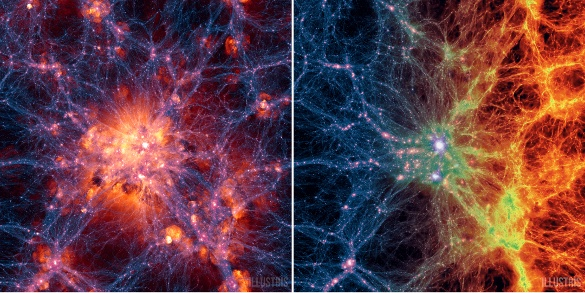
\includegraphics{img/Illustris_01.jpg}}
\thispagestyle{empty}
\newpage
\pagenumbering{arabic}
\pagestyle{plain}
\tableofcontents
\newpage

\section*{Abstract}
Whether or not the precise structure of each individual virialized DM halo in the universe today is sharply dictated by the laws of nature or a product of random mergers and collisions throughout the formation history of the universe is unknown [16].
In this sense it could be either random or determined by physics. Randomness is favored if all structures look different but physics is the fundamental driving of today's structures if we can observe common trends and universalities. This is the fundamental question being addressed. This work investigates universalities of spherical dark matter structures in equilibrium by the study of collisionless N-body systems. These systems are simulated numerically in a controlled way using the N-body code GADGET-2. The equilibrium structures are generated using Eddingtons inversion method and Osipkov-Merritt models by the means of two C-codes developed by Sparre (see [1] and [2]). Four side projects are carried out as well and can be seen in Appendix B. They address related questions, e.g. morphology of cosmological dark matter halos, how particle velocities are distributed throughout DM structures, comparison of simulated and observable quantities and finally looking for universal features in the rate of change of density profiles for different structures. 
\section*{Acknowledgements}
This work could not have been possible without the great help of my thesis supervisors Steen H Hansen and Martin Sparre. Martin has been a solid support for programming issues along the way. I believe Steen must be one of the very few supervisors who will respond to technical questions over email even late in the evening.
It has been very rewarding to work under Steen's skilled supervision as the project took several interesting directions along the way.
I am in much gratitude to the people at Dark Cosmology Center for advise and fruitful conversations.
Thanks to my family and friends for all their support. This has been a wonderful appetizer for digging further into the realms of astrophysics. \\ \\
NB: The cover image is taken from the Illustris simulation and can be found at this adress: 
\url{http://i1.ytimg.com/vi/vGpZU1LSsdY/0.jpg}
\newpage

\section{Abbreviations}
BAO:             Baryon Acoustic Oscillations \\
BBN:             Big Bang Nucleosynthesis \\
CBE: 			 Collisionless Boltzmann Equation \\
CDM: 	         Cold Dark Matter \\
CE:              Continuity Equation \\
CGS:             Centimeter-Gram-Second system \\
CMBR:            Cosmic Microwave Background Radiation \\
DE: 			     Dark Energy \\
DF: 		 	     Distribution Function \\
DM: 			     Dark Matter \\
Edd:             Eddingtons inversion method \\
EOM:             Equation Of Motion \\
FWHM:            Full Width Half Maximum (connected to Gaussian distribution) \\
HBB:             Hot Big Bang model \\
HDM: 		     Hot Dark Matter	\\
HE:  		     Hydrostatic Equilibrium  \\
HQ:              Hernquist density profile \\
JE:   		     Jeans Equation \\
LHS:             Left Hand Side \\
ln:              Natural logarithm (Logarithm with base e, Euler´s number) \\
log:             Logarithm with base 10 \\
MKS:             Meter-Kilogram-Second system (SI-units) \\
MOND:            MOdified Newtonian Dynamics \\
MW:              Milky Way galaxy \\
NFW:             Navarro-Frenck-White density profile \\
N-D:             N-dimensional/N-dimensions ($ N \epsilon \mathbb{Z}^+ $) \\
OM:              Opsikov-Merritt model \\
pct:             Percentage \\
pdf:             Probability distribution function \\
PDF:             Probability Density Function \\
PPSD:            Pseudo Phase Space Density \\
RHS:             Right Hand Side \\
ROI:             Radial Orbit Instability \\
SIMS:            Simulations \\
SM:  			 Standard Model (of particle physics) \\
SMC:  		     Cosmological Standard Model \\
STD:             STandard Deviation (of normal-distribution) \\
SUSY:            SUper SYmmetry \\
VDF: 		     Velocity Distribution Function \\
WDM: 		     Warm Dark Matter \\
wrt:             with respect to \\
$\Lambda$CDM:    Cosmological Standard Model (The so-called concordance cosmology with DE and CDM ) \\
$\mathbb{Z}^+ $: Positive integer numbers \\
\newpage
\section{Introduction}
\textbf{The purpose of this section is to elaborate a bit on the abstract and to provide a clear picture of the structure for this thesis. Starting with speculations on the nature of dark matter based on current observational constraints we can set up the appropriate theoretical framework and introduce some important concepts to describe collisionless systems. This chapter ends with the general notion of an attractor and some ideas for where to search for it in terms of dark matter systems (if it exists).} \\ \\

Advancements has been made in narrowing down the window of theoretically allowed DM particles through modern observational constraints (upper bounds to DM cross sections are lowered further as more and more DM structures aids in the vast collection of constraining structures, e.g. the bullet cluster where gravitational lensing of background objects shows two huge parts of hidden mass as remnants of the merger between two galaxy clusters with their individual dark halos (the hot X-ray gas remains in the center as it is subjected to numerous collisions intrinsically). Most astronomers believe dark matter candidates to be in the form of one or several new types of elementary particles (existing outside the current standard model of particle physics).

\centerline{\textbf{Theoretical framework}} 

\centerline{\textbf{Quantum effects are negligible}} 
Utilizing Ehrenfests theorem since the mean inter-particle distance in each simulation in the present work is larger than the particles Debroglie wavelength $\lambda = \frac{h}{p}$, we can neglect any quantum mechanical treatment and rely solely on a classical mechanical treatment for our purpose here. 
It is not known if particle collisions are important in real halos. 
Probably this will not play a role in Milky way-like galaxies but in dwarf galaxies it might [12].

\centerline{\textbf{The Newtonian limit is applicable}} 
General Relativity (GR) can also be safely neglected here, as all three conditions for taking the Newtonian limit is met ($v<<c$, $\frac{GM}{R}<<1$ in dimensionless units, and finally the structures in this work posses almost static gravitational potentials where the time-dependence is negligible). Newtonian Dynamics is therefore the appropriate theoretical framework to use (see [13] and [14]). \\

As a consequence to the fact that DM structures have a smooth density field, seem to be collisionless, and must be cold (individual particle velocities much less than the speed of light in vacuum, $v << c $. Plus we know that galaxies form befor e the formation of clusters which severely constrains the allowed ratio of hot to cold matter.), the MACHOs (MAssive Compact Halo Objects) have more or less been ruled out and WIMPS (Weakly Interacting Massive Particles) remain a top category candidate for the nature of DM. Other candidates of interest are SUper SYmmetric (SUSY) particles, axions etc. Modifications to our current understanding of gravity such as MOND or TeVeS are also considered by some. Furthermore, as any DM particle candidates obeying the above criteria (e.g. fitting in the remaining allowed energy range with a mass that is not too large) must be very numerous to account for the total density parameter value of DM (with best modern estimates, $\Omega \approx 0.23$). It is therefore necessary to have an effective measure to qualitatively describe the physical quantities of interest for the DM structures that does not depend on a detailed description of orbit etc. for each individual particle but instead treats the structures in a probabilistic manner. For this purpose the Distribution Function (DF) is introduced. The DF $f(x,v,t)$ has the three arguments of position, velocity and time. At any given time it therefore describes collective phenomena in a 6D-phasespace. The probability of finding a given particle at time t in the 6D-phasespace volume $d^3xd^3v$ is given by $f(x,v,t)d^3xd^3v$. (This gives the particle mass inside that 6D volume when multiplied by the total mass). Assuming the DM particles are belonging to just one species,i.e. they are indistinguishable, that probability is unchanged for each of the N particles inside any given DM structure. This assumption implicates a normalization for the DF at unity:
\begin{equation}
\int \! f(x,v,t) \, \mathrm{d^3}x \mathrm{d^3}v = 1
\end{equation}
Taking the Continuity Equation (CE) into account and translating it into a conservation of probability,
\begin{equation}
\frac{\partial f}{\partial t} + \frac{\partial}{\partial w}\cdot (f\dot{w}) = 0
\end{equation}
where $w = (r,v)$ and $ \dot{w} = (\dot{r},\dot{v}) = (v, a ) = (v, -\nabla \Phi ) $, where a is the acceleration and $\nabla \Phi$ is the gradient of the gravitational potential. This conservation in phase space of probability basically means, that when we follow a certain particles trajectory, the probability of finding it within a surrounding, co-moving phase space element stays the same. With the use of Hamiltons equations, the Collisionless Boltzmann Equation (CBE) can be obtained (See appendix D.4). Here written for simplicity in the form of the convective/Lagrangian derivative of the DF: \\
\begin{equation}
\frac{df(x,v,t)}{dt} = 0 
\end{equation}
Taking the 1.st moment of the CBE (Multiplying each term in the CBE by the radial momentum, and subsequently integrating over all momenta) gives us a very useful expression, namely the Jeans Equation (JE) (see derivation in appendix D.5). With no bulk motion, and assuming spherical symmetry as well as dynamical equilibrium the JE reads:
\begin{equation}
v_c^2 = -\sigma_r^2  \big[\gamma +\kappa +2 \beta \big] 
\end{equation}
with the circular velocity,
\begin{equation}
v_c^2 = \frac{GM}{r}
\end{equation}
There is evidence pointing to the fact that dark matter might be collisionless described by the velocity anisotropy parameter, 
\begin{equation}
\beta \equiv 1 - \frac{\sigma_{tan}^2}{2 \sigma_{rad}^2} 
\end{equation}
where $\sigma_{tan}$ and $\sigma_{rad}$ are the tangential and radial velocity dispersions, respectively. It is known from cosmological simulations that $\beta$ increase from zero at the center of a halo to about $\beta \approx 0.25$ at $r_{-2}$, which is the radius where $\gamma = -2$, with the radial slope of the density profile , 
\begin{equation}
\gamma \equiv \frac{d\ln\rho}{d\ln r}
\end{equation}
finally the radial slope of the radial velocity dispersion is defined as
\begin{equation}
\kappa = \frac{d\ln\sigma_r^2}{d\ln r} 
\end{equation}
The JE thus closely resembles the formula for Hydrostatic Equilibrium (HE), which becomes more clear if $\sigma_r^2$ is interpreted as temperature and $\kappa$ thus becomes the radial part of the temperature gradient. 

\begin{figure}[!htbp]
\centering
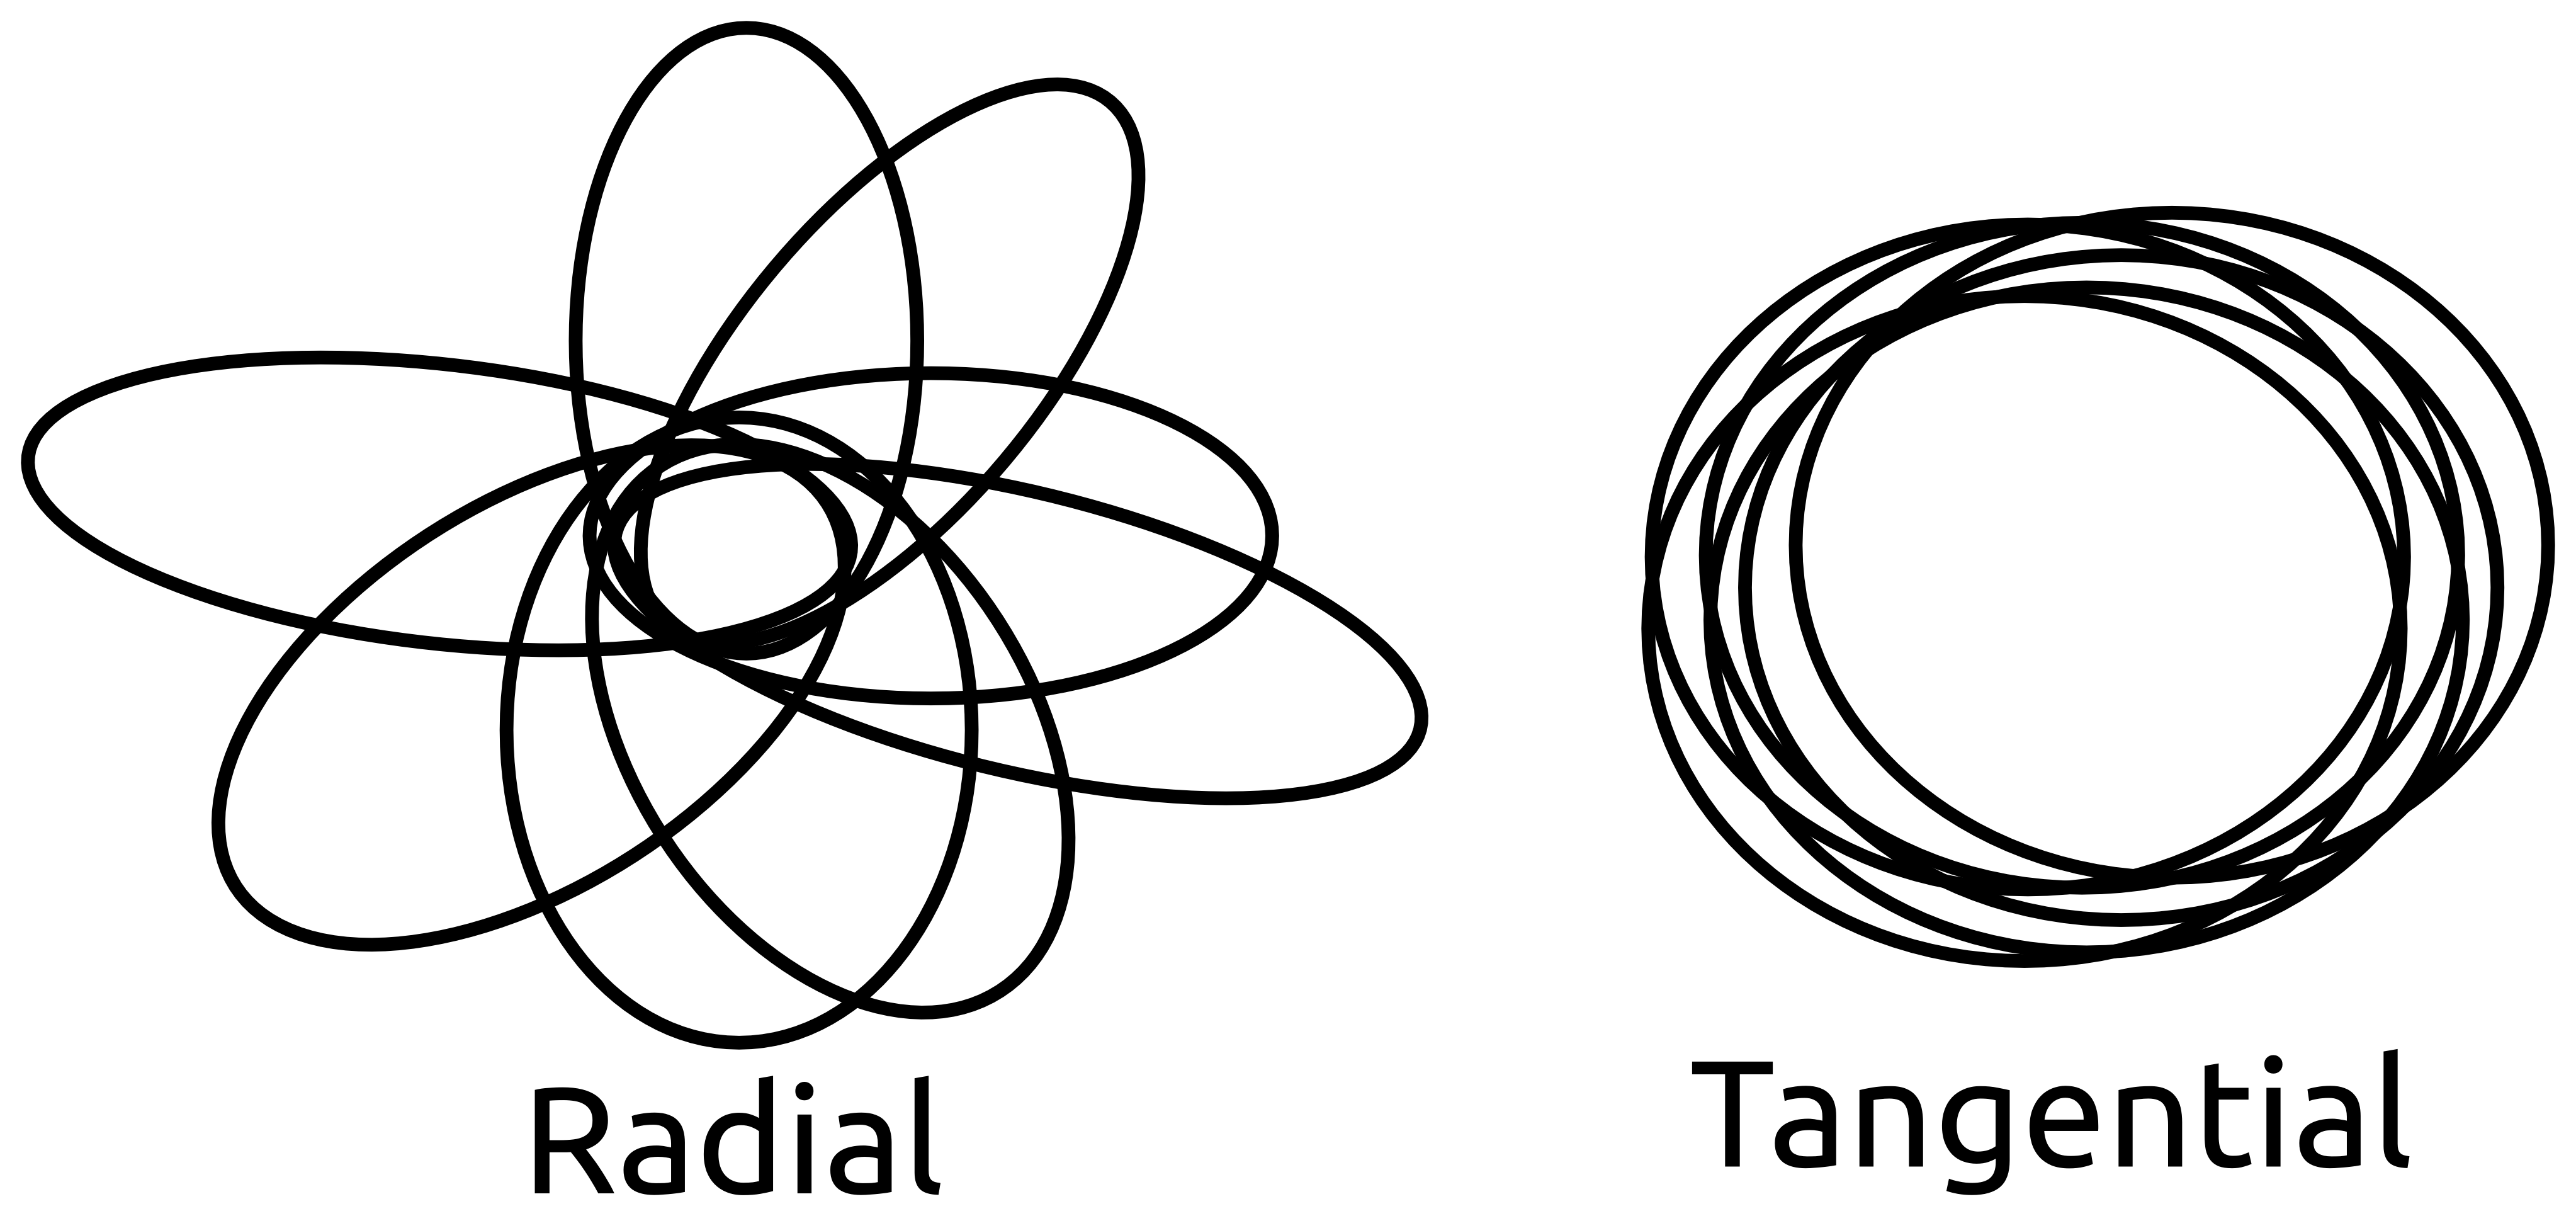
\includegraphics[width=1.0\linewidth]{Thesis_Final_Version/img/orbit.png}
\caption{Radially biased vs. tangentially biased bound orbits for spherical potential. The purely radial orbits correspond to a $\beta$-value of unity, whereas the purely tangential orbits correspond to a $\beta$-value of $- \infty$ (isotropic structures would have $\beta$ equal to zero). The morphology of cosmological DM halos tend to be either oblate or prolate thus giving rise to direction dependent velocity anisotropy, but as structures created for this work is very close to spherical such directional dependence can be safely neglected and thus $\beta$ can reasonably accurately be computed as a spherical average inside radial bins which is the main analysis strategy of choice (mass bins and velocity bins are also tested).}
\label{fig:test}
\end{figure}

The JE gives us the total mass enclosed within a certain radius. As there is only one equation but three free parameters it is in general very hard to solve and a step closer to this goal will be finding universalities between those three parameters. \\ \\
\textbf{Characteristic timescales} \\
The following characteristic timescales are usually of interest in astrophysical contexts: \\
The time it takes for a particle with velocity v to cross a structure of radius R once, known as the crossing time: 
\begin{equation}
t_{cross} = \frac{R}{v}
\end{equation}
The relaxation time, given by $ t_{relax} = n_{relax}t_{cross} $ where $ n_{relax} \approx \frac{N}{8\ln\Lambda} $ is the number of crossings necessary to change the velocity by of order itself.
The $\Lambda$ comes from the Coulomb logarithm defined by $ ln\Lambda \equiv \ln(\frac{b_{max}}{b_{min}})$ (where b is the impact parameter) and can be simplified into 
\begin{equation}
\Lambda = \frac{R}{b_{90}} \approx \frac{Rv^2}{Gm} \approx N 
\end{equation}
So we can write: 
\begin{equation}
t_{relax} \approx \frac{0.1N}{\ln N}t_{cross} 
\end{equation}
The dynamical time is defined as: 
\begin{equation}
t_{dyn} = \sqrt{G \bar{\rho}}  
\end{equation}

\centerline{\textbf{Attractors}} 
Attractors are observed several places in nature. Chaos theory deals with dynamical systems and their properties such as attractors and repellers. The general idea of an attractor arise in the study of dynamical systems. It can be described as a set or group of numerical values (in the form of either points, curves, manifolds, or a strange attractor which have fractal structure) that a system will evolve towards. This should be true for a large span of IC's of the system. 
chaos theory creates a mathematical framework of dealing with chaotic dynamics and corresponding attractors. An attractor is connected with a so-called basin, which is a region surrounding it for which system values that gets near the attractor will remain close even if slightly perturbed. The condition for any attractor is that the trajectory of any dynamical system it contains never leaves the attractor as time goes. This opens up two possibilities for these bound trajectories; periodicity or chaos. If a basin contains dynamical systems flowing away from any given set, that set is on the contrary called a repeller. In summary, an attracting set for any dynamical system is a closed subset of its phase space such that for many different IC's the system will evolve towards that closed subset. Even if an attractor for cosmological collisionless structures does exist in nature, it might be that it will only be seen in the central part of the structure if only this part of the structure has reached equilibrium. Here is a big advantage in computing numerical simulations since we can create a structure in dynamical equilibrium for which, if an attractor does exist, the attractor might be visible throughout the whole structure. Different attractors are found in nature. A star is a good example; On a Hertzsprung Russell diagram which show luminosity vs. surface temperature for stars, it is clear that an attractor exist. It is referred to as the stars main sequence. So the question is where to search for an attractor for DM systems. Since we have the Jeans Equation giving us the total mass, described by the three Jeans parameters $ \gamma$, $\kappa$ and $\beta$, which is just one equation for which there exist an infinite set of different solutions (possible combinations of the three parameters, for any fixed mass), this motivates searching for an attractor in $ (\gamma, \kappa, \beta) $-space. \\
Other known DM universalities exist as well, e.g. the pseudo phase space density is a powerlaw in radius $\frac{\rho}{\sigma^3}=r^{-\alpha}$ (Taylor and Navarro, 2001) and the linear relation $\gamma = 0.2(\beta - 0.8)$ (Hansen and Moore, 2006).

\textbf{With these proper tools in hand (J.E. etc.) and knowing what to search for (attractors in the Jeans parameter space), the strategy is to set up different Initial conditions spanning as large a volume in the parameter space as possible, choosing important physical processes in our universe to mimic with computer simulations (after plugging in these Initial conditions), comparing the outcome of each structure when subjected to these simulations and thus searching for universal trends or attractors. The next section will cover some important physical processes which can be used as a blueprint for creating different computer simulations.}
\newpage
\section{Mergers in the universe}
\textbf{Mergers are important phenomena since they occur frequently throughout cosmic history and contribute to the shaping of structures observed today. When a galaxy first forms or when galaxies merge together they are out of equilibrium. During the structure formation and evolution of the universe, mergers of galaxies and other objects happens frequently. Such mergers cause phase mixing and violent relaxation which are both collisionless relaxation processes. They drive each other when a system undergoes collapse; e.g. during galaxy formation} \\ \\

\subsection{Phase mixing}
The CBE is satisfied during galaxy mergers. Phase mixing is the process where regions of lower phase space density is mixed together with regions of higher phase space density. It is important when a galaxy relaxes towards a steady state, and it works by changing the coarse-grained phase-space density near the phase point of each star. Phase mixing and the CBE has the combined effect of making the maximum value of the DF decrease in a monotonic way. The systems mass fraction positioned at DF values above any value is reduced. [3]

\subsection{Violent relaxation}
Violent relaxation changes the energy of each star in a given galaxy. 
When the gravitational potential $\Phi (x,t)$ of a given galaxy depends both on position and time, The corresponding energy is changing with time in the following way: \\
\begin{equation}
\frac{d E}{d t} = \frac{\partial \Phi}{\partial t} \bigg|_{x(t)}
\end{equation}
This is what Simulation type II tries to do by providing a kick-flow pattern of energy exchange and subsequent drift.
Violent relaxation widens the range of energies for the particles. Whether the energy of a given particle will increase or decrease depends on starting position and velocity but is independent of the particles own mass. This makes collision-less systems significantly different from gas systems where equipartition of energy happens as time goes and a gas system reaches thermal equilibrium. Mergers of galaxies or halos is simulated by type I. More on this in a later section.

\textbf{With the understanding of these effects we are prepared to set up simulations that mimic these effects. First we will see some density models in the following section which accurately describes dark halos and subsequently use some of these density models together with other parameter choices to create a large set of both stable and unstable Initial Conditions in the following section.}
\newpage
\section{Double-power density models}
\textbf{Power laws provide excellent descriptions of several astronomical objects;
e.g. a double power law in radius can account for the luminosity density of elliptical galaxies at all radii. Transitioning between large and small radii is described by a model constant, $\gamma$, which is typically set to unity. Dark matter structures has been shown by numerical simulations to be well accounted for wrt. their mass density, by double power laws as well [1].} \\ \\

\centerline{\textbf{Cusp/Core Controversy}} 
The cusp/core problem is relevant when choosing a density profile. In simulations we see a higher degree of halos with central cusps (where $\gamma = -1$), but observations indicate that dwarf galaxies tend to have central cores instead (with $\gamma = 0$). The NFW-profile has a cusp, whereas the Einasto profile has a more flattened central form. The reason for using a HQ density profile instead of a NFW lies in the fact that the HQ has a finite mass, whereas the NFW needs a cut-off. Any physical model for the density must satisfy these conditions: The density profile should be non-negative and finite everywhere in space. It has to decrease smoothly and tend to zero at very large radii. Taking some moments of the mass function, they must be finite, e.g. moments that define the central potential, the total mass, and the effective radius of the system. Finally, the analytical/descriptive functions has to be continuous (no jump discontinuities). Einasto found several groups of descriptive functions where the above criteria are being fulfilled, but the Einasto-profile agrees best with observations. \\

The double power laws described here have the form
\begin{equation}
\rho(r) = \frac{\rho_0}{(\frac{r}{r_s})^{\alpha}(1+(\frac{r}{r_s})^{\gamma})^\frac{\beta-\alpha}{\gamma}}  
\end{equation}
with the transition, $\gamma=1$ for this work.
Most initial structures (see tables of simulations) are set up to follow Hernquist (hereafter HQ) density profiles [22], i.e. \\
\begin{equation} 
\rho_{HQ}(r) = \frac{\rho_0}{(\frac{r}{r_s})(1+\frac{r}{r_s})^3}  
\end{equation}
This is the mass distribution which has been suggested for spherical galaxies by Hernquist in 1990. The normalization constant is given by $\rho_0 = \frac{M}{2\pi}$ , where M is the total mass. For all HQ structures in this work, $M = 1$. Therefore $\rho_0 = \frac{1}{2\pi}$ and the Hernquist profile is simply:
\begin{equation} 
\rho(r) = \frac{1}{2\pi r(1+r)^3}  
\end{equation}
The characteristic scale radius $r_s $ is set to unity throughout. It gives a good description of halo structures. The HQ profile closely resembles the NFW density profile [23], \\
\begin{equation}
\rho_{NFW}(r) = \frac{\rho_0}{(\frac{r}{r_s})(1+\frac{r}{r_s})^2}  
\end{equation}
which has been shown to fit halos in cosmological simulations under a wide range of circumstances. The two mass models differ only for large r, \\
where the NFW profile is diverging towards infinite mass but the HQ profile converges towards a finite mass (Hernquist 1990). 
It turns out that the inner part of structures is insensitive to this difference. It is therefore safe to use either of these two halo profiles if one of them is known to provide a good description of the structure in question. Another density distribution used here is a double power model with $\alpha = 0$ and $\beta = 5$ which takes the form
\begin{equation} 
\rho_{0,5}(r) = \frac{\rho_0}{(1+r)^5}  
\end{equation}
Since the main goal is to determine if an attractor exist in the Jeans parameter space, different density models are needed and starting from a range of different IC's is crucial to determine if they all flow towards any preferred universality for two different types of simulations (here called I and II). In order for this distribution to get a mass of unity, the normalization constant must be $\rho_0 = \frac{3}{\pi}$. The mass of the HQ and NFW profiles are:
\begin{equation}
%\[
    M(r)= 4\pi \rho_0 a^3  
\begin{cases}
    \frac{(\frac{r}{a})^2}{2(1+\frac{r}{a})^2},& \text{HQ} \\
    \ln(1 + \frac{r}{a}) - \frac{\frac{r}{a}}{1 + \frac{r}{a}},& \text{NFW}
\end{cases}
%\]
\end{equation}
Which with normalized total mass and $r_s$ becomes
\begin{equation}
%\[
    M(r)= 2  
\begin{cases}
    \frac{r^2}{2(1+r)^2},& \text{HQ} \\
    \ln(1+r) - \frac{r}{1 + r},& \text{NFW}
\end{cases}
%\]
\end{equation}
And the mass for the $(\alpha,\beta)=(0,5)$ profile is:
\begin{equation} 
M(r) = \int_{0}^{R} \! \rho \cdot 4\pi r^2 \, \mathrm{d}r = 
 \frac{r^3(r+4)}{(r+1)^4}
\end{equation}
With the limit
\begin{equation} 
\lim_{r \to +\infty} M = 1
\end{equation}
Which is thus the total mass of structures D1, DS1 and D2. As their particle number are $N = 10^5$, each particle in these 3 Sims have a mass of $m = \frac{1}{6} \cdot 10^{-5}$. A check is provided that plots the numerically computed density together with the analytical expression for the density profile. The two are in good agreement and this is a good support of the C-codes used.
\begin{figure}[!htbp]
\centering
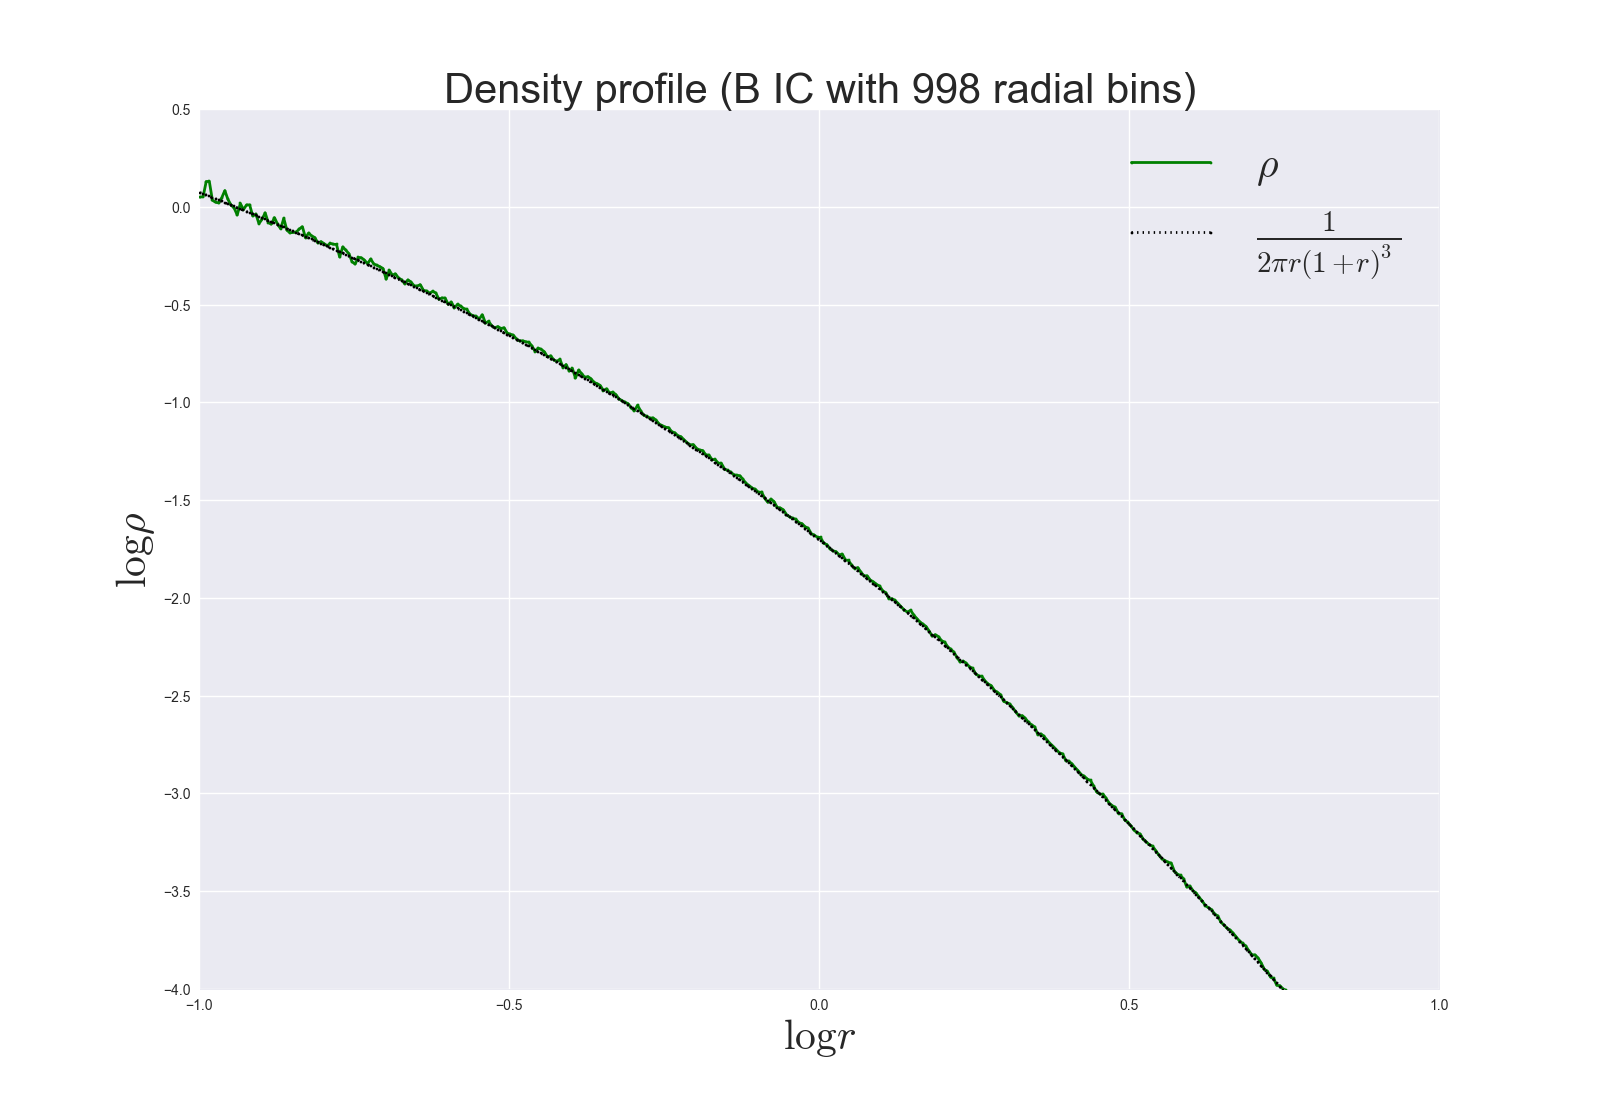
\includegraphics[width=1.0\linewidth]{img/B_Density_fit.png}
\caption{$\rho$ for IC of structure B shown together with analytical expression of HQ profile. The two are in good agreement. Notice the fluctuations at small radii; these can be attributed to Poisson noise. 998 radial bins is used. This structure has a total mass of unity and $N=10^6$ particles, and each particle has a mass of $10^{-6}$ in some arbitrary mass-unit.}
\label{fig:test}
\end{figure}
Since the $\gamma$ profile for all stable structures in dynamical equilibrium have one unique radius where it equals the value -2, hereafter denoted as $r_{-2}$, this radius is a good quantity to normalize radii by in order to better compare different structures. It further introduces a natural unit of length.
\newpage
\section{Generating initial structures}
\textbf{Two different methods are used to distribute particles and provide them with initial velocities. One generates completely isotropic structures, the other tunes the degree of velocity anisotropy by a free parameter.} \\ 

\subsection{Eddingtons inversion method}
\textbf{Eddingtons inversion method is used to construct isotropic spherical models.} \\ 

If we know the density profile of a spherical structure with potential $\Phi(r)$ then a unique DF depending on the phase-space coordinates only through the Hamiltonian H(x,v) can be found. As it depends only on the energy this DF f($\mathcal{E}$) is ergodic and has $\beta = 0$ everywhere by definition. Introducing the relative energy 
\begin{equation} 
\mathcal{E} \equiv -\Phi+\Phi_0
\end{equation}
and relative potential 
\begin{equation} 
\Psi \equiv -H+\Phi_0 = \Psi - \frac{1}{2}v^2
\end{equation}
The PDF $\nu(r)$ is the integral of f over all velocities.  
\begin{equation} 
f(\mathcal{E}) = 4\pi \int \! v^2 f(\Psi - \frac{1}{2}v^2) \, \mathrm{d}v =
4\pi \int_{0}^{\Psi} \! f(\mathcal{E}) \sqrt{2(\Psi - \mathcal{E})} \, \mathrm{d}\mathcal{E} =
4\pi \cdot \sqrt{2} \int_{0}^{\Psi} \! f(\mathcal{E}) \sqrt{\Psi - \mathcal{E}} \, \mathrm{d}\mathcal{E}
\end{equation}
Transforming $\nu(r) \rightarrow \nu(\Psi)$ and rearranging (also using $4 \sqrt{2} = 2 \sqrt{8}$),
\begin{equation} 
\frac{1}{\sqrt{8}\pi}\nu(\Psi) = 2\int_{0}^{\Psi} \! f(\mathcal{E}) \sqrt{\Psi - \mathcal{E}} \, \mathrm{d}\mathcal{E}
\end{equation}
Differentiating the above equation wrt $\Psi$ and solving the following Abel integral equation we obtain Eddington's formula which gives us the corresponding distribution function,
\begin{equation} 
f(\mathcal{E}) = \frac{1}{\sqrt{8}\pi^2}\frac{\mathrm{d}}{\mathrm{d}\mathcal{E}}
\int_{0}^{\mathcal{E}} \! \frac{d \Psi}{\sqrt{\mathcal{E}-\Psi}} \, \frac{\mathrm{d}\nu}{\mathrm{d}\Psi} 
\end{equation}
To see this derivation in more details, see [3].
A C-code made publicly available by Martin Sparre is used for this purpose [1]. It takes a density model as argument and uses it to distribute particles and provide them with initial velocities.
\begin{figure}[!htbp]
\centering
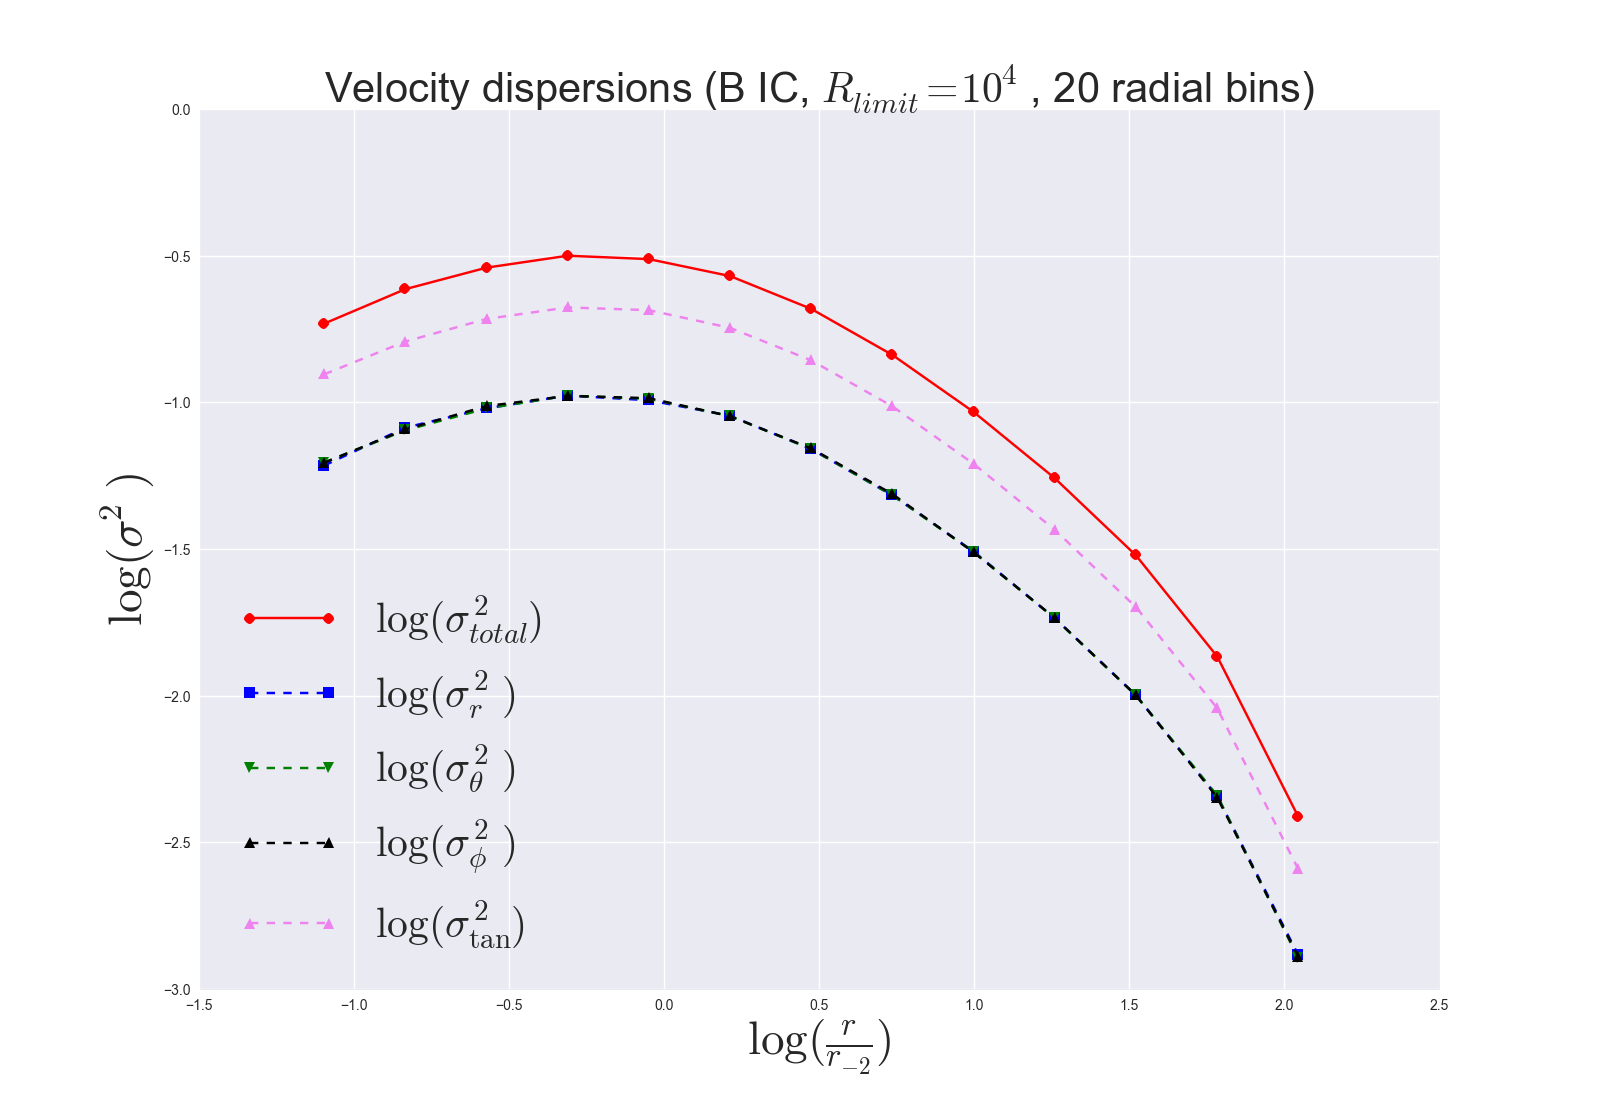
\includegraphics[width=1.0\linewidth]{img/B_IC_sigma_r_2.png}
\caption{$\log (\sigma^2)$ vs. $\log (\frac{r}{r_{-2}})$ for IC of structure B. 20 radial bins is used and the structure is cut off at radius $R_{limit} = 10^4$ in arbitrary units of radius. Notice how each of the dispersions $\sigma_r^2$, $\sigma_{\theta}^2$ and $\sigma_{\phi}^2$ contributes equally to the total velocity dispersion. This is due to the fact that the IC of structure B is completely isotropic (as is the case for any Eddington profile) and therefore $\sigma_r^2 = \sigma_{\theta}^2 = \sigma_{\phi}^2$. This is true throughout all radii of the structure. The pink curve shows the tangential part, $\sigma_{tan}^2 = \sigma_{\theta}^2 + \sigma_{\phi}^2$.}
\label{fig:test}
\end{figure}

\begin{figure}[!htbp]
\centering
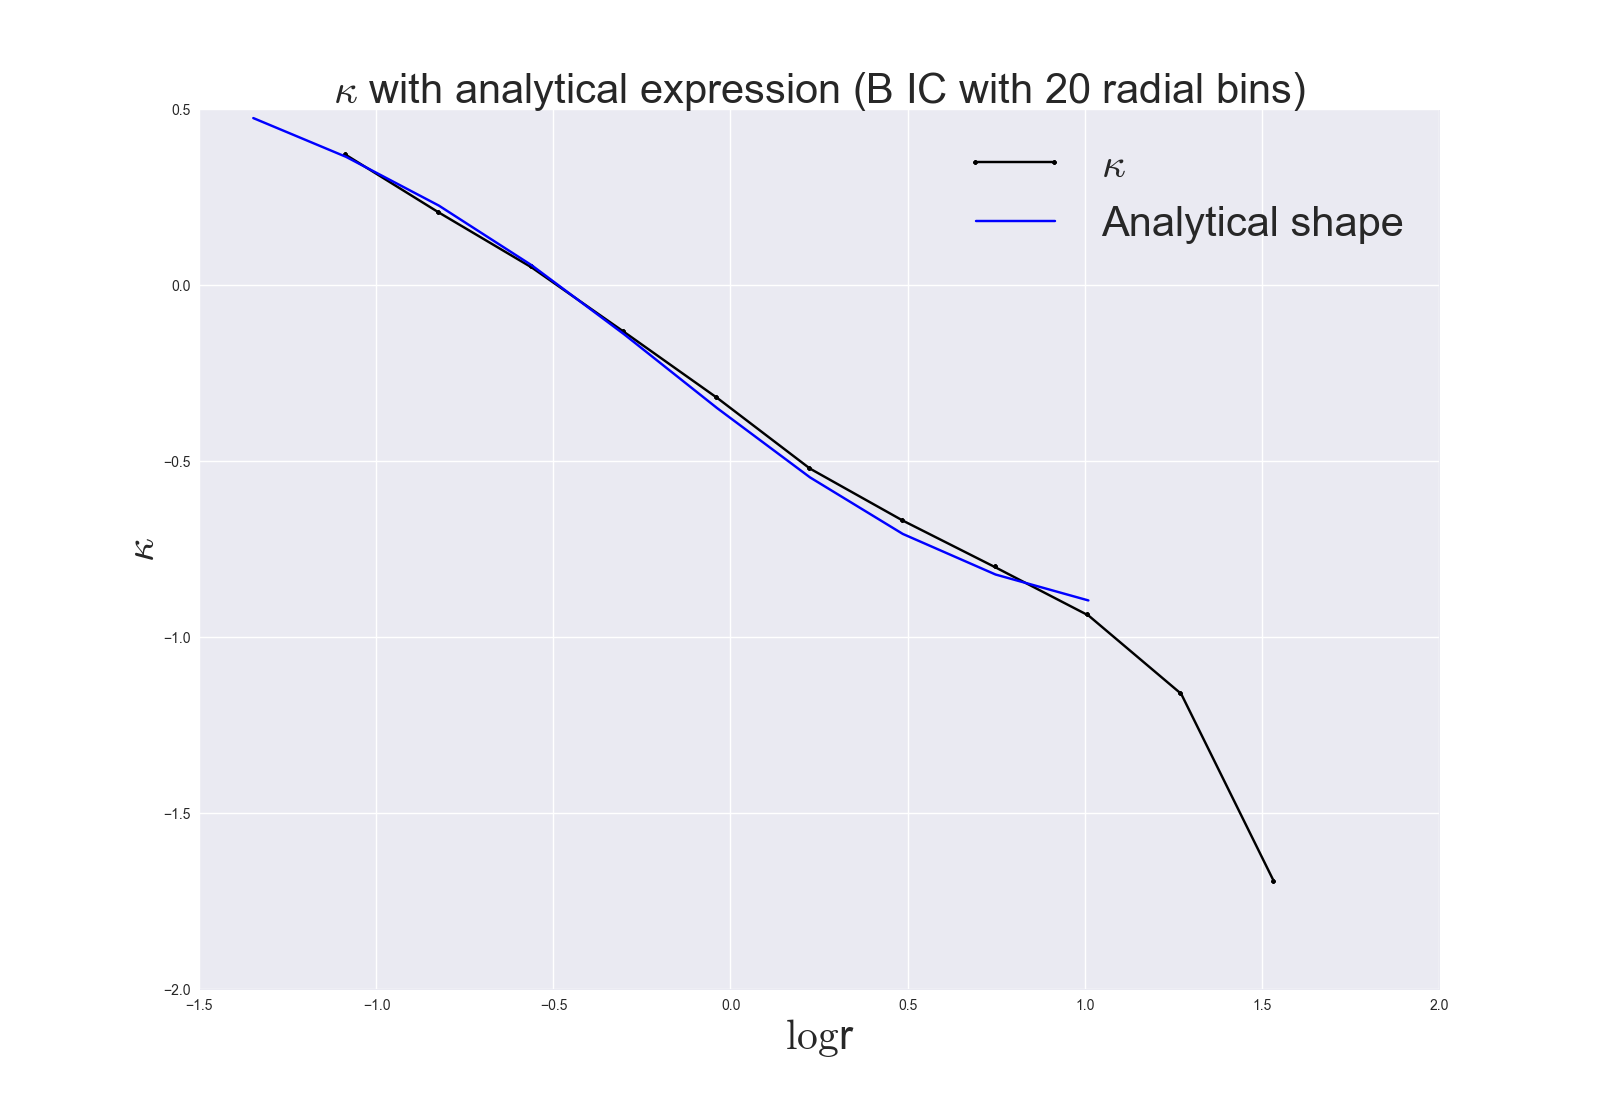
\includegraphics[width=1.0\linewidth]{img/B_IC_kappa_logr_fit.png}
\caption{$\kappa$ for IC of stable structure B shown together with the analytical expression. 20 radial bins is used. This provides a welcome consistency check of the C-codes used from [1] and [2]. The analytical expression is seen to be in good agreement with the structure generated by means of these codes. The analytical expression is truncated around $\log r = 1$ as the two curves starts to depart from each other here. This could be due to different reasons, e.g. the initial value chosen numerically when solving the differential equation arising from the Jeans equation when isolating $\sigma_r^2$ might be needed at higher accuracy or perhaps outer parts of the IC generated using Eddingtons method departs slightly from equilibrium due to the large distances between particles here. The majority of the IC is seen to be in good agreement though.}
\label{fig:test}
\end{figure}

\begin{figure}[!htbp]
\centering
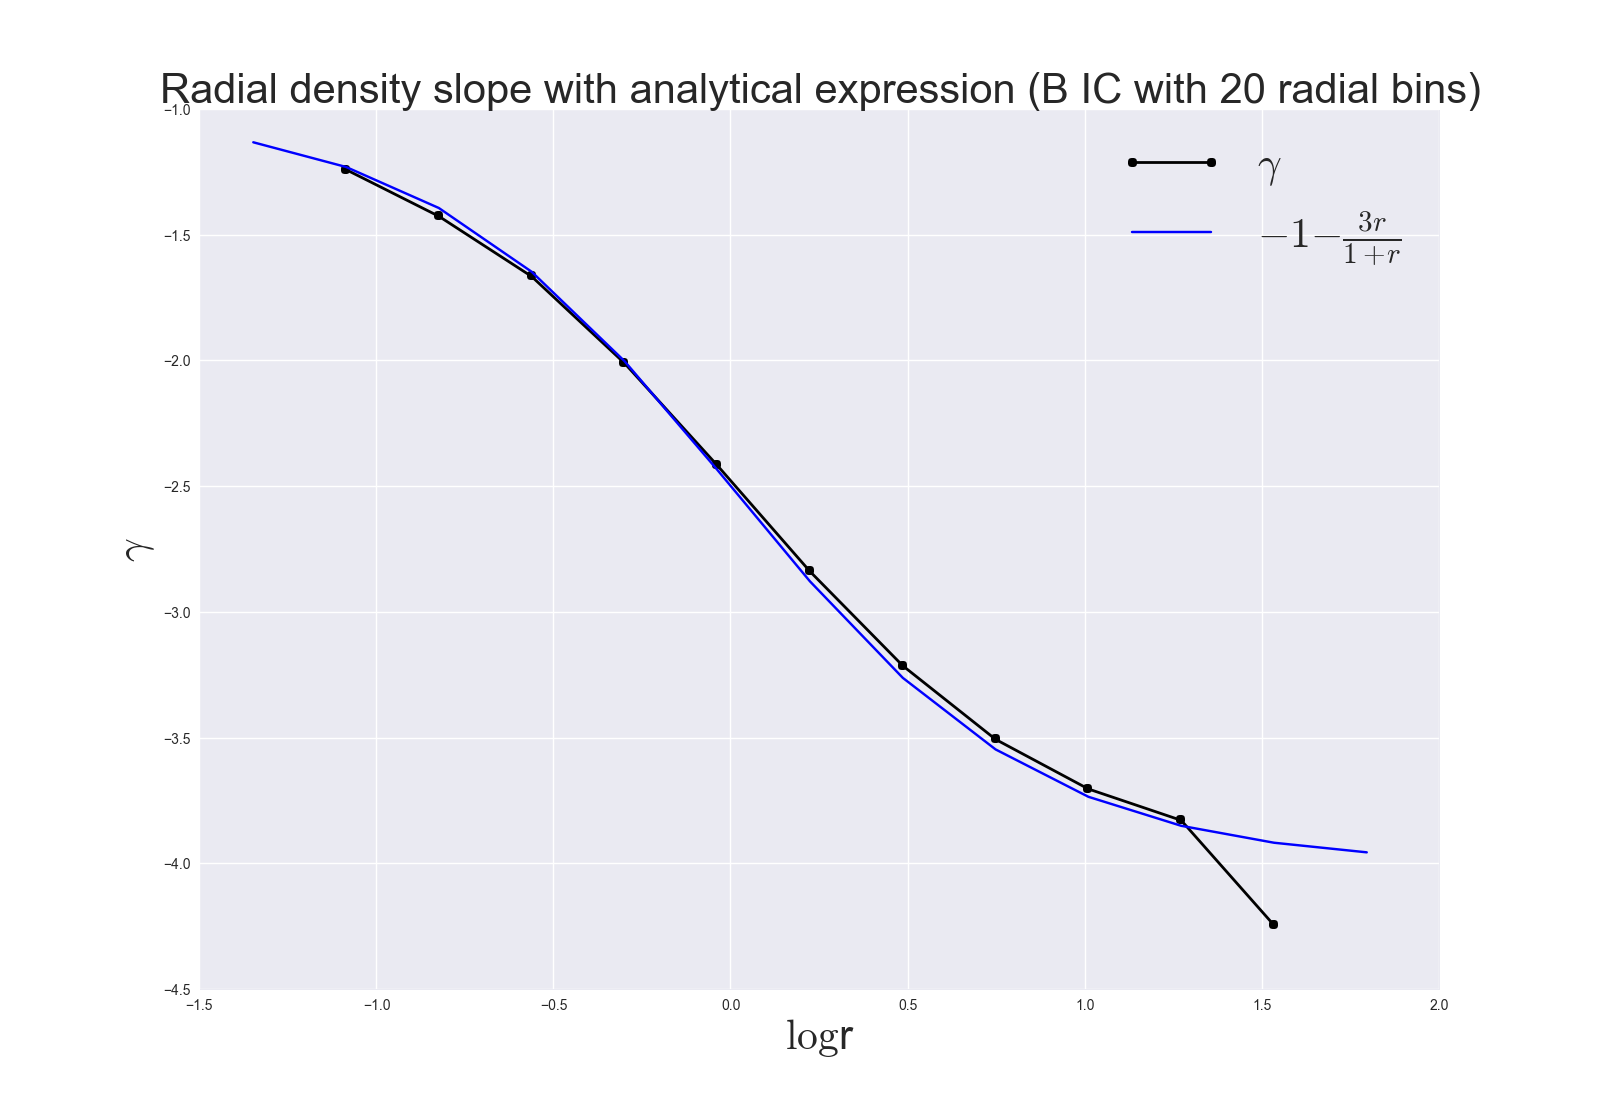
\includegraphics[width=1.0\linewidth]{img/B_IC_gamma_logr_fit.png}
\caption{$\gamma$ for IC of structure B shown together with the analytical expression $\gamma = -1-\frac{3r}{1+r}$. 20 radial bins is used. This provides a welcome consistency check of the C-codes used from [1] and [2]. The analytical expression is seen to be in good agreement with the structure generated by means of these codes.}
\label{fig:test}
\end{figure}

Checks for the validity of the Eddington profiles and the Osipkov-Merritt models (see next section) generated from the C-codes [1] and [2] is provided here graphically by means of over-plotting the Jeans parameter profiles and their corresponding analytical expressions. The results from the C-codes and the analysis codes developed for this work are thus seen to be in good agreement (see figure 4-6).

\centerline{\textbf{Analytical expression of $\gamma$:}}
For a Hernquist density model with scale radius $r_s = 1$,
\begin{equation} 
\rho_{HQ}(r) = \frac{\rho_0}{r(1+r)^3}  
\end{equation}
The natural logarithm can be applied to both sides,
\begin{equation} 
ln(\rho) = ln \Bigg[ \frac{\rho_0}{r(1+r)^3} \Bigg] = ln(\rho_0) - ln(r(1+r)^3)
\end{equation}
Setting $\rho_0 = 1$,
\begin{equation} 
ln(\rho) = - ln(r(1+r)^3) = - ln(r) -3ln(1+r)
\end{equation}
$\gamma$ is defined as 
\begin{equation}
\gamma \equiv \frac{d\ln\rho}{d\ln r} = r\cdot \frac{d\ln\rho}{dr} = 
r\cdot \Bigg( -\frac{1}{r}-3\cdot \frac{1}{1+r} \Bigg) =
-1-\frac{3r}{1+r}
\end{equation}
which is thus the analytical expression.
This can be seen in figure 5 to agree very well with the IC of Eddington structure B.


\centerline{\textbf{Analytical expression of $\kappa$:}}
This Jeans parameter can be derived analytically by solving the differential equation arising when $\kappa = -\frac{d\ln\sigma_r^2}{d\ln r} $ is isolated from the Jeans Equation assuming e.g. a Hernquist density profile. As we are considering isotropic models here, $\beta = 0$ and J.E. reads

\begin{equation}
M(r)= -\frac{r \sigma_r^2}{G} \big[\gamma +\kappa] 
\end{equation}
rearranging,
\begin{equation}
-\frac{GM}{r} = \sigma_r^2 \big[\gamma +\kappa] 
\end{equation}
isolating $\kappa$,
\begin{equation}
\kappa = -\frac{GM}{r \sigma_r^2} - \gamma
\end{equation}
using the definition,
\begin{equation}
\kappa = \frac{d\ln\sigma_r^2}{d\ln r} = \frac{r}{\sigma_r^2}\cdot \frac{d \sigma_r^2}{dr}
\end{equation}
equating the two expressions for $\kappa$,
\begin{equation}
\frac{r}{\sigma_r^2}\cdot \frac{d \sigma_r^2}{dr} = -\frac{GM}{r \sigma_r^2} - \gamma
\end{equation}
multiplying both sides by $\frac{\sigma_r^2}{r}$,
\begin{equation}
\frac{d \sigma_r^2}{dr} = -\frac{GM}{r^2} - \frac{\gamma \sigma_r^2}{r} 
\end{equation}
which can then be solved for $\sigma_r^2$ when inserting the analytical expression for $\gamma$ found above and when using the initial value of \[ \lim_{r \to \infty} \sigma_r^2 = 0 \] (which can be approximated numerically as e.g. (r,$\sigma_r^2$) = ($10^5$,$10^{-5}$) to solve computationally).
After $\sigma_r^2$ is found, $\kappa$ is determined by the definition $\kappa = -\frac{d\ln\sigma_r^2}{d\ln r} $, in a similar fashion as the one utilized for deriving $\gamma$ above.
The resulting expression is very long so it is omitted here but can be seen in figure 4 to agree very well with the IC of Eddington structure B (to see the full analytical expression go to the link for my analysis codes given in the conclusion to this project).

\subsection{Osipkov-Merritt models}
\textbf{This method generalizes Eddington's formula. Whereas Eddington's formula simply creates isotropic structures, OM models can have anisotropy as well.} \\ 

Spherical stellar systems such as galaxies and star clusters as well as dark matter halos can be represented mathematically by OM models. Ansatz: The DF depends on another function, Q: $f(Q) = f(\mathcal{E} - \frac{L^2}{2r_a^2})$ This creates DF's in phase-space which belong to specified density profiles; e.g. of a DM halo, in a predefined gravitational potential. The degree of velocity anisotropy is adjusted by the anisotropy radius $r_a$. When the minimum value $r_a=0$ is used, the model will be isotropic and produce the same outcome as Eddington's method. At the other extreme, when $r_a=\infty$, the model will consist of purely radial motions. The OM DF has the form
\begin{equation} 
f(Q) = \frac{1}{\sqrt{8}\pi^2} \Bigg[ \int_{0}^{Q} \! \frac{\mathrm{d} \Psi}{\mathrm{d} \sqrt{Q-\Psi}}
\frac{\mathrm{d}^2 \nu_Q}{\mathrm{d} \Psi^2} + \frac{1}{\sqrt{Q}} \Bigg( \frac{\mathrm{d} \nu_Q}{\mathrm{d} \Psi} \Bigg)_{\Psi=0} \Bigg]
\end{equation}
The anisotropy parameter is given by 
\begin{equation} 
\beta(r) = \frac{1}{1+(\frac{r}{r_a})^2}
\end{equation}
This gives a structure which has $\beta = 0 $ for $r<<r_a$ and radially biased for $r>>r_a$ I am using a C code made publicly available by Martin Sparre [2].
\begin{figure}[!htbp]
\centering
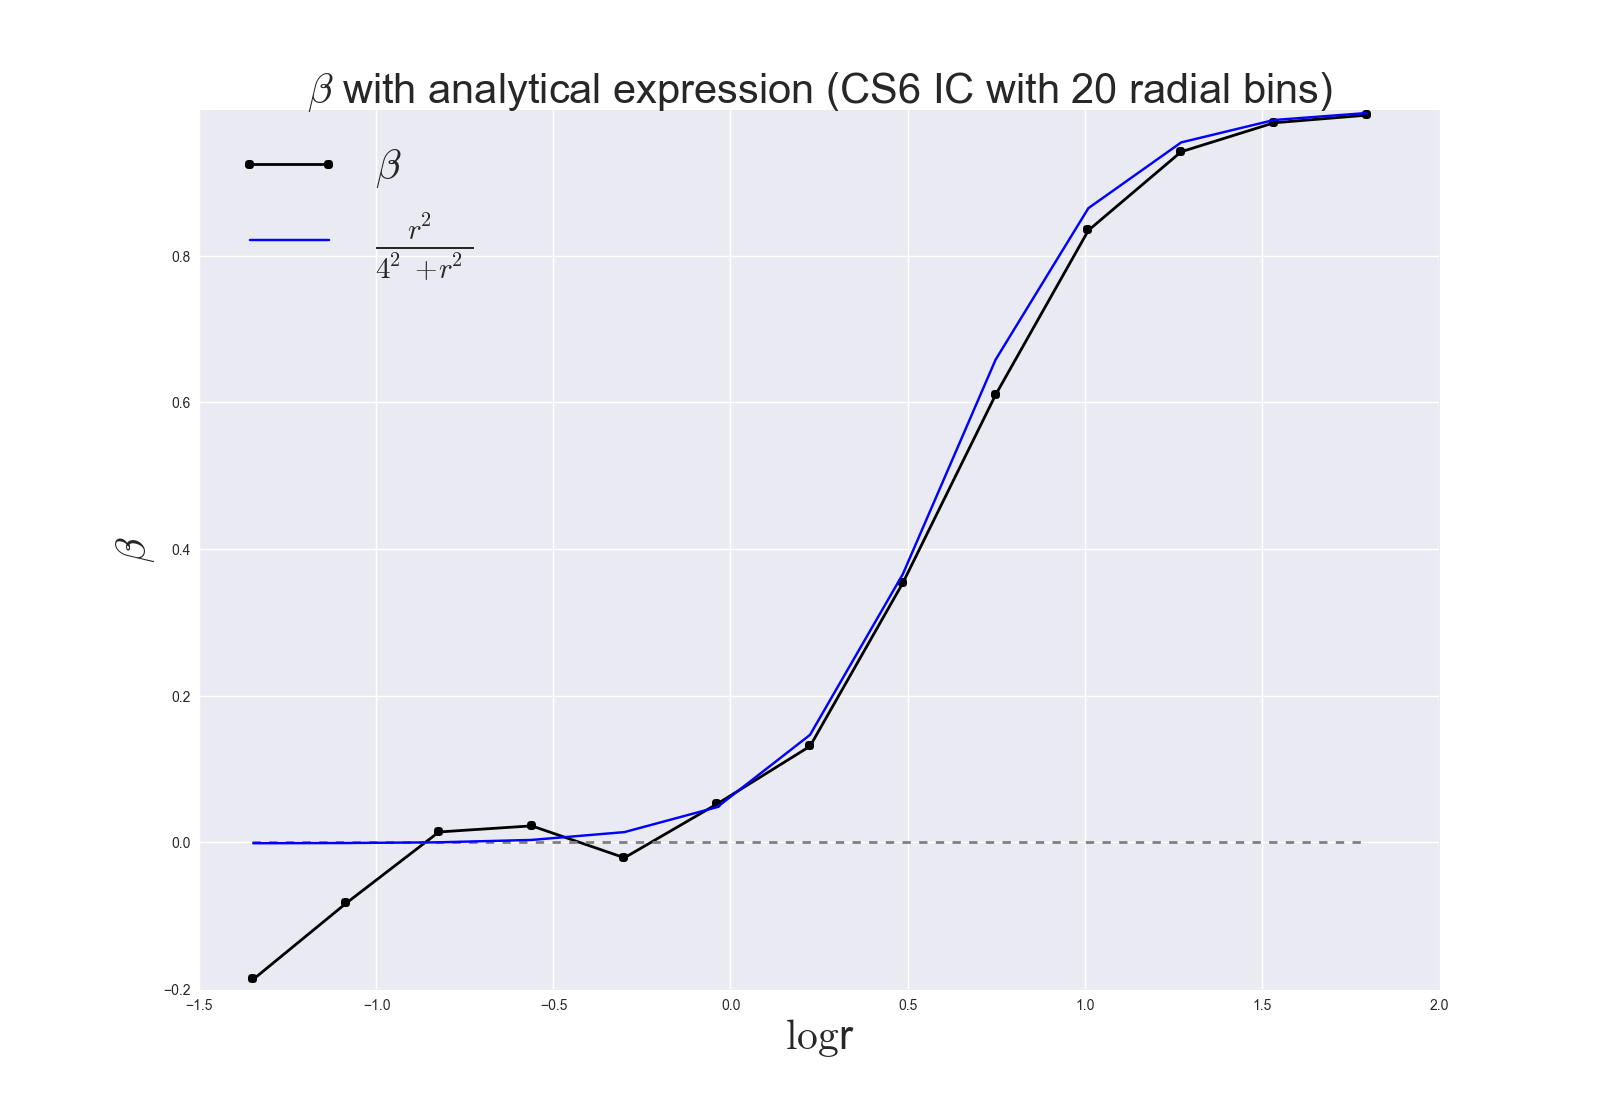
\includegraphics[width=1.0\linewidth]{img/CS6_IC_beta_logr_fit.png}
\caption{$\beta$ for IC of structure CS$\_$6 shown together with the analytical expression $\beta(r)=\frac{r^2}{r_a^2+r^2}$. It is seen that the analytical expression agrees well with the computed velocity anisotropy for the anisotropy radius $r_a = 4.0$, which is the value specified for the IC of the CS$\_$6 structure. 20 radial bins is used.}
\label{fig:test}
\end{figure}

\centerline{\textbf{Analytical expression of $\beta$:}}
The $\beta$ expression for an OM model is simply given by $\beta(r)=\frac{r^2}{r_a^2+r^2}$ so if we choose to set $r_a = 1$, the analytical form becomes just $\beta(r)=\frac{r^2}{1+r^2}$ which can be seen in figure 6 to agree very well with the IC of OM model CS$\_$6.

\subsection{Overview of structures}
\textbf{All structures can be divided into two categories, namely stable or unstable (see tables). Most of them follow Hernquist density profiles (see previous section) but three follow the $(\alpha, \beta) = (0,5)$ density profile. The unstable structures are dealt with in the later section 'Unstable OM models'. ICs have been chosen so that they together span a large volume in the 3D Jeans parameter solution space ($\beta, \gamma, \kappa$). This creates an opportunity to test if they all keep spanning a large volume or flow towards an attractor.} \\ 

Since all HQ structures have a total mass of unity but vary in particle number, the more numerous structures have particles with lower mass. Variations in anisotropy radius are carried out while setting up the different OM models. Gravitational softening is varied so that it decreases by a factor when particle number is increased (see tables). For all simulations, the scale radius $r_s = 1$ is used and $\rho_0 = \frac{1}{2 \pi}$ (which ensures that all HQ structure has a total numerical mass value of 1). The type of simulation each structure is undergoing is indicated by I: 'Instantaneous change in the gravitational potential' and II: 'Energy exchange' (See later sections for description of I and II). 
\begin{table}[!htbp]
\centering
\begin{tabular}{|c|c|c|c|c|c|c|c|c|c|c|c|}
\hline
 &A&B&$CS_1$&$CS_2$&$CS_3$&$CS_4$&$CS_5$&$CS_6$&$DS_1$&$D_2$&E \\ \hline
 N &$10^6$&$10^6$&$10^4$&$10^4$&$10^4$&$10^5$&$10^5$&$10^5$&$10^5$&$10^5$&$10^6$ \\ \hline
 IC&Edd&Edd&OM& OM & OM & OM & OM & OM & OM & Edd & OM                \\ \hline
 $\rho$ & HQ & HQ & HQ & HQ & HQ & HQ & HQ & HQ & (0,5) & (0,5) & HQ  \\ \hline
 $r_a$ & - & - & 1.33 & 1.5 & 2.0 & 1.5 & 2.0 & 4.0 & 2.0 & - & 2.0   \\ \hline
 $\epsilon$&0.1&0.1,0.02&0.1&0.1&0.1&0.04&0.04&0.04&0.04&0.1,0.04&0.02\\ \hline
 SIMS & I & I,II & II & - & - & I,II & I,II & I, II & I,II & I,II & I,II \\ \hline
 $\Delta G$ & 20\% & 5\% & - & - & - & 20\% & 20\% & 20\% & 20\% & 20\% & 20\% \\ \hline
\end{tabular}
\caption {Stable structures. From top to bottom this table states the name of each stable structure, the total number of particles this structure holds (N), the method utilized for setting up the initial conditions (IC's), the type of double-power law model used for creating this structure, for Osipkov-Merritt (OM) models the anisotropy radius is then given. Next follows the value of the gravitational softening, $\epsilon$, the types of simulations the different structures are subjected to (I: G-perturbations or II: Energy exchange), for sim. I the percentage of variation to Newtons gravitational constant is then stated and finally for sim. II the maximum percentage (most particles are subjected to a variation in velocity of size smaller than this percentage since random uniform numbers in the given range dictate the size of each velocity kick, see the later section 'II: Energy exchange' for more details about this sim.) of variation to each particles velocity is stated.}
\end{table}
\begin{table}[!htbp]
\centering
\begin{tabular}{|c|c|c|c|c|c|c|c|}
\hline
   &  $C_1$ & $C_2$  & $C_3$  & $C_4$  & $C_5$  & $C_6$  & $D_1$    \\ \hline
 N & $10^4$ & $10^4$ & $10^4$ & $10^5$ & $10^5$ & $10^5$ & $10^5$   \\ \hline
 IC         &   OM   &   OM   &   OM   &   OM   &   OM   &   OM     &   OM    \\ \hline
 $\rho$		&   HQ   &  HQ    &   HQ   &   HQ   &   HQ   &  HQ      &  (0,5)  \\ \hline
 $r_a$		&  1.0   &  0.2   &  0.1   &  1.0   &  0.2   &  0.1     &   1.0   \\ \hline
 $\epsilon$	&  0.1   &  0.1   &  0.1   &0.1,0.4 & 0.1,0.4& 0.1,0.4  & 0.1,0.4 \\ \hline
 SIMS		&   II   &   -    &   -    &  I,II  &  I,II  &  I,II    &  I,II   \\ \hline
 $\Delta G$ &    -   &   -    &   -    &  20\%  &  20\%  &  20\%    &  20\%    \\ \hline
\end{tabular}
\caption {Unstable structures. From top to bottom this table states the name of each stable structure, the total number of particles this structure holds, the method utilized for setting up the initial conditions (IC's), the type of double-power law model used for creating this structure, the anisotropy radius, the value of the gravitational softening, $\epsilon$, the types of simulations the different structures are subjected to (I: G-perturbations or II: Energy exchange), for sim. I the percentage of variation to Newtons gravitational constant is then stated and finally for sim. II the maximum percentage (most particles are subjected to a variation in velocity of size smaller than this percentage since random uniform numbers in the given range dictate the size of each velocity kick, see the later section 'II: Energy exchange' for more details about this sim.) of variation to each particles velocity is stated. These structures are all OM models and they are unstable because their anisotropy radii are too small. In order to have stability the OM structures need to meet the condition $r_a > 1.33$ which neither of these structures fulfill.}
\end{table}

\centerline{\textbf{Centralization of halos}} 
All structures are centralized both wrt each particles cartesian coordinates and wrt its cartesian velocities. The center is first found by getting the position of the gravitational potential minimum and the central coordinates and velocities is denoted as $x_c$, $y_c$, $z_c$, $vx_c$, $vy_c$ and $vz_c$ respectively. 

\begin{figure}[!htbp]
\centering
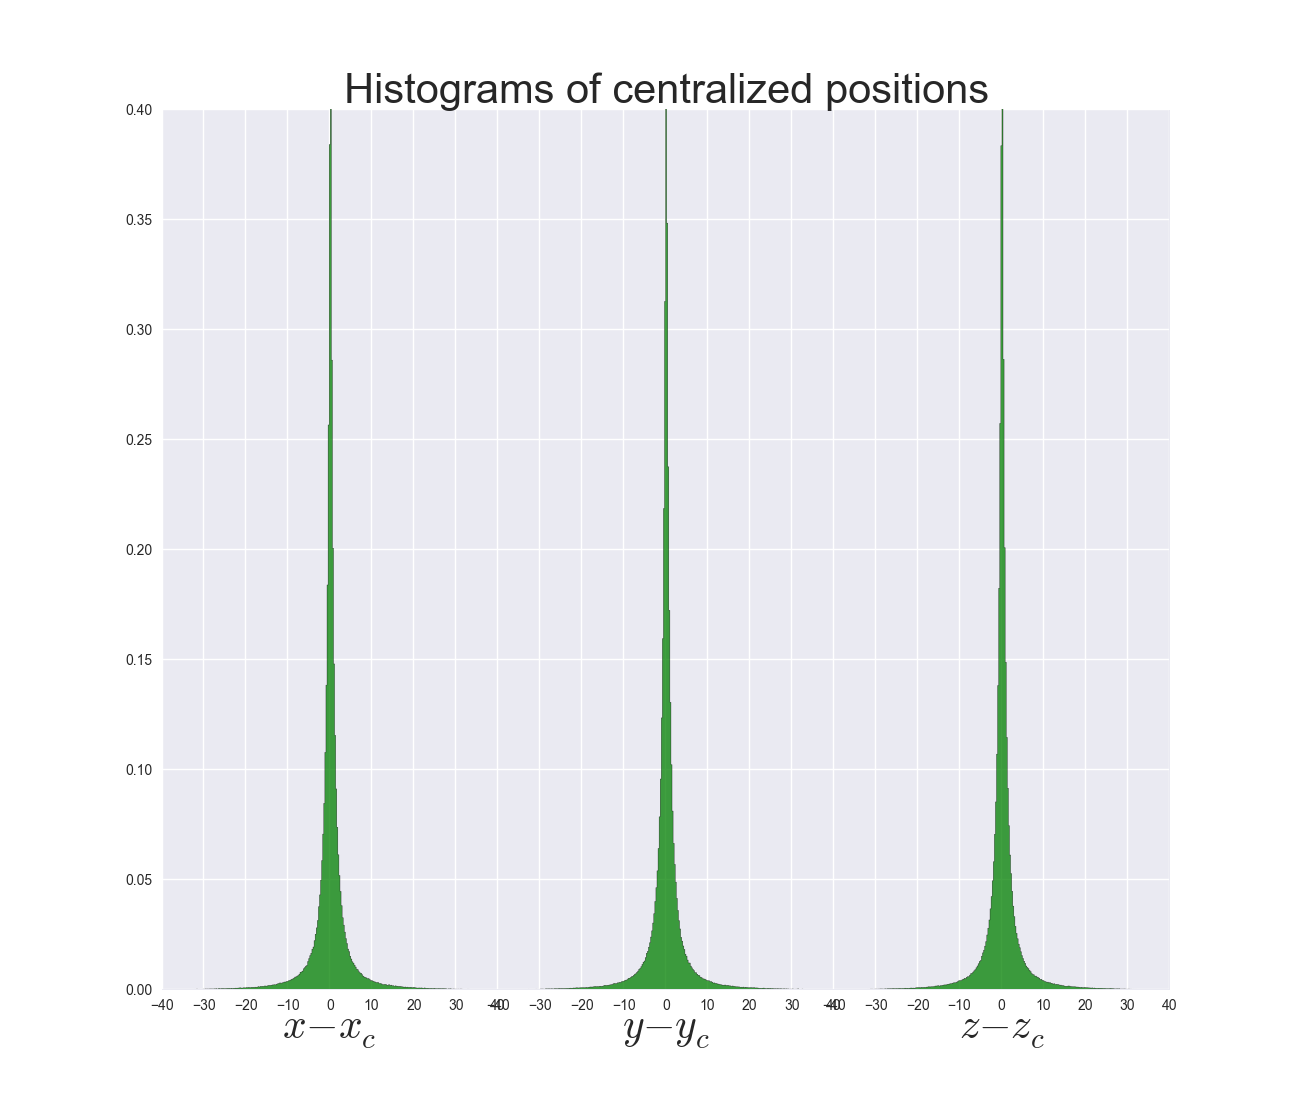
\includegraphics[width=1.0\linewidth]{img/Fig_x_hist.png}
\caption{All three cartesian coordinates are centralized around the halo center by subtraction of each individual particles position by the central coordinates $x_c$, $y_c$ and $z_c$.}
\label{fig:test}
\end{figure}

\textbf{Our Initial conditions are set up and ready to run. The next section introduces two principal ways to mimic the galaxy merger related effects. We will see how violent relaxation and phase mixing can be emulated by both sim. I and sim. II.}

\newpage
\section{Controlled numerical Simulations}
\textbf{Two different types of simulations are involved in this work, namely cosmological (see side projects in Appendix B) and controlled sims (described in this section). Both types are produced by using the GADGET-2 code (Springel 2005). The cosmological simulation is just analyzed, whereas the controlled simulations are both performed (inside a non-cosmological Newtonian box) and subsequently analyzed. By the name controlled it is meant that the sim. is more local and does not take an expanding spacetime into account. This enables a more detailed study where hierarchical clustering, mergers, build-up of halo sub-structure and accretion effects does not wash out the potential attractors of interest. The controlled sims is comprised of two types, namely I (An instantaneous change of the gravitational potential) and II (Energy exchange) which is further varied in four principal ways (cartesian, radial, tangential and total velocity perturbations).} \\ \\

\textit{When looking for universalities it is crucial to start from many different IC's. It is equally important to perturb these IC's in a variety of ways in order to make sure any found universalities is not an artifact of some artificial computer method. For this reason structures are subjected both to Sims. of type I and II. Both types have an underlying structure in common: Structures are perturbed and then gravity is allowed to work on them during subsequent simulation. This} perturbation$\rightarrow$simulation \textbf{method is kept under all numerical experiments in this work. They both serve to mimic the effects dominant during galaxy mergers since these dramatic events can alter characteristic features of the galaxies surrounding dark matter halos. It will then become more clear if these halos are driven towards any preferred state or configuration.} \\ \\

\centerline{\textbf{Particle number}} 
Particle number is steadily increased from $10^4$ to $10^5$ and finally all the way to $10^6$. To compute for example the velocity dispersion $\sigma$ or the density $\rho$ for a structure divided into 20 radial bins, and to get a good statistical result, $5\cdot 10^2$ particles is needed in each bin and therefore a minimum of $10^4$ particles must be included. However, in order to determine derived or constructed quantities such as $\kappa$ or $\gamma$, a minimum of $5\cdot 10^3$ particles in each of the 20 bins is more favorable and hence a total of $10^5$ particles is wanted. Looking at 2.nd order derivatives as for example in the project 'Bumpy road to universalities', even more particles must be included. A minimum of $5\cdot 10^4$ particles in each of the 20 bins is more favorable and hence a total of $10^6$ particles is wanted. \\

\centerline{\textbf{Gravitational softening}} 
For most cosmological simulations the softening depends upon the particle number in the following way [10]:
\begin{equation}
\epsilon \geq (\frac{3}{800\pi N^2})^{\frac{1}{3}}d  
\end{equation}
where d is the mean particle distance. For $N=5$, $\epsilon \geq \frac{1}{30}d$. For the controlled sims. it is simply assumed that $\epsilon$ scales as $N^{\frac{1}{3}}$. In Sparre and Hansens paper (\url{http://arxiv.org/abs/1210.2392}) a slightly smaller softening of 0.0050 were used in both the G-perturbations and the energy exchange simulations, It is therefore interesting to see if the attractor also exists if the above softening-values are used. This is expected to be the case, as a slightly larger softening only affects the very inner part. As a rule of thumb the softening must become 10 times larger when the particle number increases a thousand times [11]. \\ \\

\centerline{\textbf{Range of Jeans parameters}} 
For an Edd structure, $\beta = 0$ initially, and for an OM structure, $\beta \in [0,1]$. So the range of $\beta$ is set to $[0,1]$. For the density profile $\rho_{HQ}$, $\gamma \in [-3,-1]$, and for the density profile $\rho_{0,5}$, $\gamma \in [-5,0]$. The $\gamma$-range thus depends on the density profile under consideration.

\subsubsection{I: G-perturbations}
\textbf{To mimic the proces of violent relaxation during galaxy and cluster mergers this type of sim. creates an instantaneous change in the gravitational potential. Such a change perturbs the acceleration of each particle. This section gives a technical description of exactly how each structure was perturbed wrt the gravitational potential during this type of sim. The section gives an overview of a specific pattern of G-perturbations and following simulation, which is repeated a certain number of times, as well as an overview of the simulation times used during each step.} \\ \\

The purpose of the simulations of type I is to resemble the proces of violent relaxation during mergers. But instead of using the relation describing violent relaxation $\big(\frac{dE}{dt} = \frac{d\Phi}{dt}\big)$, where a time-dependence of the gravitational potential ($\Phi$) exists, a time variation of Newtons gravitational constant is applied, G(t). This effectively produces the same effect. After each perturbation of G from its standard value, the structures are simulated. This pattern continues for a certain amount of time until a new stable configuration is found. Practically, changes are made to the value of Newtons gravitational constant G from its standard value of $G = 6.67 \cdot 10^{-11} \frac{Nm^2}{kg^2}$ here corresponding to $G=1$ in non-SI units, to either 1.2 or 0.8 times the standard value, corresponding to an increase or decrease by 20 \%, or 1.05 to 0.95 times the standard value, corresponding to an increase or decrease by 5 \%. Either 20 or 5 pct is added or subtracted systematically from G in a certain pattern (see table 3). The Simulations always start out with $G = 1$ in Run 0 which last for 100 simulation times. This is done to give the structure time to work under its own gravity and make sure the IC's are set up correctly. It provides a way to see that the IC is in a stable configuration. The pattern from Run 1 to Run 5 is then repeated a certain number of times (see table 4). Ending up with runs of $G=1$ for longer time gives the structures better chance to reach stable equilibria (see tables 5-7). The idea behind changing the G-value by a smaller amount (5 pct.) from the standard value (as is the case with sim B) is to have the structure depart less from equilibrium during the simulations. It is seen later on in the analysis of the velocity distribution functions that these are not so different if the perturbations are larger or smaller, but the $\gamma$ vs. $\beta$ and $\gamma + \kappa$ vs. $\beta$ plots look slightly different if G is perturbed by 20\% or by 5\%. GADGET-2 makes a certain number of runs with varying values assigned to the gravitational constant G (Corresponding to perturbing the gravitational potential, i.e. An instantaneous change in $\Phi$ ). Most of these runs each produce 6 snapshot files, except for the last run in each simulation, where the time is increased from Timemax = 100 to Timemax = 2300 (giving 93 snapshots). The method of varying the potential corresponds to changing the accelerations of the individual particles. It is then interesting to see how the structures will respond, more on this in the next section: 'The attractor'. When the gravitational constant is lowered to the value of $ G = 0.8 $ and a structure is simulated by Gadget-2 for 100 time units, an expansion of that structure naturally occurs. When the gravitational constant is raised to the value of $ G = 1.2 $ and the structure again is simulated for 100 time units, A contraction of this structure now happens. This type of simulation where the structure pulsates is reminiscent of violent relaxation. \\ \\

\begin{table}[!htbp]
\centering
\begin{tabular}{|c|c|c|c|c|}
\hline
 Simulation    & A, $C_4$-$C_6$, $CS_4$-$CS_6$, $D_1$, $D_2$ and $DS_1$ & B          \\ \hline
 Run No.       &   G-value                                              &   G-value  \\ \hline
 0			   &     1.0                 						       &     1.0    \\ \hline
 1			   &     1.2    											   &     1.05   \\ \hline
 2			   &     0.8     										   &     0.95   \\ \hline
 3			   &     1.0   											   &     1.0    \\ \hline
 4			   & 	 1.0     										   &     1.0    \\ \hline
 5			   & 	 1.0     									       &     1.0    \\ \hline
\end{tabular}
\caption {Simulation I pattern. First this table states the name of each structure. The B structure is placed alone as it has a unique percentage of change to G of only $5 \%$, whereas the others all have G-perturbations to the order of $20 \%$. For each run a simulation time of 100 is used (corresponding to one dynamical time at $r=12.7r_s$). Left column numerates the different simulation runs. For all structures undergoing this type of simulation they are initially set up in the GADGET-2 code to be subjected to gravity with a potential corresponding to the standard value of G (here it means G=1). After the zeroth run  the simulation is paused and an increase of the G value (corresponding to a stronger gravitational potential) is applied, after which the simulation is continued. After the next 100 simulation times the G value is decreased (corresponding to a weaker potential) and the simulation is allowed to continue yet again for the next 100 simulation times. Finally G remains at the standard value for $3\cdot 100$ simulation times. This whole pattern or 'chunk' from run 1 to run 5 is then repeated a different number of times which can be seen in the following table.
}
\end{table}

\begin{table}[!htbp]
\centering
\begin{tabular}{|c|c|c|c|c|}
\hline
 Simulation                   & A & B and E & $C_4$-$C_6$ and $CS_4$-$CS_6$ & $D_1$, $D_2$ and $DS_1$ \\ \hline
 No. repetitions of pattern   & 9 & 39& 9 & 9 \\ \hline
\end{tabular}
\caption {Pattern repetitions. The 'chunks' of G-perturbations and subsequent simulations are repeated for the above stated number of times for all the different structures in question.}
\end{table}

\begin{table}[!htbp]
\centering
\begin{tabular}{|c|c|c|}
\hline
            & Simulation A, $C_4$-$C_6$ and $CS_4$-$CS_6$ &             \\ \hline
 Run        &     G                                       &  TimeMax    \\ \hline
 46         &    1.2                                      &    100      \\ \hline
 47         &    0.8                                      &    100      \\ \hline
 48         &    1.0                                      &    2300     \\ \hline   
\end{tabular}
\caption {Final runs. After the series of pattern repetitions shown before, for the here mentioned structures three final \textit{perturbation} $\rightarrow$ \textit{simulation} experiments are run: G is increased by $20 \%$ and structures are subjected to their self-gravity for 100 sim. times, G is decreased by $20 \%$ and structures are run for 100 sim. times and finally G is kept at unity and structures are run for 2300 sim. times in order to give the outer part of the structures more time to reach stable equilibria.}
\end{table}

\begin{table}[!htbp]
\centering
\begin{tabular}{|c|c|c|}
\hline
            & Simulation B and E &             \\ \hline
 Run        &     G              &  TimeMax    \\ \hline
 196        &    1.05            &    100      \\ \hline
 197        &    0.95            &    100      \\ \hline
 198        &    1.0             &    2300     \\ \hline   
 199        &    1.0             &    2300     \\ \hline  
\end{tabular}
\caption {Final runs. After the series of pattern repetitions shown before, for the here mentioned structures three final \textit{perturbation} $\rightarrow$ \textit{simulation} experiments are run: G is increased by $5 \%$ and structures are subjected to their self-gravity for 100 sim. times, G is decreased by $5 \%$ and structures are run for 100 sim. times and finally G is kept at unity and structures are run for $2\cdot 2300$ sim. times}
\end{table}

\begin{table}[!htbp]
\centering
\begin{tabular}{|c|c|c|}
\hline
            & Simulation $D_1$, $D_2$ and $DS_1$ &             \\ \hline
 Run        &     G                              &  TimeMax    \\ \hline
 49         &    1.0                             &    2300     \\ \hline   
\end{tabular}
\caption {Final run. After the series of pattern repetitions shown before, for the here mentioned structures one final \textit{perturbation} $\rightarrow$ \textit{simulation} experiments is run: G is kept at unity and the structures are run for 2300 sim. times}
\end{table}

\centerline{\textbf{Particle tracking}}
In order to test whether or not structures subjected to Sim. I has the tendency to expand systematically in the central region and throw out particles when pulsating as the effect of changing the gravitational potential, a few test particles has been chosen and tracked through a few different time-slices/snapshot-files of the simulations (See figure 10). In conclusion, there is no major systematic tendency of outward drift but only a small effect of turning initial cuspy profiles into profiles with small cores.

\begin{figure}[!htbp]
\centering
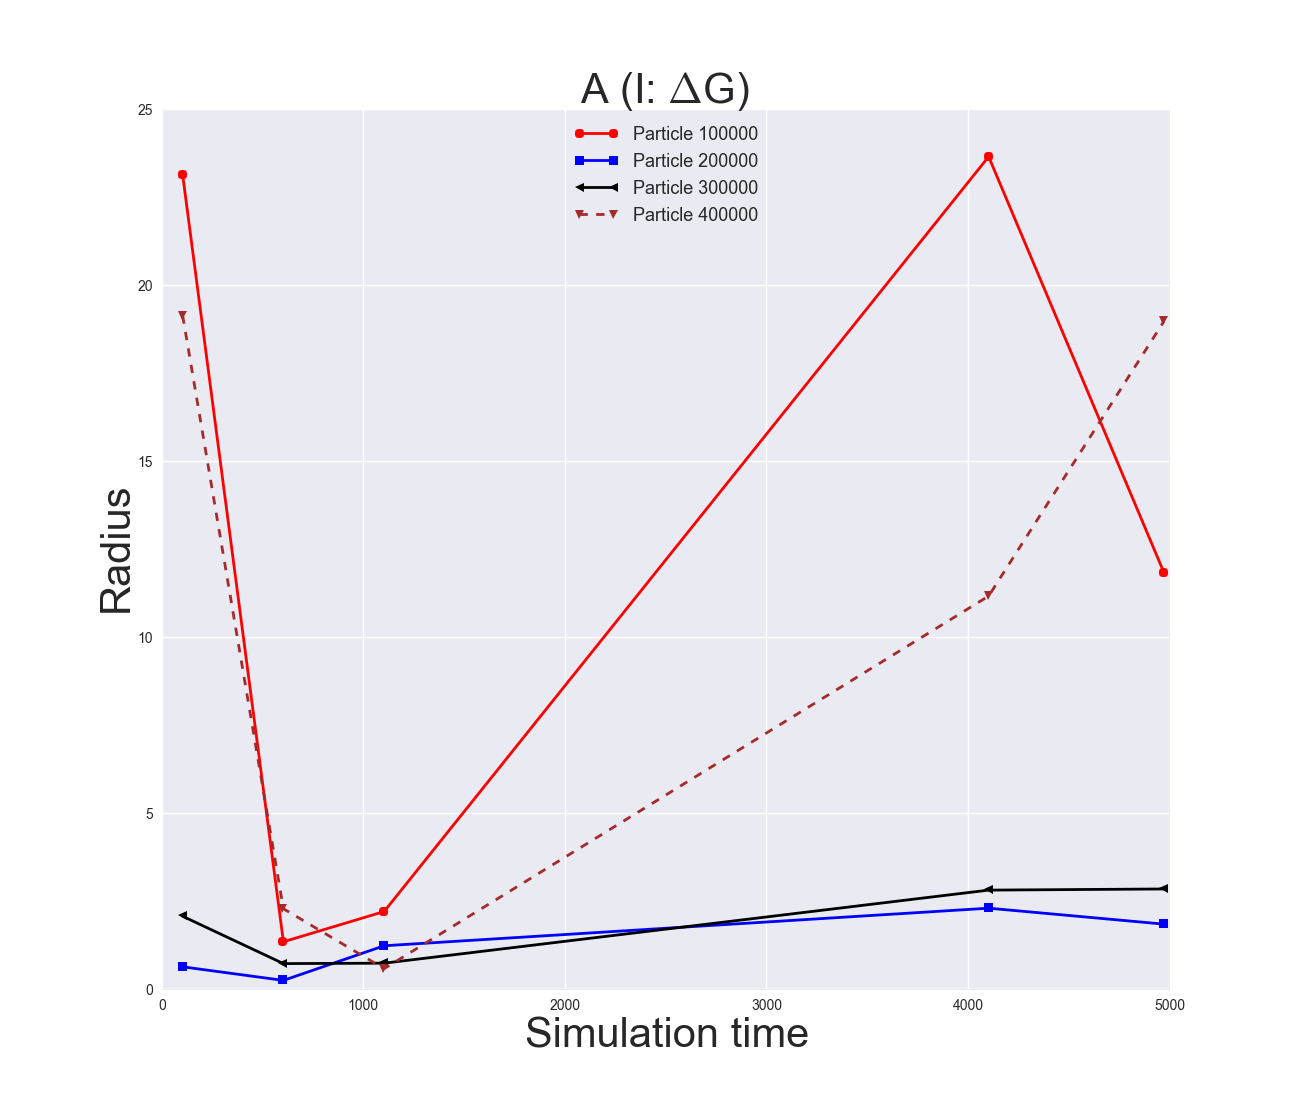
\includegraphics[width=1.0\linewidth]{img/Fig_combine_ASCII_A.png}
\caption{Time evolution of radius for a few chosen particles (ID's $10^5$, $2\cdot10^5$, $3\cdot10^5$ and $4\cdot10^5$) is plotted for selected snapshot files (IC, 5$\_$005, 10$\_$005, 40$\_$005 and 48$\_$009) of Sim. I for structure A. The figure shows that there is no systematic tendency of neither outward nor inward drift as indicated by all four particles changing radius in a stochastic manner as time evolves. This is expected due to the pulsating effect the G-perturbations has on structures.}
\label{fig:test}
\end{figure}

\centerline{\textbf{Total velocity profile}} 
As all structures have a scale-radius of unity, $r_s = 1$, the total velocity distribution is centered around unity as well (See figure 11). Over time however, substructure is created as we notice the emergence of filaments or 'fingers', each finger corresponding to an increase in the gravitational potential thus increasing individual particle accelerations and their contribution to the overall total velocity distribution is to drift outwards towards larger radii in this characteristic filament pattern. (see figure 12 and 13). 

\centerline{\textbf{Final density}} 
Figure 14 shows the flattening of structures as their density profiles go from cuspy to cored over the duration of the simulations. Final structures in average have cores with a size of $\log \frac{r}{r_{-2}} = -0.5$, i.e. $\frac{r}{r_{-2}} \approx 0.32$ or put in other words the cores span 32 \% of $r_{-2}$, the radius where $\gamma = -2$ (for a HQ profile this equals the scale radius, $r_{-2} = r_s$). \\
\centerline{\textbf{Structures become anisotropic over time}} \\
In figure 15 the effect this sim. type I has on velocity anisotropy can be seen. All structures will over time grow radially biased wrt. the $\beta$-profile no matter if they belong to Edd or OM ICs. \\
\centerline{\textbf{Density slope extremas}} \\
Figure 16 reveals an interesting feature of final $\gamma$ shapes. notice in the outer part how there seem to be distinct bumps and wiggles. This is explored further in the side project found in App. B.4 'The bumpy road to universalities' where different normalizations are carried out to look for universalities in the final $\gamma$-profiles which seem to poses up to 6 unique local extremas (3 minima and 3 maxima). \\
\centerline{\textit{Evolution of radial velocity dispersion}} \\
Figure 17 compares initial and final $\kappa$-profiles. Particularly the two larger structures A and B both with $N = 10^6$ particles have spread out into a larger area. This indicates an increase of the radial velocity dispersion which is the result of the pulsating  that structures undergo during these acceleration perturbations. that effect is much more visible in a large structure holding more particles, as these have better statistics to give a more complete look of the radial velocity spread. 

\begin{figure}[!htbp]
\centering
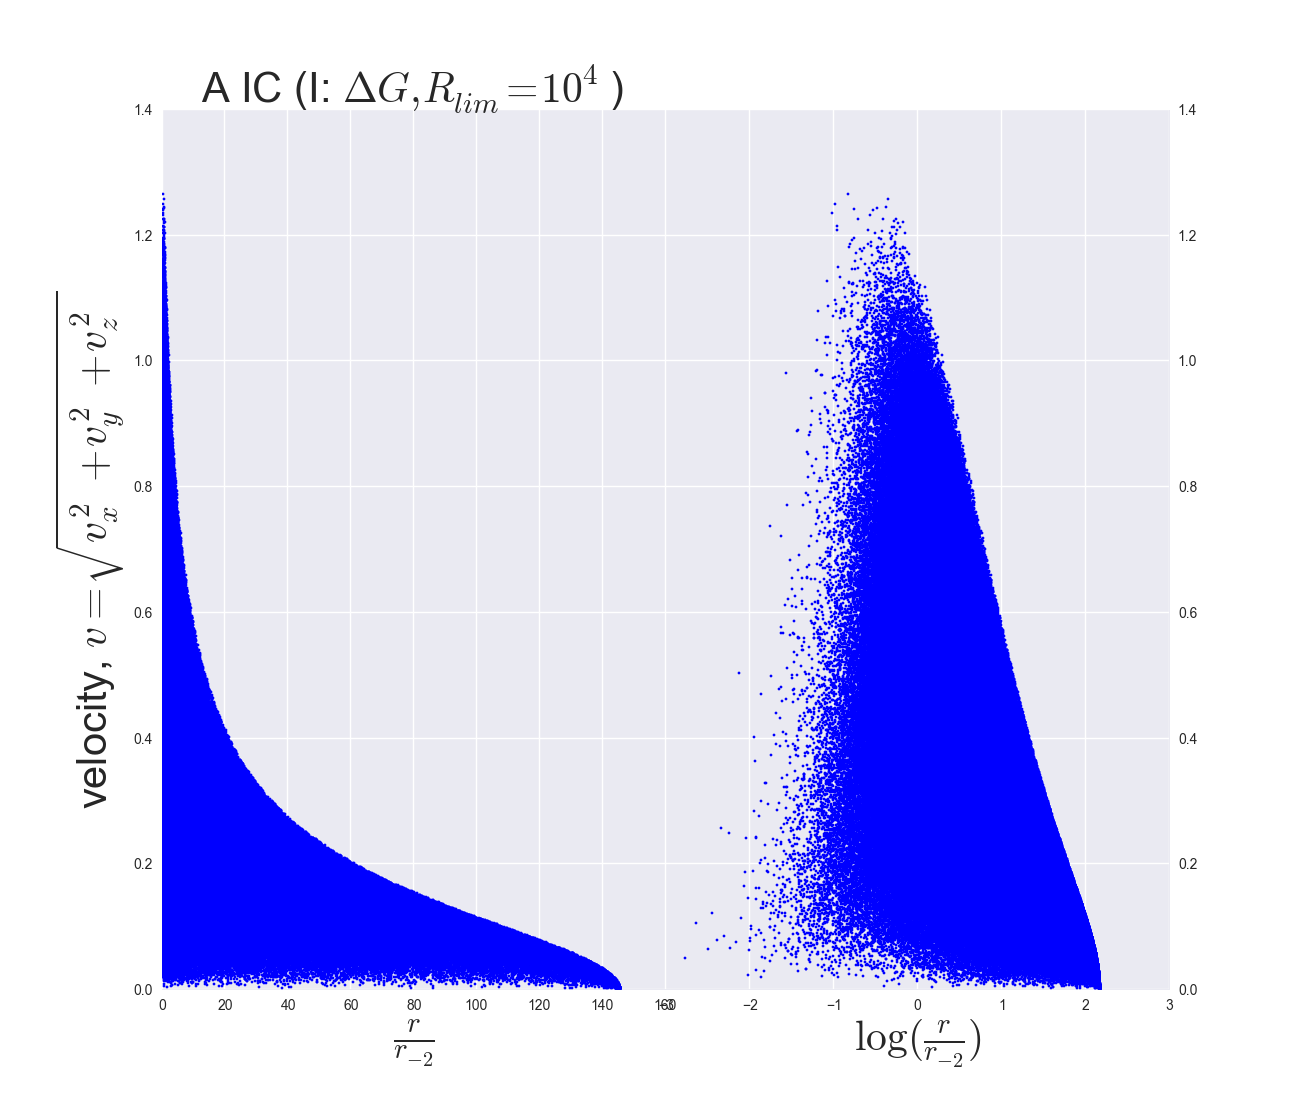
\includegraphics[width=1.0\linewidth]{img/A_IC_v_logr_r2.png}
\caption{Plot of $v_{tot}$ vs. $\frac{r}{r_{-2}}$ and $\log (\frac{r}{r_{-2}})$ respectively for IC of A. Analyzed out to a radius of $R_{lim} = 10^4$. Notice how the majority of particles are clustered around the value $\log (\frac{r}{r_{-2}}) = 0$.}
\label{fig:test}
\end{figure}

\begin{figure}[!htbp]
\centering
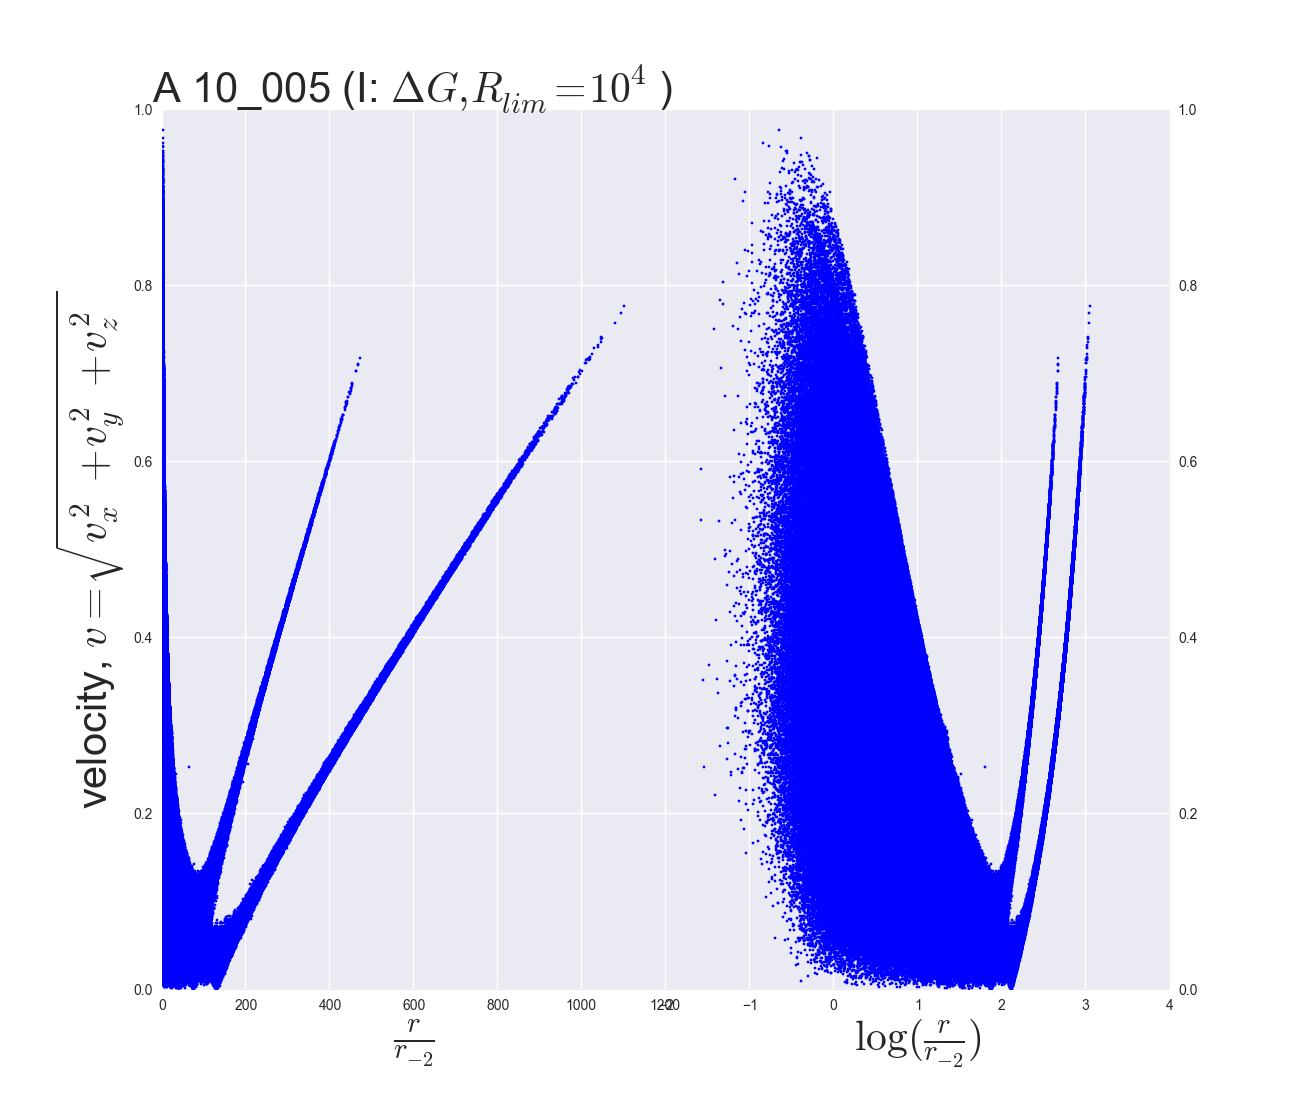
\includegraphics[width=1.0\linewidth]{img/A_10_005_v_logr_r2.png}
\caption{$v_{tot}$ vs. $\frac{r}{r_{-2}}$ and $\log (\frac{r}{r_{-2}})$ respectively for sim. I of structure A, after 1100 simulation timesteps (corresponding to $11\cdot t_{dyn}$ at $r=13.7\cdot r_s$). Analyzed out to a radius of $R_{lim} = 10^4$. A very slight shift of the main part of the structure towards larger radii is seen. Two velocity 'fingers' or velocity filaments can now be seen at larger radii. They are a direct response to the perturbation where $\Phi$ is first increased and then decreased due to a change in Newtons gravitational constant. This greatly increase particles velocities at large radii, forcing some of them to become gravitationally unbound. Two segments of 'G-chunks' have thus been run up to this stage as can be seen from simply counting the velocity filaments}
\label{fig:test}
\end{figure}

\begin{figure}[!htbp]
\centering
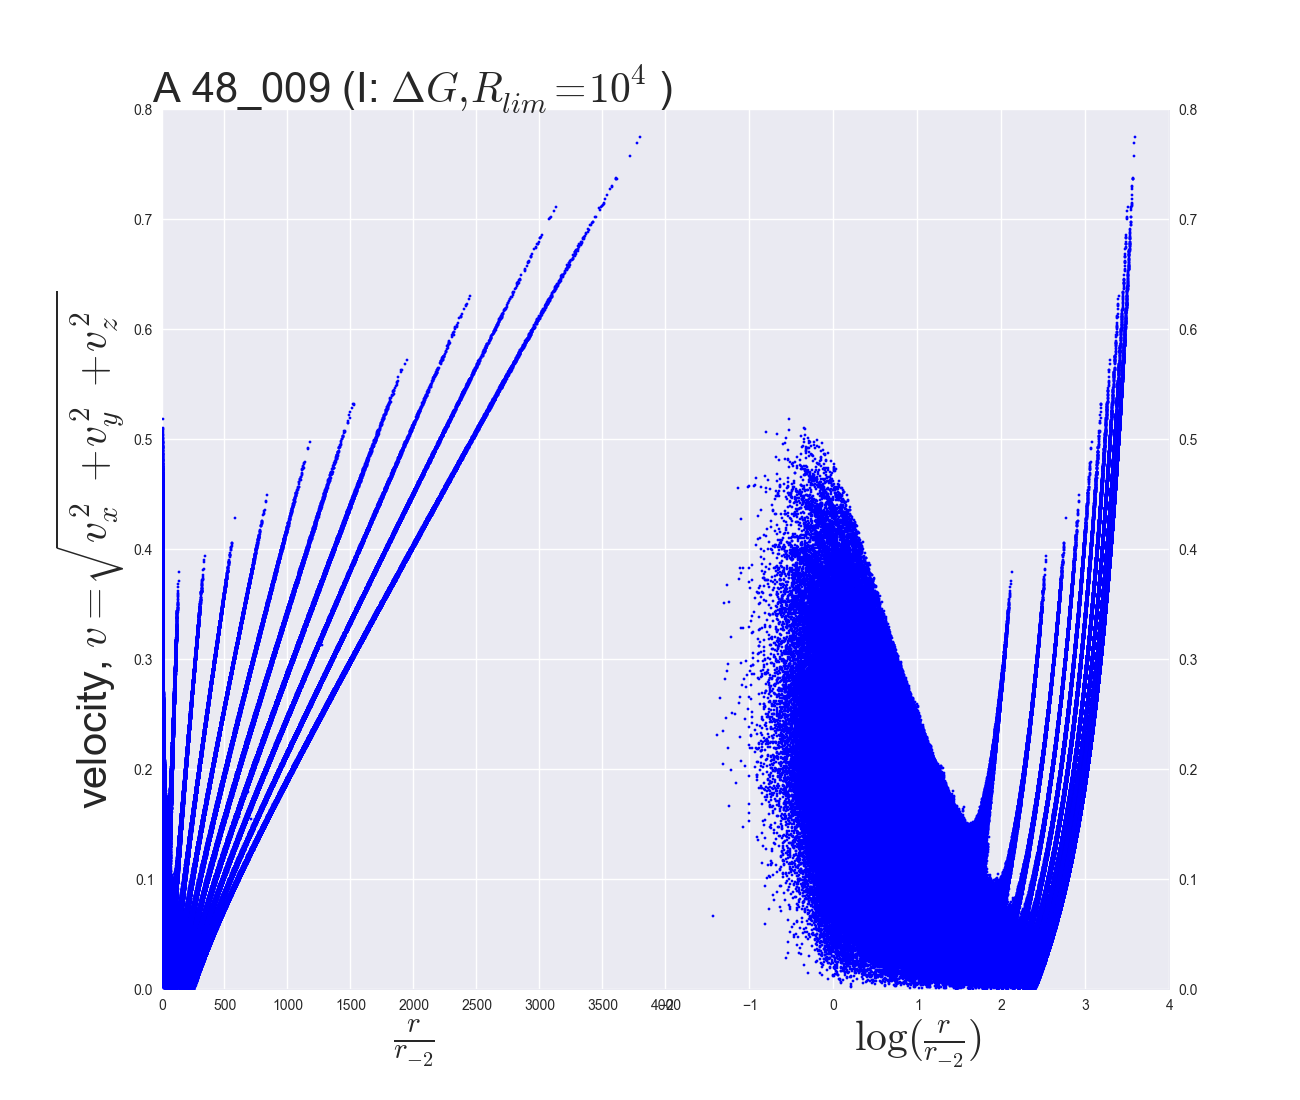
\includegraphics[width=1.0\linewidth]{img/A_48_009_v_logr_r2.png}
\caption{$v_{tot}$ vs. $\frac{r}{r_{-2}}$ and $\log (\frac{r}{r_{-2}})$ respectively for sim. I of structure A, after 4970 simulation timesteps (corresponding to $49.7\cdot t_{dyn}$ at $r=13.7\cdot r_s$). Analyzed out to a radius of $R_{lim} = 10^4$. The shifting of the main part of the structure towards larger radii remains present but is still not very significant. A much larger time span between this figure and the previous of $\Delta t_{sim} = 4970-1100 = 3870$ (or $38.7\cdot t_{dyn}$ at $r=13.7\cdot r_s$) means that far more 'G-chunks' have been run at this stage, in fact ten of them, and again counting the velocity filaments we see this to be illustrated by the existence of ten filaments.}
\label{fig:test}
\end{figure}

\begin{figure}[!htbp]
\centering
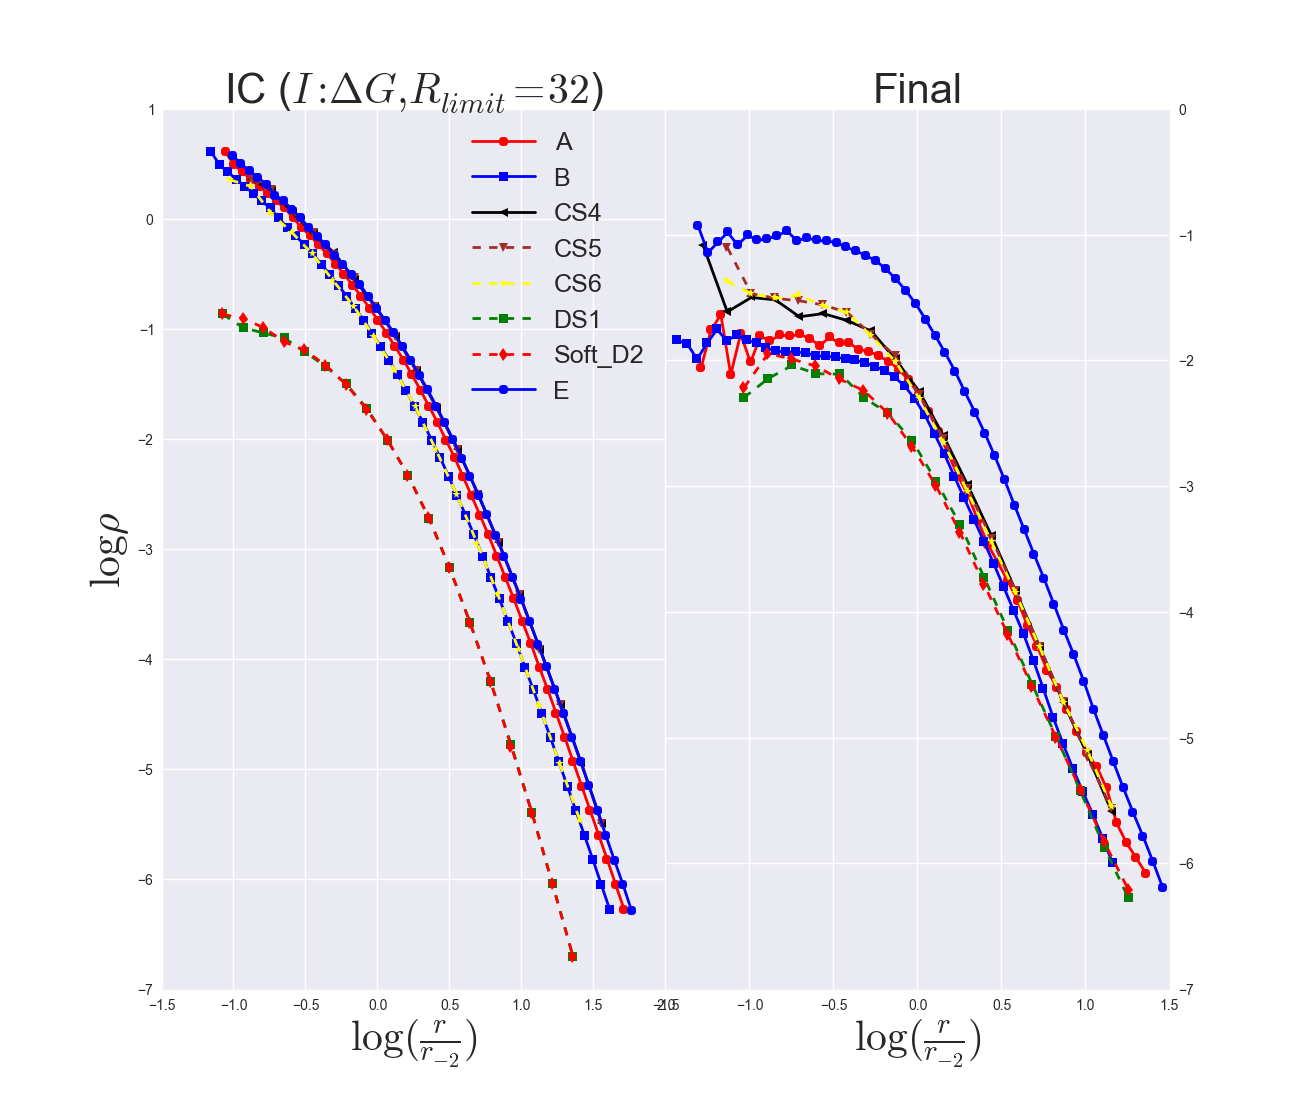
\includegraphics[width=1.0\linewidth]{img/log_r_r2_rho_IC_Final_R32.png}
\caption{$\rho$ vs. $\log (\frac{r}{r_{-2}})$. The IC profiles are all cuspy (apart from the DS1 and Soft$\_$D2 structures which have unique density profiles with inner and outer slope zero and minus 5 respectively); i.e. their inner density profiles are very steep. As time evolves all profiles develop small cores in the very inner region. This can be easily understood through some simple dynamical arguments; Consider the few central particles that just happens to have a very high velocity greater than the escape velocity of the halo. Increasing the gravitational potential and then letting the simulation run will make these central particles travel outwards as the now stronger potential will tend to on average pull the particles into, and through the center (as they do not experience any collisions). Once through the center their travel continues out to large radii from there they will move with constant speed away from the structure forever. Hence the catchphrase 'Once out, always out' applies to these high velocity central particles. This can be thought of as the main reason for the flattening of initially cuspy or steep density profiles at small radii. Structures with $N = 10^6$ particles (A, B and E) are divided into 50 bins which are logarithmic in radius, whereas structures with $N = 10^5$ particles are divided into just 20 bins to ensure a sufficient number of particles in each bin. The structures are cut off at a radius of $R_{lim} = 32\cdot r_s$ corresponding to the $log_{10}$ value of 1.5}
\label{fig:test}
\end{figure}

\begin{figure}[!htbp]
\centering
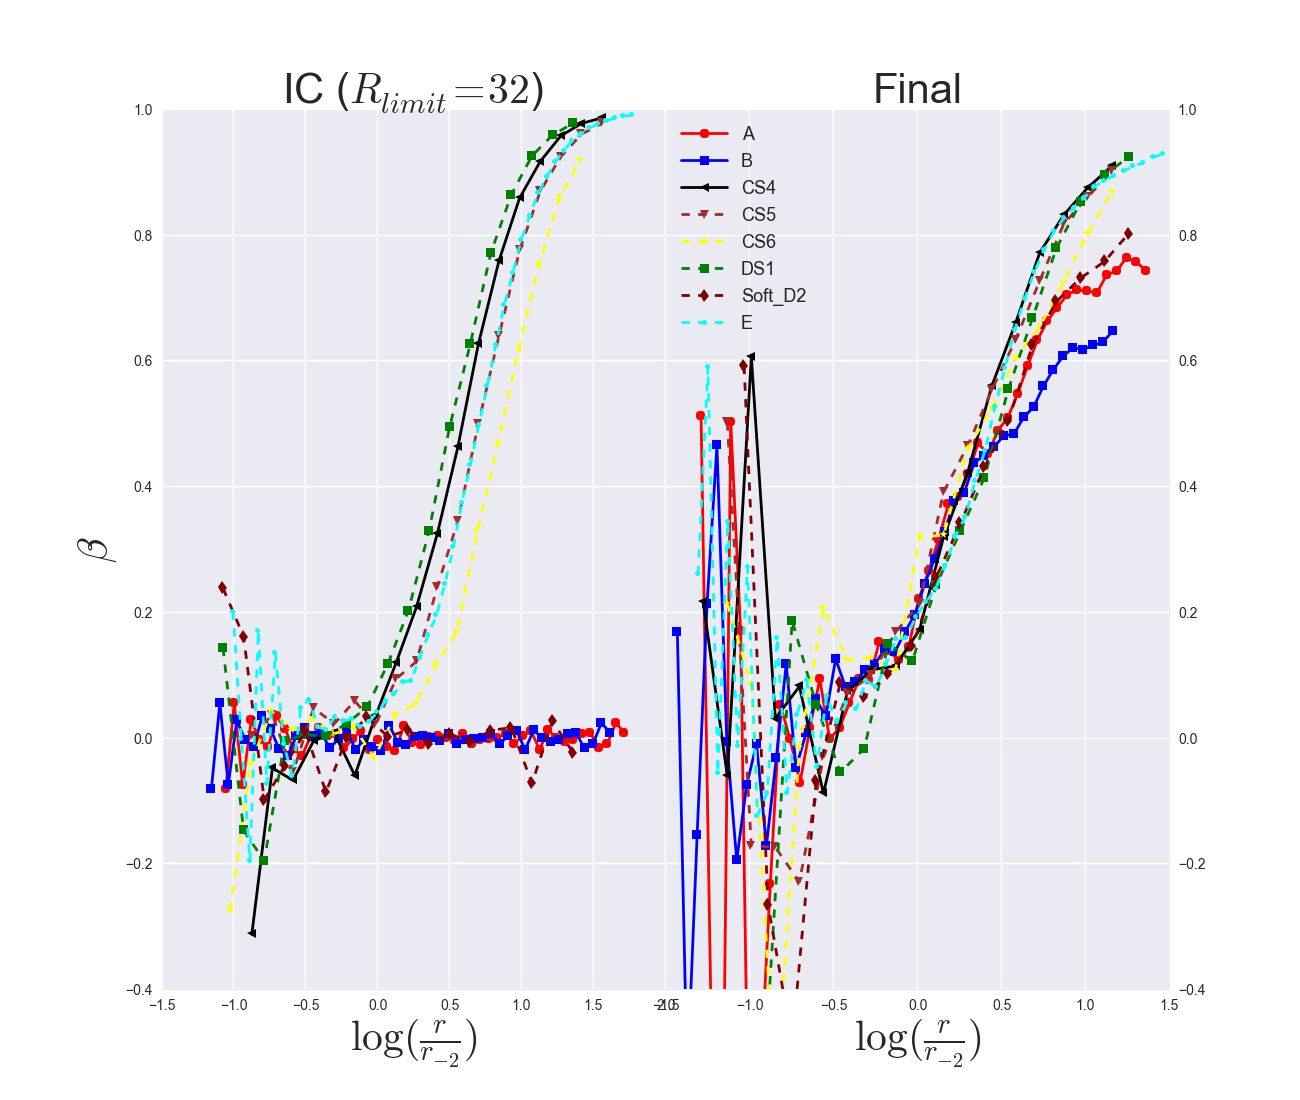
\includegraphics[width=1.0\linewidth]{img/Fig_logr_r2_beta_ABCS4CS5CS6DS1D2E_IC_Final_R_limit_32.png}
\caption{$\beta$ vs. $\log (\frac{r}{r_{-2}})$. By comparing IC with final products wrt the velocity anisotropy parameter $\beta$ it is seen that structures which are initially isotropic (A, B and Soft$\_$D2, created by Eddingtons inversion method) become radially biased over time and the structures with initial velocity anisotropy (CS4, CS5, CS6, DS1 and E, which are OM models) remain anisotropic in the outer part as time goes. The inner part of the final structures are dominated by large fluctuations due to Poisson noise and it is therefore not possible to say anything about this region for certain apart from the fact that the fluctuations are centered around $\beta = 0$ so the structures could be ergodic in the inner part. The span in the $\beta$ parameter for IC and final products are approximately $[-0.2;1.0]$, which can also be seen later in the ($\beta$,$\gamma$)- and ($\beta$,$\gamma + \kappa$)- plots. Structures with $N = 10^6$ particles (A, B and E) are divided into 50 bins which are logarithmic in radius, whereas structures with $N = 10^5$ particles are divided into just 20 bins to ensure a sufficient number of particles in each bin. The structures are cut off at a radius of $R_{lim} = 32\cdot r_s$ corresponding to the $log_{10}$ value of 1.5}
\label{fig:test}
\end{figure}

\begin{figure}[!htbp]
\centering
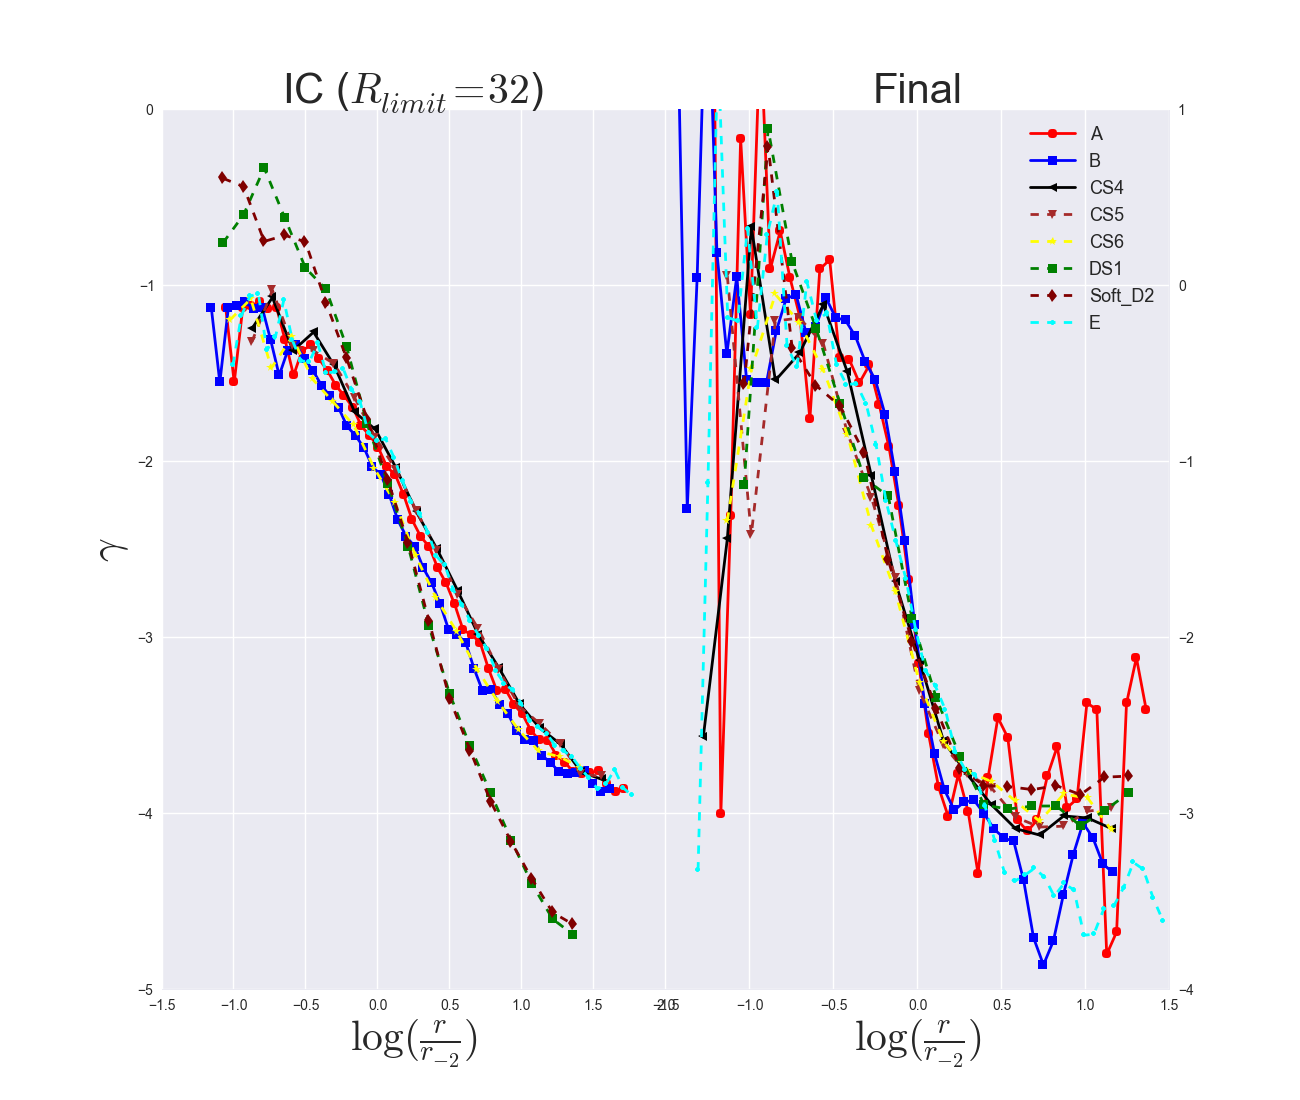
\includegraphics[width=1.0\linewidth]{img/Fig_logr_r2_gamma_ABCS4CS5CS6DS1D2E_IC_Final_R_limit_32.png}
\caption{$\gamma$ vs. $\log (\frac{r}{r_{-2}})$. Structures with $N = 10^6$ particles (A, B and E) are divided into 50 bins which are logarithmic in radius, whereas structures with $N = 10^5$ particles are divided into just 20 bins to ensure a sufficient number of particles in each bin. The structures are cut off at a radius of $R_{lim} = 32\cdot r_s$ corresponding to the $log_{10}$ value of 1.5}
\label{fig:test}
\end{figure}

\begin{figure}[!htbp]
\centering
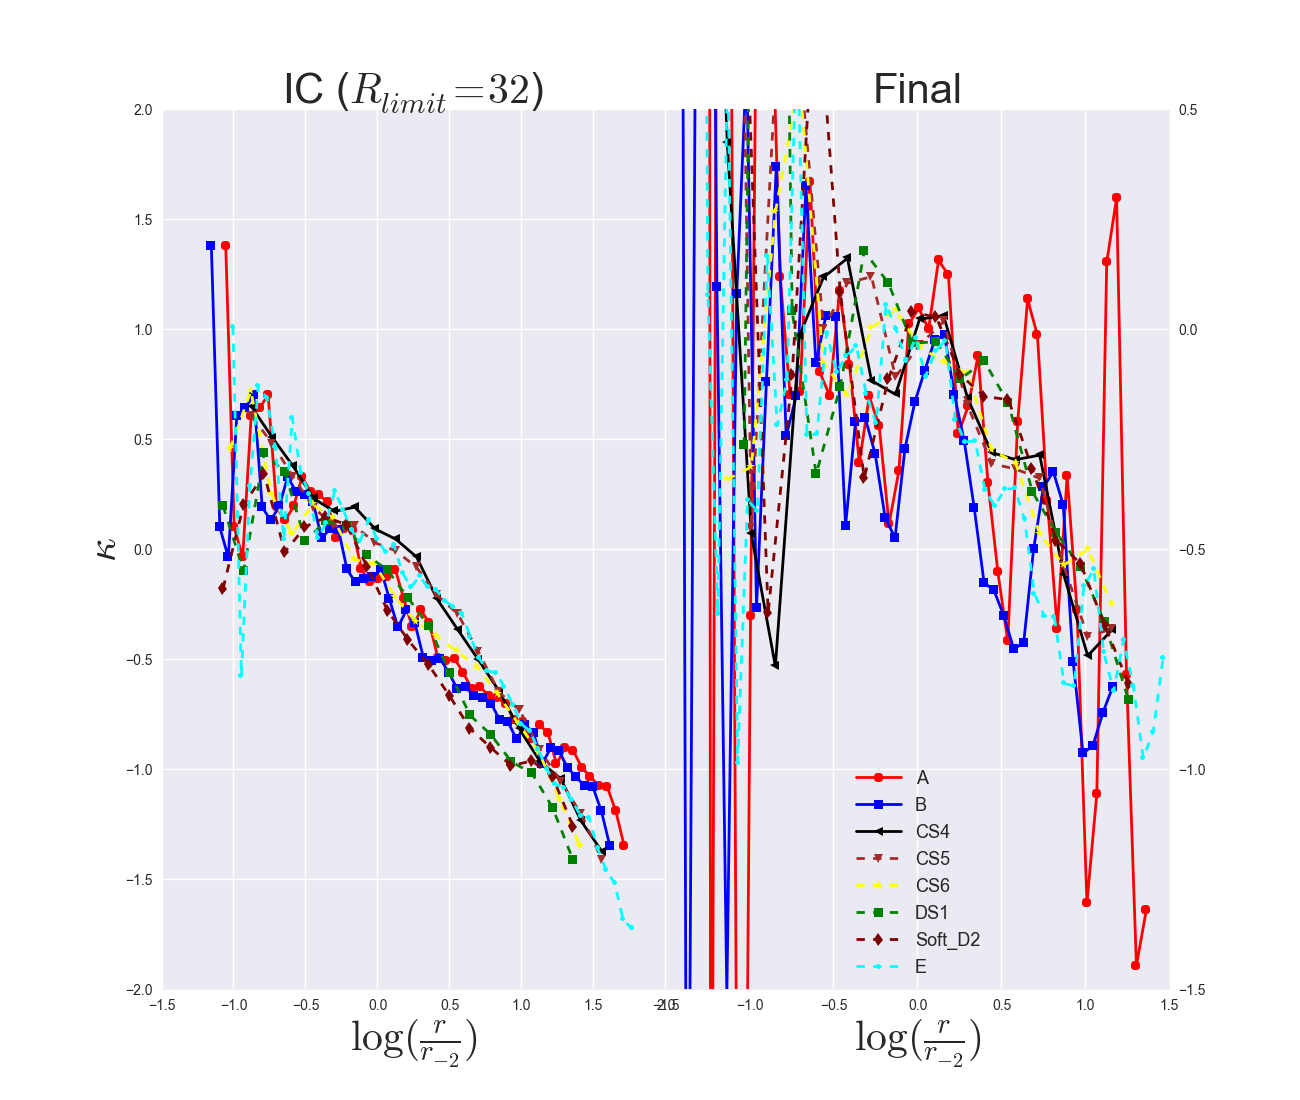
\includegraphics[width=1.0\linewidth]{img/Fig_logr_r2_kappa_ABCS4CS5CS6DS1D2E_IC_Final_R_limit_32.png}
\caption{$\kappa$ vs. $\log (\frac{r}{r_{-2}})$. Structures with $N = 10^6$ particles (A, B and E) are divided into 50 bins which are logarithmic in radius, whereas structures with $N = 10^5$ particles are divided into just 20 bins to ensure a sufficient number of particles in each bin. The structures are cut off at a radius of $R_{lim} = 32\cdot r_s$ corresponding to the $log_{10}$ value of 1.5}
\label{fig:test}
\end{figure}






\begin{figure}[!htbp]
\centering
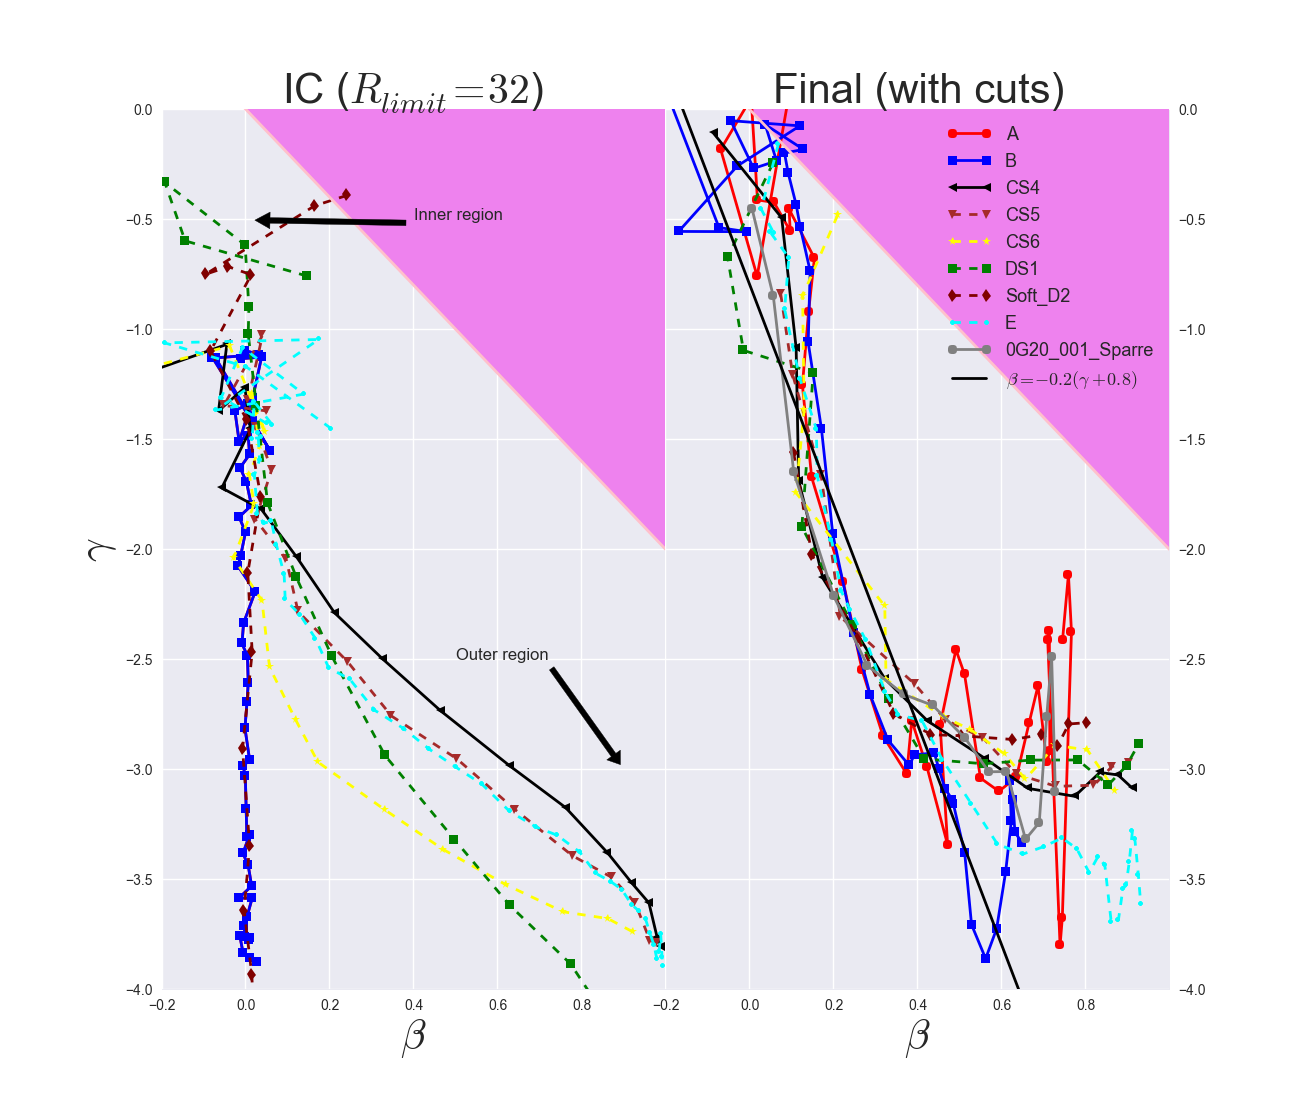
\includegraphics[width=1.0\linewidth]{img/Fig_beta_gamma_ABCS4CS5CS6DS1D2E_IC_Final_R_limit_32.png}
\caption{$\gamma$ vs. $\beta$. Left panel shows the initial conditions and right panel the final products after sim. I of structures A, B, $CS_4$, $CS_5$, $CS_6$, $DS_1$, $D_2$ and E. Notice how the IC spans a large volume of the Jeans parameter space whereas the final products are attracted to a 1-dimensional s-shaped attractor curve which effectively reproduces results found by others [4]. This attractor can be described analytically as $\gamma + \kappa = -8\beta $ for the inner part and $\gamma + \kappa = -0.7-4\beta $ for the outer region. For reference the final structures are plotted together with the linear relation found by Hansen and Moore (solid black line, $ \beta = -0.2(\gamma + 0.8)$) as well as data from [4] which are in very good agreement.}
\label{fig:test}
\end{figure}

\begin{figure}[!htbp]
\centering
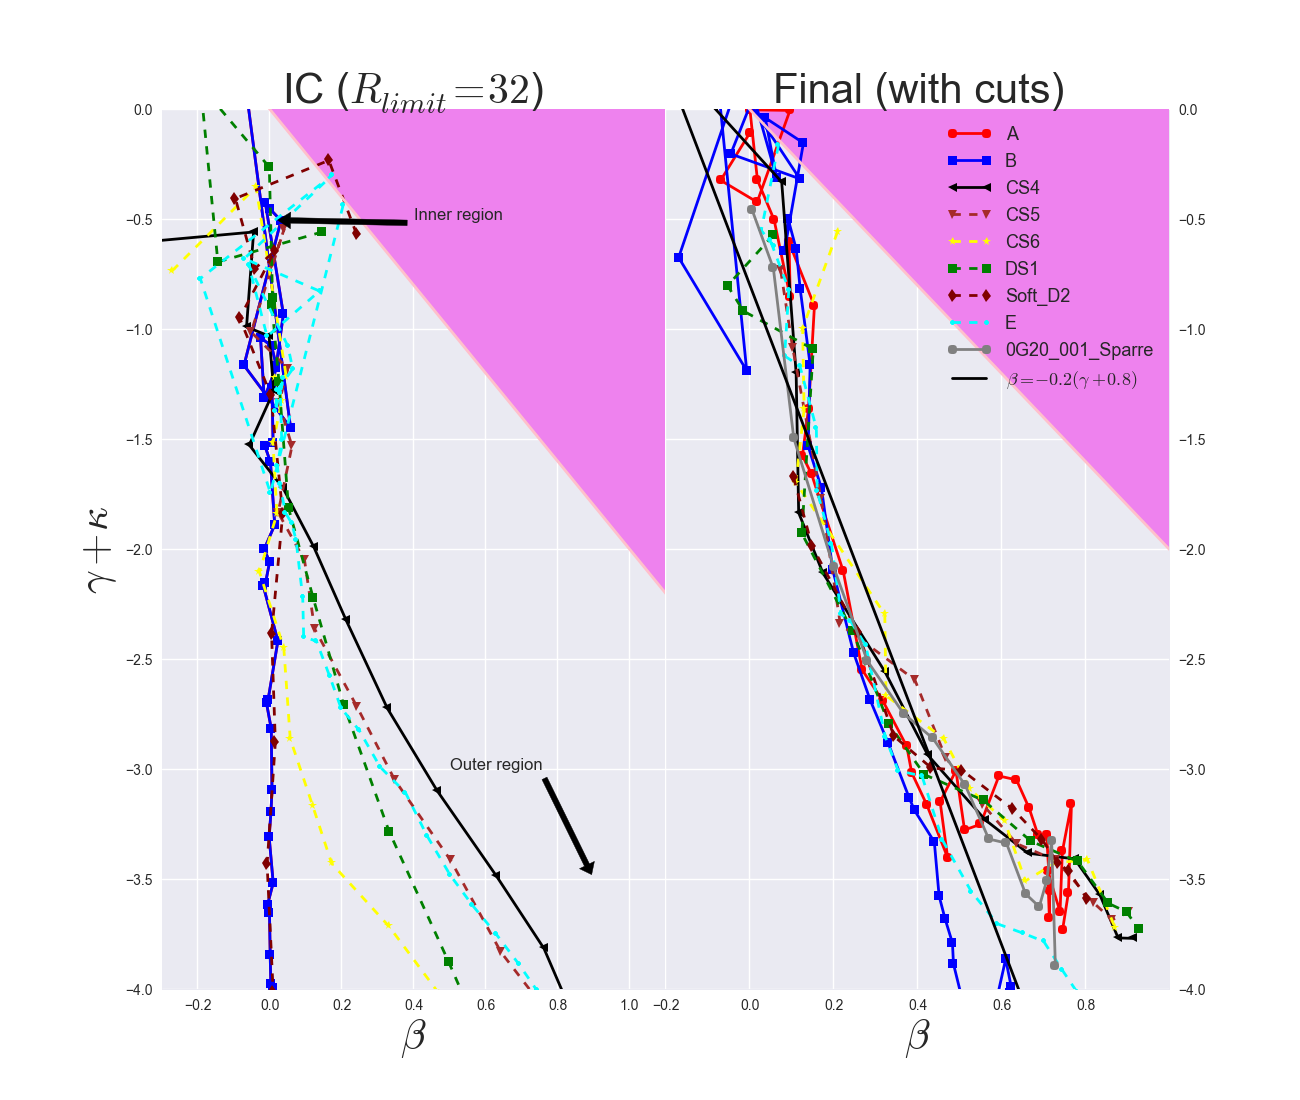
\includegraphics[width=1.0\linewidth]{img/Fig_beta_gamma_kappa_ABCS4CS5CS6DS1D2E_IC_Final_R_limit_32.png}
\caption{$\gamma + \kappa$ vs. $\beta$. Left panel shows the initial conditions and right panel the final products after sim. I of structures A, B, $CS_4$, $CS_5$, $CS_6$, $DS_1$, $D_2$ and E. Notice how the IC spans a large volume of the Jeans parameter space whereas the final products are attracted to a 1-dimensional s-shaped attractor curve which effectively reproduces results found by others [4]. This attractor can be described analytically as $\gamma + \kappa = -8\beta $ for the inner part and $\gamma + \kappa = -0.7-4\beta $ for the outer region. For reference the final structures are plotted together with the linear relation found by Hansen and Moore (solid black line, $ \beta = -0.2(\gamma + 0.8)$) as well as data from [4] which are in very good agreement.}
\label{fig:test}
\end{figure}

\subsubsection{IIa: Energy exchange (cartesian velocity perturbations)}
\textbf{Using structures holding a variety of initial conditions, this simulation type mimics effects found in galaxy mergers. Specifically, for all of these structures (named as $B$, $CS_4$, $CS_5$, $CS_6$, $DS_1$, $D_2$ and $E$) the total velocities inside spherical bins is perturbed for each of its particles by multiplying each of those given particles cartesian velocities ($v_x$, $v_y$ and $v_z$) by random numbers in different ranges, firstly the range $[0.8, 1.2]$ (corresponding to perturbing the kinetic energies by random numbers in the range $\frac{1}{2}\cdot[0.64, 1.44]$), taken from the continuous uniform distribution. This is a symmetric probability distribution where all intervals of the same length between 0.8 and 1.2 are equally probable. Following this exchange of kinetic energies between particles in fixed spherical bins, a normalization factor is applied to the total velocities, which ensures energy conservation. After such a velocity 'kick' the structures are simulated under their self gravity allowing them to flow a bit under their new velocities. This procedure is then repeated for a total of 40 runs (with one initial run where there is no perturbation. This allows the OM models to reach equilibrium, as they are not perfectly equilibrated when set up as OM models. It is done for Edd structures as well to be certain of equilibrium before any perturbations take effect). After the first 10 runs, the random number range is changed from $[0.8, 1.2]$ to $[0.95, 1.05]$ to look for more subtle effects in run 11 $\rightarrow$ 20. For run 21 $\rightarrow$ 40 the random range $[0.7, 1.3]$ is applied, and the runs 31 $\rightarrow$ 40 are given longer timespans to allow structures more flow (See table). This way of exchanging particle energies is reminiscent of phase mixing.} \\ \\

\begin{figure}[!htbp]
\centering
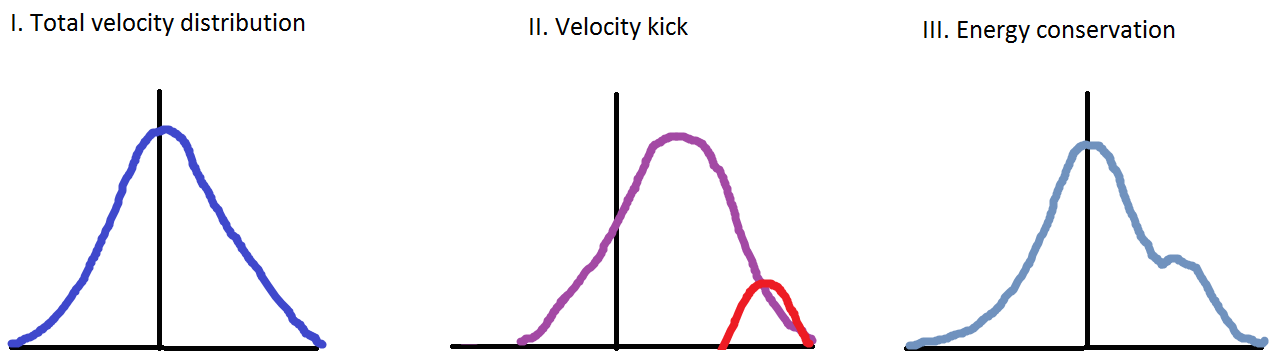
\includegraphics[width=15.0 cm]{img/Energy_exchange.png}
\caption{This simple cartoon illustrate the effects of the energy exchange simulation on the total velocity distribution. I: The initial distribution of the total velocity given in terms of cartesian coordinates,
$v=\sqrt{v_x^2+v_y^2+v_z^2}$. It follows a Gaussian shape with mean velocity equal to zero. \\
II: Velocity kicks are now given to each particle in the structure, by multiplication of the initial velocities with a uniformly distributed random number in the range [0.8, 1.2]. This has the effect of shifting the mean of the distribution towards higher values. Furthermore, some of the particles with very high velocities (and further away from the structures center, where the potential is weaker) now become gravitationally unbound. This is illustrated by the red bump at the right tail of the right-shifted, randomized velocity curve shown in purple. The total energy is now higher than what it was initially. As the velocities were perturbed by factors in the range [0.8, 1.2], the kinetic energies $K \propto v^2$ will have their initial values changed by factors in the range [0.64, 1.44] giving a new kinetic energy span of [1-0.36, 1+1.44] times the initial kinetic energies.\\
III: In order to conserve energy, a normalization factor is multiplied with the initial energy, and used to normalize particle velocities after the previous randomization, so that the velocity mean of zero is regained. A small bump at the right tail remains however, which is seen on the final curve shown in pale blue.}
\label{fig:test}
\end{figure}

\begin{table}[!htbp]
\centering
\begin{tabular}{|c|c|c|}
 \hline
 Run No. & velocity kicks &  Flow time  \\ \hline
   0     &     0 $\%$     &     100     \\ \hline
 1-10    &    20 $\%$     &     100     \\ \hline
 11-20	 &     5 $\%$     &     100     \\ \hline
 21-30	 &    30 $\%$     &     100     \\ \hline
 31-40	 &    30 $\%$     &     500     \\ \hline
\end{tabular}
\caption {Simulation II pattern. The left column shows the number of run in question. 
The middle column gives the maximum percentage of velocity kick to each particle along each of the three cartesian velocity directions, $v_x$, $v_y$ and $v_z$. Finally the right column states the time allowed for structures to flow freely under their self gravity. Run 0 takes place without any prior perturbation and lasts for 100 simulation times. In short, all structures are given medium velocity kicks before the first 10 runs following perturbations (run 1 $\rightarrow$ 10), while they are given small kicks before run 11 $\rightarrow$ 20, large kicks are given for run 21 $\rightarrow$ 40. Each of the runs from 1 $\rightarrow$ 30 lasts for 100 simulation times, but the last 10 runs (31 $\rightarrow$ 40) are given 500 simulation times each.}
\end{table}

This whole process of velocity-kick and energy normalization is followed by a phase of flow after which the pattern is repeated (kick $\rightarrow$ flow). A parallel control simulation (with 20 runs) is performed where the energy is not exchanged in this manner. No alterations are done; i.e. G remains at unity throughout and no velocity kicks are given by hand to any particle. The purpose of this control simulation is to make sure the structures stay in equilibrium and provide a means of comparison for the perturbed structures. 
Binning of structures is done in the following way:
First the radius of all particles to the halo center is sorted from smallest to largest value and this sorting is then applied to the positions and velocities as well as the potential. Now number bins are created so that each bin holds exactly 500 particles and runs from smallest to largest radii. The volume of each bin is hence generally different and depends on the mean inter-particle distance which grows as radius increases. It is therefore the case that outermost bins take up more space than innermost number-bins. Inside each number bin the perturbation and normalizing of particle velocities and energies can then be performed. Finally saving the perturbed structures into a new snapshotfile, this is then ready to be read and simulated by the GADGET-2 code. More specifically about the perturbations:
Starting out by giving each particle a velocity kick by a random number in the above stated range for each of its three cartesian velocity directions provide the particles with a new velocity given by 

\centerline{$v_{rand} = \sqrt{v_{x,rand}^2 + v_{y,rand}^2 + v_{z,rand}^2}$}

where for example 

\centerline{$v_{z,rand} = v_z^{initial} + \Delta v_z = v_z^{initial}\big( 1 + rand[0.8,1.2] \big) $}

and 	$rand[0.8,1.2]$ is a uniform random number between 0.8 and 1.2, thus perturbing each of the cartesian velocity components by maximally 20 \% which in turn means that the maximum perturbation to the total velocity vector can be $\sqrt{1200} \% = 20\cdot \sqrt{3} \% \approx 34.6 \%$.
The kinetic energy becomes 

\centerline{$K_{rand}=\frac{1}{2}v_{rand}^2$}

In order to ensure energy conservation normalization factors must be multiplied to the new velocities.
The particles are split into gravitationally bound (where $\Phi + K \leq 0 $) and unbound (where $\Phi + K > 0 $). The unbound particles new velocities are first multiplied by a random number in the range $[0.8, 1.0]$ and subsequently normalized by multiplying them with 

\centerline{$ \sqrt{\frac{ \sum |\Phi|}{ \sum K_{rand}}}$} 

After this normalization the kinetic energy is determined as 

\centerline{$K_{rand, norm}=\frac{1}{2}v_{new}^2$,} 

where $v_{new}$ is the concatenation of initially bound, and the now bound particles (after normalization).
Then the new cartesian velocities are normalized by multiplying them with 

\centerline{$ \sqrt{\frac{<K_{initial}>}{<K_{rand, norm}>}}$,} 

where $<K_{initial}>$ and $<K_{rand, norm}>$ are the kinetic energies initially and after randomization plus normalizations, respectively. This gives the final velocities 

\centerline{$v_{final} = \sqrt{v_{x,final}^2 + v_{y,final}^2 + v_{z,final}^2}$}

Now the kinetic energy is $K_{final}=\frac{1}{2}v_{final}^2$ and the average value equals the average of the initial kinetic energy.

\begin{figure}[!htbp]
\centering
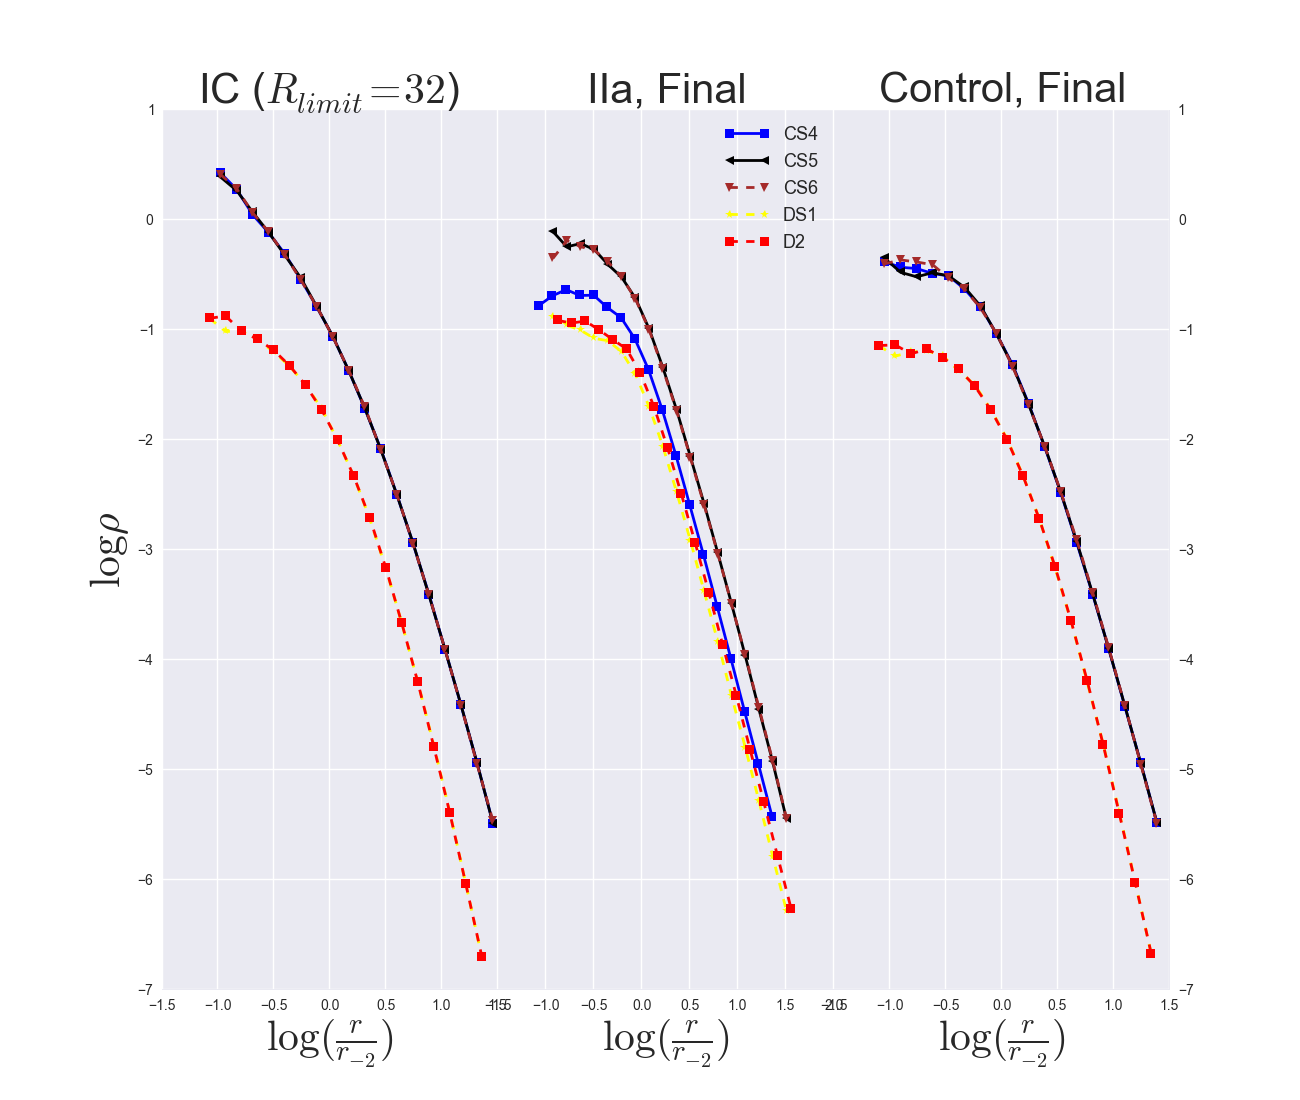
\includegraphics[width=1.0\linewidth]{img/logr_logrho.png}
\caption{Density profiles. $\log (\rho)$ vs. $\log \frac{r}{r_{-2}}$ for Sim. IIa of stable structures $CS_4$, $CS_5$, $CS_6$, $DS_1$ and $D_2$. First subplot from the left shows the IC's, middle subplot shows final products and right subplot shows final products of the control runs where no perturbations were applied to any of the structures. The right subplot thus serves as a efficient means of comparison with the final products of Sim. IIa. The formation of a core is seen for the final products as time evolves. 20 radial bins is used for these structures which have $N = 10^5$ particles.}
\label{fig:test}
\end{figure}

\begin{figure}[!htbp]
\centering
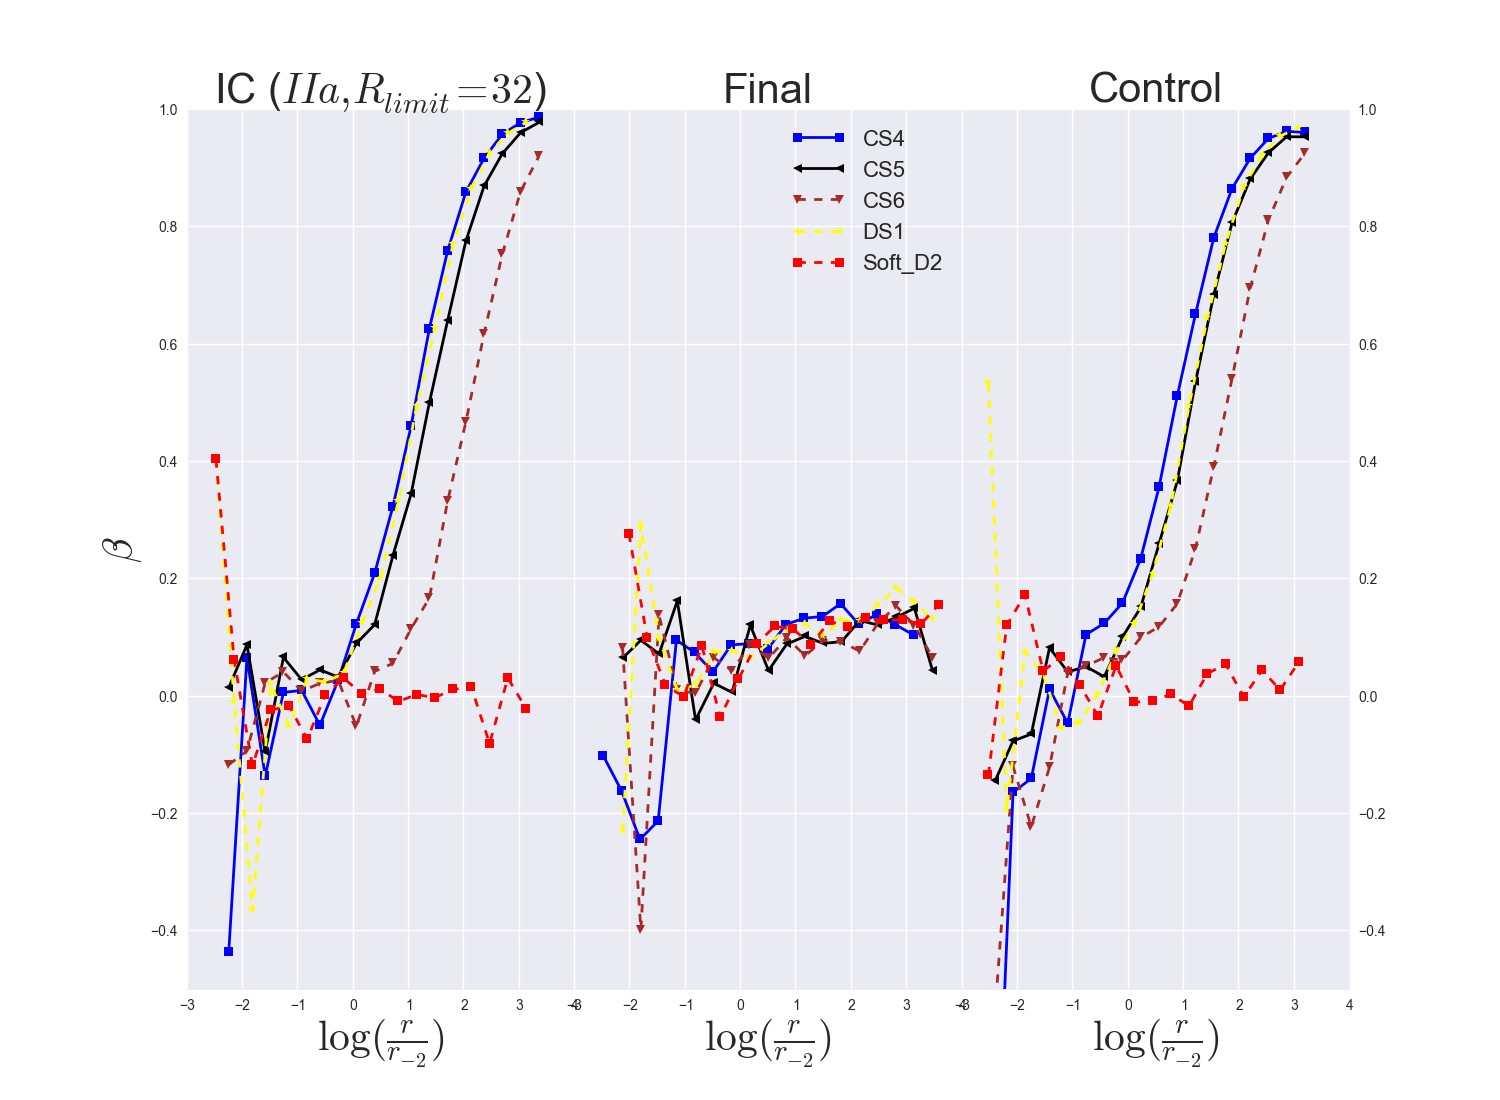
\includegraphics[width=1.0 cm]{img/log_r_r2_beta_CS4CS5CS6DS1D2_Rlimit32.png}
\caption{$\beta$ profiles for Sim. IIa of stable structures $CS_4$, $CS_5$, $CS_6$, $DS_1$ and $D_2$.
Structures are cut off at a radius of 32 times the scale radius. 20 radial bins are used. 
Initial conditions with either complete velocity isotropy or slightly anisotropic ones are both seen to be driven towards a new attractor
in the outer regions where they tend to land close to $\beta = 0.1$ (see middle panel).
The control runs which are simulated with no perturbations interfering can be seen in the right panel.
They show no significant departure from the initial conditions shown in the left panel.}
\label{fig:test}
\end{figure}

\begin{figure}[!htbp]
\centering
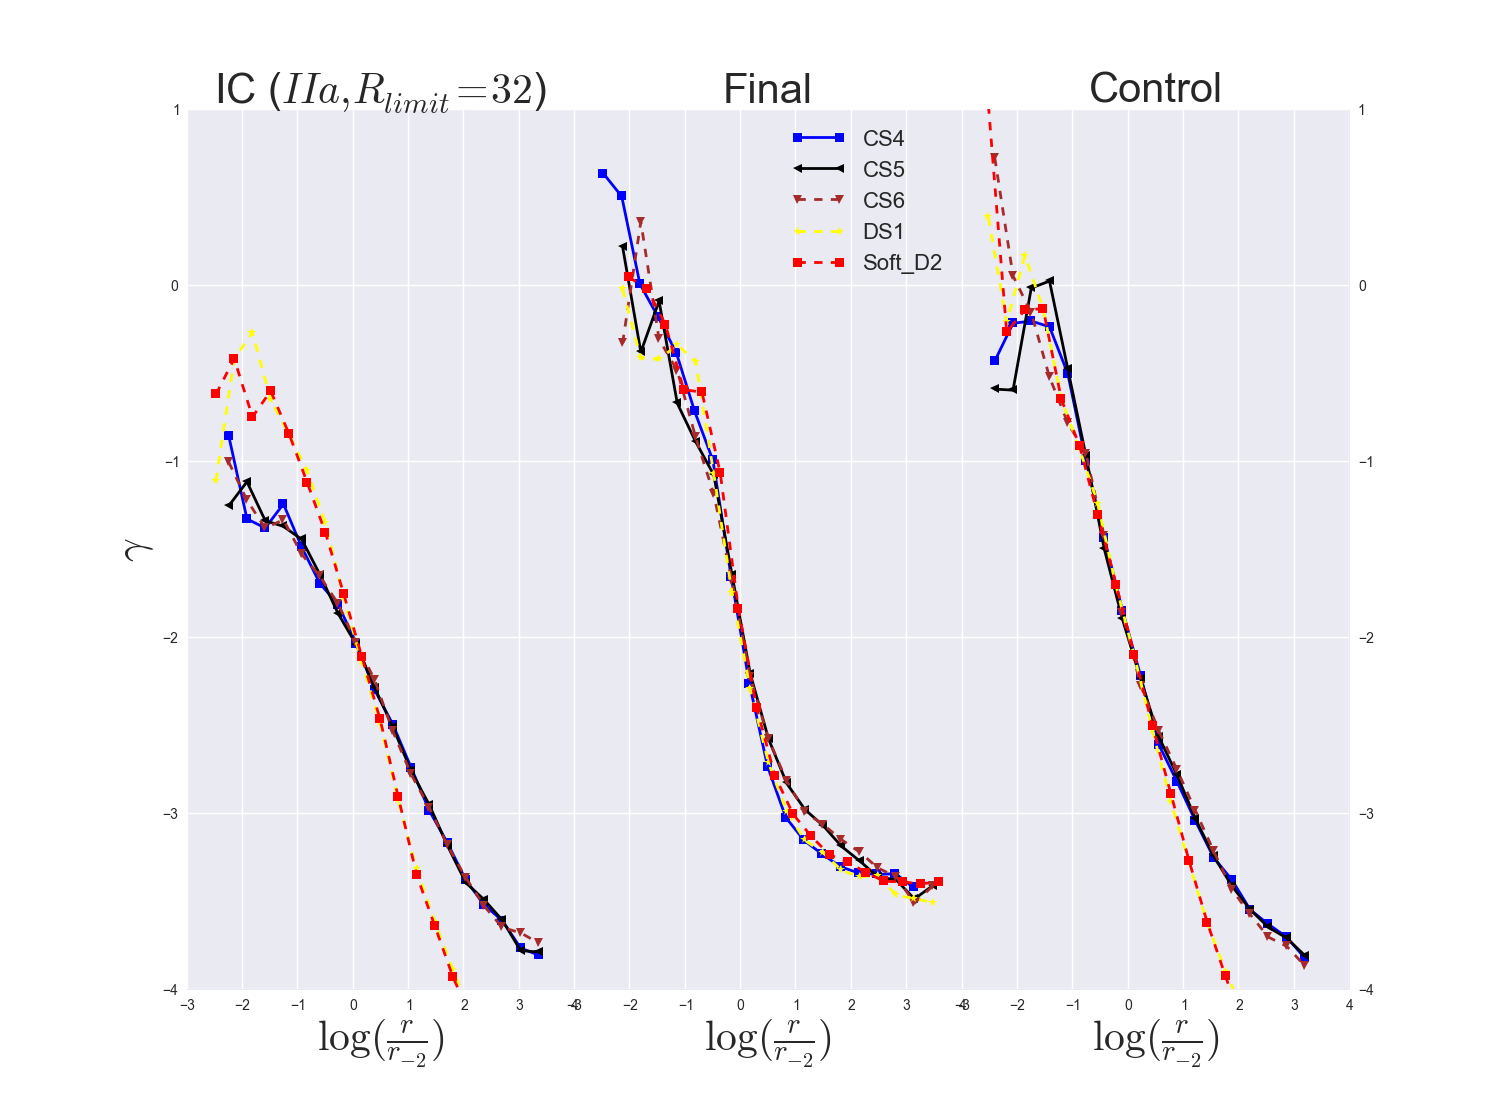
\includegraphics[width=1.0 cm]{img/log_r_r2_gamma_CS4CS5CS6DS1D2_Rlimit32.png}
\caption{$\gamma$ profiles for Sim. IIa of stable structures $CS_4$, $CS_5$, $CS_6$, $DS_1$ and $D_2$.
Structures are cut off at a radius of 32 times the scale radius. 20 radial bins are used. 
The final structures in the middle panel can be seen to get attracted towards a characteristic curve.
The $\gamma$ profiles thus have a preferred structure as very different initial conditions all flow towards this configuration.
The control runs which are simulated with no perturbations interfering can be seen in the right panel.
They show no significant departure from the initial conditions shown in the left panel.}
\label{fig:test}
\end{figure}

\begin{figure}[!htbp]
\centering
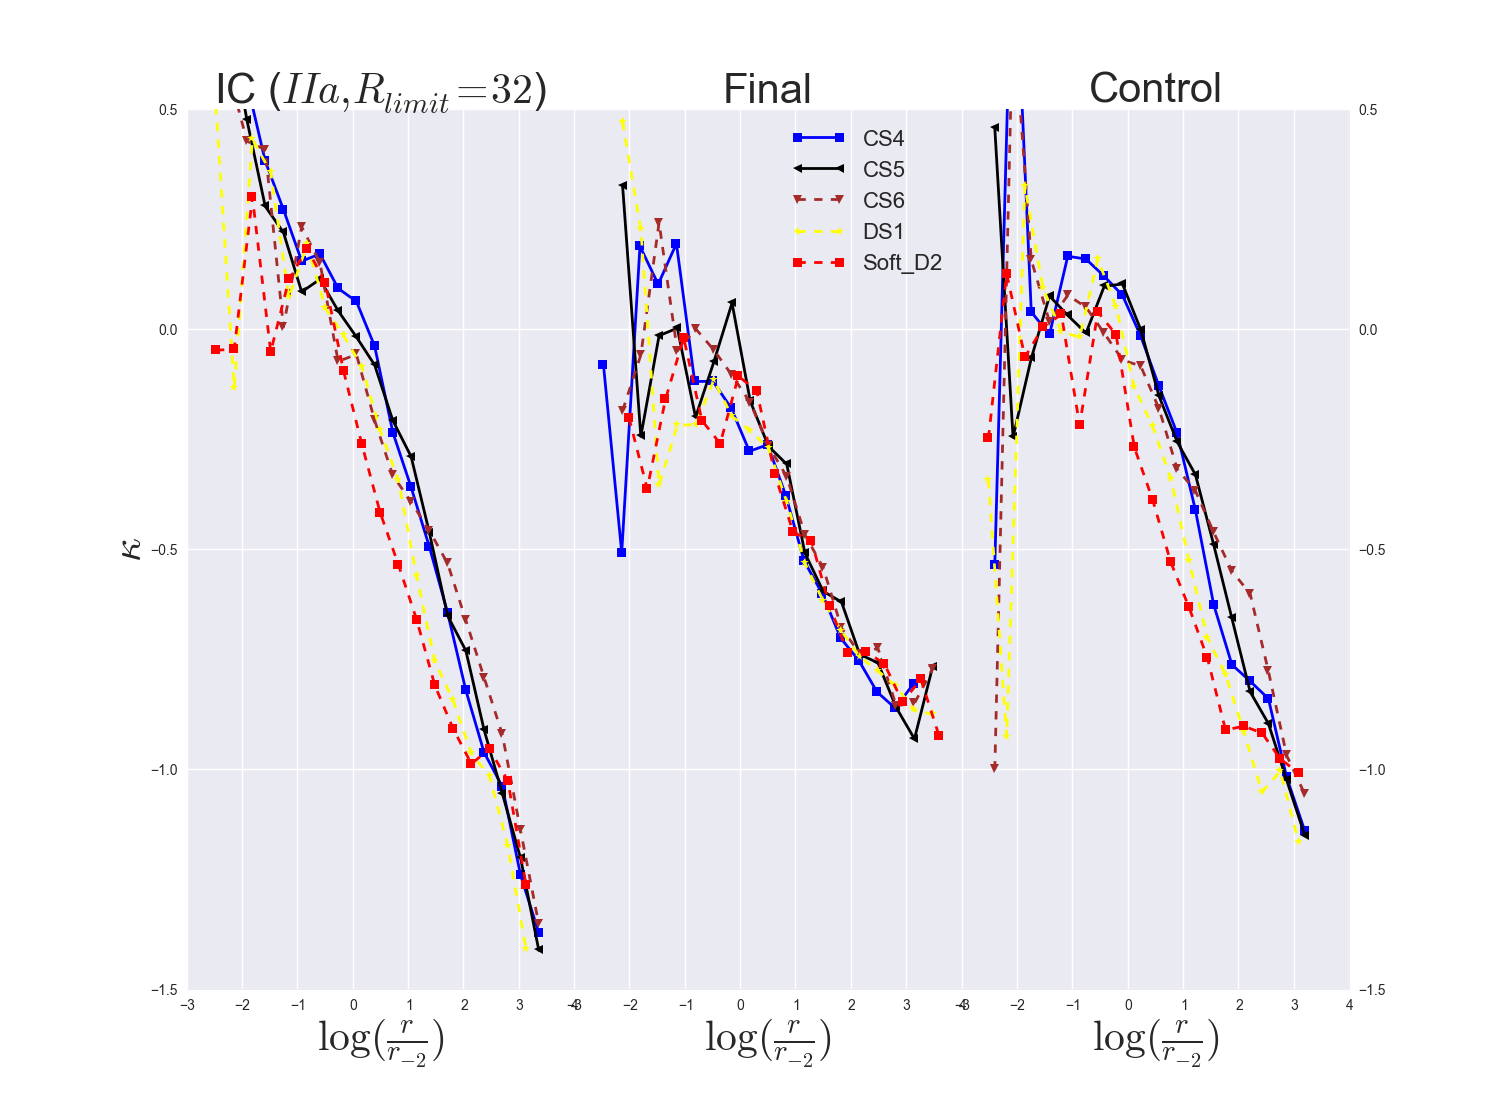
\includegraphics[width=1.0 cm]{img/log_r_r2_kappa_CS4CS5CS6DS1D2_Rlimit32.png}
\caption{$\kappa$ profiles for Sim. IIa of stable structures $CS_4$, $CS_5$, $CS_6$, $DS_1$ and $D_2$.
Structures are cut off at a radius of 32 times the scale radius. 20 radial bins are used. 
The middle panel reveals an attractor for the end products wrt. the $\kappa$-profiles.
This attractor is present for $\log \frac{r}{r_{-2}} > 0.5$. 
The control runs which are simulated with no perturbations interfering can be seen in the right panel.
They show no significant departure from the initial conditions shown in the left panel.}
\label{fig:test}
\end{figure}

\begin{figure}[!htbp]
\centering
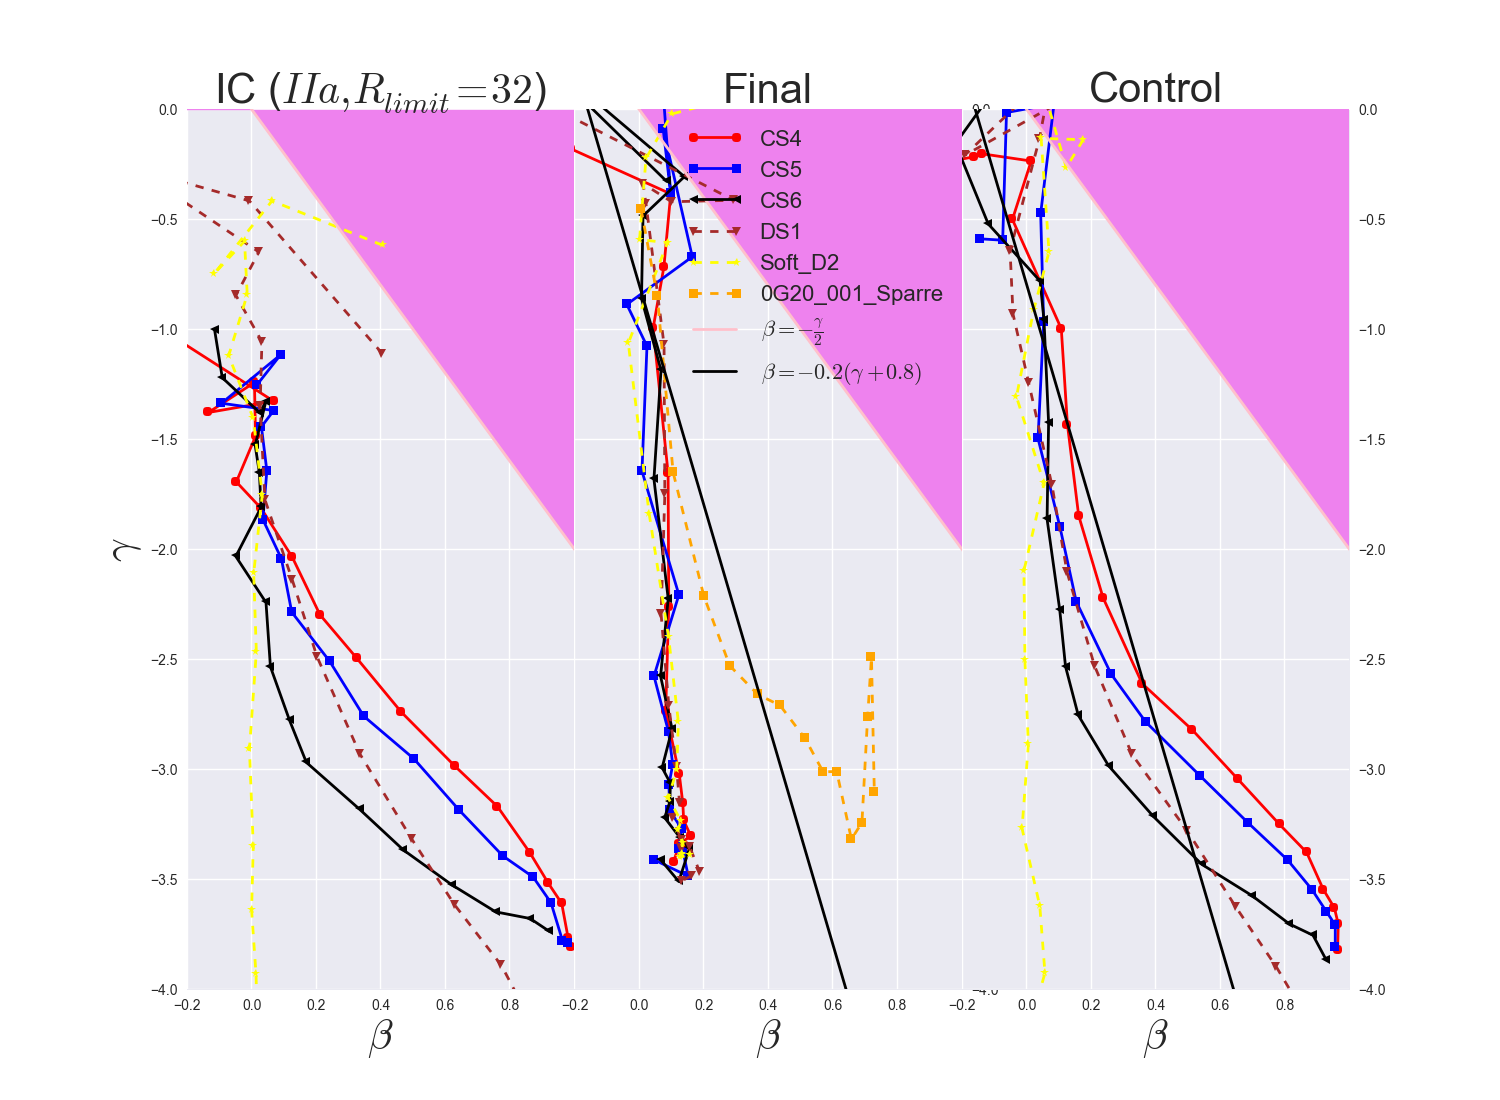
\includegraphics[width=1.0 cm]{img/beta_vs_gamma_CS4CS5CS6DS1D2_Rlimit32.png}
\caption{Attractor plot in the ($\beta$,$\gamma$)-space for Sim. IIa of stable structures $CS_4$, $CS_5$, $CS_6$, $DS_1$ and $D_2$. Structures are cut off at a radius of 32 times the scale radius. 20 radial bins are used. The left panel shows how the initial conditions spread out and fill up a large volume in the stable region of the Jeans parameter space spanned by $\beta$ and $\gamma$. This makes the attractor very apparent in the middle panel where structures are driven towards $\beta = 0.1$ in the outer regions. Final products are shown together with a final product from a sim. of type I performed by S.H. Hansen and M. Sparre for comparison. Also shown is the linear $\beta$-$\gamma$ relation discovered by Hansen and Moore (2006) for comparison. The pink upper right area is found to be an unstable region by An and Evans (2006).The control runs which are simulated with no perturbations interfering can be seen in the right panel. They show no significant departure from the initial conditions shown in the left panel.}
\label{fig:test}
\end{figure}

\begin{figure}[!htbp]
\centering
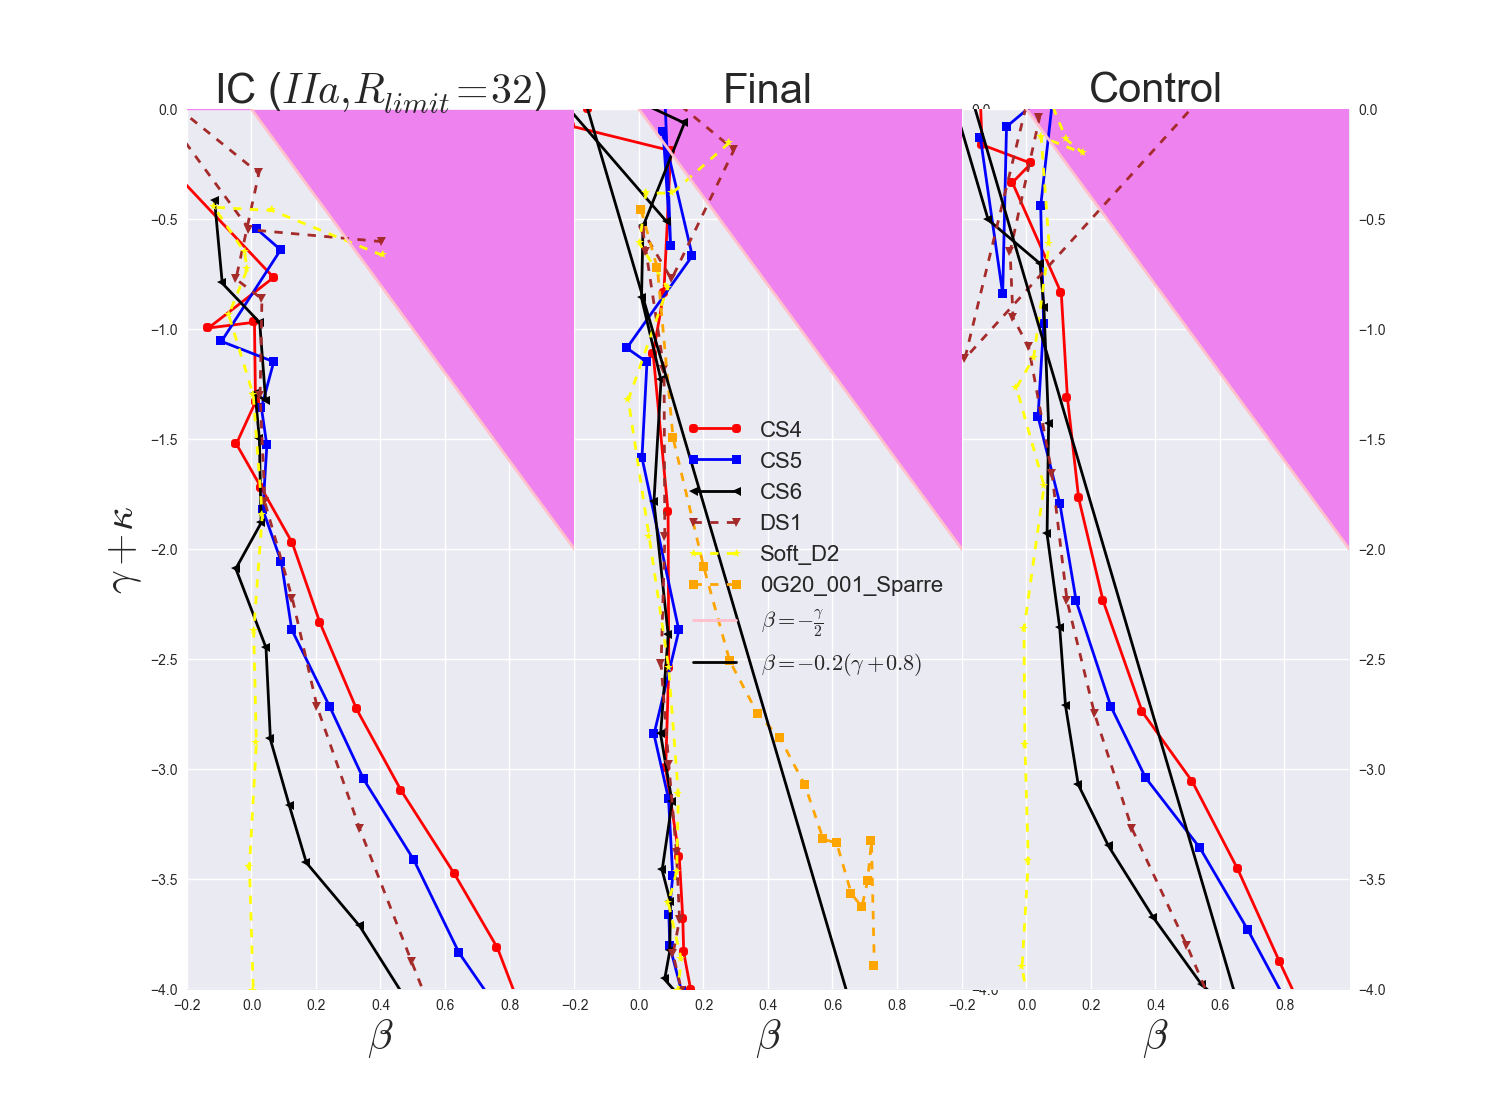
\includegraphics[width=1.0 cm]{img/beta_vs_gamma_plus_kappa_CS4CS5CS6DS1D2_Rlimit32.png}
\caption{Attractor plot in the ($\beta$,$\gamma + \kappa$)-space for Sim. IIa of stable structures $CS_4$, $CS_5$, $CS_6$, $DS_1$ and $D_2$.
Structures are cut off at a radius of 32 times the scale radius. 20 radial bins are used. In this projection the attractor is still clearly seen. We still compare it with the results found by others. The control runs which are simulated with no perturbations interfering can be seen in the right panel. They show no significant departure from the initial conditions shown in the left panel.}
\label{fig:test}
\end{figure}

\subsubsection{IIb: Energy exchange (radial velocity perturbations)}
\textbf{Using structures $CS_4$ and $D_2$, this simulation perturbs only the radial velocities of particles. Specifically, for all of these structures the total velocities inside spherical bins is perturbed for each of its particles by multiplying those given particles radial velocities ($v_r$) by random numbers in the range $[0.7, 1.3]$ (corresponding to perturbing the kinetic energies by random numbers in the range $\frac{1}{2}\cdot[0.49, 1.69]$), taken from the continuous uniform distribution. Following this exchange of kinetic energies between particles in fixed spherical bins, a normalization factor is applied to the total velocities, which ensures energy conservation. it has the same functional form as the one applied in sim. IIa, but will yield different numerical values as sim. $II_b$ does not perturb all three spherical velocities but only the radial one. The normalization factor will thus be smaller in this sim. After these velocity kicks the structures are simulated under their self gravity allowing them to flow a bit under their new velocities. This procedure is then repeated for a total of 20 runs (with one initial run where there is no perturbation. This allows the OM models to reach equilibrium, as they are not perfectly equilibrated when set up as OM models. It is done for Edd structures as well to be certain of equilibrium before any perturbations take effect). After the first 10 runs, the random number range is unchanged but the runs 11 $\rightarrow$ 20 are given longer timespans ($t_{sim} = 500$ corresponding to 5 dynamical times at $r = 12.7r_s$) to allow structures more flow.} \\ \\

Starting from the Cartesian quantities (coordinates and velocities) one of the first steps in the algorithm used for the perturbations is to perform a transformation into spherical quantities. This can be done by applying a function F which maps real values from the cartesian domain $R^3$ onto the spherical range $R^+ \times [0,\pi] \times [0,2\pi)$. F has the components: \\ 

\begin{align*}
R          & = \sqrt{x^2+y^2+z^2} \\
\theta     & = arccos(\frac{z}{R}) \\
\phi       & = arctan(\frac{y}{x}) \\
v_R        & = sin(\theta)cos(\phi)v_x+sin(\theta)sin(\phi)v_y+cos(\theta)v_z \\
v_{\theta} & = cos(\theta)cos(\phi)v_x+cos(\theta)sin(\phi)v_y-sin(\theta)v_z \\
v_{\phi}   & = - sin(\phi)v_x + cos(\phi)v_y \\
\end{align*}

The coordinate transformation from Cartesian to spherical curvilinear coordinates has the following Jacobian matrix:

\begingroup
\renewcommand*{\arraystretch}{2.5}
\begin{equation}
J_F(x,y,z) = 
\begin{bmatrix}
\dfrac{\partial R}{\partial x} & \dfrac{\partial R}{\partial y} & \dfrac{\partial R}{\partial z} \\ 
\dfrac{\partial \theta}{\partial x} & \dfrac{\partial \theta}{\partial y} & \dfrac{\partial \theta}{\partial z} \\ 
\dfrac{\partial \phi}{\partial x} & \dfrac{\partial \phi}{\partial y} & \dfrac{\partial \phi}{\partial z} 
\end{bmatrix} =
\begin{bmatrix}
\dfrac{x}{R} & \dfrac{y}{R} & \dfrac{z}{R} \\ 
0            &   0          & -\dfrac{1}{\sqrt{R^2-z^2}} \\ 
-\dfrac{y}{x^2+y^2} &  \dfrac{x}{x^2+y^2} & 0 
\end{bmatrix}
\end{equation}
\endgroup

The determinant of this Jacobian matrix is $\frac{1}{\sqrt{R^2-z^2}}$

Now the spherical velocities are ready to be manipulated inside the number bins.
Radial velocities are randomized as described above, and the speed is found as
$ v_{tot} = \sqrt{v_R^2 + R^2v_{\theta}^2 + R^2v_{\phi}^2sin(\theta)^2}$.
Some of the particles might become gravitationally unbound after this procedure. This is checked and any such unbound particles are rebound by multiplying their new randomized radial velocity component by another random number in the range [0.8,1.0] and then a normalization factor of $\sqrt[|\Phi|]{K_{rand}}$, where $|\Phi|$ is the numerical value of the gravitational potential inside any particular bin and $K_{rand}$ is the total kinetic energy of the unbound particles inside that bin.
A final normalization factor is then applied to all particles inside any given bin in order to obtain energy conservation. This factor is given by $K_{ratio} = \sqrt[<K_{init}>]{<K_{final}>}$, where $<K_{init}>$ is the initial total kinetic energy of the particles inside that bin and $<K_{final}>$ is the final total kinetic energy of the particles inside that bin. The operation to ensure energy conservation thus becomes: $ v_{R,final} = v_{R,init} \cdot K_{ratio} $, where $v_{R,init}$ are the velocities prior to the perturbation.  

Final step of the perturbation algorithm is to transform spherical quantities back to Cartesian (so that the perturbed structure can be saved as a snapshot-file of correct format which the GADGET-2 code can then read and simulate). This can be done by applying another function F, which maps the spherical domain $R^+ \times [0,\pi] \times [0,2\pi)$ onto the Cartesian range $R^3$. This new F giving the back-transformation has the components: \\ 

\begin{align*}
x   &= Rsin(\theta)cos(\phi) \\
y   &= Rsin(\phi)sin(\theta) \\
z   &= Rcos(\theta) \\
v_x &= sin(\theta)cos(\phi)v_R + cos(\phi)cos(\theta)v_{\theta} - sin(\phi)v_{\phi} \\
v_y &= sin(\phi)sin(\theta)v_R + sin(\phi)cos(\theta)v_{\theta} + cos(\phi)v_{\phi} \\
v_z &= cos(\theta)v_R - sin(\theta)v_{\theta}
\end{align*}

The coordinate transformation from spherical to Cartesian coordinates has the following Jacobian matrix:

\begingroup
\renewcommand*{\arraystretch}{2.5}
\begin{equation}
J_F(r,\theta,\phi) = 
\begin{bmatrix}
\dfrac{\partial x}{\partial R} & \dfrac{\partial x}{\partial \theta} & \dfrac{\partial x}{\partial \phi} \\ 
\dfrac{\partial y}{\partial R} & \dfrac{\partial y}{\partial \theta} & \dfrac{\partial y}{\partial \phi} \\ 
\dfrac{\partial z}{\partial R} & \dfrac{\partial z}{\partial \theta} & \dfrac{\partial z}{\partial \phi} 
\end{bmatrix} =
\begin{bmatrix}
sin(\theta)cos(\phi) &  Rcos(\theta)cos(\phi)  & -Rsin(\theta)sin(\phi)  \\ 
sin(\theta)sin(\phi) &  Rcos(\theta)sin(\phi)  &  Rsin(\theta)cos(\phi)  \\ 
cos(\theta)          & -Rsin(\theta)  &  0 
\end{bmatrix}
\end{equation}
\endgroup

The determinant of this Jacobian matrix is $R^2sin(\theta)$.

\begin{figure}[!htbp]
\centering
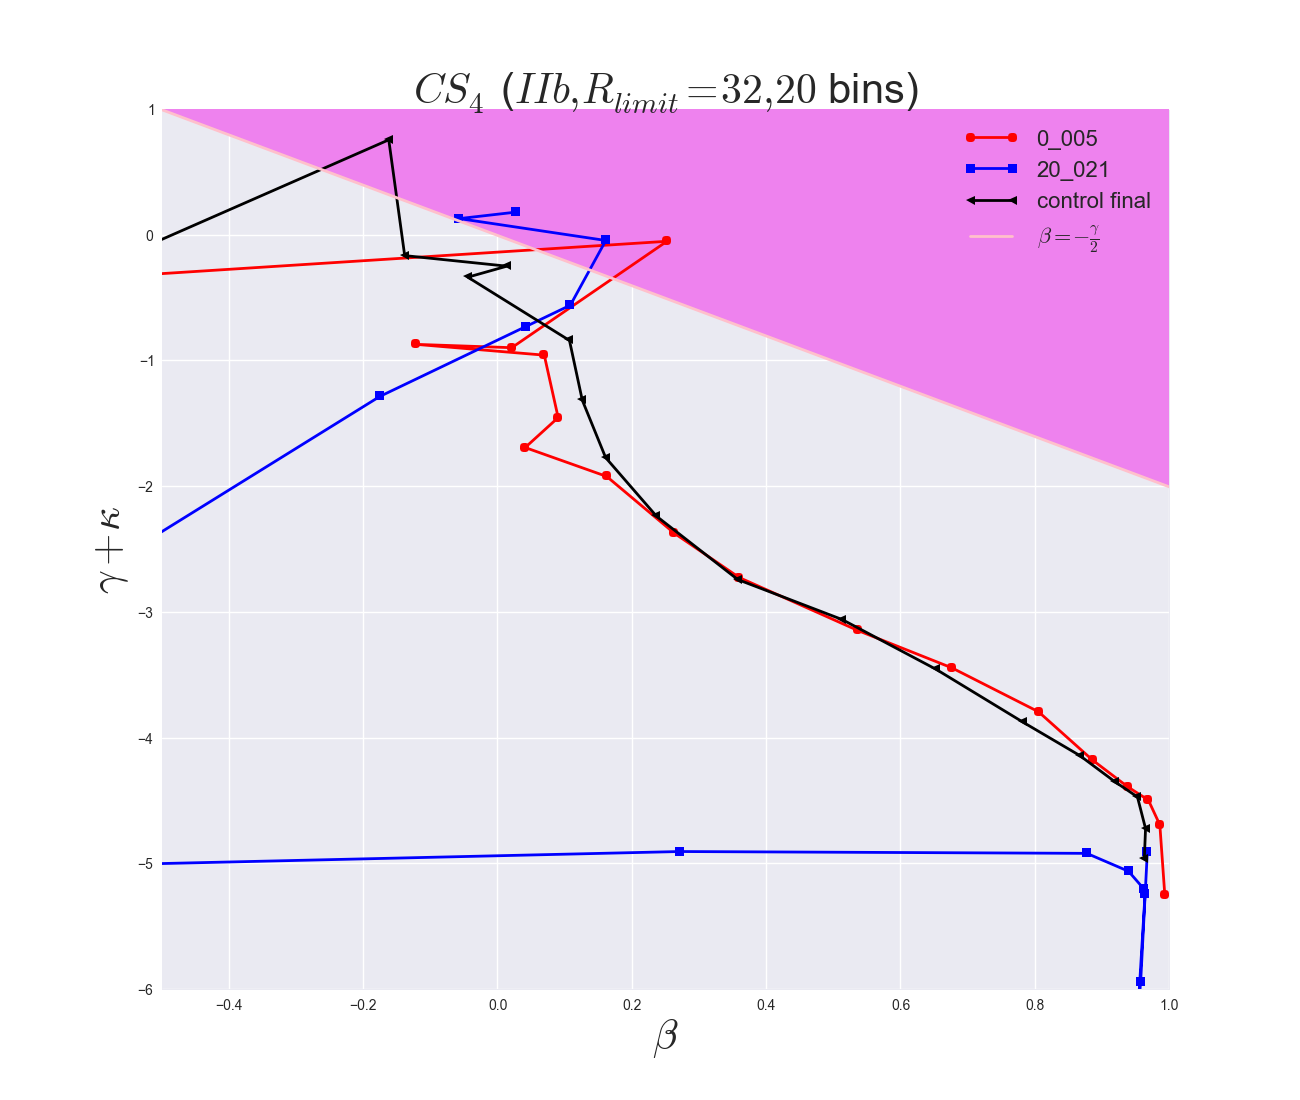
\includegraphics[width=1.0\linewidth]{img/beta_vs_gamma_plus_kappa_IIb_CS4_Rlimit32.png}
\caption{$\gamma + \kappa$ vs. $\beta$ for IC, final product and control run of sim. IIb, of stable structure $CS_4$.
Structures are cut off at a radius of 32 times the scale radius. 20 radial bins are used.
No attractor is found. This agrees with work done by others [4]. The conclusion here must be then that not all perturbations will work when trying to reveal natures attractors. In [4] this is compared to a ball being continuously kicked uphill. The ball might wish to fall down (flow) but never get a chance to if it is repeatedly being kicked upwards (e.g. radially perturbed as in this case). Perhaps this experiment is just not in agreement with any physical process.}
\label{fig:test}
\end{figure}

\begin{figure}[!htbp]
\centering
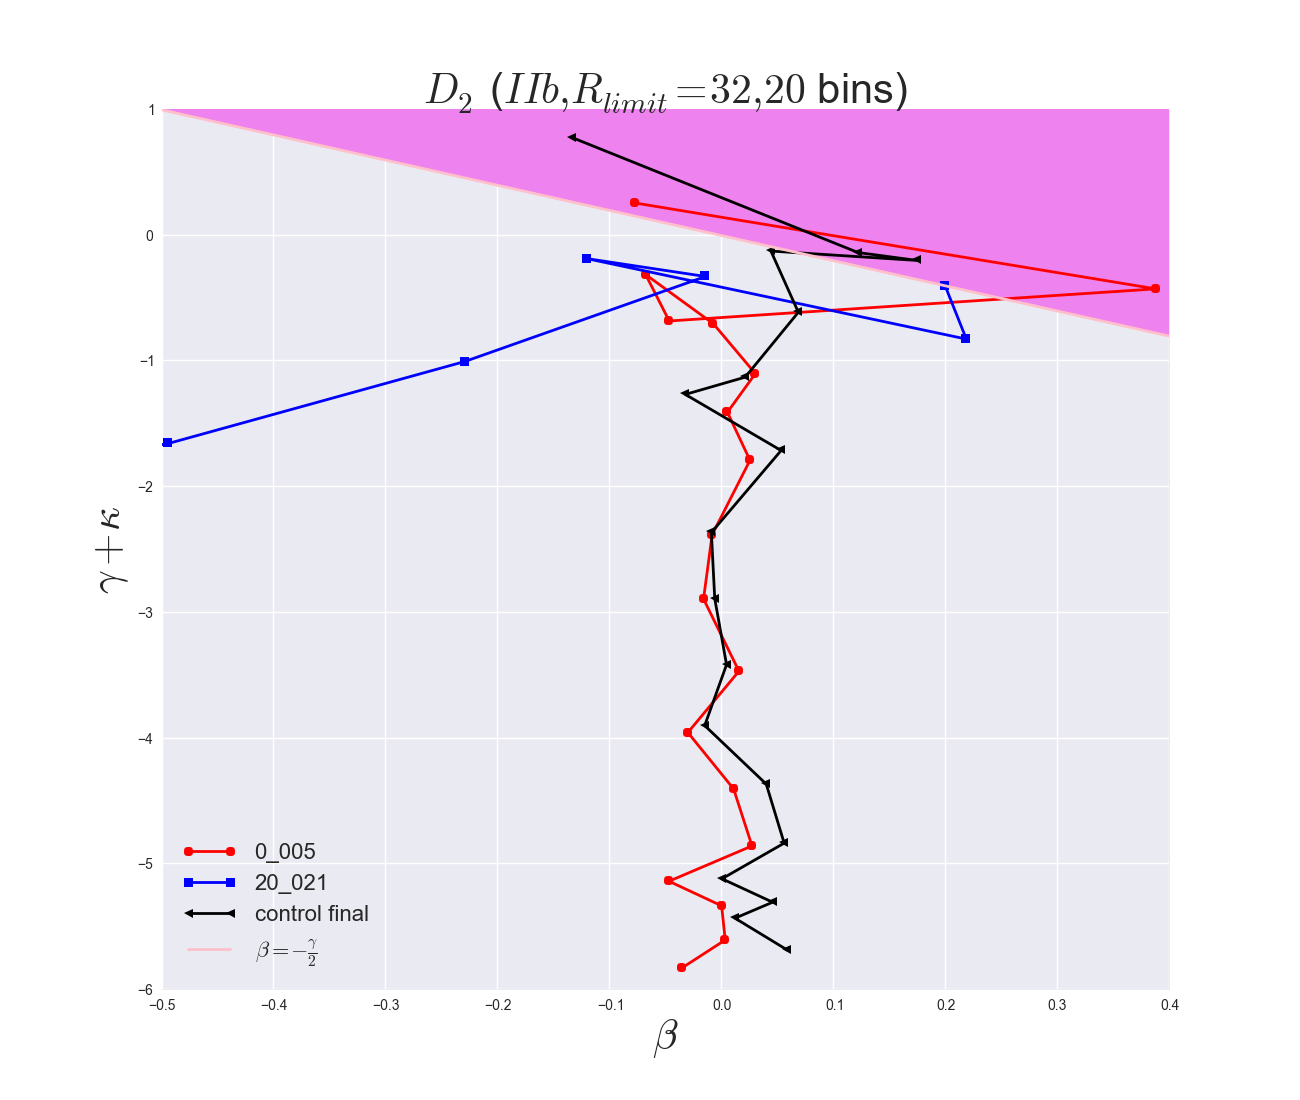
\includegraphics[width=1.0\linewidth]{img/beta_vs_gamma_plus_kappa_IIb_D2_Rlimit32.png}
\caption{$\gamma + \kappa$ vs. $\beta$ for IC and final product of sim. $II_b$ of structure $D_2$.
Structures are cut off at a radius of 32 times the scale radius. 20 radial bins are used.
No attractor is found. This agrees with work done by others [4]. The conclusion here must be then that not all perturbations will work when trying to reveal natures attractors. In [4] this is compared to a ball being continuously kicked uphill. The ball might wish to fall down (flow) but never get a chance to if it is repeatedly being kicked upwards (e.g. radially perturbed as in this case). Perhaps this experiment is just not in agreement with any physical process.}
\label{fig:test}
\end{figure}

\subsubsection{IIc: Energy exchange (tangential velocity perturbations)}
\textbf{Using structures $CS_4$ and $D_2$, this simulation perturbs only the tangential velocities of particles. Specifically, for all of these structures the total velocity inside spherical bins is perturbed for each of its particles by multiplying those given particles tangential velocities $v_{\theta}$ and $v_{\phi}$ by random numbers in the range $[0.9, 1.1]$ before each of the first ten simulations (each lasting for a duration of 1 $t_{dyn}$ at $r = 12.7 r_s$) and 
random numbers in the range $[0.7, 1.3]$ before each of the next twenty (for $D_2$) or ten (for $CS_4$) simulations (each of which this time lasting for a duration of 5 $t_{dyn}$ at $r = 12.7 r_s$, allowing structures more flow) (corresponding to perturbing the kinetic energies by random numbers in the range $\frac{1}{2}\cdot[0.49, 1.69]$), taken from the continuous uniform distribution. Following this exchange of kinetic energies between particles in fixed spherical bins, a normalization factor is applied to the total velocities, which ensures energy conservation. it has the same functional form as the one applied in sim. $II_a$, but will yield different numerical values as sim. IIc does not perturb all three spherical velocities but only the two tangential ones. The normalization factor will thus be smaller in IIc than the one utilized in IIa but on average larger than the one in $II_b$. After these velocity kicks the structures are simulated under their self gravity allowing them to flow a bit under their new velocities. This procedure is then repeated for a total of 20 runs for $CS_4$ and 30 runs for $D_2$ (with one initial run where there is no perturbation. This allows the OM models to reach equilibrium, as they are not perfectly equilibrated when set up as OM models. It is done for Edd structures as well to be certain of equilibrium before any perturbations take effect). $CS_4$ only gets 20 runs as it does not change significantly and thus already seem to start out at a stable point. $D_2$ is however simulated for 30 runs at it changes significantly after each simulation. After 20 runs it has reached a stable point where the next 10 runs until run 30 has no real effect on $D_2$ at all.} \\ \\

Similarly to $II_b$, the $II_c$ sim. transforms Cartesian into spherical quantities, divides the structure into particle number bins, perturbs and normalize velocities and energy, and finally transforms back to Cartesian form followed by saving into a new snapshotfile which can then be read and simulated by the GADGET-2 code.

\begin{figure}[!htbp]
\centering
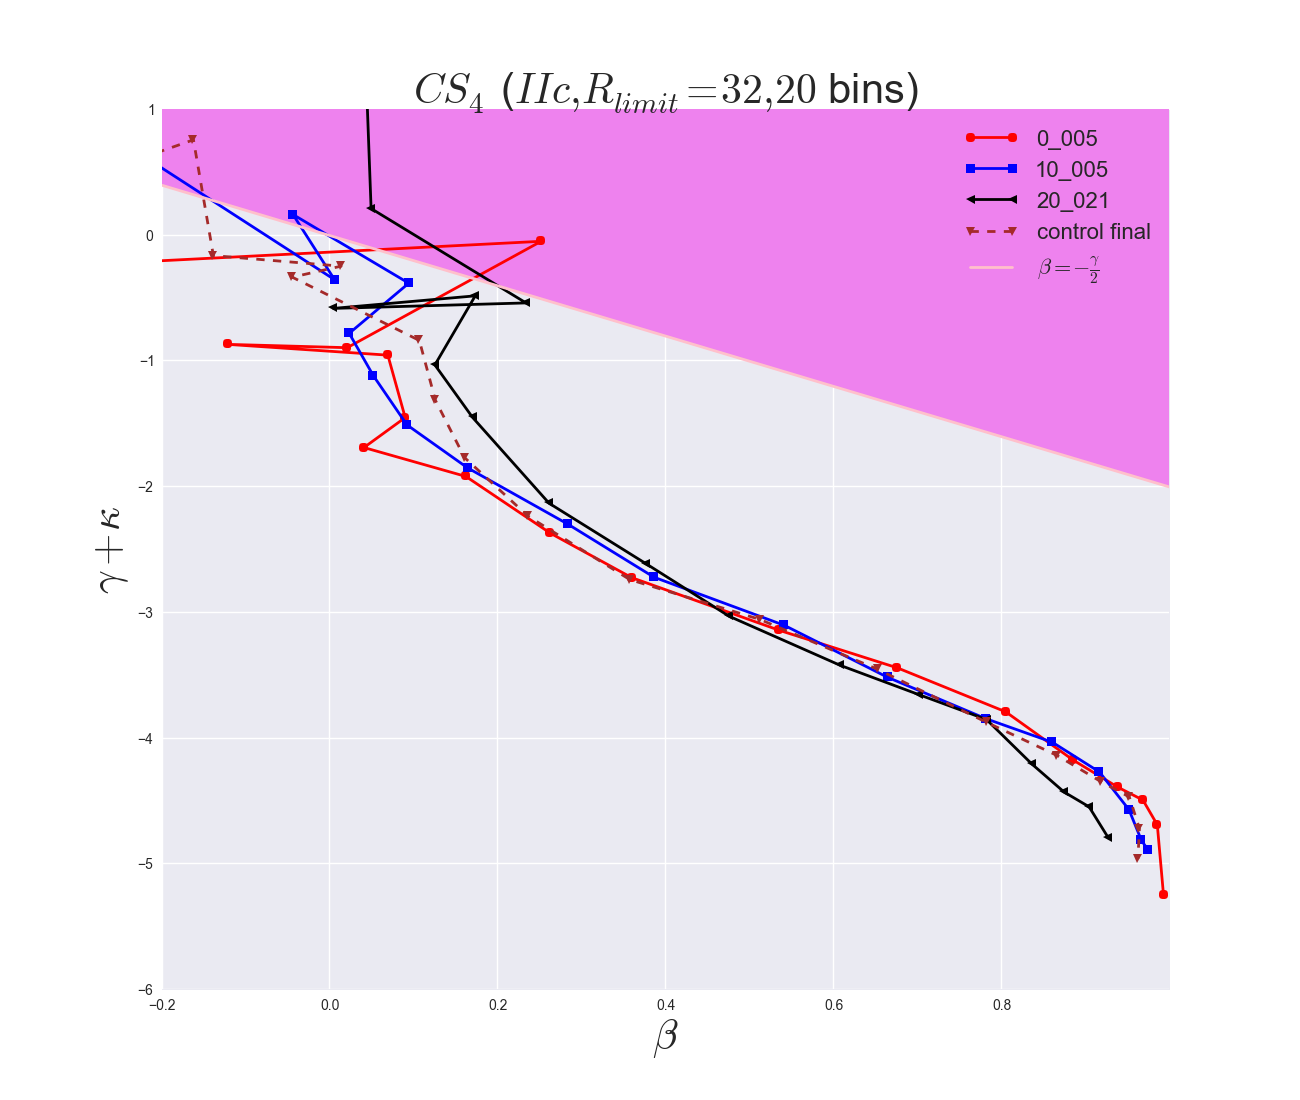
\includegraphics[width=1.0\linewidth]{img/beta_vs_gamma_plus_kappa_IIc_CS4_Rlimit32.png}
\caption{$\gamma + \kappa$ vs. $\beta$ for IC, 10, final product and control run of sim. IIc of structure $CS_4$. Structures are cut off at a radius of 32 times the scale radius. 20 radial bins are used.
No change is seen at any part of this structure from $\beta = 0.2$ and upwards. The inner fluctuations where $\beta$ is smaller can be attributed to numerical noise as the radii here moves close to the softening length of the sim. The lack of change is most probably that structure $CS_4$ already starts out very close to the attractor and therefore remains here. When analyzing the shape of this structure up close it is seen to fulfill the attractor values already found in [4], namely $(\gamma + \kappa) = -8\beta$ for smaller radii and $(\gamma + \kappa) = -0.7-4\beta$ for larger radii.}
\label{fig:test}
\end{figure}

\begin{figure}[!htbp]
\centering
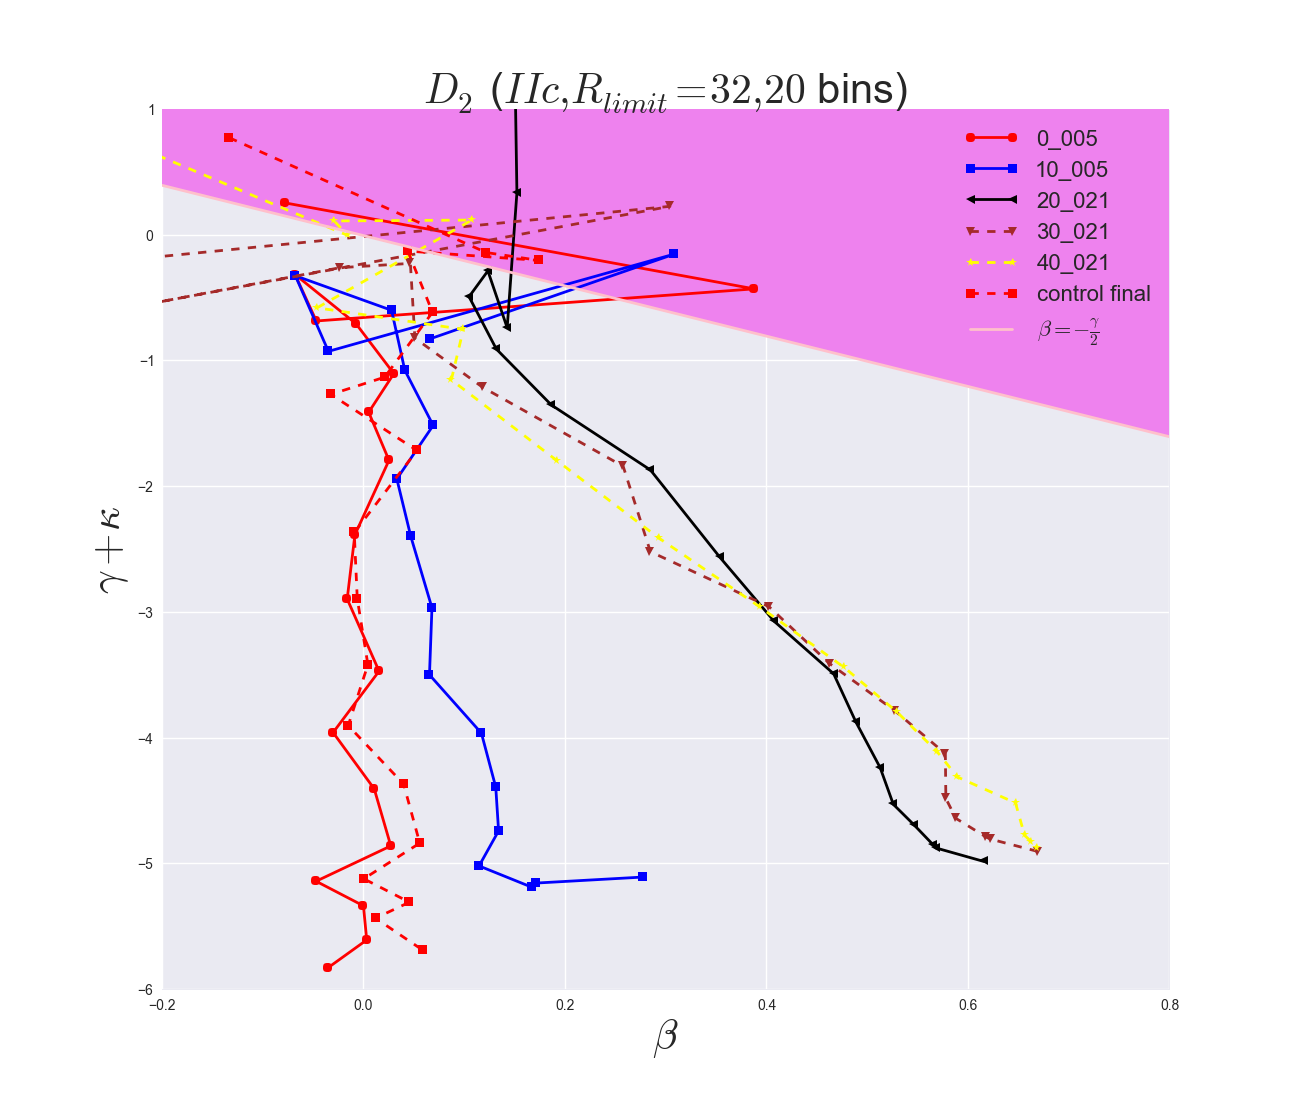
\includegraphics[width=1.0\linewidth]{img/beta_vs_gamma_plus_kappa_IIc_D2_Rlimit32.png}
\caption{$\gamma + \kappa$ vs. $\beta$ for IC, 10, 20, 30, final product and control run of sim. IIc of structure $D_2$. Structures are cut off at a radius of 32 times the scale radius. 20 radial bins are used.
The IC is seen to start out as isotropic ($D_2$ is generated by Eddingtons inversion method) but then systematically exhibits flow toward the same attractor as seen present in the previous figure for the $CS_4$ structure. This structure is given more simulation time than $CS_4$ in order to follow its evolution more fully. It is indeed seen to move closer and closer to the characteristic s-shaped attractor curve found by others [4]. It is therefore safe to conclude that sim. IIc (perturbing tangential velocities) will drive structures towards the attractor previously found.}
\label{fig:test}
\end{figure}

\subsubsection{IId: Energy exchange (speed perturbations)}
\textbf{Using structures $CS_4$ and $D_2$, this simulation perturbs only the speed of particles and not the direction of the velocity vector. Specifically, for all of these structures the total velocities inside spherical bins is perturbed for each of its particles by multiplying those given particles cartesian velocities ($v_x$, $v_y$ and $v_z$) by the same random numbers for each three directions (thus only changing the speed) in the range $[0.7, 1.3]$ (corresponding to perturbing the kinetic energies by random numbers in the range $\frac{1}{2}\cdot[0.49, 1.69]$), taken from the continuous uniform distribution. Following this exchange of kinetic energies between particles in fixed spherical bins, a normalization factor is applied to the total velocities, which ensures energy conservation. it has the same functional form as the one applied in sim. IIa. After these velocity kicks the structures are simulated under their self gravity allowing them to flow a bit under their new velocities. This procedure is then repeated for a total of 20 runs (with one initial run where there is no perturbation. This allows the OM models to reach equilibrium, as they are not perfectly equilibrated when set up as OM models. It is done for Edd structures as well to be certain of equilibrium before any perturbations take effect). After the first 10 runs, the random number range is unchanged but the runs 11 $\rightarrow$ 20 are given longer timespans ($t_{sim} = 500$ corresponding to 5 dynamical times at $r = 12.7r_s$) to allow structures more flow.} \\ \\

\begin{figure}[!htbp]
\centering
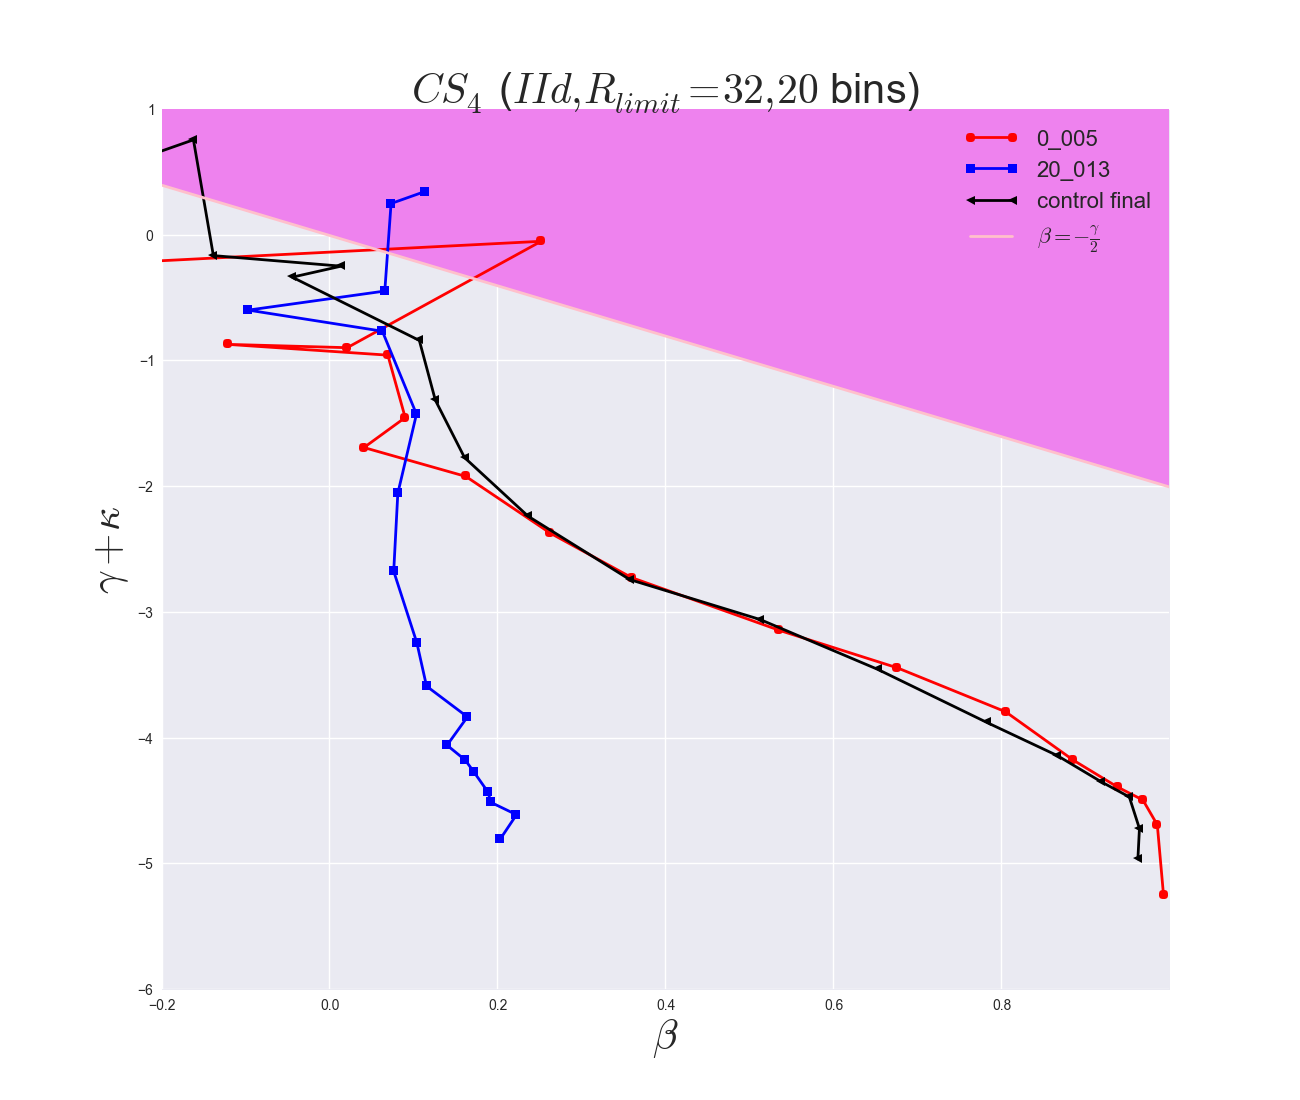
\includegraphics[width=1.0\linewidth]{img/beta_vs_gamma_plus_kappa_IId_CS4_Rlimit32.png}
\caption{$\gamma + \kappa$ vs. $\beta$ for IC and final product of sim. $II_d$ of structure $CS_4$.
Structures are cut off at a radius of 32 times the scale radius. 20 radial bins are used.
The attractor is present and can be seen for the final structure 20$\_$013 which has been driven towards $\beta = 0.1$ in the outer regions. The pink upper right area is found to be an unstable region by An and Evans (2006).The control runs which are simulated with no perturbations interfering can be seen as well. They show no significant departure from the initial conditions.}
\label{fig:test}
\end{figure}

\begin{figure}[!htbp]
\centering
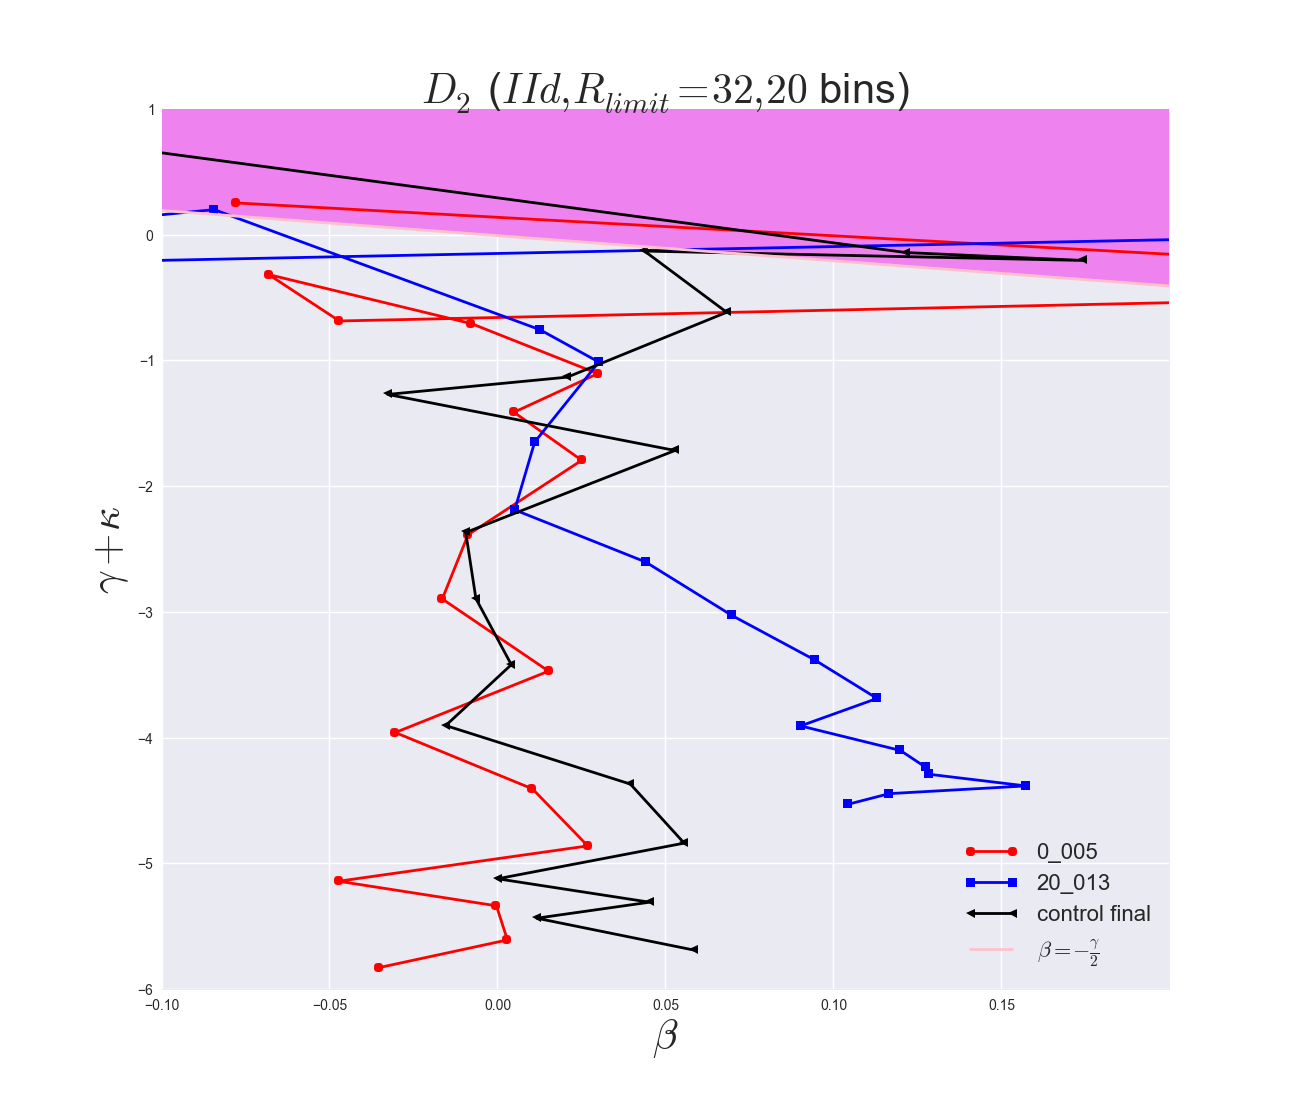
\includegraphics[width=1.0\linewidth]{img/beta_vs_gamma_plus_kappa_IId_D2_Rlimit32.png}
\caption{$\gamma + \kappa$ vs. $\beta$ for IC and final product of sim. $II_d$ of structure $D_2$.
Structures are cut off at a radius of 32 times the scale radius. 20 radial bins are used.
The attractor is present and can be seen for the final structure 20$\_$013 which has been driven towards $\beta = 0.1$ in the outer regions. The pink upper right area is found to be an unstable region by An and Evans (2006).The control runs which are simulated with no perturbations interfering can be seen as well. They show no significant departure from the initial conditions.}
\label{fig:test}
\end{figure}

\textbf{We have so far seen the ICs plugged into sim. I and II and the outcome of this procedure.
The next section highlights a few features from these sims. such as a particles trajectory when tracking it through subsequent snapshots during a simulation, effects found when zooming in on different radial domains, how softening length introduces numerical noise in the inner region leading us to make a inner cut and how outer parts of structures have insufficient time to reach equilibrium due to the large inter-particle distances leading us to make an outer cut. We thus obtain a valid range of trust where all structures can be safely analyzed. The next section concludes with a mention of OM models and their inability to reach any attractor, in good agreement with previous work done by others.}
\newpage
\section{Statistical analysis and results}

\subsection{Time evolution}
In order to determine the necessary amount of \textit{perturbation} $\rightarrow$ \textit{simulation} repetitions the time-evolution is shown for two different structures, namely $CS_4$ and $D_2$. they are tracked from ICs to final products with intermediate snapshots included as well ($10\_005$, $20\_005$ and $30\_005$ ). Here the analysis is based on the type $II_a$ sims. As can be seen from the figures, ten repetitions are sufficient as the structures at this point have become stable. Stable in this context means that continuing the \textit{perturbation} $\rightarrow$ \textit{simulation} experiment will not drastically change the profiles in any way (wrt. $\rho$, $\beta$ etc.). To see the effect of kick and flow independently figure 19 shows structure $CS_4$ at snapshot $19\_005$, then immediately after the next kick at snapshot $20\_000$ and finally after flow for a duration of one dynamical time at snapshot $20\_005$. In conclusion the flow is when changes to the structures become apparent but these changes were initiated at the kick so the two are co-dependent in order for this experiment to work. This teaches us about the scaling of both the size of the kicks and the number of dynamical times optimal for allowing the structures to settle into new stable configurations. As can be seen in the previous section under 
Controlled sim. II, dynamical times were set to either 1, 3 or 5. Kicks were either $5\%$, $20\%$ or $30\%$.

\begin{figure}[!htbp]
\centering
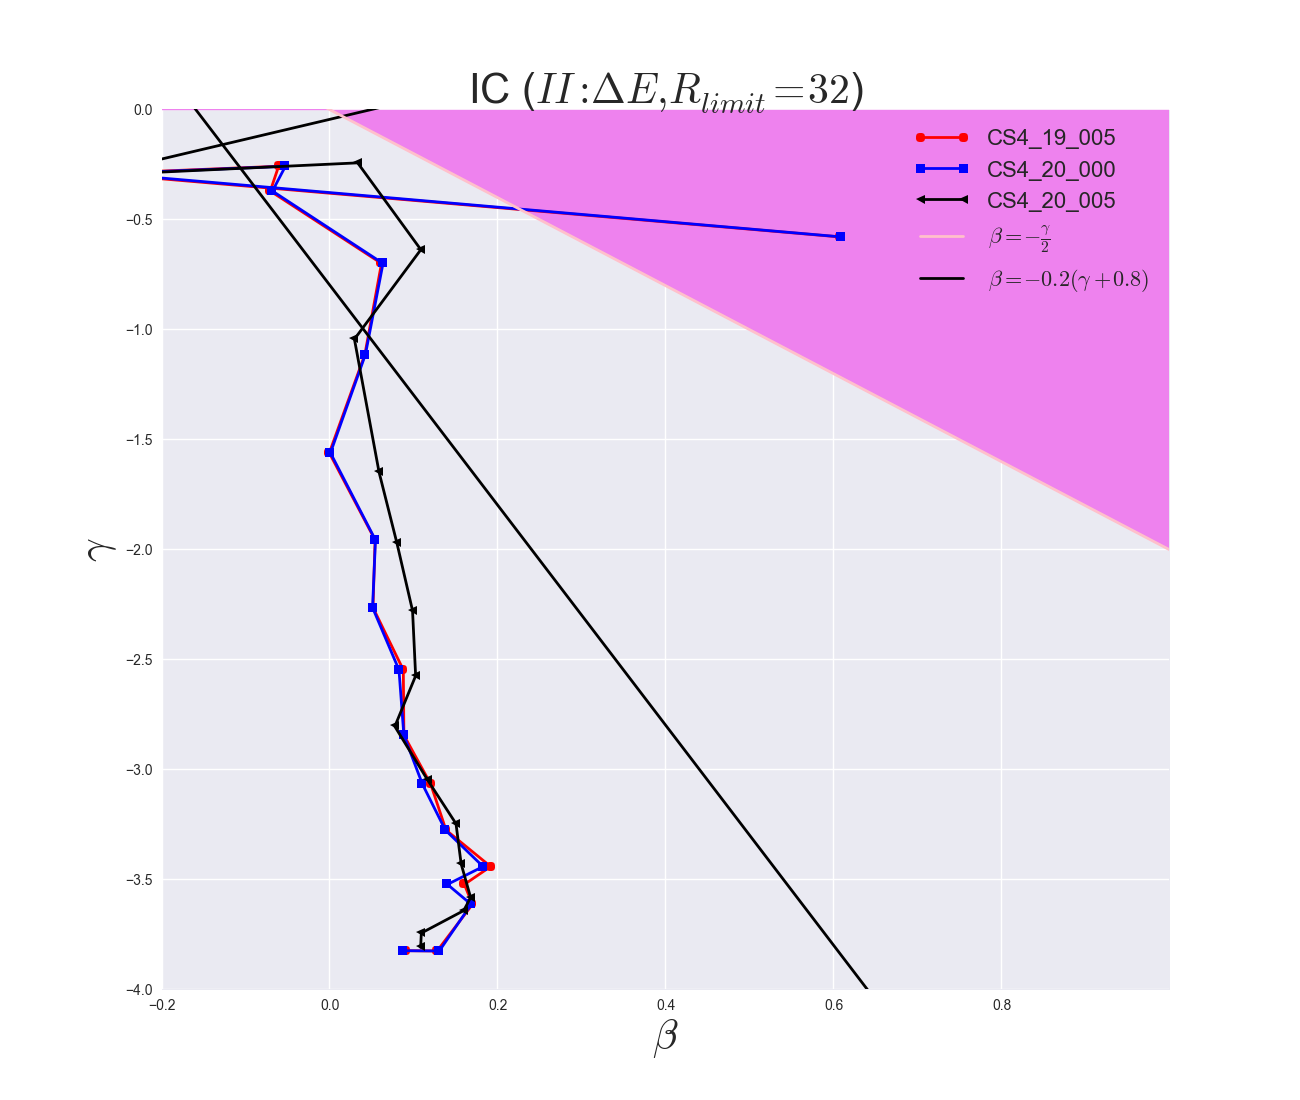
\includegraphics[width=1.0\linewidth]{img/beta_vs_gamma_CS4_Time_evolution_Rlimit32.png}
\caption{$\gamma$ vs. $\beta$ for 19$\_$005, 20$\_$000 and 20$\_$005 of sim. IIa of structure CS4.
Also shown is the linear $\beta$-$\gamma$ relation discovered by Hansen and Moore (2006) for comparison. The pink upper right area is found to be an unstable region by An and Evans (2006). This figure shows us the impact of perturbation and flow independently. Whereas the kick does not change the structure significantly on this type of plot, the subsequent simulation produces substantial alteration. It is thus the combination of both which serves to drive structures towards new equilibria just the same way as violent relaxation and phase mixing have synergestic effects on galaxies during late stages of mergers.}
\label{fig:test}
\end{figure}

\begin{figure}[!htbp]
\centering
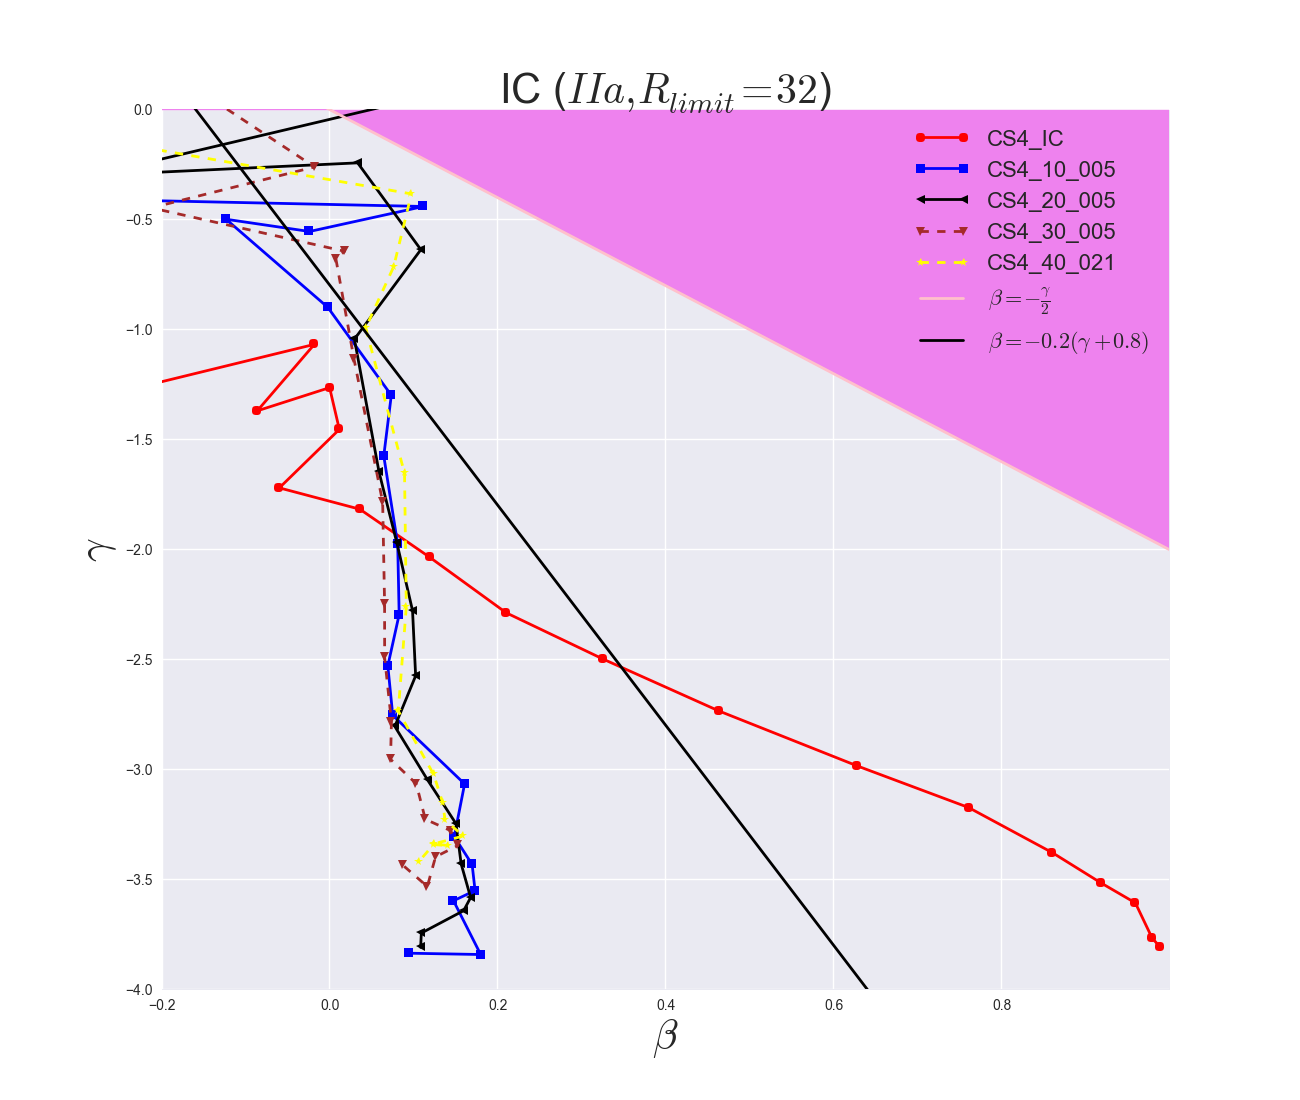
\includegraphics[width=1.0\linewidth]{img/beta_vs_gamma_CS4_Time_evolution_Rlimit32_IIa.png}
\caption{$\gamma$ vs. $\beta$ for IC, 10, 20, 30 and final product of sim. IIa of structure CS4. Also shown is the linear $\beta$-$\gamma$ relation discovered by Hansen and Moore (2006) for comparison. The pink upper right area is found to be an unstable region by An and Evans (2006).
Already after 10 runs the attractor state is present where $\beta = 0.1$ in the outer region.}
\label{fig:test}
\end{figure}

\begin{figure}[!htbp]
\centering
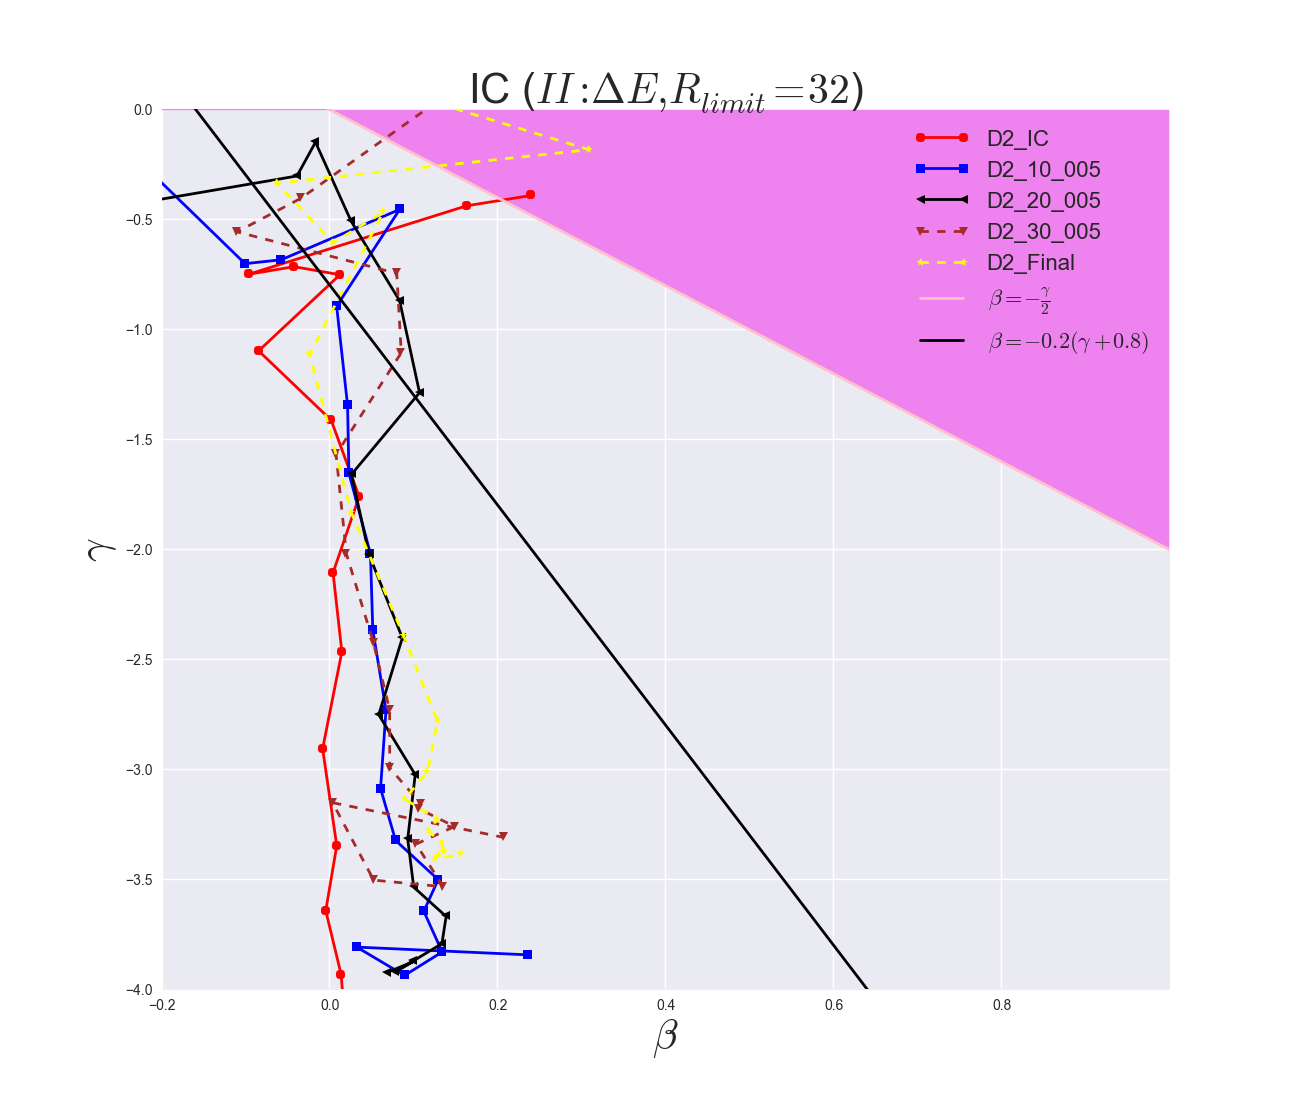
\includegraphics[width=1.0\linewidth]{img/beta_vs_gamma_D2_Time_evolution_Rlimit32.png}
\caption{$\gamma$ vs. $\beta$ for IC, 10, 20, 30 and final product of sim. IIa of structure D2. Also shown is the linear $\beta$-$\gamma$ relation discovered by Hansen and Moore (2006) for comparison. The pink upper right area is found to be an unstable region by An and Evans (2006).
Already after 10 runs the attractor state is present where $\beta = 0.1$ in the outer region.}
\label{fig:test}
\end{figure}

\subsection{Selection of radial domains}
To study local properties of halos more clearly, four distinct regions of structures are plucked out. Radii corresponding to the four $\gamma$-values -1.5, -2.0, -2.5 and -3.0 are taken as central values in bins spanning a with where excactly $10^4$ particles are included. The result of this localized analysis is that the central, majority of particles in structures are well behaved for all sim. in this work (I, $II_a$, $II_b$, $II_c$ and $II_d$) but that the very inner parts are fluctuating due to the approach of gravitational softening length and similarly the very outer parts fluctuates due to insufficient simulation time (the dynamical time at large radii can be very large). See figure 34.


\begin{figure}[!htbp]
\centering
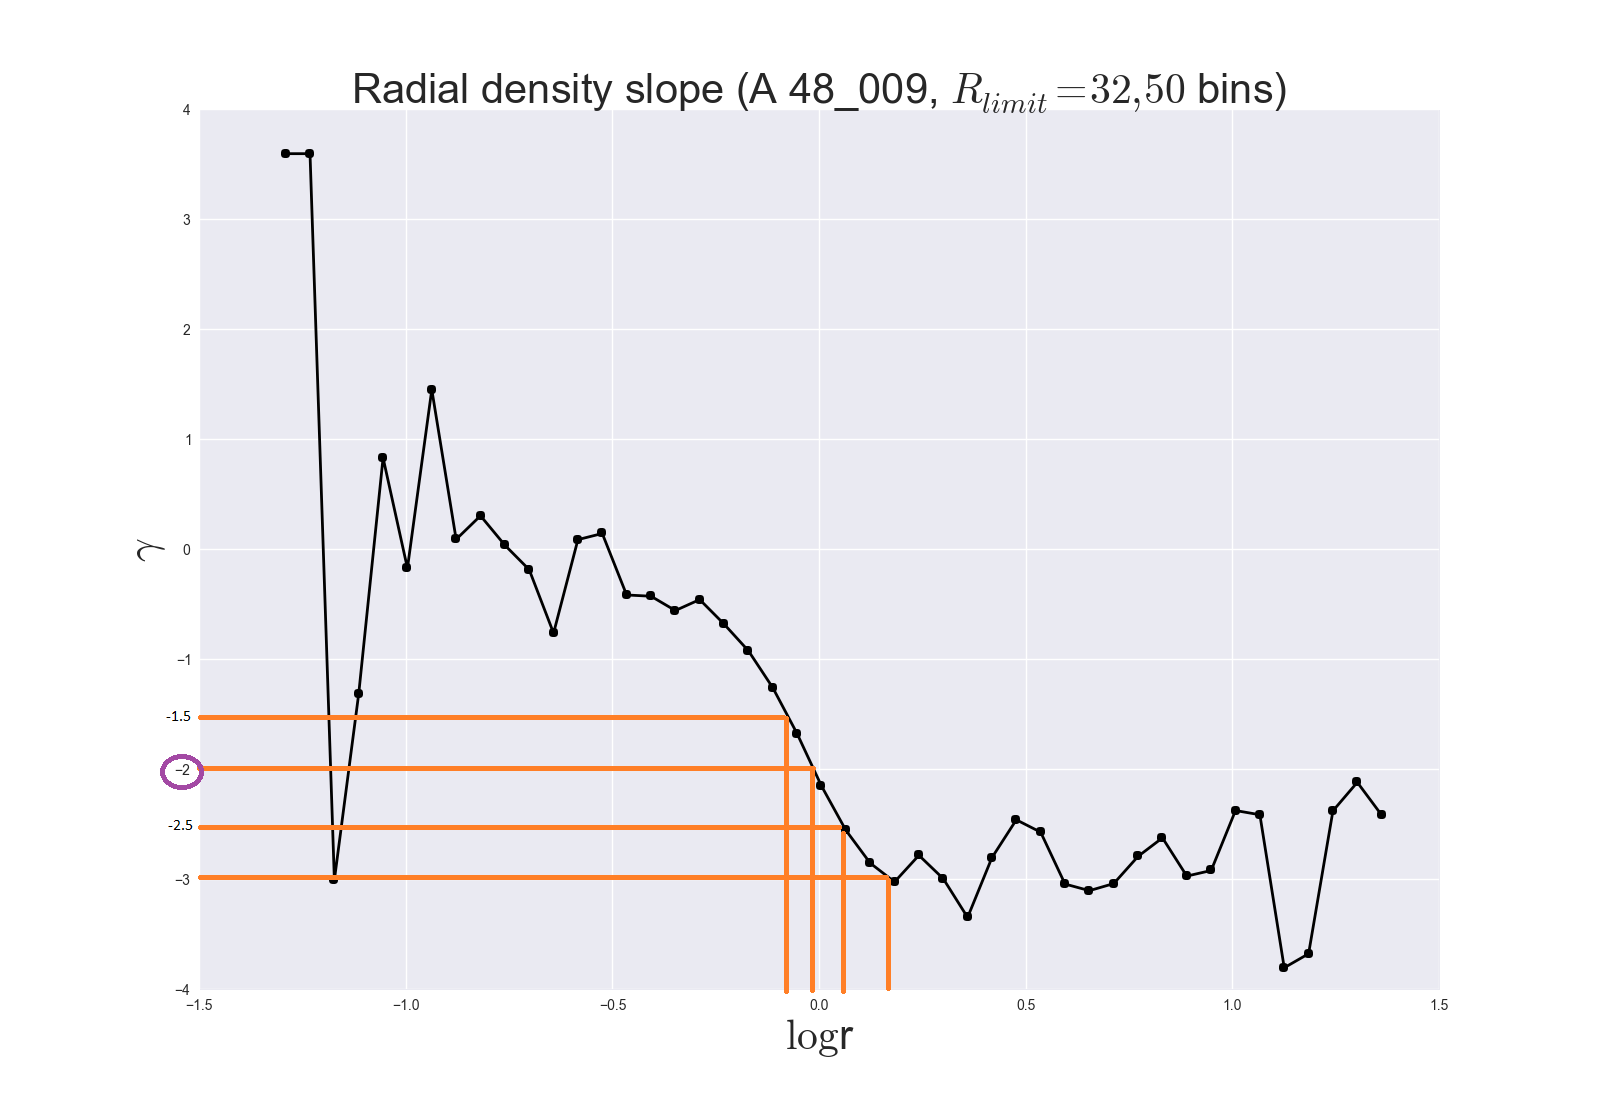
\includegraphics[width=1.0\linewidth]{img/A_48_009_gamma_logr_I_R32.png}
\caption{$\gamma$ vs. $\log r$ for final product of sim. I of structure A (48$\_$009).
The structure is initially cut off at a radius of $R_{lim} = 32\cdot r_s$ (corresponding to the $log_{10}$ value of 1.5) 
Four $\gamma$-values of interest are chosen (indicated by the horizontal orange lines):
$\gamma = -1.5$, -2, -2.5 and -3,
which correspond to four different $\log$ r values, namely
$\log (r_{-1.5})$, $\log (r_{-2})$, $\log (r_{-2.5})$ and $\log (r_{-3})$ respectively (indicated by the vertical orange lines).
In particular $\gamma = -2$ (marked by a purple ring) is of interest for Hernquist structures as its corresponding $\log (r_{-2})$-value indicates the point where the density slope takes on its mean value.
$r_{-2}$ thus introduces a natural length unit which makes comparison between different Hernquist structures with for example different number of particles more meaningful.}
\label{fig:test}
\end{figure}

\subsection{Cuts and range of trust}
Figure 35-37 shows examples of how cuts are chosen.
Noise in inner and outer regions determines the cutting points for inner and outer cuts
and these cuts are performed for both the $\gamma$ vs. $\log r$ plots, the $\kappa$ vs. $\log r$ plots and the $\beta$ vs. $\log r$ plots. Comparing these three parameter plots with cuts found for each,
the most conservative overall inner and outer cuts are determined and applied to that particular structure. This is done for all structures, and the attractor plot (final products after sim. I plotted as $\gamma + \kappa$ vs. $\beta$) can then be seen for the stable regions of all structures undergoing sim. I.
 This principle is then applied to all simulations (I, $II_a$, $II_b$, $II_c$ and $II_d$). 

\begin{figure}[!htbp]
\centering
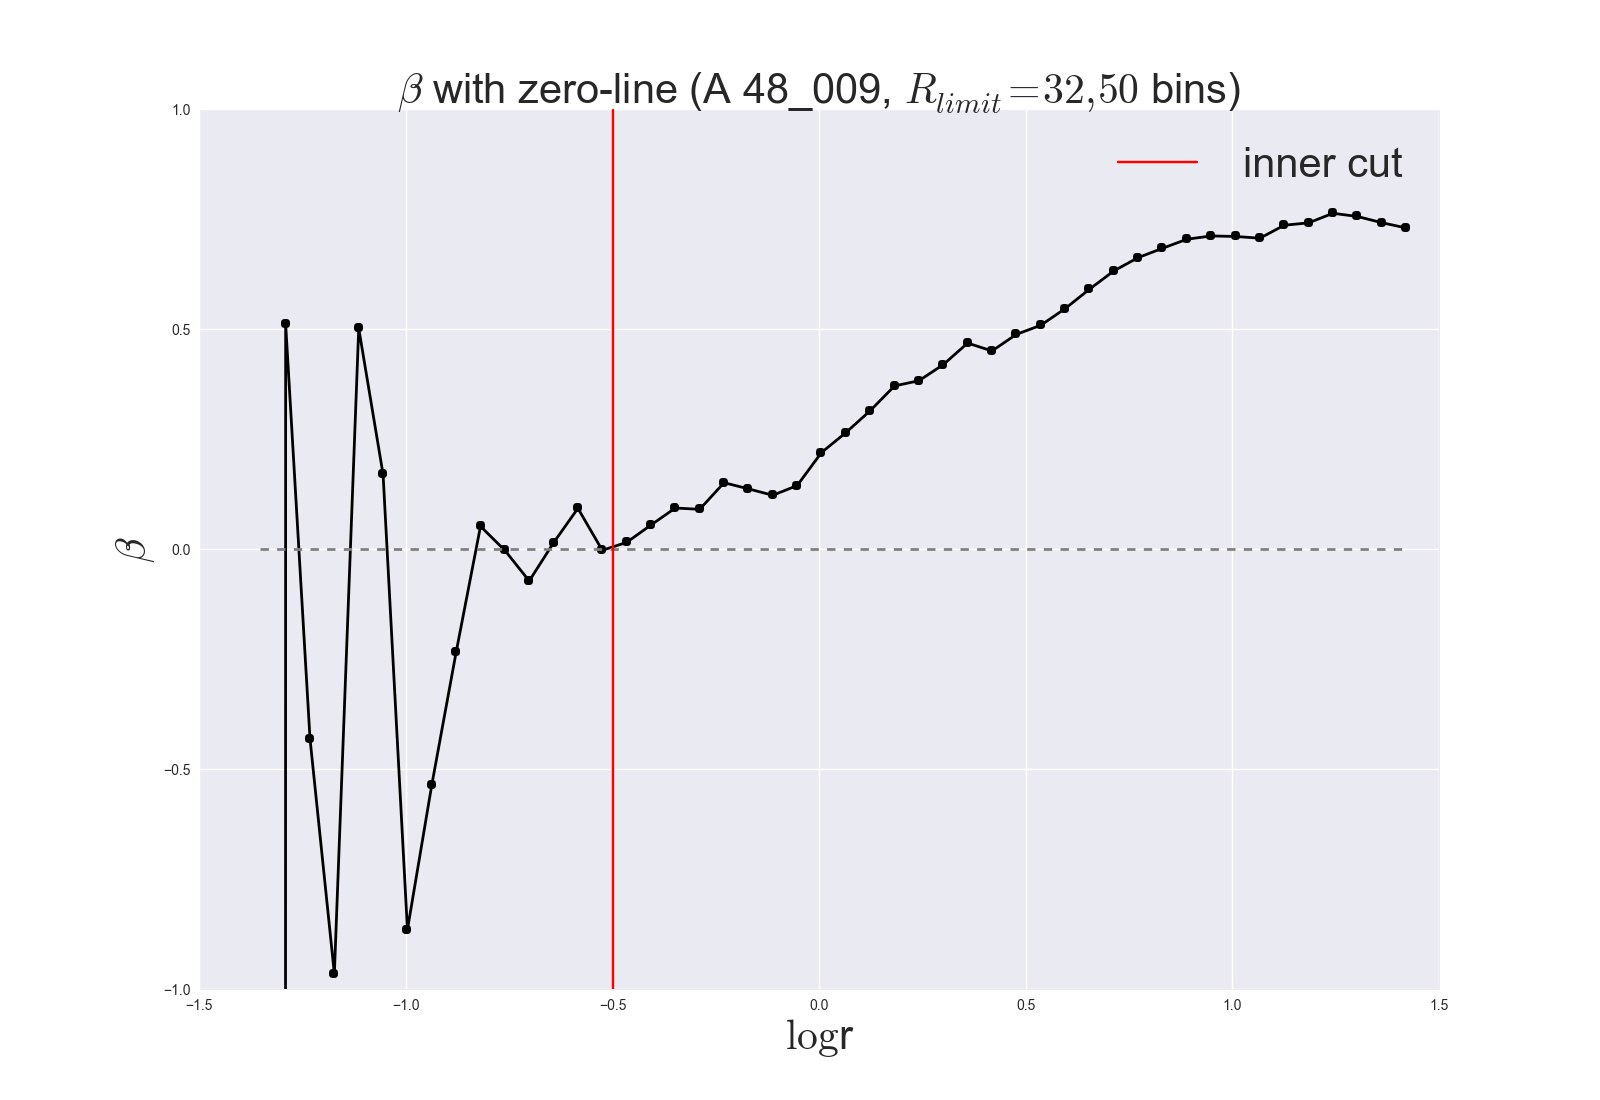
\includegraphics[width=1.0\linewidth]{img/A_48_009_beta_logr_I_R32_cuts.png}
\caption{$\beta$ vs. $\log r$ for final product of sim. I of structure A (48$\_$009).
The structure is initially cut off at a radius of $R_{lim} = 32\cdot r_s$ (corresponding to the $log_{10}$ value of 1.5) 
after which one additional (inner) cut is applied to the $\beta$-profile.
This inner cut (shown in red and located at $\log r = -0.5$) gets rid of Poisson noise due to the discrete nature of the N-body code, 
The remaining points on the $\beta$-profile thus only exist in the $\log r $ interval of [-0.5,1.5], namely the points with numbers [16;48].}
\label{fig:test}
\end{figure}

\begin{figure}[!htbp]
\centering
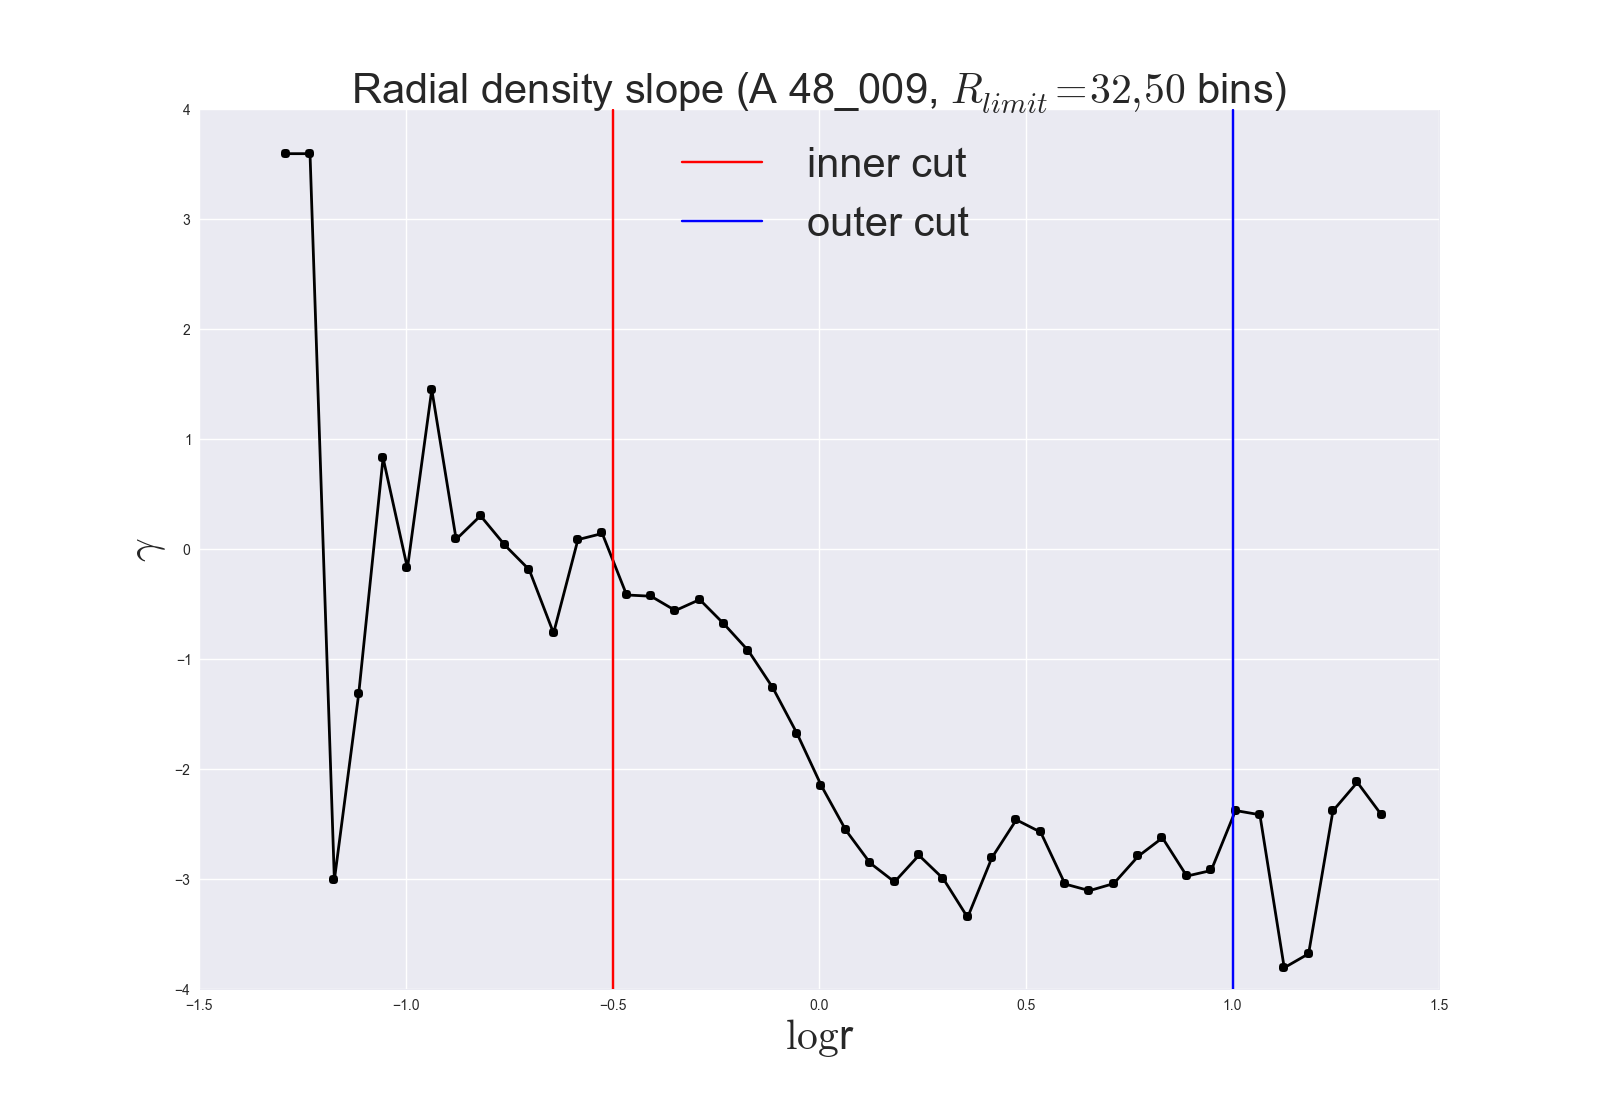
\includegraphics[width=1.0\linewidth]{img/A_48_009_gamma_logr_I_R32_cuts.png}
\caption{$\gamma$ vs. $\log r$ for final product of sim. I of structure A (48$\_$009).
The structure is initially cut off at a radius of $R_{lim} = 32\cdot r_s$ (corresponding to the $log_{10}$ value of 1.5) 
after which two further cuts are applied to the $\gamma$-profile.
The inner cut (shown in red and located at $\log r = -0.5$) gets rid of Poisson noise due to the discrete nature of the N-body code, 
whereas the outer cut (shown in blue and located at $\log r = 1.0$) removes points far away from the halo center, where the particles have not yet had sufficient time to reach a stable equilibrium.
The remaining points on the $\gamma$-profile thus only exist in the $\log r $ interval of [-0.5,1.0], namely the points with numbers [15;39].}
\label{fig:test}
\end{figure}

\begin{figure}[!htbp]
\centering
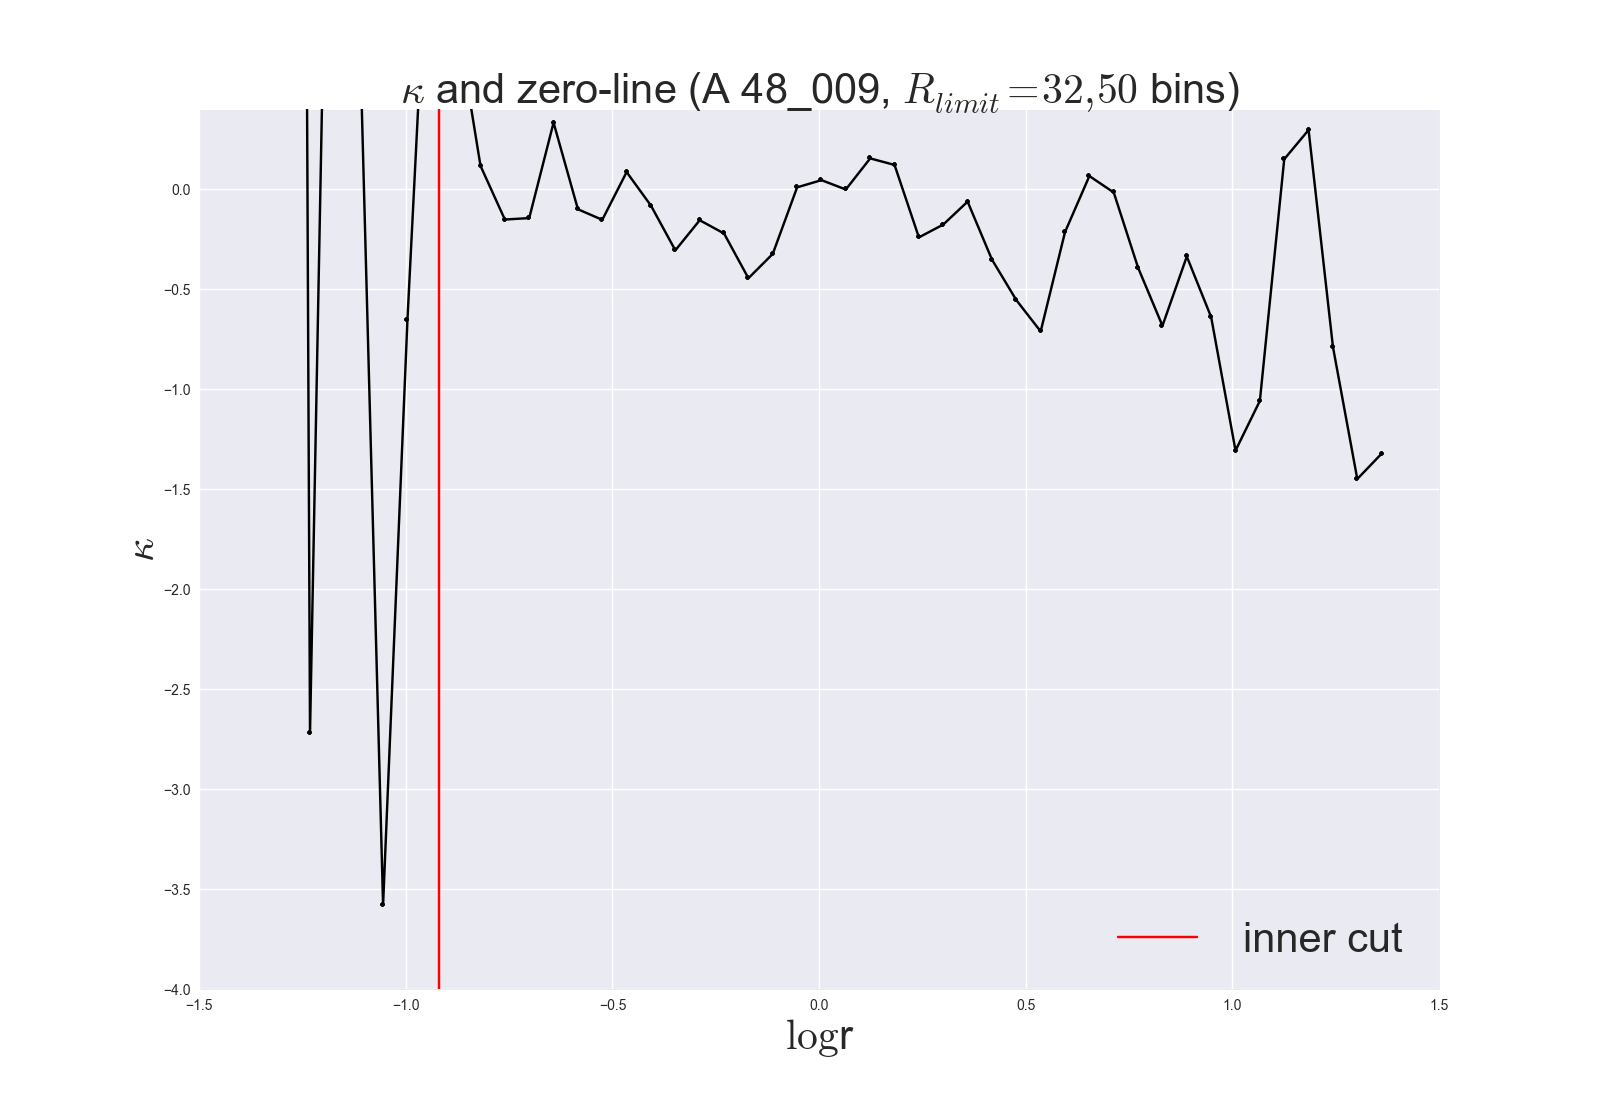
\includegraphics[width=1.0\linewidth]{img/A_48_009_kappa_logr_I_R32_cuts.png}
\caption{$\kappa$ vs. $\log r$ for final product of sim. I of structure A (48$\_$009).
The structure is initially cut off at a radius of $R_{lim} = 32\cdot r_s$ (corresponding to the $log_{10}$ value of 1.5) 
after which one additional (inner) cut is applied to the $\kappa$-profile.
This inner cut (shown in red and located at $\log r \approx -0.9$) gets rid of Poisson noise due to the discrete nature of the N-body code, 
The remaining points on the $\kappa$-profile thus only exist in the $\log r $ interval of [-0.9,1.5], namely the points with numbers [8;46].}
\label{fig:test}
\end{figure}

\begin{figure}[!htbp]
\centering
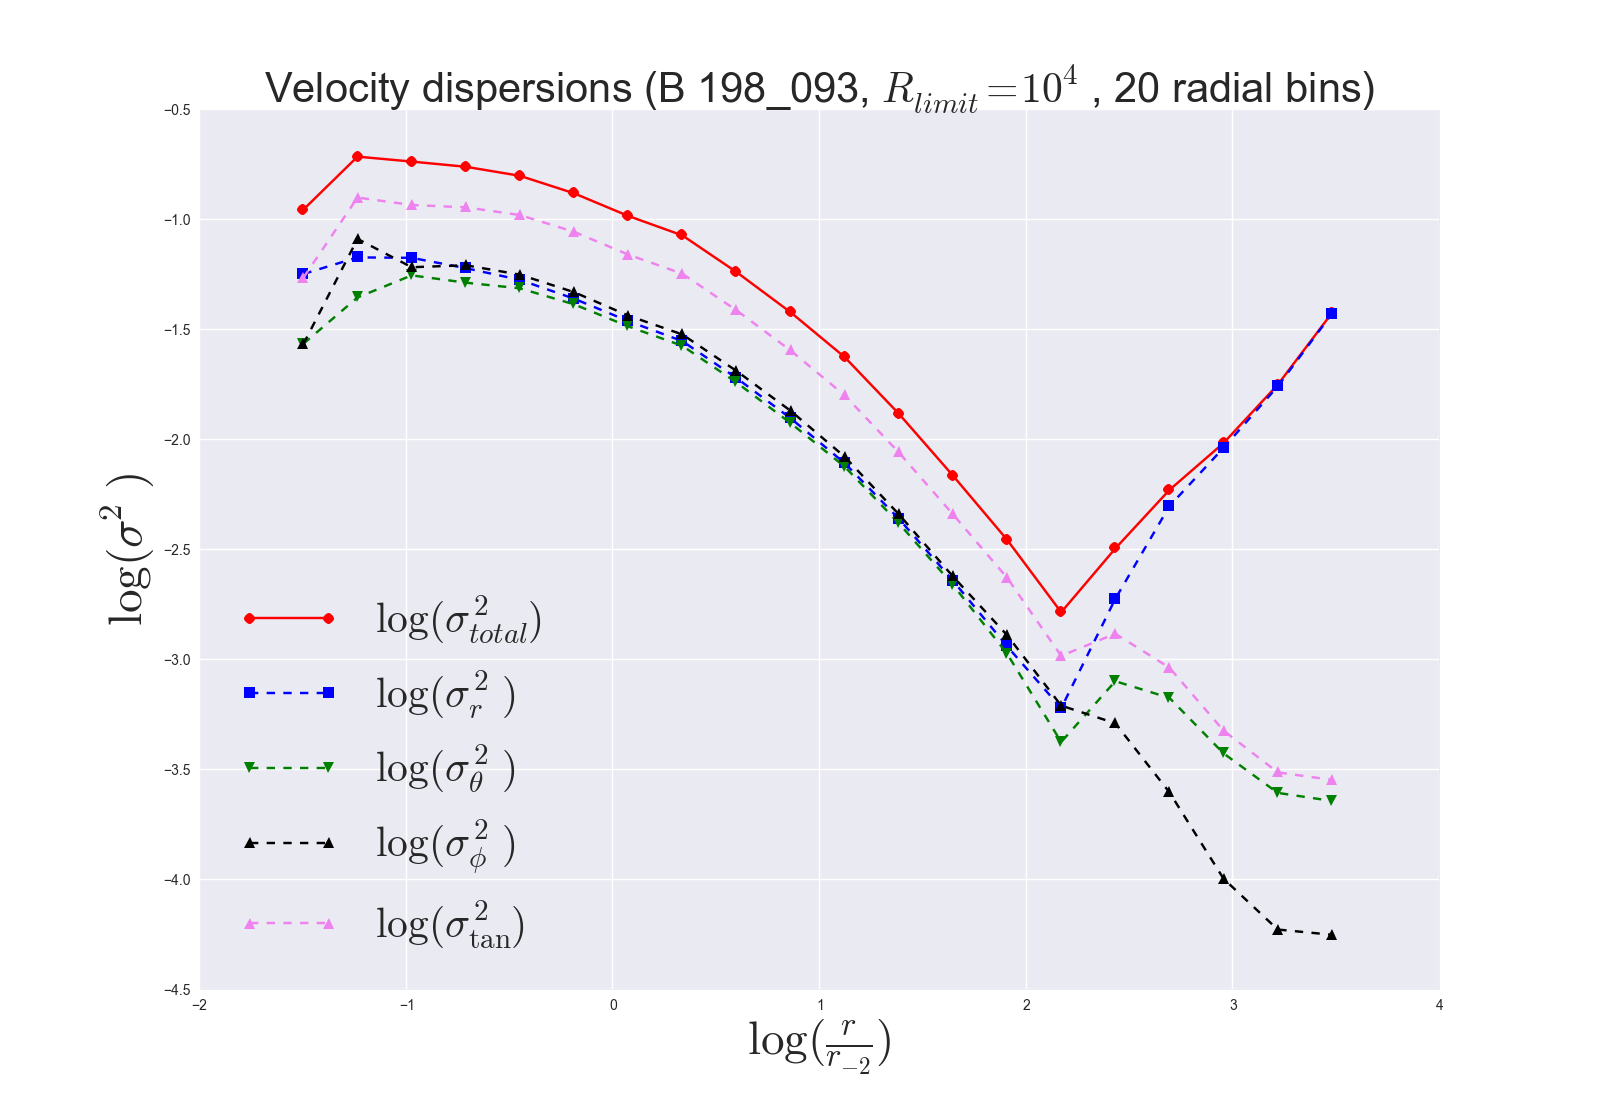
\includegraphics[width=1.0\linewidth]{img/B_198_093_sigma_r_2.png}
\caption{$\log (\sigma^2)$ vs. $\log (\frac{r}{r_{-2}})$ for one of the final products (198$\_$093) of Sim. I for structure B. 
20 bins logarithmic in radius is used and the structure is cut off at radius $R_{limit} = 10^4$ in arbitrary units of radius.
$\sigma^2$ is calculated as $\sigma^2 = \frac{1}{n}\cdot \sum\limits_{i=1}^n (v_i - <v>)^2$ inside each bin, where n is the number of particles inside a particular bin and <v> is the average velocity inside this bin.
For the inner and middle part of this structure the total dispersion is much greater than the 
radial dispersion and greater than the tangential dispersion, but at large radii (from $\log (\frac{r}{r_{-2}}) \approx 2.3$) it can be seen that the radial part starts to dominate over the tangential part and finally almost the entire total dispersion comes from the radial dispersion whereas the tangential dispersion in the outer part is almost negligible.}
\label{fig:test}
\end{figure}

\subsection{Unstable OM models}
OM models with HQ density profiles are unstable when $r_a < 1.33$, since this will cause radial orbit instability (ROI), creating a central bar structure. Several such structures are created ($C_1 \rightarrow C_6$) plus an additional OM structure with inner and outer density slopes (0,-5), ($D_1$). None of them lands on an attractor in the Jeans parameter space. This is in agreement with [8]. See the previous section 'Overview of structures' for more details concerning these profiles.

\textbf{We have highlighted various features from the simulations in this section and the next part summarizes the most important results for the entire project.}
\newpage
\section{Conclusion}
The $\gamma + \kappa$ vs. $\beta$-plots gives useful insight to the effects of each different simulation types for various ICs. \\
\textbf{Sim. I} clearly reproduced the attractor found earlier [7]. The main difference between this sim. and the one done by others is the increased number of perturbation->simulation repetitions as well as the removal of the few gravitationally unbound particles residing in the outer regions of structures toward the later stages of the simulations. The more numerous experiments done in this way indicates a true attractor which is robust against repeated perturbations->simultions as any true attractor must be (as well as any stable points).  \\ \\

End products of \textbf{sim. $II_a$} landed on a almost vertical curve indicating that this type of sim. drives structures closer to isotropy. This behavior is in agreement with previous results [6]. The structures does not become completely isotropic but are attracted towards a state in the Jeans parameter space where $\beta = 0.1$ in the outer parts. This thus indicate the presence of a new attractor. The reason for this probably resides in the fact that this sim. type is symmetric in velocity kicks whereas previous work had been symmetric in energy kicks (perturbing kinetic energy in the range [0.25,1.75]) [4]. This subtle difference might lead to differences in the VDFs which might then dictate the outcome. \\ \\

\textbf{Sim. $II_b$} does not result in any attractor, as the parturbations and flow have no systematic effect on structures and they are seen to fill up a larger and larger span of the parameter space between $\beta$, $\gamma$ and $\kappa$. Perhaps this is just an artificial type of simulation which does not accurately resemble real physical procecces in the universe. One could try to find systematic features in the flow by providing smaller velocity kicks than the ones here utilized. This is in agreement with [4]. \\ \\

End products of \textbf{sim. $II_c$} landed on the characteristic s-shaped attractor curve. This is in agreement with [4]. \\ \\

End products of \textbf{sim. $II_d$} landed on the same almost vertical curve as the one found in $II_a$ indicating that this type of sim. similarly drives structures closer to isotropy. This is the same outcome as the type $II_a$ sim., which is to be expected as it is basically a subclass of $II_a$. This behavior (approaching isotropy) is in agreement with previous results [6]. Again the new attractor seems present in the outer parts of the end products. \\ \\

A relationship between the velocity anisotropy, the radial slope of the density profile, and the radial slope of the squared velocity dispersion is thus confirmed for stable configurations when undergoing simulations of type I (G-perturbations) and $II_c$ (perturbing tangential velocities).
This relationship exists in the form of a one-dimensional attractor (s-shaped curve). 

\centerline{\textit{concluding the side projects (See appendix B),}} 
\centerline{\textbf{cosmological simulations}} 
The cosmological analysis of dark halos morphology indicates that halo shape generally has slight departures from sphericity and can be either oblate or prolate in cosmological simulations. \\

\centerline{\textbf{VDF}} 
Velocity profiles (or Velocity Distribution Functions) of dark matter halos are seen to depart slightly from Gaussian distributions and to be better fitted by Tsallis power laws (Generalized Gaussian distributions) which are more steep and have flatter tails. \\

\centerline{\textbf{LOS}} 
A comparison is made between 3D structures and their corresponding line-of-sight (LOS) appearance showing that details in fine-structure is lost when going from the former to the latter. This is a complication related to observations that does not exist for simulations where a complete 3D view can be obtained.

\centerline{\textbf{Bumpy road to universalities}} 
The radial slope of the density profile is seen to converge towards a characteristic shape with 6 extrema, i.e. 3 maxima and 3 minima. To analyse these features in more detail, each extremum can be applied in turn as a normalization to various structures to see their agreement with, or departure from this, in a closer look. \\ \\

All-in-all an attractor is found alongside other universal trends and it is therefore concluded that the results of structure formation and evolution is not completely random but follow deep underlying physical principles. There must be some physical reason behind this type of behavior as it has been found for a large span of ICs undergoing different types of sims. resembling physical processes taking place during galaxy mergers. The velocity distributions of DM needs to be understood in more detail or understanding the effects of violent relaxation and phase mixing better might give new clues. Hansen, Juncher and Sparre (2010) suggests that this attractor is fundamental for spherical dark matter structures and that it might be seen as a fundamental relation for dark matter; just as the NFW-profile (maybe the attractor can help in explaning why the NFW profile is universal.) and the $\frac{\rho}{\sigma^3}$-relation. The attractor is at least one more interesting feature of our universe concerning dark matter, which might lead to new understanding in the cosmological context. Putting some of the pieces together, we can get closer to solving the Jeans eq.; The density is now modelled, and we have the knowledge of the pseudo-phase-space density as well. Putting these two pieces of information together, this fixes $\sigma_{rad}^2(r)$. In order to determine $\beta$ it still remains to find the tangential velocity dispersion, $\sigma_{tan}^2(r)$. Non-cosmological studies has been conducted to explore the properties of $\beta$-profiles further,e.g. searching for a linear relation between $\beta$ and $\gamma$, which is found in the inner region of cosmological halos. Mass estimates of large structures using the J.E. (derived for a steady spherical system without bulk flow) can be off by up to 40 $\%$ when falsely assuming $\beta = 0$ in some cases. This M-$\beta$ degeneracy (the mass will be different for different choices of $\beta$) could be solved if $\beta$ is known. So for dwarf galaxies for example if $\sigma_r$ and $\rho$ is found then after applying the attractor curve $\beta$ will be known as well thus potentially eliminating the M-$\beta$ degeneracy completely. The J.E. thus effectively removes one degree of freedom from the J.E. \\ 

The advancements in thermodynamics driven by Maxwell and Boltzmann gave a microscopic understanding of universal trends between macroscopic quantities such as pressure, temperature and density for a ideal gas, 
namely by $P = T \cdot \rho$ which lead to the invention of modern statistical mechanics. \\
In terms of DM, finding the relationships between the macroscopic quantities such as density $\rho$, velocity dispersion squared $\sigma^2$ and the velocity anisotropy parameter $\beta$ is where we are at today. Searching for the underlying microscopic physics in terms of VDF's (radial and tangential) will be one of the next steps needed to obtain a more fundamental understanding. \\ \\
In order to be certain if a configuration really represents a true attractor the eigenvalues related to this configuration must be considered. An attractor can have both positive and negative eigenvalues. They are called Lyapunov exponents since we follow them 'around in space' (in this case the 3D Jeans parameter space. They are not calculated in a point). This is a possible next step to test attractors further. In [15] the flow towards the attractor found in [4] is examined and it is found that the further away ICs are from this attractor, the faster they will flow towards it. Also the larger the perturbations the larger the flow rate towards the attractor. Structures then slows down as they approach the attractor and are never seen to cross it (in a way that stars would when flowing towards the main sequence attractor found on a HR diagram) thus indicating a damped oscillator type system which could potentially be described by linear equations from which the Lyaponov exponents might be found and examined. It still remains to find the attractor in cosmological halos, which might have to do with the fact that $\beta$ is different along different directions as well as structures not being totally spherical [9]. To see my analysis codes, please visit the following web-adress: \\
\url{https://bitbucket.org/dark_knights/darkmatterproject}.
\newpage

\begin{thebibliography}{99}

\bibitem{}  Martin Sparre \emph{Eddington-Code developed for Sparre \& Hansen 2012, JCAP, 07,042 and Sparre \& Hansen 2012, JCAP,10,049},  available at \\
\url{https://github.com/martinsparre/Eddington-Code}.

\bibitem{}  Martin Sparre \emph{Osipkov-Merritt-Code developed for Sparre \& Hansen 2012, JCAP, 07,042 and Sparre \& Hansen 2012, JCAP,10,049},  available at \\
\url{https://github.com/martinsparre/OsipkovMerritt}.

\bibitem{} J. Binney and S. Tremaine, Galactic Dynamics: Second Edition, Princeton University Press, Princeton U.S.A. (2008).

\bibitem{} S.H. Hansen, D. Juncher and M. Sparre, An attractor for dark matter structures, arXiv:1005.1643 [INSPIRE].

\bibitem{} S.H. Hansen and B. Moore, A Universal density slope - velocity anisotropy relation for relaxed structures, New Astron. 11 (2006) 333 [astro-ph/0411473] [INSPIRE].

\bibitem{} S.H. Hansen and J. Stadel, The velocity anisotropy-density slope relation, JCAP 05 (2006) 014 [astro-ph/0510656] [INSPIRE].

\bibitem{} S.H. Hansen and M. Sparre, The behaviour of shape and velocity anisotropy in dark matter haloes, arXiv:1210.2392 [astro-ph.CO].

\bibitem{} A. Meza and N. Zamorano, Numerical stability of a family of Osipkov-Merrit models, arXiv:astro-ph/9707004

\bibitem{} M. Sparre and S.H. Hansen, Asymmetric velocity anisotropies in remnants of collisionless mergers, arXiv:1205.1799 [astro-ph.CO]

\bibitem{} V. Springel, The Cosmological simulation code GADGET-2, Mon. Not. Roy. Astron. Soc. 364 (2005) 1105 [astro-ph/0505010] [INSPIRE].

\bibitem{} V. Springel, High perfomance computing and numerical modeling, Lecture 1:
Collisional and collisionless N-body dynamics, 43rd Saas-Fee Course, Star formation in galaxy evolution: connecting numerical models to reality (11-16 March 2013)

\bibitem{} M. Vogelsberger et. al., Dwarf galaxies in CDM and SIDM with baryons: observational probes of the nature of dark matter, arXiv: 1405.5216

\bibitem{} S. Weinberg, Gravitation and Cosmology: Principles and Applications of the General Theory of Relativity, 1972.

\bibitem{} S. Carroll, Spacetime and Geometry: An Introduction to General Relativity.

\bibitem{} J.A. Barber, H. Zhao, X. Wu and S.H. Hansen, Stirring N-body systems: Universality of end states, arXiv:1204.2764 [INSPIRE].

\bibitem{} B. Ryden, Introduction to Cosmology.

\bibitem{} S.H. Hansen, Dark matter density profiles from the jeans equation, Mon. Not. Roy. Astron. Soc. 352 (2004) L41 [astro-ph/0405371] [INSPIRE].

\bibitem{} S.H. Hansen, Might we eventually understand the origin of the dark matter velocity anisotropy?, Astrophys. J. 694 (2009) 1250 [arXiv:0812.1048] [INSPIRE].

\bibitem{} S.H. Hansen and M. Sparre, A derivation of (half) the dark matter distribution function, arXiv:1206.5306 [INSPIRE].

\bibitem{} A.S. Eddington, The distribution of stars in globular clusters, Mon. Not. Roy. Astron. Soc. 76 (1916) 572.

\bibitem{} L. Hernquist, An analytical model for spherical galaxies and bulges, Astrophys. J. 356 (1990) 359.

\bibitem{} Power et. al., The inner structure of $\Lambda$CDM haloes - I. A numerical convergence study (2003)

\bibitem{} G. C. Rasmussen, Computational Astrophysics: Structures of dark matter halos around galaxy clusters, exam report for the course 'Computational Astrophysics' at NBI, UCPH (2015).

\end{thebibliography}
\newpage

% \listoffigures

\begin{appendix}

\section{A note on simulation time}
Most runs of sim. I and all runs of sim. II (for all structures and with Run 0 included) lasts $100\cdot TimeMax$, corresponding to one dynamical time $t_{dyn}$ at a radius $r=12.7 \cdot r_s$. \\
Proof (assuming a HQ profile with $\rho_o = \frac{1}{2\pi}$):
The dynamical time is given by
\begin{equation}
t_{dyn} = \frac{1}{\sqrt{G \bar{\rho}}} = \frac{1}{\sqrt{G \cdot \frac{M(r)}{\frac{4}{3}\pi r^3}}} 
\end{equation}
setting G = 1 and inserting the mass-function for a HQ structure, $M(r)=\frac{r_s\cdot r^2}{(1+\frac{r}{r_s})^2}$:
\begin{align*}
& \frac{1}{\sqrt{\frac{ \frac{r_s\cdot r^2}{ (1+\frac{r}{r_s})^2 } }{\frac{4}{3}\pi r^3}}} = \\
& \sqrt{ \frac{\frac{4}{3}\pi r^3}{\frac{r_s\cdot r^2}{ (1+\frac{r}{r_s})^2 } }}     = \\
& \sqrt{ \frac{\frac{4}{3}\pi r^3 \cdot (1+\frac{r}{r_s})^2}{r_s\cdot r^2}}     = \\
& \sqrt{ \frac{\frac{4}{3}\pi r \cdot (1+\frac{r}{r_s})^2}{r_s}} 
\end{align*}
and this will equal 100 when 
\begin{align*}
& \sqrt{ \frac{\frac{4}{3}\pi r \cdot (1+\frac{r}{r_s})^2}{r_s}} = 100 \leftrightarrow \\
& \frac{\frac{4}{3}\pi r \cdot (1+\frac{r}{r_s})^2}{r_s} = 10^4 \leftrightarrow \\
& \frac{r \cdot (1+\frac{r}{r_s})^2}{r_s} = \frac{3\cdot 10^4}{4\pi}\\
\end{align*}
substituting $ r = x\cdot r_s$ we find
\begin{align*}
& x(1+x)^2 = \frac{3\cdot 10^4}{4\pi} \leftrightarrow \\
& x \simeq 12.7
\end{align*}
and so 100 simulation times (TimeMax $= 100$) equals one dynamical time $t_{dyn}$, at $ r = 12.7\cdot r_s$.
\section{Side projects}

\subsection{Cosmological SIMS}
\textbf{Using the Gadget-2 code, two cosmological simulations with $128^3$ and $256^3$ dark matter particles were run in a cosmological box with a co-moving volume of (10 Mpc$)^3$. Gravitational softenings of 7.4 and 1.8 kpc were used, respectively. The simulations were initiated at $z=63$, and the initial conditions were created with the public N-GenIC code, available at the Gadget website: 
\url{http://www.mpa-garching.mpg.de/gadget/}} \\ \\


\subsection{Velocity distribution functions}
\begin{figure}
\centering
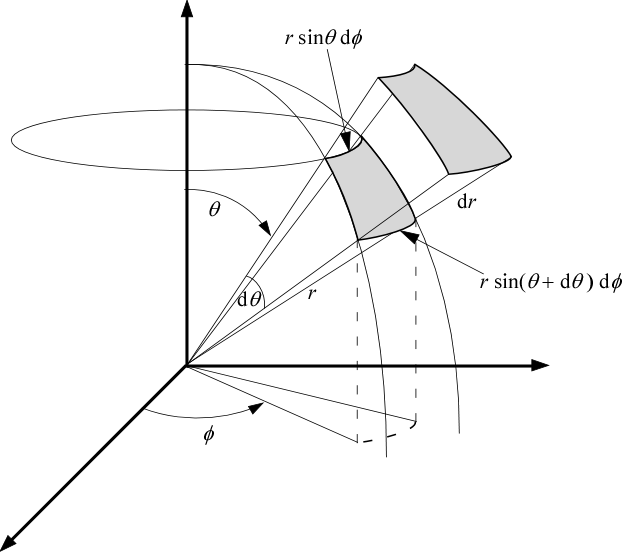
\includegraphics[width=1.0 cm]{img/control-volume-spherical.png}
\caption{Spherical coordinates $ r, \theta $ and $ \phi$. The 3 boldtype coordinate axes represent the Cartesian axes x, y and z. The grey areas shows two small surface areas of concentric spheres around Origo, which together define a small volume element in configuration space. With $ r \geq 0 $, $ \theta \in [0 ; \pi] $ and $ \phi \in [0 ; 2\pi] $ we can define any point in space. credit: http://pleasemakeanote.blogspot.dk/2010/02/9-derivation-of-continuity-equation-in.html}
\label{fig:test}
\end{figure}

Velocity distribution functions (VDF's) are fundamentally important in order to understand the behavior of DM dynamics.

The initial velocity distributions are Gaussian and have velocity dispersions,  $ \sigma_{rad}$  and $\sigma_{tan} $, which I later use in the analysis code (they can be found from the Jeans equation, see previous section). It is worth mentioning that in reality, the velocity distributions is probably not Gaussian but the velocity is anisotropic. The Dark Matter velocity is badly understood, however this will normally not effect the discovery of dark matter in direct experiments. But it is critically important to understand the DM velocity better in order to compare different experiments with each other, as well as comparing direct detections with colliders. So it is crucial to develop a better understanding in order to detect the actual DM particles. 


The total velocity of each particle is decomposed into the 1D radial velocity, and the 2D tangential velocity which can be further decomposed into 
two mutually orthogonal velocity vectors residing in the tangential plane of the halo wrt the radius vector. They are $v_{\theta}$ and $v_{\phi}$.

From the cartesian coordinates, the spherical coordinates can be found: \\
\begin{equation}
\begin{aligned}
&r = \sqrt{x^2+y^2+z^2} \\ 
&\theta = arccos \bigg(\frac{z}{|\boldsymbol{r}|} \bigg)  \\
& \phi = arctan \bigg(\frac{y}{x} \bigg) \\
\end{aligned}
\end{equation}

Similarly,
\begin{equation}
\begin{aligned}
&x = \boldsymbol{r} sin\theta cos\phi \\ 
&y = \boldsymbol{r} sin\theta sin\phi  \\
&z = \boldsymbol{r} cos\theta \\
\end{aligned}
\end{equation}

The total velocity vector can be expressed in terms of Cartesian unit vectors, $\hat{i} , \hat{j}$ and $\hat{k}$, as 
\begin{equation}
     \boldsymbol{v}=\begin{bmatrix}
         v_x \\
         v_y \\
         v_z\\
        \end{bmatrix}
        = v_x\hat{i}+v_y\hat{j}+v_z\hat{k}
\end{equation}
Or wrt the spherical unit vectors , $\hat{r} , \hat{\theta}$ and $\hat{\phi}$, as 
\begin{equation}
     \boldsymbol{v}=\begin{bmatrix}
         \dot{r} \\
         r\dot{\theta} \\
         r\dot{\phi}sin\theta \\
        \end{bmatrix}
        = \dot{r}\hat{r}+r\dot{\theta}\hat{\theta}+r\dot{\phi}sin\theta\hat{\phi}
\end{equation}
So the radial velocity becomes
\begin{equation}
\begin{aligned}
\boldsymbol{v_r} &= \frac{\boldsymbol{r}\cdot \boldsymbol{v}}{|\boldsymbol{r}|} = \frac{x\cdot v_x + y\cdot v_y + z\cdot v_z}{|\boldsymbol{r}|} =\\
& \frac{|\boldsymbol{r}| \cdot sin\theta cos\phi \cdot v_x + |\boldsymbol{r}| \cdot sin\theta sin\phi \cdot v_y + |\boldsymbol{r}| \cdot cos\theta  \cdot v_z + }{|\boldsymbol{r}|} =\\
& sin(\theta)cos(\phi)v_x + sin(\theta)sin(\phi)v_y+ cos(\theta)v_z  \\
\end{aligned}
\end{equation}
the tangential velocity component $ v_{\theta}$ is
\begin{equation}
\begin{aligned}
\boldsymbol{v_{\theta}} &= 
\frac{\frac{d\boldsymbol{r}}{d\theta} \cdot \boldsymbol{v}}{|\boldsymbol{r}|} = \\
&\frac{\frac{d}{d\theta} \cdot (r sin\theta cos\phi)\cdot v_x + 
\frac{d}{d\theta} \cdot (r sin\theta sin\phi)\cdot v_y + 
\frac{d}{d\theta} \cdot (r cos\theta)\cdot v_z}{|\boldsymbol{r}|} = \\
&cos(\theta)cos(\phi)v_x + cos(\theta)sin(\phi)v_y + sin(\theta)v_z  \\
\end{aligned}
\end{equation}
the tangential velocity component $ v_{\phi}$ is
\begin{equation}
\begin{aligned}
\boldsymbol{v_{\phi}} &= 
\frac{\frac{d\boldsymbol{r}}{d\phi} \cdot \boldsymbol{v}}{|\boldsymbol{r}|} = \\
& \frac{\frac{d}{d\phi} \cdot (r sin\theta cos\phi)\cdot v_x + 
\frac{d}{d\phi} \cdot (r sin\theta sin\phi)\cdot v_y + 
\frac{d}{d\phi} \cdot (z)\cdot v_z}{|\boldsymbol{r}|} = \\
& \frac{d}{d\phi} \cdot (cos\phi) \cdot v_x + 
\frac{d}{d\phi} \cdot (sin\phi)\cdot v_y + 0 = \\
& -sin(\phi)v_x + cos(\phi)v_y  \\
\end{aligned}
\end{equation},
since for the $\phi$-plane, $z = 0$, $\theta = 90 \deg $ and so $ sin\theta = 1$.
and finally the 2D tangential speed is
\begin{equation}
|\boldsymbol{v_{tan}}| = \sqrt{v_{\theta}^2+v_{\phi}^2}  
\end{equation}
In order to better compare different radial bins, each velocity or speed is normalized by dividing them with their corresponding velocity dispersions. These new dimensionless normalized velocities and speeds are denoted by u;
The radial normalized velocity is 
\begin{equation}
\boldsymbol{u_r} = \frac{\boldsymbol{v_r}}{\sigma_r}
\end{equation}
and the tangential normalized speed is 
\begin{equation}
\boldsymbol{u_t} = \sqrt{\boldsymbol{u_{\theta}}^2+\boldsymbol{u_{\phi}}^2}  =      
\sqrt{\bigg(\frac{\boldsymbol{v_{\theta}}}{\sigma_{\theta}} \bigg)^2+\bigg(\frac{\boldsymbol{v_{\phi}}}{\sigma_{\phi}} \bigg)^2} 
\end{equation}
To see how close the VDFs are to being Gaussian, from the plots we can determine the FWHM and use the relation $ FWHM = 2 \cdot \sqrt{2 ln 2} \sigma \approx 2.355 \sigma $, where $\sigma$ is the velocity dispersion.
This value of $\sigma$ can then be compared to the real $\sigma$ that is computed directly.
The ratio $ \frac{\sigma(FWHM)}{\sigma(computed)} \cdot 100 \% $ then gives the offset in pct.

\begin{figure}
\centering
\includegraphics[width=1.0 cm]{img/o.jpeg}
\caption{A standard normal distribution, scaled appropriately for easier comparison with the following velocity histograms.}
\label{fig:test}
\end{figure}

\begin{figure}
\centering
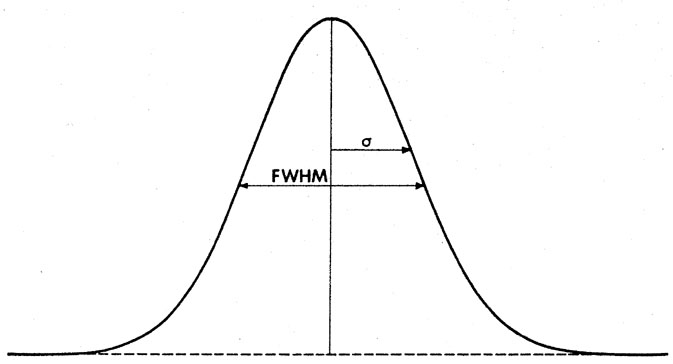
\includegraphics[width=1.0 cm]{img/figure4.jpeg}
\caption{FWHM and $\sigma$ }
\label{fig:test}
\end{figure}

A word on the dispersions: The variance of tangential velocities are defined as $\sigma_{tan}^2 = \sigma_{\theta}^2 + \sigma_{\phi}^2 $,
but this only applies when the angular momentum is the same for all directions wrt the halo centre.
That is easily checked in Python as e.g.

\begin{equation}
\begin{aligned}
L_x &= np.cross(r, v_x) \\
L_y &= np.cross(r, v_y) \\ 
L_z &= np.cross(r, v_z) \\
\end{aligned}
\end{equation}

These quantities are found to be identical.
For a spherical system of gas particles, the radial VDF would read
\begin{equation}
f(\boldsymbol{v_r}) = \exp (-\frac{\boldsymbol{v_r}^2}{2\sigma_r^2})
\end{equation}
and the tangential VDF would be
\begin{equation}
f(\boldsymbol{v_t}) = \boldsymbol{v_t} \cdot \exp (-\frac{\boldsymbol{v_t}^2}{2\sigma_t^2})
\end{equation}

The DM particle velocities is compared with two different fits: a Gaussian function $ a\cdot e^{-b\cdot x^2} $ and a more general power-law fitting function, f(q).
Figure 1 shows a comparison of a standard normal distribution function with f(q):

\begin{figure}
\centering
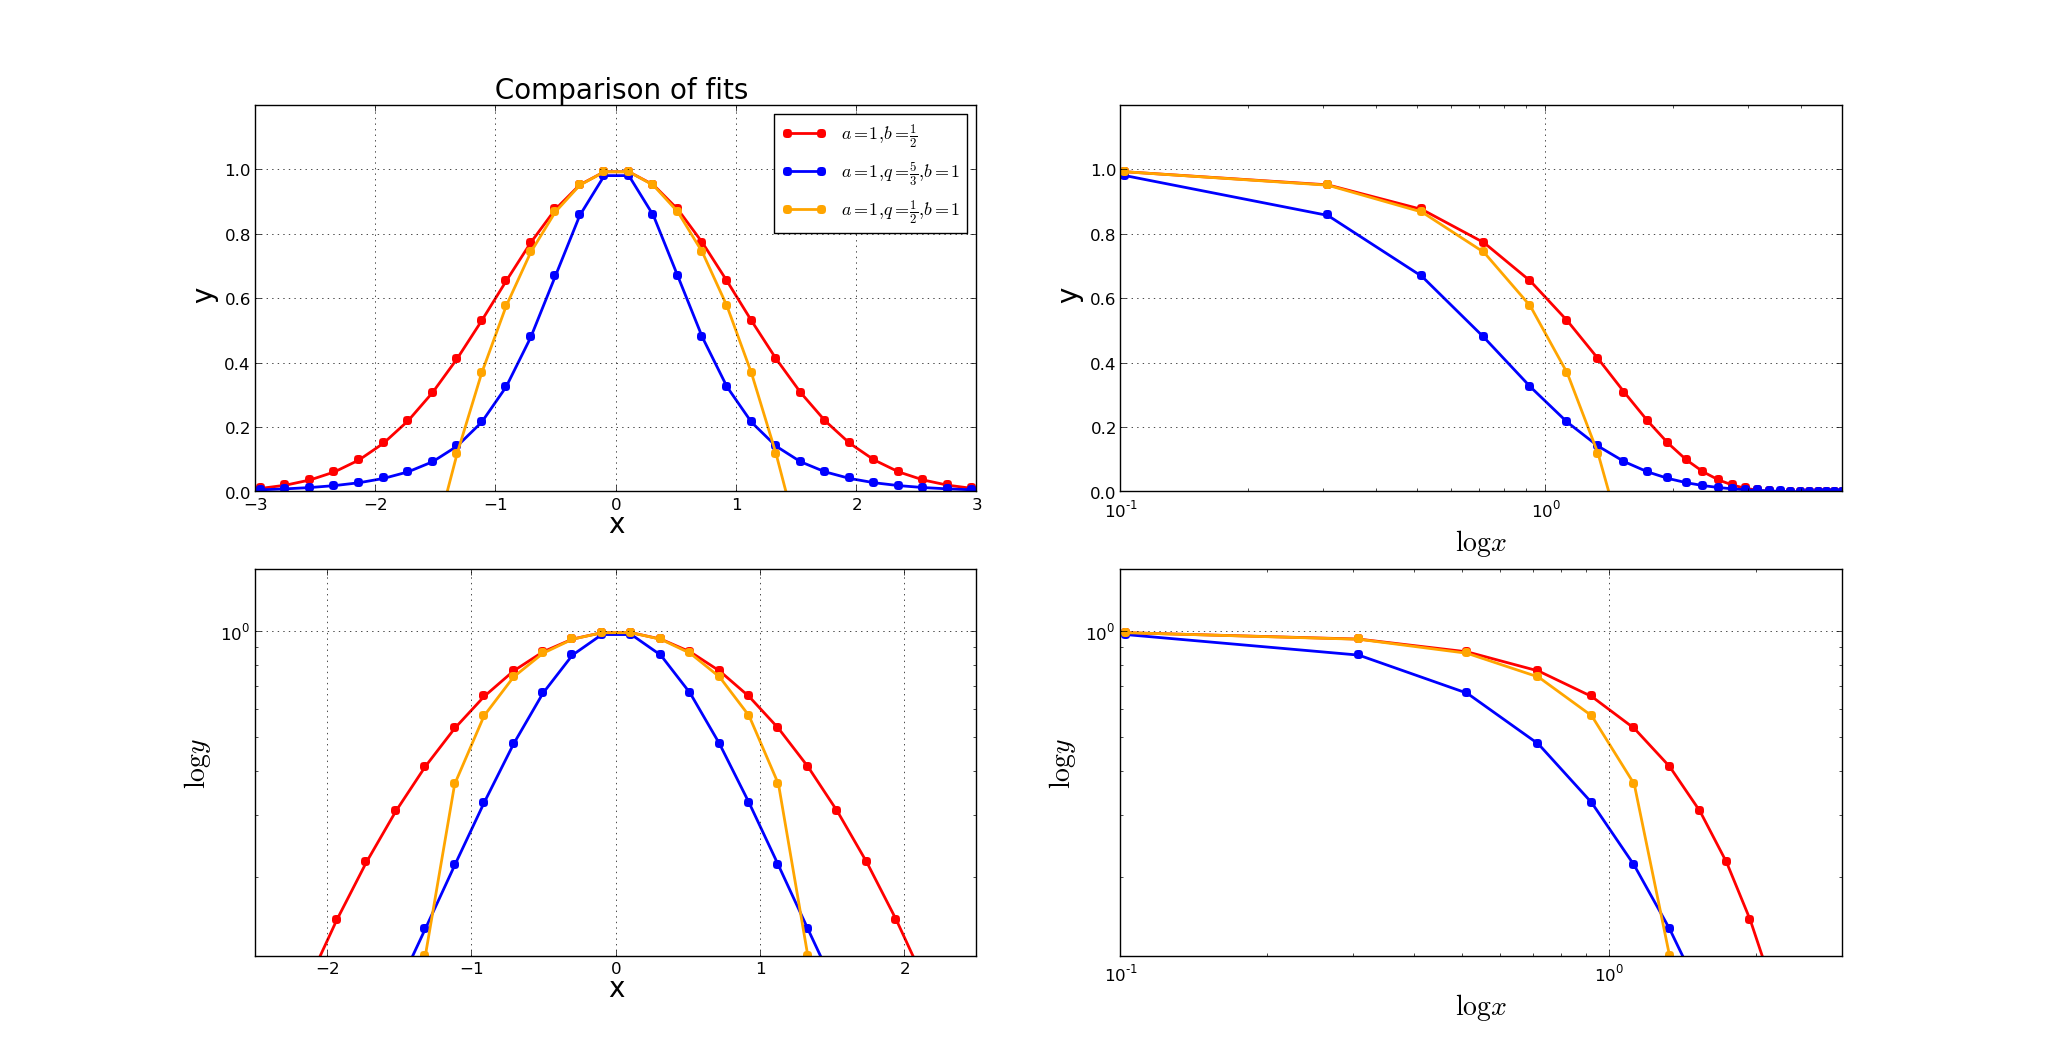
\includegraphics[width=1.0\linewidth]{img/fitcomparison.png}
\caption{$ a\cdot e^{-b\cdot x^2} $ and f(q) for $ q = \frac{5}{3}$ and $ q = \frac{1}{2}$.}
\label{fig:test}
\end{figure}

f(q) and $ae^{-bx^2}$ are both good fits to $v_{tan}$ around $\gamma = -2.0$, which is seen in figure 2:

% Tangential velocities only:
\begin{figure}
\centering
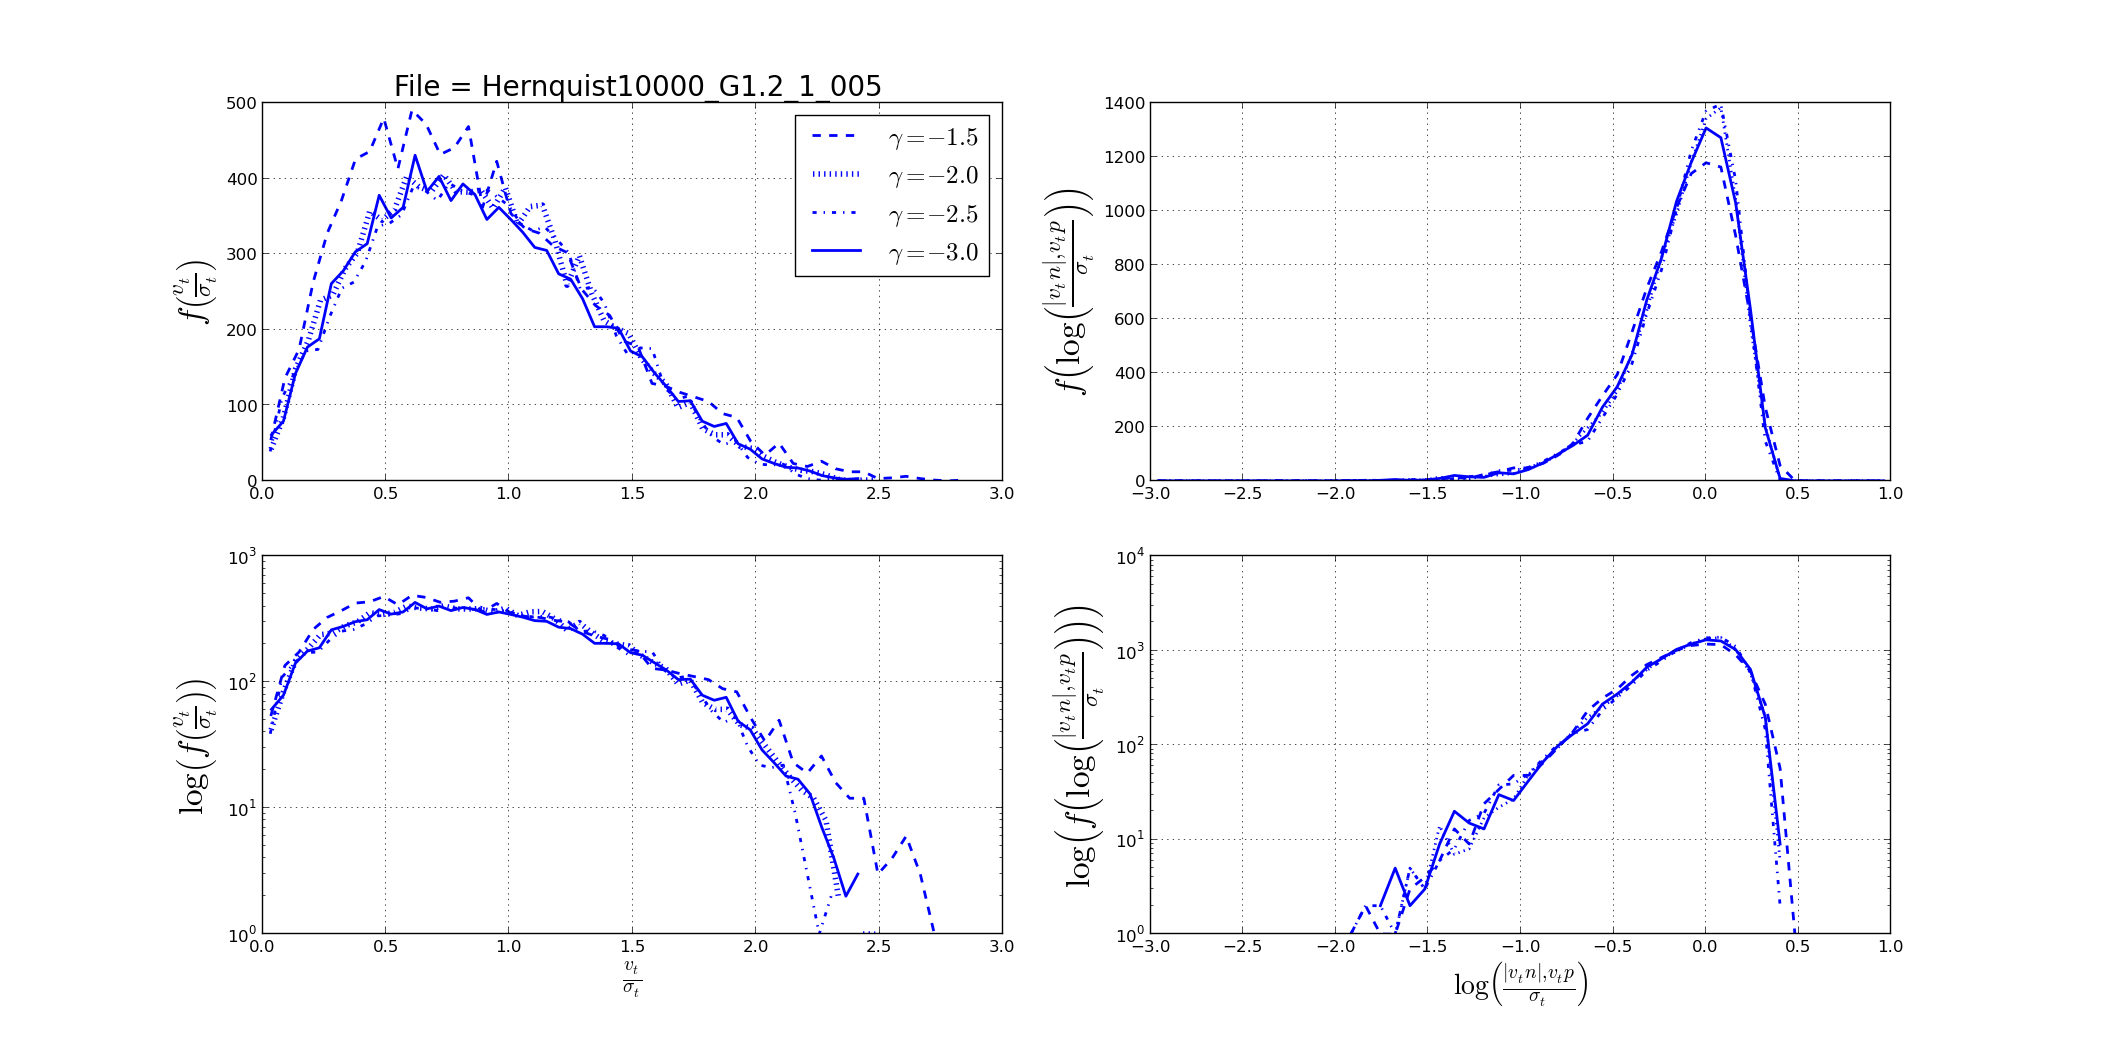
\includegraphics[width=1.0\linewidth]{img/2.png}
\caption{$v_{tan}$ divided by $\sigma_{tan}$, for 4 different radial bins. Shown in lin-lin, lin-log, log-lin and log-log}
\label{fig:test}
\end{figure}

\begin{figure}
\centering
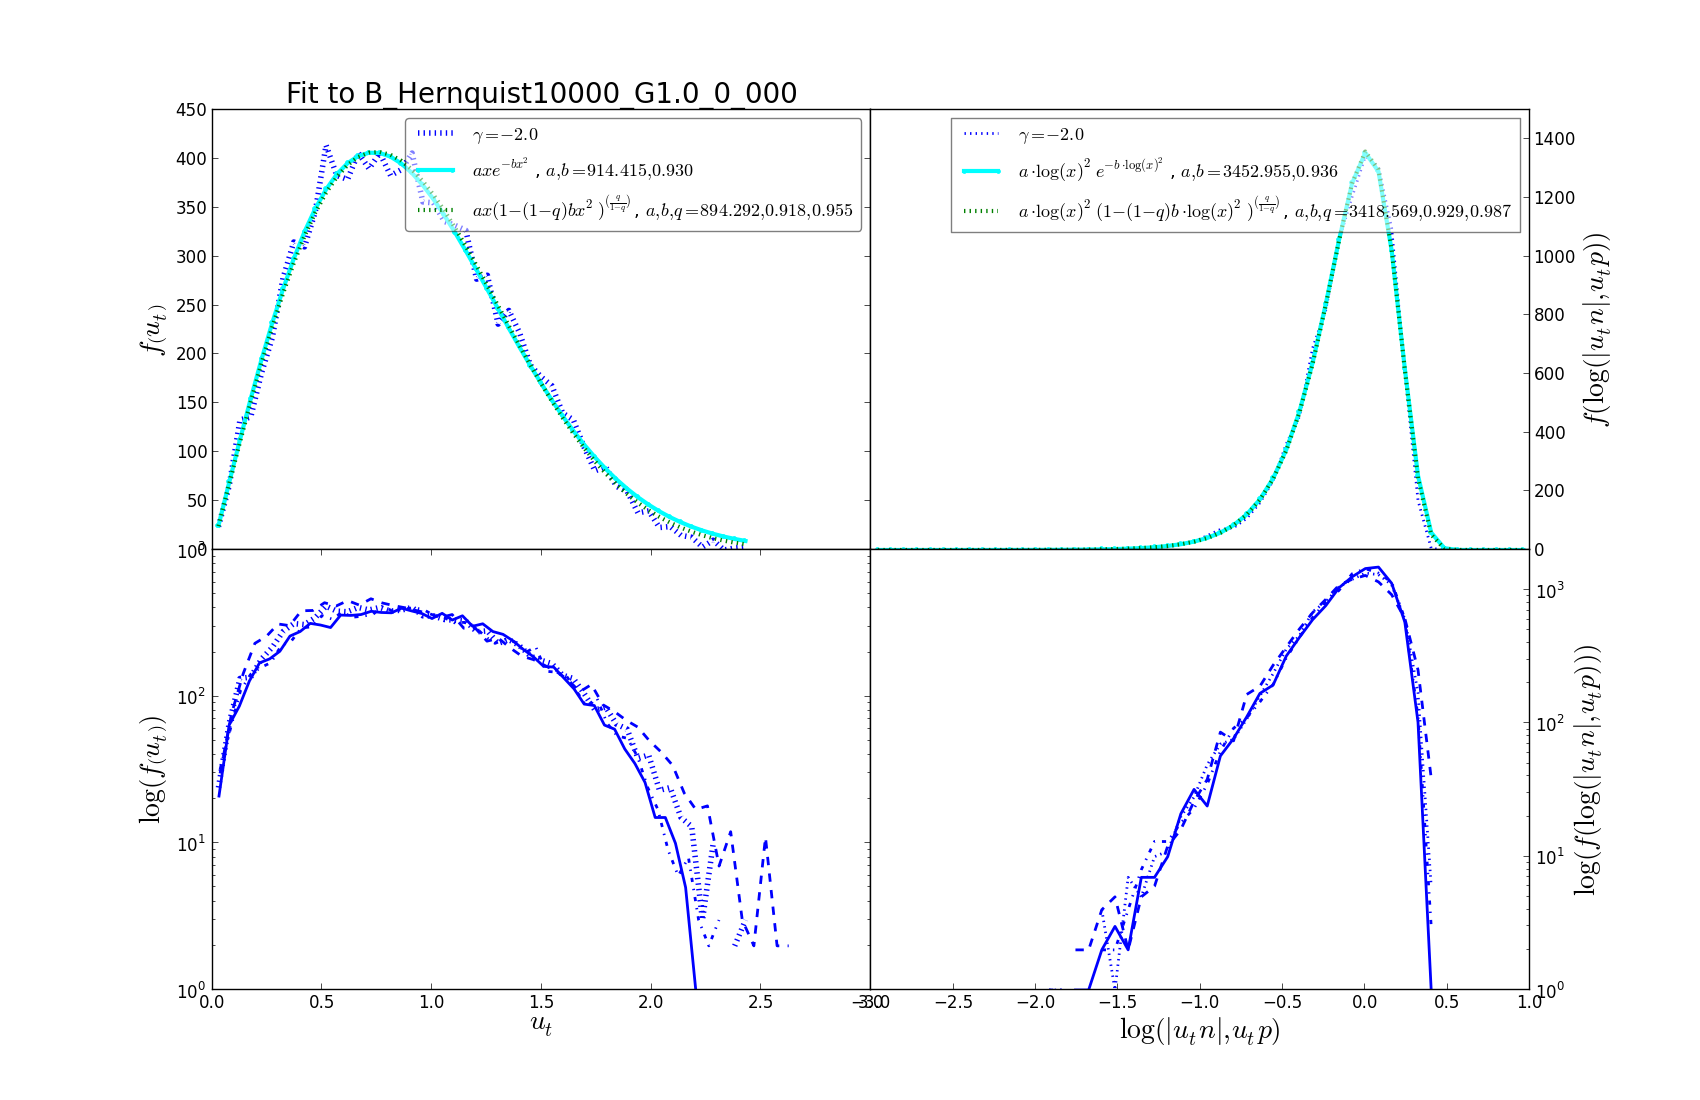
\includegraphics[width=1.0\linewidth]{img/vt_fit_show_abq.png}
\caption{$v_{tan}$ together with Gaussian and Tsallis fit.}
\label{fig:test}
\end{figure}

\begin{figure}
\centering
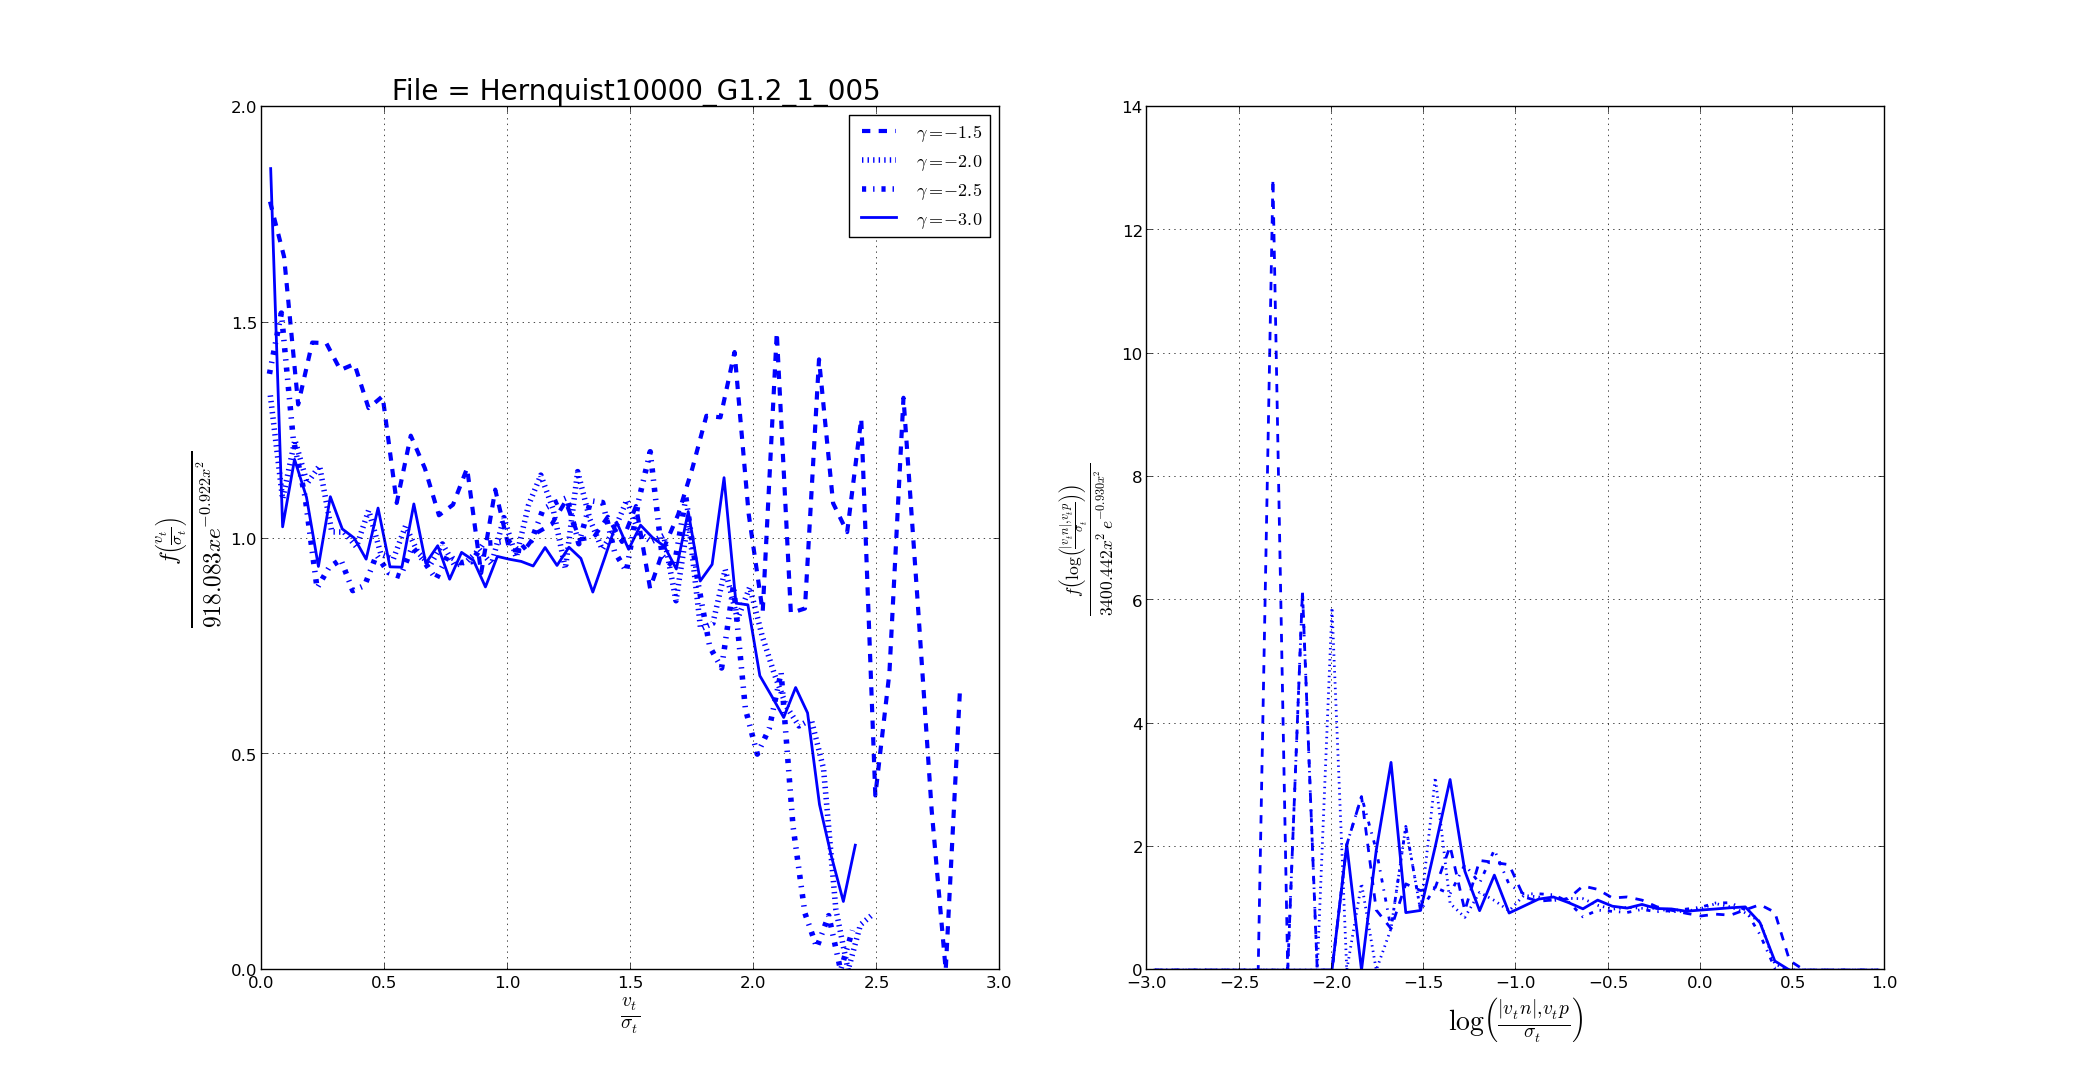
\includegraphics[width=1.0\linewidth]{img/func_guess_vt.png}
\caption{$v_{tan}$ divided by Gaussian function.}
\label{fig:test}
\end{figure}

\begin{figure}
\centering
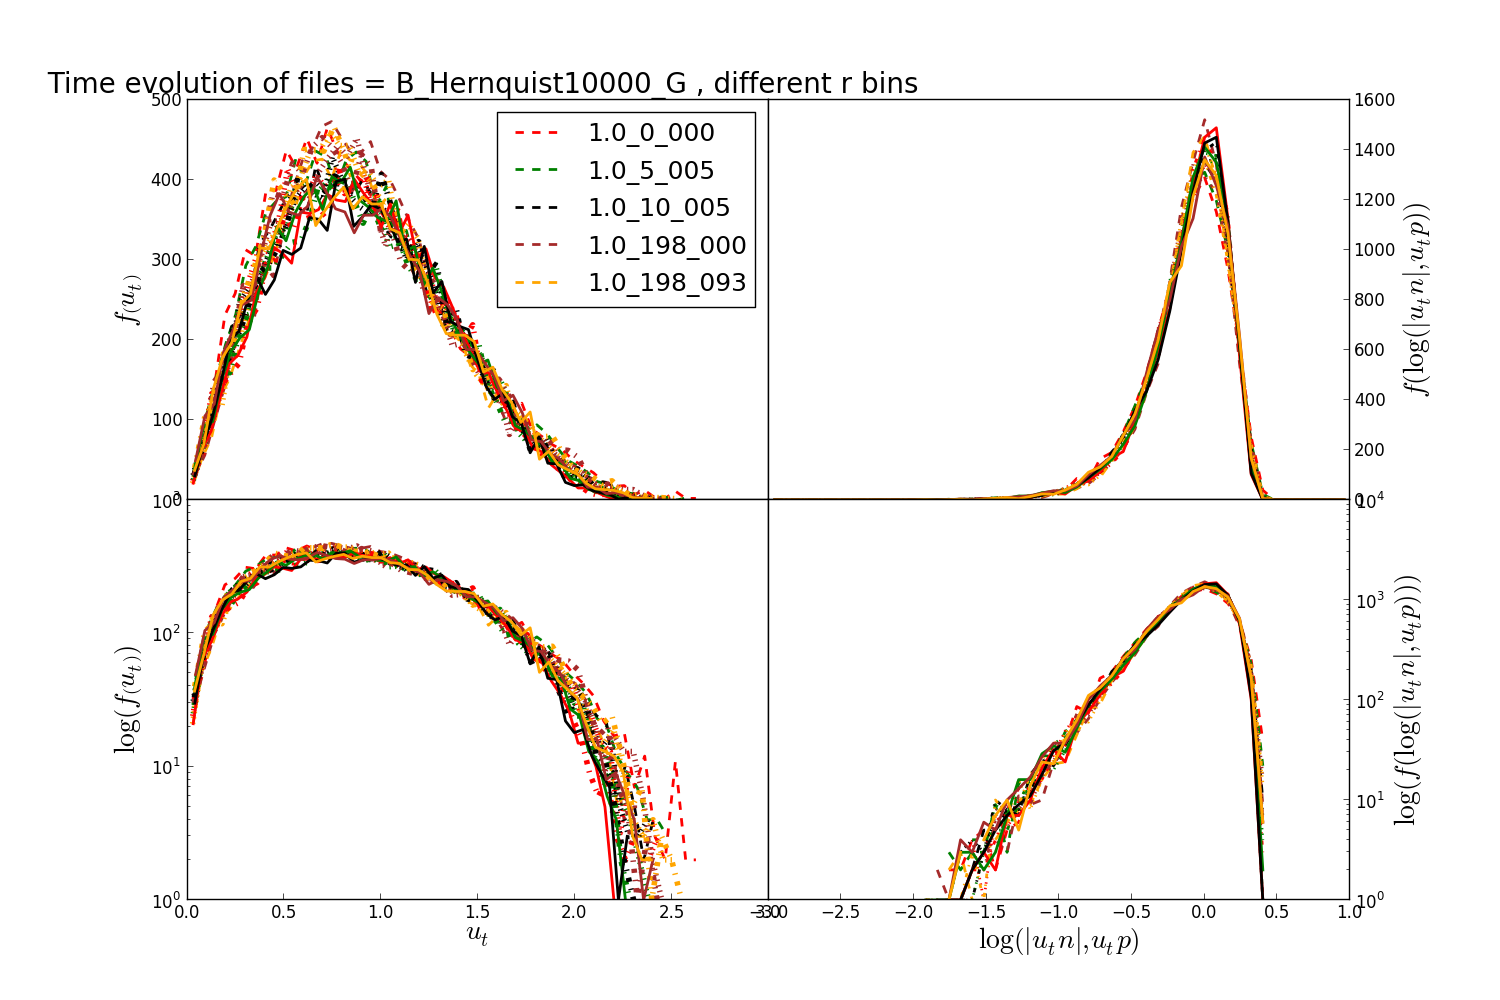
\includegraphics[width=1.0\linewidth]{img/Time_evolution_B_vt_different_rbins.png}
\caption{Histograms of the ratio $ u_t = \frac{v_{tan}}{\sigma_{tan}} $ for 5 different snapshots (this makes it easier to compare different radial bins than it would be for $ v_{tan} $ alone). Data for 4 different radial bins are shown, each containing $10^4$ particles and centered at the radii where $\gamma = -1.5, -2.0, -2.5 $ and $-3.0 $ respectively.}
\label{fig:test}
\end{figure}

% Radial, theta and phi velocities:

\begin{figure}
\centering
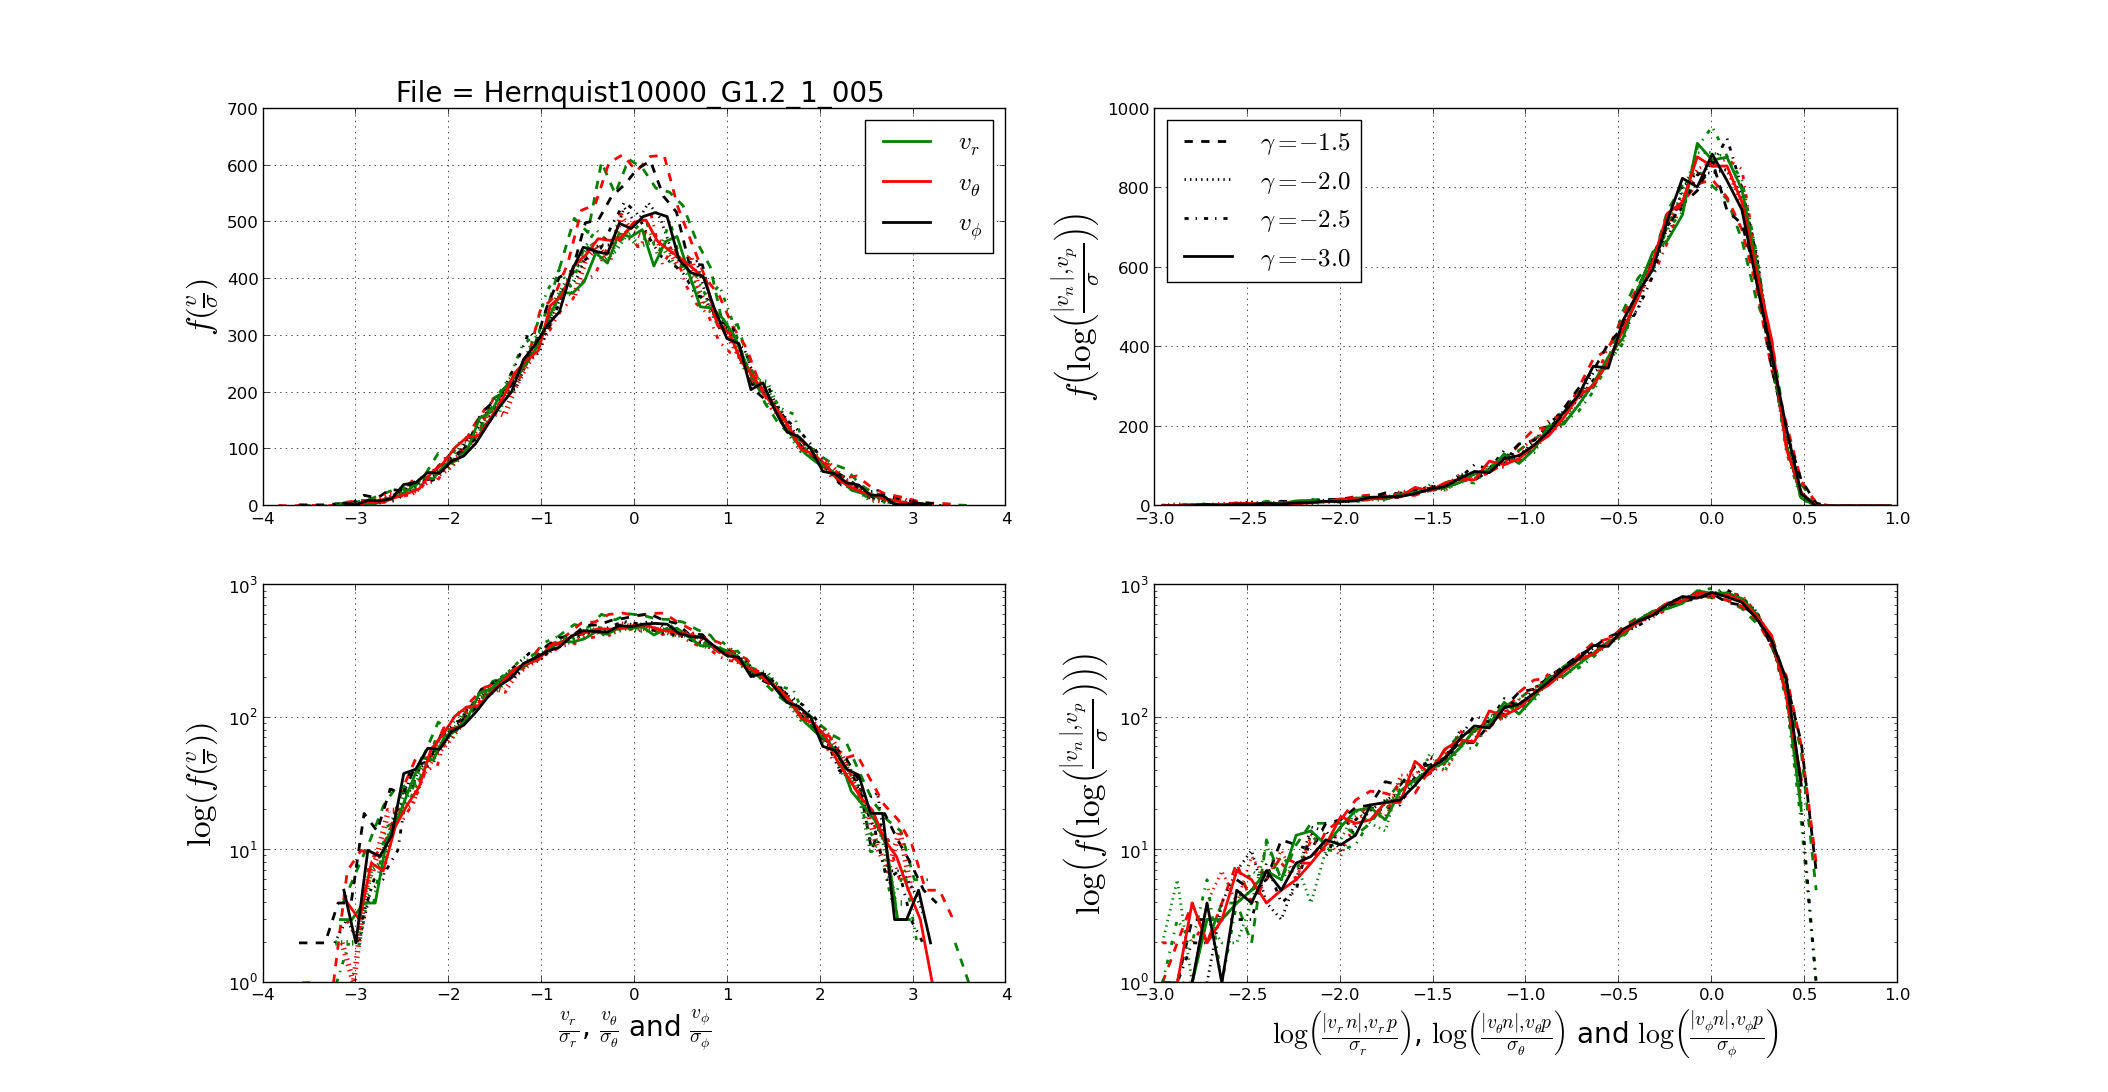
\includegraphics[width=1.0\linewidth]{img/1.png}
\caption{$v_{r}$, $v_{\theta}$ and $v_{\phi}$ divided by $\sigma_{r}$, $\sigma_{\theta}$ and $\sigma_{\phi}$ respectively, for 4 different radial bins. Shown in lin-lin, lin-log, log-lin and log-log}
\label{fig:test}
\end{figure}

\begin{figure}
\centering
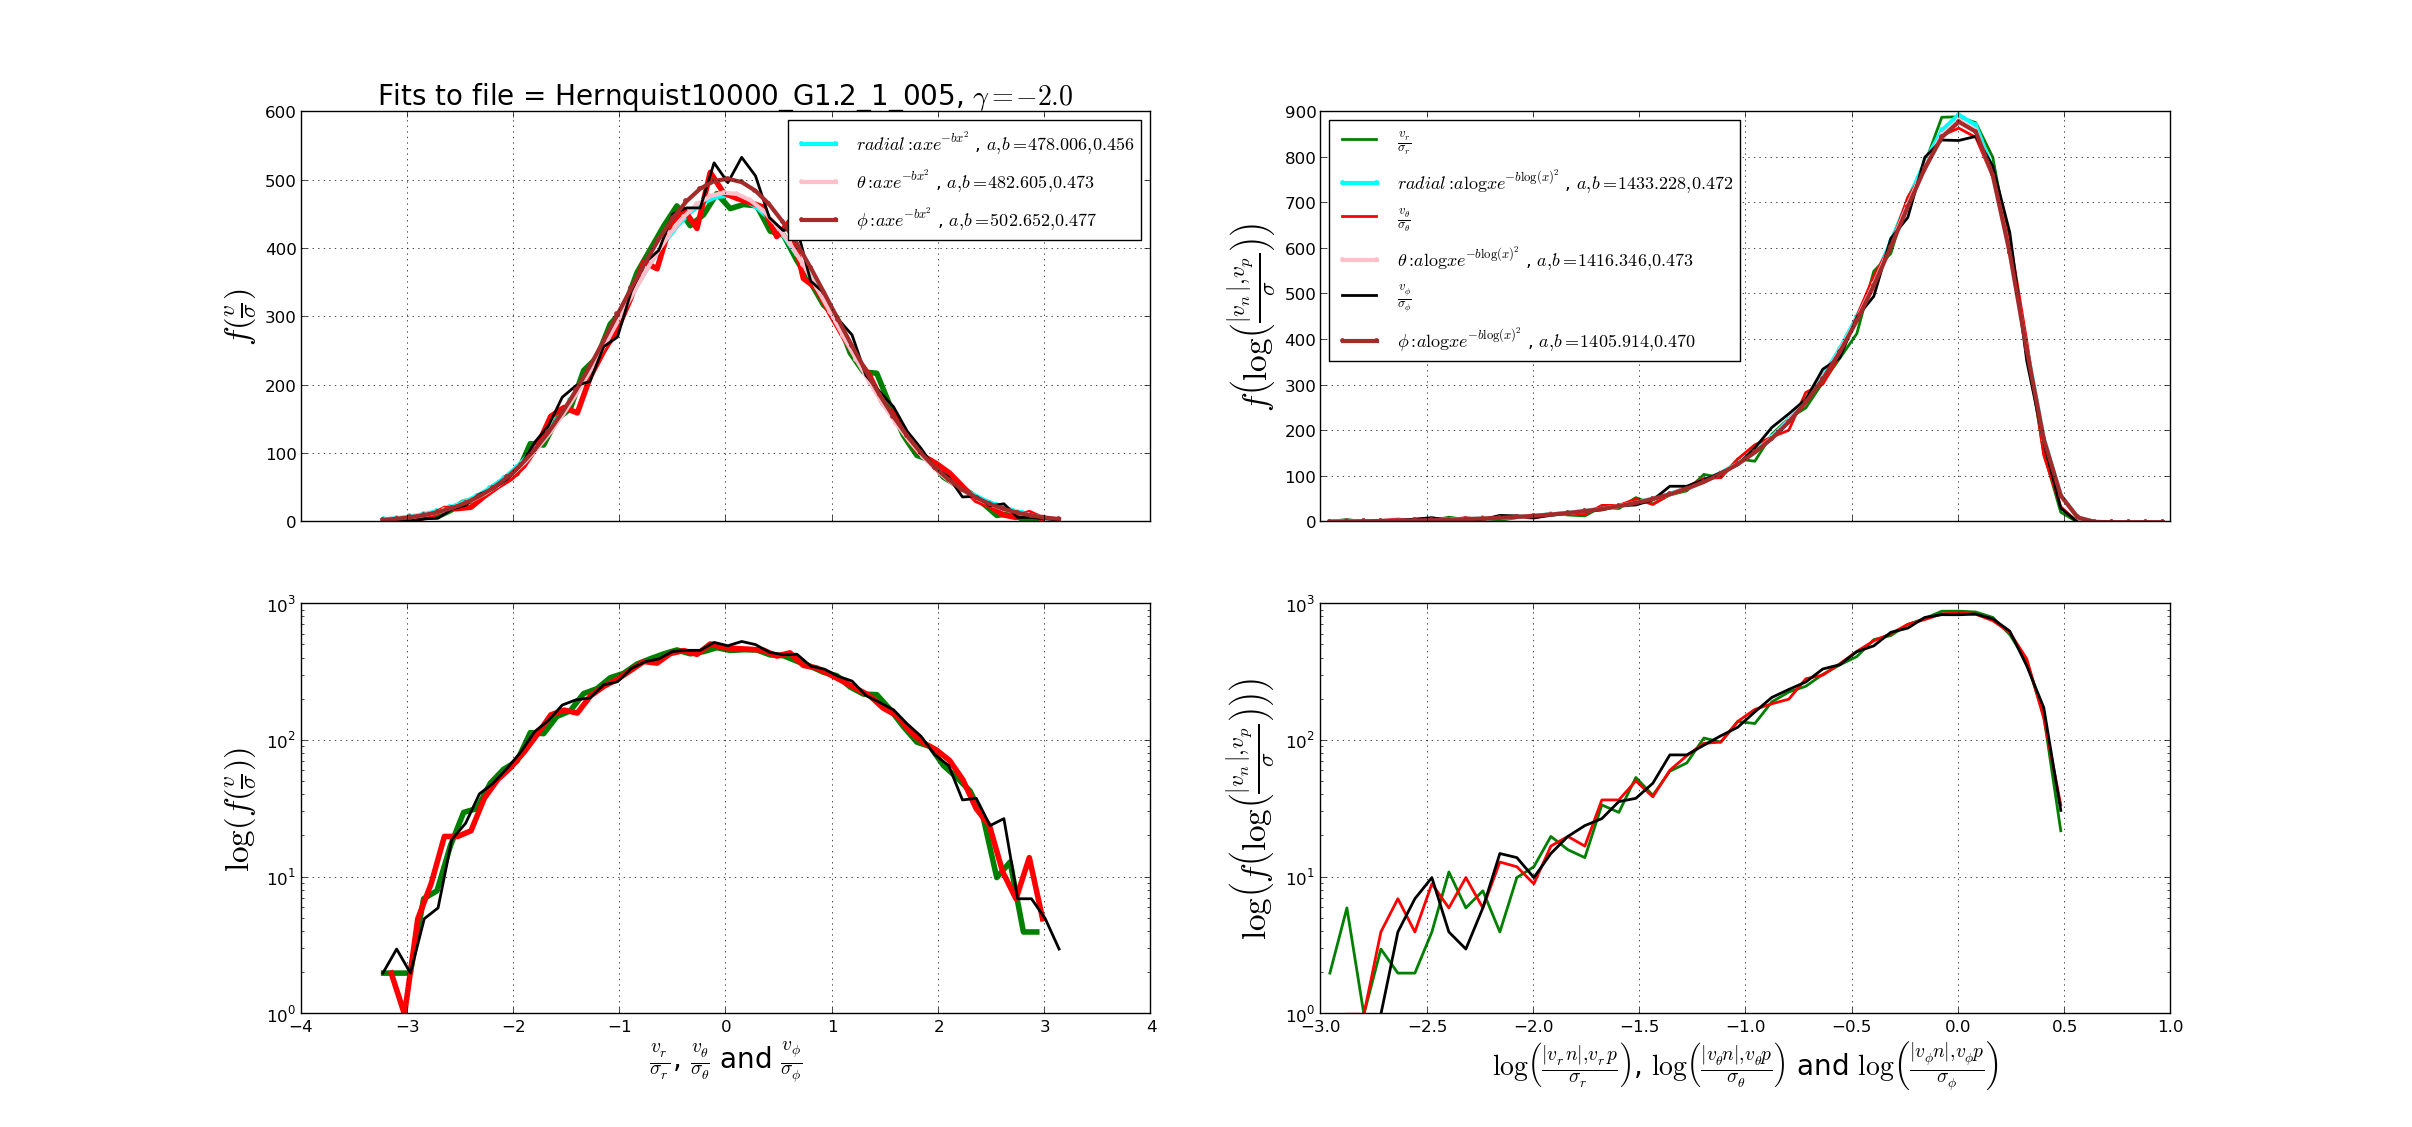
\includegraphics[width=1.0\linewidth]{img/vr_vtheta_vphi_fit.png}
\caption{$v_{r}$, $v_{\theta}$ and $v_{\phi}$ together with Gaussian and Tsallis fit.}
\label{fig:test}
\end{figure}

\begin{figure}
\centering
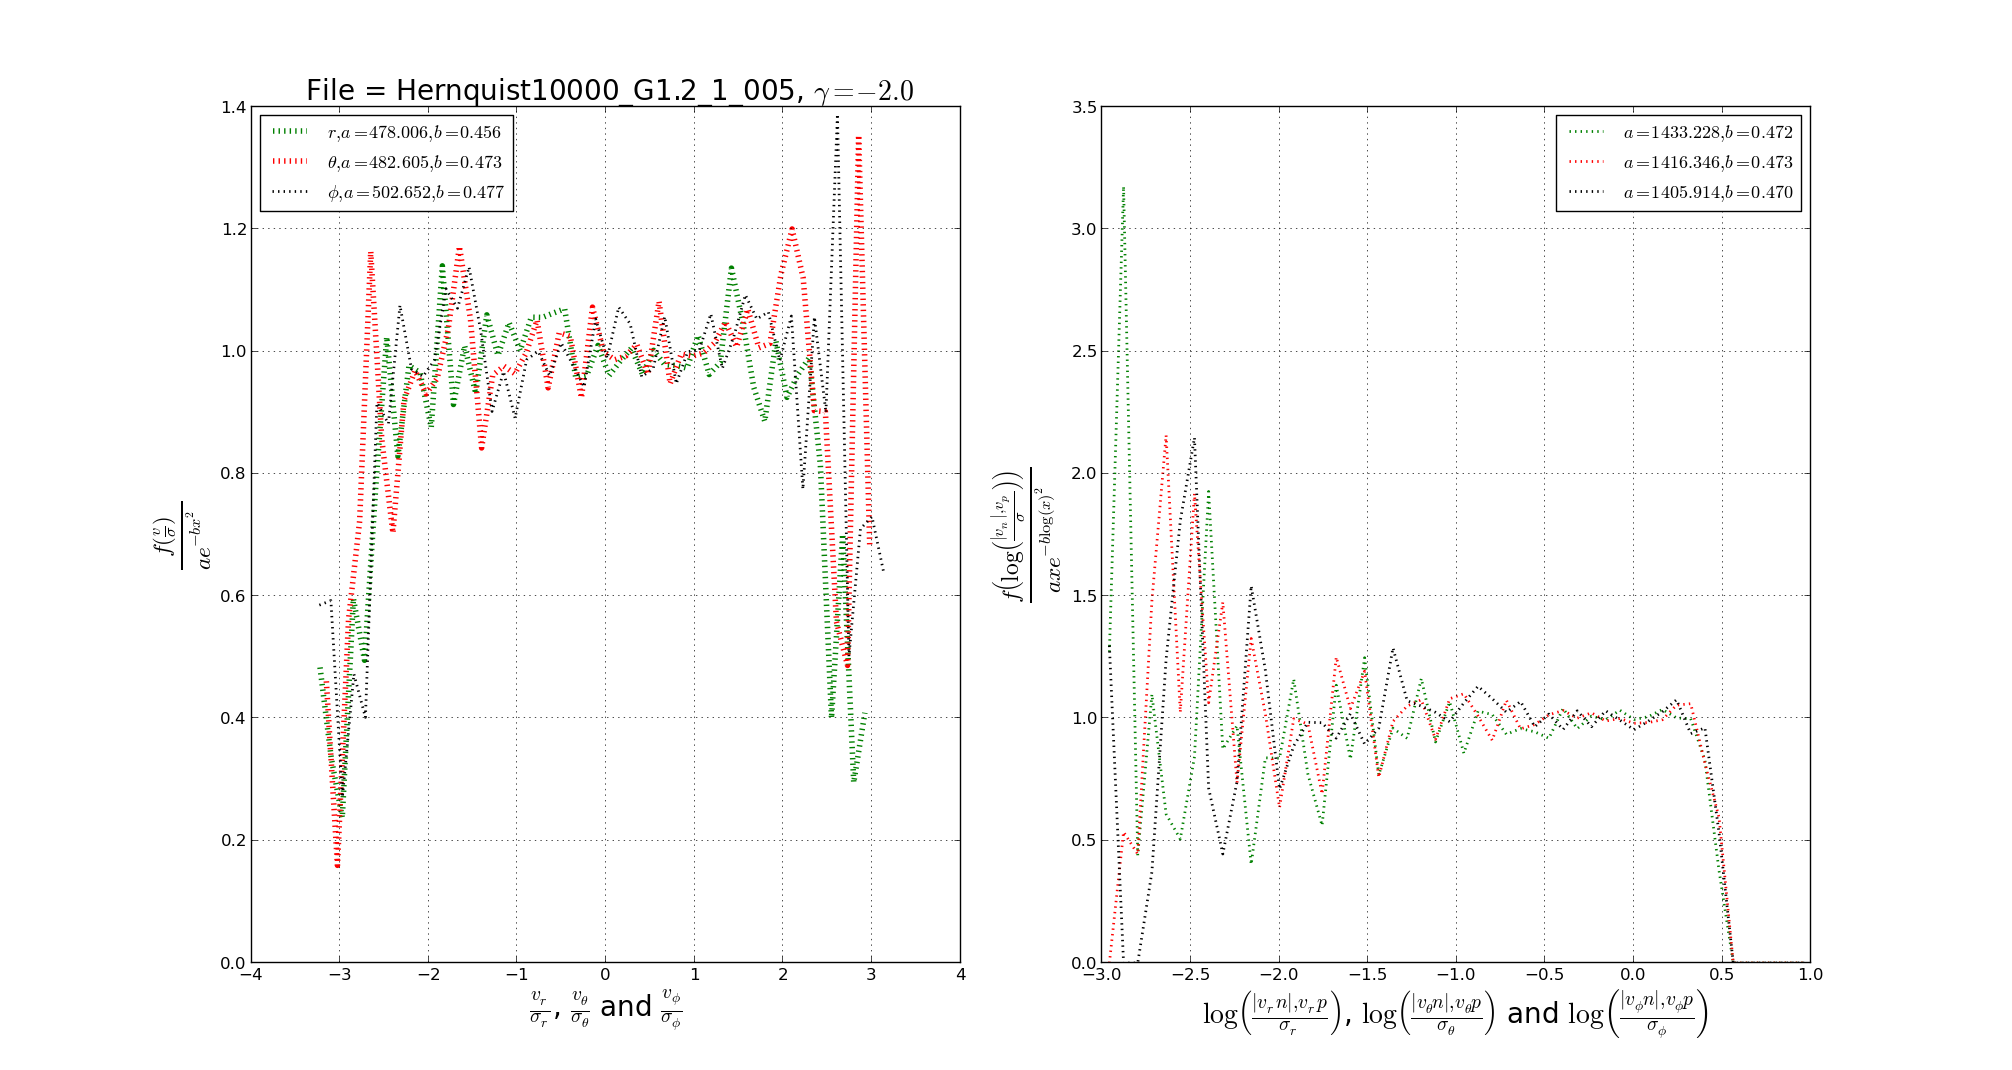
\includegraphics[width=1.0\linewidth]{img/func_guess_vr_vtheta_vphi.png}
\caption{$v_{r}$, $v_{\theta}$ and $v_{\phi}$ divided by Gaussian function.}
\label{fig:test}
\end{figure}

\newpage
\subsection{Line-of-sight overdensities}
Starting with an end-product from a G-perturbation simulation, which is no longer perfectly spherical and therefore more closely resembles a cosmological DM halo, a plot of radial velocity, $v_r$ vs. radius, r (for a 3D simulation file) is compared to the corresponding plot of velocity along the x-direction, $v_x$ (taken to be the line-of-sight, LOS) vs the projected radius, R (given by $R = \sqrt{y^2+z^2}$).
It is possible to simulate 3D structures, but in reality it is only possible to observe the LOS-velocity, $v_{LOS}$ here defined to be $v_x$. R is the projected radius onto LOS and r is here the 3D radius vector from the simulation.
An interesting question to investigate is: How does overdensities in 3D look in this corresponding 2D representation ($v_x$ vs $R$)?

%\begin{figure}
%\centering
%\includegraphics[width=1.0\linewidth]{img/endproduct_gamma.png}
%\caption{}
%\label{fig:test}
%\end{figure}

%\begin{figure}
%\centering
%\includegraphics[width=1.0\linewidth]{img/endproduct_kappa.png}
%\caption{}
%\label{fig:test}
%\end{figure}

%\begin{figure}
%\centering
%\includegraphics[width=1.0\linewidth]{img/endproduct_beta.png}
%\caption{}
%\label{fig:test}
%\end{figure}

%\begin{figure}
%\centering
%\includegraphics[width=1.0\linewidth]{img/endproduct_sigmas.png}
%\caption{}
%\label{fig:test}
%\end{figure}

%\begin{figure}
%\centering
%\includegraphics[width=1.0\linewidth]{img/LOS_gammaminus1_5.png}
%\caption{For the file Hernquist10000\_G1.0\_10\_009 we here see a comparison of the radial velocity as function of radius (left panel)
%to the LOS-velocity vs the projected radius. It is shown for a radial bin containing $10^4$ particles, centered around the radius where $\gamma = -1.5$}
%\label{fig:test}
%\end{figure}

%\begin{figure}
%\centering
%\includegraphics[width=1.0\linewidth]{img/LOS_gammaminus2_0.png}
%\caption{For the file Hernquist10000$\_$G1.0$\_$10$\_$009 we here see a comparison of the radial velocity as function of radius (left panel)
%to the LOS-velocity vs the projected radius. It is shown for a radial bin containing $10^4$ particles, centered around the radius where $\gamma = -2.0$}
%\label{fig:test}
%\end{figure}

\begin{figure}
\centering
\includegraphics[width=1.0\linewidth]{img/LOS.png}
\caption{For the file Hernquist10000$\_$G1.0$\_$10$\_$009 containing $10^6$ particles we here see a comparison of the radial velocity as function of radius (left panel) to the LOS-velocity vs the projected radius for the G-perturbation simulation. The left panel showing the radial velocity clearly portrays the presence of substructure which is washed out in the corresponding line-of-sight plot in the right plot. This point makes it clear that numerical simulations can provide a full picture absent when performing observations naturally restricted to the line of sight. The radial velocity plot has 5 distinct filaments, one for each of the perturbations. The filament furthest to the right corresponds to the first time particles escapes the structure.}
\label{fig:test}
\end{figure}

The biggest difference between the $r, v_r$-graph and the $R, v_x$-graph is the amount of information lost when going from 3D quantities to line-of-sight quantities.
Notice in particular the high degree of substructure in the $r, v_r$-graph;
we see 5 arms corresponding to each variation of G, which is in a way frozen into the phase-space volume. When G is increased, the radial velocity grows rapidly for larger radii, and when G is decreased, the radial velocity falls off just as rapid. 

\begin{figure}
\centering
\includegraphics[width=1.0\linewidth]{img/LOS_logr.png}
\caption{For the file Hernquist10000$\_$G1.0$\_$10$\_$009 containing $10^6$ particles we here see a comparison of the radial velocity as function of logarithmic radius (left panel) to the LOS-velocity vs the logarithmic projected radius. This gives a great resolution of the center.}
\label{fig:test}
\end{figure}

\begin{figure}
\centering
\includegraphics[width=1.0\linewidth]{img/LOS_radius50_N1000.png}
\caption{For the file Hernquist10000$\_$G1.0$\_$10$\_$009 we here see a comparison of the radial velocity as function of radius and logarithmic radius (left panel) to the LOS-velocity vs the projected radius and logarithmic projected radius. A thousand particles have been picked out for this analysis and the structure is cut off at radius = 50.
Looking at the top left subplot, basically the same number of particles seems to be present both above and below the zero-line at inner and middle-regions. at $r>40$ positive radial velocities starts to dominate over negative ones indicating a small particle flow away from the structure at large radii. This is expected as outer particles are less bound and might not have had sufficient time to reach equilibrium.}
\label{fig:test}
\end{figure}

This figure shows the inner part (up to radius 50) of the phase-space volume for particles in the file Hernquist10000$\_$G1.0$\_$10$\_$009.
If we pay close attention to the zero-line on the y-axis, in general we find as many particles over as under this line in the most central part up until about radius 20.
The central part is thus symmetric around the zero line. At higher radii there tend to be more particles with positive radial velocities which are the ones that has escaped the structure and will continue heading outwards forever.
This means that the central phase-space volume of particles are in equilibrium, but the outer part is not. The outer particles below the horizontal zero-line are heading towards the central phase-space volume again. This is particles experiencing a bit of infall.  We can thus track the particles which are no longer bound.

\newpage
\subsection{The bumpy road to universalities}

\begin{figure}
\centering
\includegraphics[width=1.0\linewidth]{img/BC4C5C6D1D2_sigmar2_vr_logr_panel.png}
\caption{The final products for the simulations \emph{B, $C_4$, $C_5$, $C_6$, $D_1$ and $D_2$}. Here $\sigma_r^2$ vs. logarithmic radius and radial velocity vs the logarithmic radius is shown. $N = 10^5$ particles are used for this analysis and the structure is cut off at radius = 10000.}
\label{fig:test}
\end{figure}

From the top panel of figure 51 there appear to be some overall trends to $\sigma_r^2$:
in the inner part, Sim B clearly has the largest $\sigma_r^2$, which then becomes smaller than the other simulations $\sigma_r^2$ in the outer part. 
From the bottom panel of figure 51 it is seen that on average there is the same amount of radial velocities above and below the zero line at inner and middle regions. This indicates the structures are in equilibria here and their particles are gravitationally bound. The outer region has an increase in radial velocities due to a few unbound particles which dominate the picture here. These have later been removed from the structures which then become flattened in this type of plot even for outer regions.

\begin{figure}
\centering
\includegraphics[width=1.0\linewidth]{img/BC4C5C6D1D2_gamma.png}
\caption{IC and final products for the simulations \emph{B, $C_4$, $C_5$, $C_6$, $D_1$ and $D_2$}.
The final products show universal trends: there seem to be three distinct local minima and similarly three distinct local maxima to the $\gamma$ profiles at the outer volume (where $\log r > 1 $) of the various structures. For $D_1$ and $D_2$ the extrema almost overlap, which is also the case for $C_4$, $C_5$ and $C_6$. B has unique positions of extrema.}
\label{fig:test}
\end{figure}

\begin{figure}
\centering
\includegraphics[width=1.0\linewidth]{img/C4C5C6D1D2_gamma_d3.png}
\caption{Final products for the simulations \emph{$C_4$, $C_5$, $C_6$, $D_1$ and $D_2$}.
Here the individual $\gamma$ profiles are shown vs. $\log ( \frac{r}{d_3})$, where $d_3$ are the $\gamma$-value of each profile at its third local minima. }
\label{fig:test}
\end{figure}

\begin{figure}
\centering
\includegraphics[width=1.0\linewidth]{img/D1D2_gamma_logr_panel.png}
\caption{Time evolution of $\gamma$-profile for the final states of the unstable structure $D_1$ (left panel) and the final states of the stable structure $D_2$ (right panel) from sim. I. From the top and downwards the number of radial bins is 20, 50, 100 and 200 respectively. The final states are 48$\_$093
and 49$\_$093 for both structures. From plots like these it is concluded that the optimum number of radial bins for structures with $N = 10^5$ particles is 20 and that the optimum number of radial bins for structures with $N = 10^6$ particles is 50.}
\label{fig:test}
\end{figure}

\begin{figure}
\centering
\includegraphics[width=1.0\linewidth]{img/BC4C5C6D1D2_r_logr_ur_mean_timemax_4600.png}
\caption{Final products for the simulations \emph{B, $C_4$, $C_5$, $C_6$, $D_1$ and $D_2$}.
Here the radial velocities divided by the radial velocity dispersions are shown vs. r and $\log r $, for both 50 and 20 radial bins. }
\label{fig:test}
\end{figure}

\begin{figure}
\centering
\includegraphics[width=1.0\linewidth]{img/BC4C5C6D1D2_logr_ur_mean_timemax_4600_zoom.png}
\caption{Zoom in on previous figure. Due to Poisson noise, the regions logr < -1 and logr > 2 can not be trusted. The vertical axis showing $u_r$ has also been narrowed down to a smaller range for more clarity.}
\label{fig:test}
\end{figure}
\newpage
\section{Functional analysis}
\textbf{Functional analysis of the $\beta$ and $\gamma$ functions are performed graphically together with a presentation of the restriction $\beta < -\frac{\gamma}{2}$ which has to be met in order to obtain stable structures (An $\&$ Evans 2006).} \\ 

A structure which lie in the region where $\beta > -\frac{\gamma}{2}$ might be created, but as soon as the time integration begins the structure will no longer be stable. This unstable region is shown in figure 19 as a pink region in the upper right corners of each subplot. It has been found to be unstable by An $\&$ Evans in 2006;i.e. for a cusped density profile which goes as $r^{\gamma}$ near the center, the limiting value of the anisotropy parameter $\beta$ cannot be greater than $-\frac{\gamma}{2}$ at the center. It follows from the non-negativity of the phase-space density. By tuning the two parameters $r_a$ (anisotropy radius) and $r_s$ (scale radius) it is possible to approach the unstable region without ever crossing into it. This knowledge is helpful when choosing how to set up the initial structure; If one wishes to create a stable structure close to or far away from the unstable region one simply has to make the corresponding choices for these two parameters. We learn from figure 19 that a small value of $r_a$, a large value of $r_s$ can bring our structure closer to the unstable region. Notice how these effects are unaffected by our choice of $\rho_0$ as it is a constant that will not affect the differentiation performed when computing the $\gamma$ array. But in practical purposes it is best to make some compromise to avoid too large of a computational cost (longer simulation time). Also, there is no guarantee that a structure outside the unstable region is stable. This has to be checked. In fact the contrary might be true as well; It might be possible to create a stable structure that crosses into the pink region and out again, since the An $\&$ Evans paper from 2006 only concludes this instability based on a smooth $\gamma$-profile. 
\begin{figure}[!htbp]
\centering
\includegraphics[width=1.0\linewidth]{img/beta_gamma_functions.png}
\caption{Analysis of the $\beta$ and $\gamma$ functional expressions for different choices of scale radius and anisotropy radius. The $\rho_0$ normalization parameter is kept fixed at $\rho_0 = \frac{1}{2 \pi}$. Plotted together with the unstable region where $\beta > -\frac{\gamma}{2}$. This figure gives a qualititive idea of the kind of structures that might fall into the stable category.}
\label{fig:test}
\end{figure}
\begin{figure}[!htbp]
\centering
\includegraphics[width=1.0\linewidth]{img/A_IC_xy_xz.png}
\caption{2D view of IC for structure A. we first see the particles y-positions vs. their x-positions and then their z-positions vs. their x-positions. The halo is cut off at a radius of $R_{lim}=32$.}
\label{fig:test}
\end{figure}
For all structures, the characteristic radius is $r_s = 1$, and the normalization constant $\rho_0 $ has been chosen so that the total mass inside $r = 13r_s$ is 1. This ensures that the dynamical time mentioned in the previous section , for particles inside $r = 13r_s$ is smaller than 100 time units (which is the duration of all simulations performed). For the Osipkov-Merritt model, we have seen in the previous section that the $\beta$ profile is 
\begin{equation}
\beta = \frac{r^2}{r^2 + r_a^2}  
\end{equation}
The anisotropy radius $r_a$ is varied from $1.2 r_s$ to $ 0.2 r_s $. When $r_a$ exceeds $r_s$ instabilities can be avoided. It is shown (Kazantzidis, Stelios)  that $r_a \geq 1.33r_s$ will ensure stability. In the setup the particle number is varied from $ 10^4 $ to $ 10^6 $.
\newpage
\section{Brief overview and description of analysis codes}

\subsection{VDFs}
The analysis is done with three separate programs which I have written in the Python programming language. Amongst other things they agree with cosmological simulations about virial radius which tend to be $r_{vir}=10r_{-2}$, with $r_{-2} = \frac{r_s}{2}$ (for a Hernquist profile). For a NFW profile, $r_s=r_{-2}$. To see the programs, look under appendices D, E and F, where there is also a short introduction to each program. Comment lines are included into the code, to clarify each step taken. In this section I will simply attempt to highlight the most prominent features of each of these codes. For the first code, 'Read.py', the central part is the following for-loop which we shall now investigate further: \\ 

\begin{pythonstyle}
\begin{lstlisting}[language=Python]
# Divide the structure into logarithmic radial bins
for i in range(0, int(nr_binning_bins)):      # loop over the number of bins 
    min_R_bin_i = binning_arr_lin_log10[i]    # start of bin 
    max_R_bin_i = binning_arr_lin_log10[i+1]  # end of bin 
    posR_par_inside_bin_i = np.where((R>min_R_bin_i) & (R<max_R_bin_i))[0] # position of particles inside a radial bin 
    # number of particles inside a radial bin:    
    nr_par_inside_bin_i   = len(posR_par_inside_bin_i)                     
    # Volume of cluster: 
    Volume_cl = (4./3.)*np.pi*(max_R_bin_i**3 - min_R_bin_i**3) 
    den_cl = nr_par_inside_bin_i/Volume_cl # number density 
    rho_cl = m*den_cl                      # density (m is the mass of each particle, m = M/N = 1/N)
    # save to lists 
    density_arr.append(den_cl) 
    Volume_arr.append(Volume_cl) 
Invers_Volume_arr = np.log10(np.divide(np.ones(len(Volume_arr)),Volume_arr)) 
\end{lstlisting}
\end{pythonstyle}

After cutting the cluster structure up into logarithmic linear radial bins, each bin contains a certain number of particles whose various physical quantities is then averaged,e.g. the number density given by number of particles in each bin divided by the volume of this spherical shell. The number of particles for a certain bin, i,  is found by taking the length of the array containing all particles inside  bin\_i. The volume of a spherical shell in general is just the volume of the remainder of the whole sphere´s volume after subtracting the volume of the inside sphere (with radius equal to the start value of the bin radius). This is then used in the line above which writes  \\
\begin{pythonstyle}
\begin{lstlisting}[language=Python]
Volume_cl = (4./3.)*np.pi*(max_R_bin_i**3 - min_R_bin_i**3)
\end{lstlisting}
\end{pythonstyle}
So now the number density is ready to be plotted, and can be fitted with a Hernquist density profile. (for comparison I also fitted with a NFW-profile). In the second analysis code, 'Sigma.py', the most central aspect is firstly to find the velocity dispersions and secondly to compute the $ \beta$, $ \kappa$ and $ \gamma$ variables. Let us first see how the velocity dispersions are found. Basically it is an expansion of the previous for-loop used to find the density. \\ \\
\begin{pythonstyle}
\begin{lstlisting}[language=Python]
for i in range(nr_binning_bins):            # loop over the number of bins  
    min_R_bin_i = binning_arr_lin_log10[i]    # start of bin 
    max_R_bin_i = binning_arr_lin_log10[i+1]  # end of bin 
    posR_par_inside_bin_i = np.where((R_hob_par>min_R_bin_i) & (R_hob_par<max_R_bin_i)) # Particle positions
    nr_par_inside_bin_i = len(posR_par_inside_bin_i[0])   # number of particles inside a radial bin 
    if nr_par_inside_bin_i == 0: 
        continue 
    v2_inside_bin_i = v2[posR_par_inside_bin_i] 
    sigma2_inside_bin_i = (1./(nr_par_inside_bin_i+1.))*np.sum(v2_inside_bin_i) 
    sigma2_arr.append(sigma2_inside_bin_i) # sigma2 total 
    bin_radius_arr.append((max_R_bin_i + min_R_bin_i)/2) 
    # sigmarad2 radial 
    vrad2_inside_bin_i = v_r[posR_par_inside_bin_i]**2 
    sigmarad2_inside_bin_i = (1./(nr_par_inside_bin_i+1.))*np.sum(vrad2_inside_bin_i) 
    sigmarad2_arr.append(sigmarad2_inside_bin_i) 
    Volume_cl = (4./3.)*np.pi*(max_R_bin_i**3 - min_R_bin_i**3) # cluster volume
    den_cl = nr_par_inside_bin_i/Volume_cl # number density 
    rho_cl = m*den_cl     # density (m is the mass of each particle, m = M/N = 1/N)
    density_arr.append(den_cl)   # save array
    Volume_arr.append(Volume_cl) # save array 
sigma2_arr     = np.array(sigma2_arr)      # square of total velocity dispersion 
sigmarad2_arr  = np.array(sigmarad2_arr) 
bin_radius_arr = np.array(bin_radius_arr) 
\end{lstlisting}
\end{pythonstyle}

Notice the way the total velocity dispersion, $\sigma^2$, is found by dividing the sum of the square of the velocities by the number of particles. Normally the sum would contain the difference of the velocities and the mean velocity, squared, but the mean velocity is already accounted for by defining new velocities, in order to make this loop simpler. The radial velocity dispersion , sigmarad2, is found in an analogous way, by dividing the sum of the square of the radial velocities by the number of particles. The tangential velocity dispersion is then just a question of subtracting the radial from the total velocity dispersion, and we have all three. They can now be used to compute the $ \beta$, $ \kappa$ and $ \gamma$ variables: \\

\begin{pythonstyle}
\begin{lstlisting}[language=Python]
# kappa 
for  i in range(len(sigma2_arr)): 
    if i == 0 or i == len(sigma2_arr)-1: 
        kappa_arr.append(np.nan) 
        continue 
    dlogr         = np.log10(bin_radius_arr[i+1]) - np.log10(bin_radius_arr[i-1]) 
    dlogsigmarad2 = np.log10(sigmarad2_arr[i+1])  - np.log10(sigmarad2_arr[i-1]) 
    kappa_arr.append(dlogsigmarad2/dlogr) 
# gamma 
for  i in range(len(density_arr)): 
    if i == 0 or i == len(sigma2_arr)-1: 
        gamma_arr.append(np.nan) 
        continue
    dlogr   = np.log10(bin_radius_arr[i+1]) - np.log10(bin_radius_arr[i-1])
    dlogrho = np.log10(density_arr[i+1]) - np.log10(density_arr[i-1])
    gamma_arr.append(dlogrho/dlogr)
# calculate sigmatheta 
sigmatheta2_arr = (sigma2_arr - sigmarad2_arr)/2. 
# calculate beta 
beta	_arr = 1. - sigmatheta2_arr/sigmarad2_arr 
\end{lstlisting}
\end{pythonstyle}

The strategy employed here to find $ \kappa$ is first finding $d \log r$, then $d \log \sigma_{rad}^2$ and their ratio, $\frac{d \log \sigma_{rad}^2}{d \log r}$. Very similar for $\gamma$, $d \log r$ is found, then $d \log \rho$, and then taking the ratio between the two, $\frac{d \log \rho}{d \log r}$. Now for $\beta$, it´s simply $ \beta \equiv 1 - \frac{\sigma_{\theta}^2}{\sigma_{rad}^2}$. This is done for all datasets, plotted, and saved as text files to be used in the following. Third and final analysis program, 'gamma\_kappa\_beta.py' now takes the text files from previous code, and overplots them. This shows clear indication of a preférred structure in ($\beta$,$\gamma$,$\kappa$)-space, see conclusion in next section.

\begin{figure}
\centering
\begin{subfigure}{.5\textwidth}
  \centering
  \includegraphics[width=1.0\linewidth]{img/Read_ics_1.png}
  \caption{High resolution}
  \label{fig:sub1}
\end{subfigure}%
\begin{subfigure}{.5\textwidth}
  \centering
  \includegraphics[width=1.0\linewidth]{img/Read_ICS_10MPC_1.png}
  \caption{Low resolution}
  \label{fig:sub2}
\end{subfigure}
\caption{Image of the 10 Megaparsec structure from the Gadget-2 simulation with G-perturbations. The most luminous clumps in the structure are galaxy cluster halos of dark matter.}
\label{fig:test}
\end{figure}

\begin{figure}
\centering
\includegraphics[width=1.0\linewidth]{img/Read_ics_2.png}
\caption{From the previous high resolution image of the 10 Mpc structure, 
the largest galaxy cluster halo of dark matter has been cut out to produce this image.}
\label{fig:test}
\end{figure}

\begin{figure}
\centering
\includegraphics[width=1.0\linewidth]{img/Read_OG_IC_2.png}
\caption{Initial plot of G-perturbations with $ \beta = 0$ for a Hernquist structure (0G00\_IC\_000.hdf5).}
\label{fig:test}
\end{figure}

\begin{figure}
\centering
\includegraphics[width=1.0\linewidth]{img/Read_OG_Final_2.png}
\caption{Final plots of G-perturbations with $ \beta = 0$ for a Hernquist structure (0G20\_Final\_000.hdf5). Notice the structure has expanded significantly with respect to the initial structure.}
\label{fig:test}
\end{figure}

\begin{figure}
\centering
\begin{subfigure}{.5\textwidth}
  \centering
  \includegraphics[width=1.0\linewidth]{img/Read_OMGOO_IC_1.png}
  \caption{The whole structure}
  \label{fig:sub1}
\end{subfigure}%
\begin{subfigure}{.5\textwidth}
  \centering
  \includegraphics[width=1.0\linewidth]{img/Read_OMGOO_IC_2.png}
  \caption{Zoom-in on cluster}
  \label{fig:sub2}
\end{subfigure}
\caption{Initial plots of Osipkov-Merritt structure before G-perturbations.}
\label{fig:test}
\end{figure}

\begin{figure}
\centering
\begin{subfigure}{.5\textwidth}
  \centering
  \includegraphics[width=1.0\linewidth]{img/Read_OMGOO_Final_1.png}
  \caption{The whole structure}
  \label{fig:sub1}
\end{subfigure}%
\begin{subfigure}{.5\textwidth}
  \centering
  \includegraphics[width=1.0\linewidth]{img/Read_OMGOO_Final_2.png}
  \caption{Zoom-in on cluster}
  \label{fig:sub2}
\end{subfigure}
\caption{Final plots of Osipkov-Merritt structure after G-perturbations. Again we see how the structure has expanded significantly. }
\label{fig:test}
\end{figure}

\begin{figure}
\centering
\begin{subfigure}{.5\textwidth}
  \centering
  \includegraphics[width=1.0\linewidth]{img/Read_OMGOO_IC_3.png}
  \caption{Initially the central potential is close \\ to the value of -1}
  \label{fig:sub1}
\end{subfigure}%
\begin{subfigure}{.5\textwidth}
  \centering
  \includegraphics[width=1.0\linewidth]{img/Read_OMGOO_Final_3.png}
  \caption{Finally the central potential is seen in the semi-logarithmic plot to have a value of about \\ -0.25. }
  \label{fig:sub2}
\end{subfigure}
\caption{Gravitational potential for Osipkov-Merritt data. First subplot is $\Phi$ shown versus radius, whereas the second plot is against logarithmic radius, to resolve the central region in greater detail. The lessening of the central potential is to be expected since we already saw in a previous plot how the structure expands and therefore feels a numerically smaller central gravitational potential.}
\label{fig:test}
\end{figure}

\begin{figure}
\centering
\begin{subfigure}{.5\textwidth}
  \centering
  \includegraphics[width=1.0\linewidth]{img/Read_OMGOO_IC_5.png}
  \caption{Initially all velocities are almost identical}
  \label{fig:sub1}
\end{subfigure}%
\begin{subfigure}{.5\textwidth}
  \centering
  \includegraphics[width=1.0\linewidth]{img/Read_OMGOO_Final_5.png}
  \caption{The final picture is quite different. Now the velocities are completely different along each axis.}
  \label{fig:sub2}
\end{subfigure}
\caption{Velocities of particles , inside cluster of Osipkov-Merritt data, with respect to the clusters own velocity. From left to right we see particle velocities along the x, y and z-axis, all plotted as a function of the x-axis.}
\label{fig:test}
\end{figure}

\newpage
\begin{figure}[h!]
	\centering
		\includegraphics[width=1.0\linewidth]{img/Attractor_fig1.png}
		{\medskip\caption{\textsl{Now that the $\gamma$ ,$\kappa $ and $\beta$- profiles have been determined, the attractor in $(\gamma,\kappa,\beta)$-space can be created for all datasets. Notice how the upper right corner is always completely empty in the ($\beta$,$\gamma$)-plot. This is due to the constraint put by the inequality $ \beta < -\frac{\gamma}{2}$ (An \& Evans 2006).
\label{fig:Rv}}}}
\end{figure} 

\begin{figure}[h!]
	\centering
		\includegraphics[width=1.0\linewidth]{img/Attractor_fig2.png}
		{\medskip\caption{\textsl{In the previous figure the IC and Final products had been overplotted. Here they can be seen independently.
\label{fig:Rv}}}}
\end{figure} 

\begin{figure}[h!]
	\centering
		\includegraphics[width=1.0\linewidth]{img/Attractor_fig3.png}
		{\medskip\caption{\textsl{It is more clear to identify an attractor when $\gamma + \kappa$ is plotted vs. $\beta$, instead of splitting it up into two separate plots.
\label{fig:Rv}}}}
\end{figure} 

\begin{figure}[h!]
	\centering
		\includegraphics[width=1.0\linewidth]{img/Attractor_3D.png}
		{\medskip\caption{\textsl{3D view of attractor.
\label{fig:Rv}}}}
\end{figure} 

\begin{figure}[h!]
	\centering
		\includegraphics[width=1.0\linewidth]{img/C1C2C3_beta_gamma_kappa.png}
		{\medskip\caption{\textsl{$\gamma$ vs. $\beta$ and $\kappa$ vs. $\beta$ for 50 and 20 radial bins is here shown for the ICs of sims. $C_1$, $C_2$ and $C_3$ which each hold a total number of $N = 10^4$ particles. $R_{limit} = 5 \cdot 10^2$.
50 bins introduces random scatter due to bad resolution and is not physical.
\label{fig:Rv}}}}
\end{figure} 

\begin{figure}[h!]
	\centering
		\includegraphics[width=1.0\linewidth]{img/C4C5C6_beta_gamma_kappa.png}
		{\medskip\caption{\textsl{$\gamma$ vs. $\beta$ and $\kappa$ vs. $\beta$ for 50 and 20 radial bins is here shown for the IC´s of SIMS $C_4$, $C_5$ and $C_6$ which each hold a total number of $N = 10^5$ particles. $R_{limit} = 5 \cdot 10^2$. 50 bins introduces random scatter due to bad resolution and is not physical.
\label{fig:Rv}}}}
\end{figure} 

\begin{figure}[h!]
	\centering
		\includegraphics[width=1.0\linewidth]{img/C4C5C6_beta_gamma_kappa_Final.png}
		{\medskip\caption{\textsl{$\gamma$ vs. $\beta$ and $\kappa$ vs. $\beta$ for 50 and 20 radial bins is here shown for the final products of sims. $C_4$, $C_5$ and $C_6$. $R_{limit} = 5 \cdot 10^2$. 50 bins introduces random scatter due to bad resolution and is not physical.
\label{fig:Rv}}}}
\end{figure} 

\begin{figure}[h!]
	\centering
		\includegraphics[width=1.0\linewidth]{img/D1D2_beta_gamma_kappa.png}
		{\medskip\caption{\textsl{$\gamma$ vs. $\beta$ and $\kappa$ vs. $\beta$ for 50 and 20 radial bins is here shown for the IC´s of sims. $D_1$ and $D_2$ which both hold a total number of $N = 10^5$ particles. $R_{limit} = 5 \cdot 10^2$. 50 bins introduces random scatter due to bad resolution and is not physical.
\label{fig:Rv}}}}
\end{figure} 

\begin{figure}[h!]
	\centering
		\includegraphics[width=1.0\linewidth]{img/D1D2_beta_gamma_kappa_Final.png}
		{\medskip\caption{\textsl{$\gamma$ vs. $\beta$ and $\kappa$ vs. $\beta$ for 50 and 20 radial bins is here shown for the final products of sims. $D_1$ and $D_2$. $R_{limit} = 5 \cdot 10^2$. 50 bins introduces random scatter due to bad resolution and is not physical.
\label{fig:Rv}}}}
\end{figure} 

\begin{figure}[h!]
	\centering
		\includegraphics[width=1.0\linewidth]{img/Attractor_fig4.png}
		{\medskip\caption{\textsl{$\gamma + \kappa$ vs. $\beta$ for IC and Final of SIMS B, 
$C_4$, $C_5$, $C_6$, $D_1$ and $D_2$. For the upper four subplots $R_{limit} = 5 \cdot 10^2$, and for the lower four subplots $R_{limit} = 10^4$. Shown for both 20 and 50 radial bins.
\label{fig:Rv}}}}
\end{figure} 

\begin{figure}[h!]
	\centering
		\includegraphics[width=1.0\linewidth]{img/Attractor_fig5.png}
		{\medskip\caption{\textsl{$\gamma + \kappa$ vs. $\beta$ for Final of SIMS B, 
$C_4$, $C_5$, $C_6$, $D_1$ and $D_2$ where all gravitationally unbound particles have been removed and the structures have had more time to equilibrate. $R_{limit} = 10^4$. 50 radial bins.
\label{fig:Rv}}}}
\end{figure} 

\subsection{Line-of-sight}

\subsection{Removing gravitationally unbound particles from structures}
To see the equilibrated structures from the final products more clearly, it is beneficial to remove the unbound particles which have escaped the gravitational potential of all the other particles. The total energy being positive is the condition which has to be met, in order to identify a free particle. This leads to the inequality $E_{tot} > 0 \rightarrow \Phi + \frac{1}{2}v^2 > 0$, where $\Phi$ is the gravitational potential of all the other particles and v is the speed of the particle under investigation. It is computed as $v = \sqrt{v_x^2+v_y^2+v_z^2}$. In practice this has been solved by writing all the bound particles (where $\Phi + \frac{1}{2}v^2 <= 0$) into a new HDF5 file, as deleting data inside a HDF5 file is rather complicated (commands such as HDF5DELETE does exist, and one could use this to destroy the link in the file to the data, after which the non-broken links can be saved in a new file, but that would be a messy solution). The new data is then inspected with the program HDFview to make sure the new file contain the right particles. The following table show the number of free and bound particles for final products of different SIMS:
\begin{table}[h]
\centering
\begin{tabular}{|c|c|c|c|c|c|c|}
\hline
         &     $B$    &    $C_4$  & $C_5$     & $C_6$     &  $D_1$    & $D_2$     \\ \hline
 File    & 199$\_$093 & 48$\_$093 & 48$\_$093 & 48$\_$093 & 49$\_$093 & 49$\_$093 \\ \hline
 N       &   $10^6$   &  $10^5$   & $10^5$    &  $10^5$   & $10^5$    & $10^5$  \\ \hline
 Bound   &   959845   &  58865    & 58917     &  58386    & 59340     & 66039  \\ \hline
 Unbound &   40155    &  41135    & 41083     &  41614    & 40660     & 33961  \\ \hline
\end{tabular}
\caption{From top to bottom: structure name, file number, total number of particles (N), number of bound particles and finally number of unbound particles. For all these files $G=1$.}
\end{table}
The bound particles from these simulations final products are thus saved into new files which are further simulated with GADGET-2 while G is kept equal to one for all these new files and they are all run for TimeMax = 2300. This result in the following files being created:
\begin{table}[h]
\centering
\begin{tabular}{|c|c|c|c|c|c|c|}
\hline
     &   $B$       &    $C_4$    &    $C_5$    &    $C_6$    &   $D_1$     &   $D_2$    \\ \hline
 N   &   959845    &    58865    &    58917    &    58386    &   59340     &   66039    \\ \hline
 Run No.       &   200       &     49      &     49      &      49     &     50      &     50     \\ \hline
\end{tabular}
\caption{From top to bottom: structure name, total number of particles N (Notice all gravitationally unbound particles have been removed), and finally number of the run is given. For all these files $G=1$.}
\end{table}

\begin{figure}
\centering
\includegraphics[width=1.0\linewidth]{img/B_final_vr_V_panel.png}
\caption{Final product of SIM B which have a total of $N = 10^6$ particles. Radial velocity vs. radius and logarithmic radius respectively. Gravitational potential vs. logarithmic radius.}
\label{fig:test}
\end{figure}

\begin{figure}
\centering
\includegraphics[width=1.0\linewidth]{img/B_rfp_vr_V_panel.png}
\caption{Final product of SIM B where all gravitationally unbound particles have been removed and the structures have had more time to equilibrate. Radial velocity vs. radius and logarithmic radius respectively. Gravitational potential vs. logarithmic radius. Notice how the outer regions now appear substantially different from the previous figure. There is a significant flattening of radial velocities in the scatterplots due to the removal of unbound particles as expected. The potential looks more or less the same apart from a slight contraction on the horizontal axis. This is natural as a removal of unbound particles that resided in the outer part of the structure lessens the gravitational pull outwards and the structure is therefore allowed to contract slightly more.}
\label{fig:test}
\end{figure}
\newpage

\begin{figure}
\centering
\includegraphics[width=1.0\linewidth]{img/BC4C5C6D1D2rfp_gamma_logr_panel.png}
\caption{The slope of the density profile, $\gamma$, vs. logarithmic radius for Final products of sims. B, $C_4$, $C_5$, $C_6$, $D_1$ and $D_2$ with structures containing all particles as well as same structures with only bound particles. 50 radial bins. $R_{limit} = 10^4$. Looking at the outer regions a clear effect is visible from the removal of gravitationally unbound particles: the final characteristic peak in the $\gamma$ profiles has dropped substantially.}
\label{fig:test}
\end{figure}

\begin{figure}
\centering
\includegraphics[width=1.0\linewidth]{img/BC4C5C6D1D2rfp_vr_logr.png}
\caption{Radial velocity vs. logarithmic radius for Final products of sims. B, $C_4$, $C_5$, $C_6$, $D_1$ and $D_2$ with structures containing all particles as well as same structures with only bound particles. 50 radial bins. $R_{limit} = 10^4$. The right panel shows zoom-ins of the left panel to investigate the mutual departures of the sims. around the middle region in more detail. Looking at the outer regions a clear effect is visible from the removal of gravitationally unbound particles: the increase in radial velocity has dropped substantially.
This might potentially make it possible to study the Jeans parameter attractor out to larger radii than previously.}
\label{fig:test}
\end{figure}
\newpage
\section{Background: Observational support to DM existence}
\textit{'Somewhere, something incredible is waiting to be known.'} \\
-- Carl Sagan \\ \\

DM was postulated by Jan Oort (1932) who studied orbital velocities of stars in the MW. Fritz Zwicky found there was missing mass (1933) when studying the orbital velocities of galaxies in the COMA cluster. The COMA cluster of galaxies (Abell 1656) is the home of more than one thousand galaxies. It is located inside the Coma Supercluster as a part of the Coma Berenices constellation. COMA is about $321 \cdot 10^6 $ light years away from earth. Horace W. Babcock studied galaxy rotation curves (1939) paving the road for Vera Rubin who postulated the existence of dark matter (1968) from galaxy rotation curves. Evidence for the existence of dark matter include gravitational lensing of distant astronomical objects by galaxy clusters such as the Bullet cluster and the COMA cluster (both micro-lensing and macro-lensing) and galaxy rotation curves which show velocities of galaxies inside clusters as a function of their distance to the cluster center. There is a discrepancy between the predicted theoretical curve (with only baryonic matter) and the observed curve which is much larger-valued for large distances to the cluster center. This is not possible if the only matter present is the visible that we observe, consider the virial theorem, $ K = \frac{1}{2} \cdot U $ where K and U are the kinetic and gravitational potential energy respectively. This is the simplified form of the theorem where the moment of inertia is neglected and thermal as well as magnetic energy is not considered. Another line of evidence for something extra is found in the CMB (more specifically, in the pattern of anisotropies in the CMB). Also we have the effects from Baryon Acoustic Oscillations (BAO); Basically it is periodic, regular fluctuations in the baryonic matter density which originated from the coupling (due to Thomson scattering) of free electrons and photons before recombination, that resulted in a distinct pattern of oscillations in the baryon and temperature power spectra. It acts as a standard ruler (of the order $490\cdot 10^6 $ lyr today) for length scales in cosmology, which can be estimated by astronomical surveys such as the Sloan Digital Sky Survey (SDSS). It is mainly used to research dark energy, but also requires constraining cosmological parameters such as the dark matter density. Newest Lyman $\alpha$ forest data exclude WDM models (Dwarf galaxies would be affected significantly). Finally should be mentioned the temperature distribution of hot gas in galaxies and galaxy clusters which point the way toward DM as well.
\newpage
\section{The GADGET-2 code}
\textit{In GADGET-2 the N-body simulations were run inside a non-cosmological Newtonian box, with only collisionless particles. This section provides some properties of the GADGET-2 code.} \\  

\centerline{\textbf{Leapfrog symplectic integrator.}} 
The system is integrated with a 2.nd order leapfrog integrator, which assures a symplectic behavior, that is, the total energy (Hamiltonian) is unchanged and the system is time-reversible. \\

\centerline{\textbf{simulation time and relaxation time.}} 
In general, Poisson solvers are used for N-body codes, both collisional and collisionless. Collisionless codes can model dark matter systems over times much shorter than $t_{relax}$. In real cosmological dark matter halos around galaxy clusters, the number of particles, N, could be much larger than the number of particles in these simulations. Because of this, $t_{relax}$ in the real structure could be much larger than $t_{relax}$ in the simulation. This is not a problem, since the time of integration is a lot shorter than $t_{relax}$ of either the model or the real structure. \\ 

\centerline{\textbf{Discretization of the density field.}} 
Collisionless codes takes the density of particles in the real system to be a continuum $\rho(r,t)$, and the particle locations in the corresponding model is a Monte-Carlo sampling of the probability-density distribution in position and velocity. From the particles current positions, the gravitational force is determined on each particle, by all the other particles. This force then evolves the position and momentum of each particle for one timestep to obtain the next structure and then determine the new gravitational forces. The limitation on Poisson solvers are due to the fact that we only sample $\rho(r,t)$ but we do not know how it really looks. Therefore the gravitational potential $\Phi(r)$ can never be known completely by this method. So there is always a decision to be made on how to keep an adequate resolution of the model, without having the statistical Poisson-noise blow up. \\ 

\centerline{\textbf{Multipole expansion of the gravitational force in a N-body system.}} 
Direct summation can be utilized in order to find the gravitational force on a single particle (i) by all of the ambient particles (j):
\begin{equation}
F_i = \sum\limits_{j \neq i} Gm_j\frac{r_j - r_i}{|r_j - r_i|^3} 
\end{equation}
However, this method costs $N^2$ calculations per timestep since gravity is a long-range force where each particle interacts with every other particle, making high-accuracy solutions for the gravitational forces very expensive for large N. Instead other gravitational algorithms such as the tree algorithm (hierarchical multipole expansion) is faster, with only a slightly larger error than by direct summation. The method consists of grouping distant particles into increasingly larger cells such that a single multipole force can describe the gravitational attraction. The amount of computation can thus be lowered from direct summation with $N^2$ to just $log(N)$ iterations. \\ 

\centerline{\textbf{Gravitational softening.}} 
When two particles approach each other and get very close, the force obtained from direct summation will blow up (see previous eq.). This is a problem, because the divergence is non-physical for collisionless particles (the mass distribution is thought to be smooth). It is an effect of the Monte Carlo sampling of the real, smooth density distribution. To solve it, a softening can be incorporated into the previous eq.:
\begin{equation}
F_i = \sum\limits_{j \neq i} Gm_j S_F(|r_j - r_i|) \frac{r_j - r_i}{|r_j - r_i|} 
\end{equation}
where $S_F(r)$ (with $ r = r_j - r_i $) is known as the force softening kernel. It tends to $r^{-2}$ for values of its argument larger than the softening length $\epsilon$ , and tends to zero for small values. This eq. approaches the gravitational force term from direct summation for large r. Also, it satisfies Newtons third law, the force is radial, and finally, for two particles at the same location, the force is zero. $S_F(r)$ is the derivative of S(r), called the softening kernel. It is used to describe the gravitational potential that particle i feels from all the j other particles,
\begin{equation}
\Phi_i \equiv \sum\limits_{j \neq i} Gm_j S(|r_j - r_i|)
\end{equation}
A typically used form is:
\begin{equation}
S(r) = -\frac{r^2+\frac{3}{2}\epsilon^2}{(r^2 + \epsilon^2)^{\frac{3}{2}}}
\end{equation}
The spline softening $\eta$ is used in this work, which is already implemented in GADGET-2. It can be seen as the inter-particle distance. For the simulations here (with $10^6$ particles) I use a softening of $ \eta = 0.1 $, Time-step of each particle is calculated from $ \delta t = (\frac{2\eta \epsilon}{|a|})^{\frac{1}{2}}$, where a is the acceleration and $\epsilon$ is the accuracy parameter (which is set to 0.05 in this work). but more generally the softening value depends on the size of the simulation in the following way: $ \epsilon \sim \sqrt[3]{N} $. This follows directly from $  V \sim R^3$. \\ 

\centerline{\textbf{Peano-Hilbert space-filling curve with fractal-structure. Cutting at branch points.}}
Space can be recursively subdivided by first filling it with a Peano-Hilbert space-filling curve, and subsequently performing hierarchical grouping in multipole expansion. This allows for walking the tree with the tree algorithm, starting from the node, to evaluate forces. These will be approximative, but for higher accuracy the tree can just be followed to increasingly lower branches. In case the partial force is close enough to the real thing, the multipole force is used and the walk along this branch of the tree is terminated afterwards. Otherwise, the nodes daughter nodes are considered in turn until the force accuracy is satisfactory. \\ 

\centerline{\textbf{Separable Hamiltonian.}}
The collisionless dynamics of the dark matter particles is described by the Hamiltonian
\begin{equation}
H = \sum\limits_{i}\frac{p_i^2}{2m_ia(t)^2} + \frac{1}{2}\sum\limits_{i,j}\frac{m_im_j\phi(x_i - x_j)}{a(t)}
\end{equation}
with $ H = H(p_1,...,p_N,x_1,...,x_N,t)$, where $x_i$ are the comoving coordinate vectors, $p_i = a^2m_i\dot{x_i}$ are the corresponding canonical momenta, a(t) is the scale factor which gives the time dependence of the Hamiltonian. The FLRW model determines a(t). GADGET-2 has a Particle mesh providing the environment for all particles. The numerical integrations depend on kick and drift operators having the Hamiltonian as argument.
\newpage
\section{Continuity Equation and Collisionless Boltzmann Equation}
\textbf{A comparison of DM dynamics and gas physics is useful to highlight unique DM properties as well as similarities between the two.} \\ \\

A baryonic gas satisfies Eulers momentum equation,
\begin{equation}
\frac{\partial v}{\partial t} + (v\cdot \nabla)v = -\frac{1}{\rho}\nabla p - \nabla \Phi 
\end{equation}
which can be simplified by using
\begin{equation}
\nabla p = - \rho \nabla \Phi \rightarrow \frac{\partial p}{\partial r} = -\rho \frac{\partial \Phi}{\partial r}
\end{equation}
and
\begin{equation}
p = \frac{\rho k_B T}{\mu m_H} , \Phi = \frac{-GM}{r}
\end{equation}
we thus obtain HE:
\begin{equation}
M(r) = -\frac{rk_BT_{gas}}{\mu m_HG}\Bigg[\frac{d\ln n_e}{d\ln r} + \frac{d\ln T_{gas}}{d\ln r} \Bigg] 
\end{equation}
Signifying that if we measure temperature and density as a function of radius, we find the total mass contained inside this sphere. In order to describe the nature of any particle-system, the concept of a DF, $ f(r,v,t) $, is very useful. Here r represents the position in configuration space, v the velocity, and t the time. Multiplied by a infinitesimal phase-space volume, $ d^3rd^3v $, $ f(r,v,t)\cdot d^3rd^3v $ gives the probability of finding a DM particle (or star, or which ever object we are interested in) at a certain phase-space volume at a given time. It is normally normalised so that \\
\begin{equation}
\int \! f(r,v,t) \, \mathrm{d^3}r \mathrm{d^3}v
 = 1
\end{equation}
Euler´s first eq., the CE of fluid mass, states:
\begin{equation}
\frac{\partial \rho}{\partial t} + \frac{\partial}{\partial r}\cdot (\rho \dot{r}) = 0
\end{equation}

As the CE found in fluid dynamics, a similar conservation relation for DM can be stated by treating the DM distribution as a perfect fluid (This is a quite safe approximation since $ \Phi $ is very smooth),
\begin{equation}
\frac{\partial f}{\partial t} + \frac{\partial}{\partial w}\cdot (f\dot{w}) = 0
\end{equation}
where $w = (r,v)$. Then $ \dot{w} = (\dot{r},\dot{v}) = (v, a ) = (v, -\nabla \Phi ) $, where a is the acceleration and $\nabla \Phi$ is the gradient of the gravitational potential. This conservation in phase space of probability basically means, that when we follow a certain particles trajectory, the probability of finding it within a surrounding, co-moving phase space element stays the same. With the use of Hamiltons equations, the CBE can be obtained
\begin{equation}
\frac{\partial f}{\partial t} + v \cdot \frac{\partial f}{\partial x}
- \frac{\partial \Phi}{\partial x} \cdot \frac{\partial f}{\partial v}
 = 0
\end{equation}
which can also be written as the convective/Lagrangian derivative of the DF: \\
\begin{equation}
\frac{df}{dt} = 0 
\end{equation}
So we have a differential equation for the DF as a function of the six phase-space coordinates and time. It expresses that the local phase-space density around a given object will be constant as it moves through phase-space. It is hard to solve, so a way of learning new information from this relation is by taking different moments of it (see next section). Let us consider spherical coordinates, $r, \theta, \phi$. The corresponding spherical velocities are 

\centerline{$v_r=\dot{r}=p_r$, $v_{\theta}=r\dot{\theta}=\frac{p_{\theta}}{r}$ and 
$v_{\phi}=rsin\theta\dot{\phi}=\frac{p_{\phi}}{rsin\theta}$}

with momenta given by the Lagrangian, $p_i\equiv \frac{\partial L}{\partial \dot{q_i}}$, yielding \\ 

\centerline{$ p_r = \dot{r}$, $ p_{\theta} = r^2\dot{\theta}$ and $ p_{\phi} = r^2sin^2\theta\dot{\phi}$} 

The Hamiltonian is
\begin{equation}
\begin{aligned}
H&=\frac{1}{2}(\dot{r}^2 + r^2\dot{\theta}^2 + r^2sin^2\theta\dot{\phi}^2) + \Phi(r) \\
 &=\frac{1}{2}(p_r^2 + \frac{p_{\theta}^2}{r^2} + \frac{p_{\phi}^2}{r^2sin^2\theta} ) + \Phi(r) 
\end{aligned}
\end{equation} \\
and CBE reads \\
\begin{equation}
\begin{aligned}
0&=\frac{\partial f}{\partial t} + \frac{\partial f}{\partial q_i}\frac{\partial H}{\partial p_i} - 
\frac{\partial f}{\partial p_i}\frac{\partial H}{\partial q_i} \\
 &=\frac{\partial f}{\partial t} + \frac{\partial f}{\partial r}\frac{\partial H}{\partial p_r} +
\frac{\partial f}{\partial \theta}\frac{\partial H}{\partial p_{\theta}} + 
\frac{\partial f}{\partial \phi}\frac{\partial H}{\partial p_{\phi}} -
\frac{\partial f}{\partial p_r}\frac{\partial H}{\partial r} -
\frac{\partial f}{\partial p_{\theta}}\frac{\partial H}{\partial \theta} -
\frac{\partial f}{\partial p_{\phi}}\frac{\partial H}{\partial \phi} \\
\end{aligned}
\end{equation} 
last term cancel out since H is independent of $\phi$, so CBE becomes
\begin{equation}
\begin{aligned}
0&=\frac{\partial f}{\partial t} + \frac{\partial f}{\partial r}p_r +
\frac{\partial f}{\partial \theta}\frac{p_{\theta}}{r^2} + 
\frac{\partial f}{\partial \phi}\frac{p_{\phi}}{r^2sin^2\theta} \\
&-\frac{\partial f}{\partial p_r}\big(     
-\frac{p_{\theta}^2}{r^3} - \frac{p_{\phi}^2}{sin^2\theta r^3} + \frac{\partial \Phi}{\partial r} \big)  +  \frac{\partial f}{\partial p_{\theta}}\frac{p_{\phi}^2}{r^2}\frac{cos(\theta)}{sin^3 \theta}
\end{aligned}
\end{equation} 
\centerline{\textbf{Note:}} 
The DF now have spherical arguments, \\ $ f(r, \theta, \phi, v_r, v_{\theta}, v_{\phi} , t)$. Introducing the normalized number-density (with limits from zero to infinity),
\begin{equation}
\begin{aligned}
\nu(r, \theta, \phi, t) & \equiv \int \! f \, \mathrm{d}v_r \mathrm{d}v_{\theta} \mathrm{d}v_{\phi} \\
& = \int \! f \frac{1}{r^2sin\theta} \, \mathrm{d}p_r \mathrm{d}p_{\theta} \mathrm{d}p_{\phi} \\
& \Rightarrow \int \! f  \, \mathrm{d}p_r \mathrm{d}p_{\theta} \mathrm{d}p_{\phi} = \nu\cdot r^2 sin\theta
\end{aligned}
\end{equation}
In general, finding the mean of some quantity (say, A($r, \theta, \phi, v_r , v_{\theta}, v_{\phi}, t$)) can be done as follows:
\begin{equation}
\begin{aligned}
\overline{A}(r, \theta, \phi, t) &\equiv \frac{1}{\nu(r, \theta, \phi, t)}\int \! A\cdot f \, \mathrm{d}v_r \mathrm{d}v_{\theta} \mathrm{d}v_{\phi} \\
& = \frac{1}{\nu(r, \theta, \phi, t}\int \! A\cdot f \frac{1}{r^2sin\theta} \, \mathrm{d}p_r \mathrm{d}p_{\theta} \mathrm{d}p_{\phi} \\
\end{aligned}
\end{equation}
so
\begin{equation}
\int \! A\cdot f \, \mathrm{d}p_r \mathrm{d}p_{\theta} \mathrm{d}p_{\phi} = \overline{A}\cdot \nu \cdot r^2 sin\theta
\end{equation}
This shall be of use in the following section.
\newpage
\section{Derivation of Jeans Equation}
Since the LHS of the CBE is identical to zero, we might multiply both sides of this equation with any quantity, for example the radial momentum: \\
\begin{equation}
p_r \frac{df}{dt} = 0 
\end{equation} \\
Now we can integrate over all momenta.
\begin{equation}
\begin{aligned}
& \int \! \frac{d f}{d t}\cdot p_r \, \mathrm{d}p_r \mathrm{d}p_{\theta} \mathrm{d}p_{\phi} = 0
\end{aligned}
\end{equation}
resulting in (assuming spherical symmetry): 
\begin{equation}
\frac{\partial f}{\partial t} + \frac{\partial f}{\partial r}p_r + \frac{\partial f}{\partial p_r}\big(\frac{p_{\theta}^2}{r^3} + \frac{p_{\phi}^2}{sin^2\theta r^3} - \frac{\partial \Phi}{\partial r} \big) + \frac{\partial f}{\partial p_{\theta}}\frac{p_{\phi}^2}{r^2}\frac{cos(\theta)}{sin^3 \theta} = 0
\end{equation}
We will take a look at what happens to these terms, one at a time. 1.st term:
\begin{equation}
\begin{aligned}
& \int \! \frac{\partial f}{\partial t}\cdot p_r \, \mathrm{d}p_r \mathrm{d}p_{\theta} \mathrm{d}p_{\phi}
= \frac{\partial}{\partial t} \int \! f \cdot p_r \, \mathrm{d}p_r \mathrm{d}p_{\theta} \mathrm{d}p_{\phi} = \\
& \frac{\partial}{\partial t}(\overline{p_r}\cdot \nu \cdot r^2sin\theta)
= r^2 sin\theta \frac{\partial}{\partial t}(\overline{p_r} \nu)
\end{aligned}
\end{equation}

2.nd term:
\begin{equation}
\begin{aligned}
& \int \! \frac{\partial f}{\partial r}\cdot p_r^2 \, \mathrm{d}p_r \mathrm{d}p_{\theta} \mathrm{d}p_{\phi}
= \frac{\partial}{\partial r}\Bigg( \int \! f \cdot p_r^2 \, \mathrm{d}p_r \mathrm{d}p_{\theta} \mathrm{d}p_{\phi}\Bigg) \\
& = \frac{\partial}{\partial r}\bigg(\overline{p_r^2}\cdot \nu \cdot r^2sin\theta \bigg)
= r^2 sin\theta \frac{\partial}{\partial r}(\overline{p_r^2} \nu) + 2\overline{p_r^2}\nu r sin \theta
\end{aligned}
\end{equation}

3.rd term (and subsequently using the chain rule):
\begin{equation}
\int \! \frac{\partial f}{\partial p_r}\cdot p_r 
\bigg( \frac{p_{\theta}^2}{r^3} + \frac{p_{\phi}^2}{sin^2\theta r^3} - \frac{\partial \Phi}{\partial r} \bigg) \, \mathrm{d}p_r \mathrm{d}p_{\theta} \mathrm{d}p_{\phi} =
\nu r^2 sin \theta \Big( \frac{\partial \Phi}{\partial r} - \frac{\overline{p_{\theta}^2}}{r^3} - 
\frac{\overline{p_{\phi}^2}}{r^3 sin^2 \theta} \Big)
\end{equation}
4.th and final term,
\begin{equation}
\begin{aligned}
& \int \! p_r \frac{\partial f}{\partial p_{\theta}}\frac{p_{\phi}^2}{r^2}\frac{cos\theta}{sin^3\theta} \, \mathrm{d}p_r \mathrm{d}p_{\theta} \mathrm{d}p_{\phi} \\
& = \frac{cos\theta}{r^2sin^3\theta} \int \! p_r \Bigg( \frac{\partial f}{\partial p_{\theta}} \Bigg)\cdot p_{\phi}^2\cdot \, \mathrm{d}p_r \mathrm{d}p_{\theta} \mathrm{d}p_{\phi}
\end{aligned}
\end{equation}
consider next
\begin{equation}
\begin{aligned}
& \frac{\partial}{\partial p_{\theta}} \Bigg( p_r\cdot f \cdot p_{\phi}^2 \Bigg) \\
& = f\cdot \frac{\partial}{\partial p_{\theta}} \Bigg( p_r\cdot p_{\phi}^2 \Bigg) + p_r\cdot p_{\phi}^2\frac{\partial f}{\partial p_{\theta}}
\end{aligned}
\end{equation}
so
\begin{equation}
\begin{aligned}
& \int \! p_r \Bigg( \frac{\partial f}{\partial p_{\theta}} \Bigg)\cdot p_{\phi}^2\cdot \, \mathrm{d}p_r \mathrm{d}p_{\theta} \mathrm{d}p_{\phi} \\
& = \int \! \frac{\partial}{\partial p_{\theta}} \Bigg( p_r\cdot f \cdot p_{\phi}^2 \Bigg) \, \mathrm{d}p_r \mathrm{d}p_{\theta} \mathrm{d}p_{\phi}
- \int \! f\frac{\partial}{\partial p_{\theta}} \Bigg( p_r \cdot p_{\phi}^2 \Bigg) \, \mathrm{d}p_r \mathrm{d}p_{\theta} \mathrm{d}p_{\phi}
\end{aligned}
\end{equation}
The first part gives 
\begin{equation}
\begin{aligned}
& \int \! \frac{\partial}{\partial p_{\theta}} \Bigg( p_r\cdot f \cdot p_{\phi}^2 \Bigg) \, \mathrm{d}p_r \mathrm{d}p_{\theta} \mathrm{d}p_{\phi} \\
& = \int \! \Bigg[ p_r\cdot f \cdot p_{\phi}^2 \Bigg]_{-\infty}^{\infty} \, \mathrm{d}p_{\phi} \\
& = \int \! 0 \, \mathrm{d}p_{\phi} = 0
\end{aligned}
\end{equation}
The second part gives
\begin{equation}
\begin{aligned}
&- \int \! f\frac{\partial}{\partial p_{\theta}} \Bigg( p_r \cdot p_{\phi}^2 \Bigg) \, \mathrm{d}p_r \mathrm{d}p_{\theta} \mathrm{d}p_{\phi} \\
&= - \int \! f\cdot 0 \, \mathrm{d}p_r \mathrm{d}p_{\theta} \mathrm{d}p_{\phi} = 0
\end{aligned}
\end{equation}
since $ p_r \cdot p_{\phi}^2 $ is independent of $ p_{\theta}$.
So the 4.th term is zero. Adding all together:
\begin{equation}
r^2 sin \theta \Big( \frac{\partial \overline{p_r} \nu}{\partial t} +
\frac{\partial \overline{p_r^2} \nu}{\partial r} +
\frac{2 \overline{p_r^2} \nu}{r} +
\nu \Big( \frac{\partial \Phi}{\partial r} -
\frac{\overline{p_{\theta}^2} \nu}{r^3} -
\frac{\overline{p_{\phi}^2} \nu}{r^3 sin^2 \theta}
\Big) \Big)  = 0
\end{equation}
Substituting the velocities back into the equation instead of the canonical momenta
and dividing by $r^2 sin \theta$ followed by some algebra,

\centerline{\textbf{All in all}}

\begin{equation}
\frac{\partial \overline{v_r}\cdot \nu}{\partial t} +
\frac{\partial \overline{v_r^2} \nu)}{\partial r} + 
\nu \frac{2 \overline{v_r^2} - \overline{v_{\theta}^2} - \overline{v_{\phi}^2}}{r} +
\nu \frac{\partial \Phi}{\partial r} = 0
\end{equation}
Taking the probability density to be proportional to the DM density, $\nu \propto \rho$, and setting 
$\overline{v_r^2} = \sigma_r^2 + \overline{v_r}^2$, $\overline{v_{\theta}^2} = \sigma_{\theta}^2$, 
$\overline{v_{\phi}^2} = \sigma_{\phi}^2$, $\frac{d \Phi}{dr} = \frac{GM(r)}{r^2}$ (for spherically symmetric systems) plus assuming no bulk motion gives:
\begin{equation}
\frac{GM(r)}{r} = -\frac{r}{\rho} \frac{\partial \rho \sigma_r^2}{\partial r} - 2\sigma_r^2\beta
\end{equation}
%\end{center}
Finally using a rule for logarithms together with the chain rule gives
\begin{equation}
M(r) = -\frac{r \sigma_r^2}{G}  \Bigg[\gamma +\kappa +2 \beta \Bigg] 
\end{equation}
Which is called the Jeans equation ($\gamma$, $\kappa$ and $\beta$ are defined in the introduction). 
Sidenote: if we think of $\sigma_r^2$ as a temperature T then Jeans equation is equivalent to H.E. (Hydrostatic Equilibrium), but describing collisionless dynamics as opposed to the collisionally dominated fluid/gas in HE.
\newpage
\section{Proof that Tsallis q-fit converges to gaussian function}
\textbf{The q-fit converges into a gaussian at the limit of q$\rightarrow$1 (from both sides).} \\ \\
\centerline{\textit{Proof: The q-fit is given by}} 
\begin{equation}
f(q) = a(1-(1-q)bx^2)^{\frac{q}{1-q}}
\end{equation}
Momentarily setting a =1, we will show that:
\begin{equation}
\lim_{q \to 1} (1-(1-q)bx^2)^{\frac{q}{1-q}} = e^{-bx^2}
\end{equation}
Firstly, for a = 1, let us rewrite the q-fit as follows:
\begin{align*}
&\lim_{q \to 1} f(q) = \lim_{q \to 1} a(1-(1-q)bx^2)^{\frac{q}{1-q}}= \\
&\lim_{q \to 1}(1-(1-q)bx^2)^{\frac{q}{1-q}}= \\
&\lim_{q \to 1}e^{\big(\frac{q ln (1-(1-q)bx^2)}{1-q}\big)}\text{ ,(the rewrite rule) }= \\
&e^{\big(\lim_{q \to 1}\frac{q ln (1-(1-q)bx^2)}{1-q}\big)}\text{ ,(the exp rule. Indeterminate form) }= \\ 
&e^{\big(\lim_{q \to 1}-\frac{ln(bx^2q-bx^2+1)^2(bx^2q-bx^2+1)}{x^2b(-1+q)^2}\big)}\text{ ,(L'Hôpital's rule. notice the constant factors) }= \\  
&e^{\bigg(-\frac{\lim_{q \to 1}\frac{ln(bx^2q-bx^2+1)^2(bx^2q-bx^2+1)}{(-1+q)^2}}{bx^2}\bigg)}\text{ ,(The constantmultiple rule. Indeterminate form) }= \\  
&e^{\bigg(-\frac{1}{bx^2}\big( \lim_{q \to 1} \frac{1}{2} \frac{ln(bx^2q-bx^2+1)bx^2(ln(bx^2q-bx^2+1)+2)}{-1+q} \big) \bigg) }\text{ ,(L'Hôpital's rule) }= \\ 
&e^{\bigg(-\frac{1}{2} \lim_{q\to 1}\frac{ln(bx^2q-bx^2+1)(ln(bx^2q-bx^2+1)+2)}{-1+q} \bigg) }\text{ ,(The constantmultiple rule. Indeterminate form) }= \\ 
&e^{\bigg(-\frac{1}{2} \lim_{q\to 1}2\frac{bx^2 (ln(bx^2q-bx^2+1)+1)}{bx^2q-bx^2+1} \bigg) }\text{ ,(L'Hôpital's rule) }= \\   
&e^{\bigg(-bx^2 \lim_{q \to 1}\frac{ln(bx^2q-bx^2+1)+1)}{bx^2q-bx^2+1} \bigg) }\text{ ,(The constantmultiple rule. Notice the 2's cancel.) }= \\   
&e^{\Bigg(-\frac{bx^2 \lim_{q \to 1}(ln(bx^2q-bx^2+1)+1)}{\lim_{q \to 1}(bx^2q-bx^2+1)}\Bigg)}\text{ ,(The quotient rule) }= \\  
&e^{\Bigg(-\frac{bx^2 \big( \lim_{q \to 1}ln(bx^2q-bx^2+1)+ \lim_{q \to 1} 1\big)}{\lim_{q \to 1}(bx^2q-bx^2+1)}\Bigg)}\text{ ,(The sum rule) }= \\  
&e^{\Bigg(-\frac{bx^2 \big( \lim_{q \to 1}ln(bx^2q-bx^2+1)+ 1\big)}{\lim_{q \to 1}(bx^2q-bx^2+1)}\Bigg)}\text{ ,(The constant rule) }= \\  
&e^{\Bigg(-\frac{bx^2 \big( ln( \lim_{q \to 1}(bx^2q-bx^2+1))+ 1 \big)}{\lim_{q \to 1}(bx^2q-bx^2+1)}\Bigg)}\text{ ,(The ln rule) }= \\ 
&e^{\Bigg(-\frac{bx^2 \big( ln( \lim_{q \to 1}bx^2q + \lim_{q \to 1}-bx^2 + \lim_{q \to 1}1)+ 1 \big)}{\lim_{q \to 1}(bx^2q-bx^2+1)}\Bigg)}\text{ ,(The sum rule) }= \\  
&e^{\Bigg(-\frac{bx^2 \big( ln(-bx^2 + \lim_{q \to 1}bx^2q+ \lim_{q \to 1}1)+ 1 \big)}{\lim_{q \to 1}(bx^2q-bx^2+1)}\Bigg)}\text{ ,(The constant rule) }= \\   
&e^{\Bigg(-\frac{bx^2 \big( ln(-bx^2 + \lim_{q \to 1}bx^2q+1)+ 1 \big)}{\lim_{q \to 1}(bx^2q-bx^2+1)}\Bigg)}\text{ ,(The constant rule) }= \\ 
&e^{\Bigg(-\frac{bx^2 \big( ln(-bx^2 + bx^2\lim_{q \to 1}q+1)+ 1 \big)}{\lim_{q \to 1}(bx^2q-bx^2+1)}\Bigg)}\text{ ,(The constantmultiple rule) }= \\ 
&e^{\Bigg(-\frac{bx^2}{\lim_{q \to 1}(bx^2q-bx^2+1)}\Bigg)}\text{ ,(The identity rule) }= \\ 
&e^{\Bigg(-\frac{bx^2}{\lim_{q \to 1}bx^2q+\lim_{q \to 1}-bx^2+\lim_{q \to 1}1)}\Bigg)}\text{ ,(The sum rule) }= \\ 
&e^{\Bigg(-\frac{bx^2}{-bx^2+\lim_{q \to 1}bx^2q+\lim_{q \to 1}1)}\Bigg)}\text{ ,(The constant rule) }= \\ 
&e^{\Bigg(-\frac{bx^2}{-bx^2+\lim_{q \to 1}bx^2q+1)}\Bigg)}\text{ ,(The constant rule) }= \\  
&e^{\Bigg(-\frac{bx^2}{-bx^2+bx^2\lim_{q \to 1}q+1)}\Bigg)}\text{ ,(The constantmultiple rule) }= \\   
&e^{(-bx^2)}\text{ ,(The identity rule) }
\end{align*}
Which is then easily expanded into
\begin{equation}
\lim_{q \to 1} f(q) = ae^{-bx^2}
\end{equation} 
when multiplying both sides by a. \\
\centerline{\textbf{QED}}
\newpage
\section{Datafiles for comparison}
The below datafiles serve as a means of comparison. They are datasets from G-perturbation simulations, run with the GADGET-2 code. \\
 
\begin{flushleft}
OMG00\_001\_IC\_000.hdf5 (Osipkov-Merritt, initial conditions) \\
OMG20\_Final\_000.hdf5 (Osipkov-Merritt, final conditions) \\
0G00\_IC\_000.hdf5 ($\beta = 0$, Initial conditions, after zero G-perturbations) \\
0G20\_Final\_000.hdf5 ($ \beta = 0 $, Final structure, after twenty G-perturbations) \\
ICS\_10mpc\_res256\_022.hdf5 (low resolution cosmological simulation inside Newtonian box with size-scale 10 Mpc) \\
ics\_10MPC\_128\_022.hdf5 (high resolution cosmological simulation inside Newtonian box with size-scale 10 Mpc) \\
Files from Diana Juncher's simulations: \\
s1G20\_001.txt \\
s2G20\_001.txt \\
s3G20\_001.txt \\
s4G20\_001.txt \\
00-5G20\_001.txt (Structure which starts out with $\beta = 0$ everywhere, and $\gamma = 0$ in inner region, $\gamma = -5$ in outer region) \\
om0-3.5G20\_001.txt (Osipkov-Merritt structure with $\gamma = 0$ in inner region, $\gamma = -3.5$ in outer region) \\
\end{flushleft}
\newpage
% \section{RunAll.sh}
The following script makes Gadget-2 run through all parameter files automatically.
\begin{shstyle}
\lstinputlisting[language=sh]{/Users/gustav.c.rasmussen/Desktop/RunGadget/G_HQ_1000000_test/RunAll.sh}
\end{shstyle}
% \section{run0_param}

Below is shown the content of the first parameter file. Of most interest in this present work is the G-value, the softening value and the number of timesteps. Other interesting quantities can be varied as well, such as the energy densities of the different contents of our universe, the Hubble parameter, gas temperatures etc. 
\begin{cstyle}
\lstinputlisting[language=C]{/Users/gustav.c.rasmussen/Desktop/RunGadget/G_HQ_1000000_test/Run0.param}
\end{cstyle}
\section{Analysis codes}
As the Python analysis codes developed for the simulations in this work are long and numerous it would not be very useful to include them here in their entirety. Instead what follows is a short description of the most important codes with their main purpose emphasized. For those who have interest, the original codes might be found in their full length at bitbucket.org under the following adress: \\
\url{https://bitbucket.org/dark_knights/darkmatterproject}

\subsection{Read.py}
This code reads the GADGET-2 output files, plots the structures and divide it into logarithmic radial bins. Logarithmic radial bins gives better resolution of the central parts of the structure. It then finds and plots the velocities of all the particles of the structure in all three cartesian directions, as a function of the x-positions (notice these velocities will be similar in the beginning, but can be very anisotropic at the end of the simulations since the dark matter particles are collisionless). It finds the density of the cluster and fits it with a HQ density profile. Finally the code finds and plots the gravitational potential vs. radius.

%\begin{pythonstyle}
%\lstinputlisting[language=Python]{/Users/gustav.c.rasmussen/Desktop/Cosmosim/Read_ics.py}
%\end{pythonstyle}

\subsection{Sigma.py}
This program finds the radial velocities of particles inside the structure as

\begin{equation}
|\vec{v_r}| = \frac{\vec{v} \cdot \vec{r}}{|\vec{r}|}     
\end{equation}
and the tangential velocities,
\begin{equation}
|\vec{v_t}| = \sqrt{|\vec{v_\theta}|^2 + |\vec{v_\phi}|^2}     
\end{equation}
(see the VDF section). It then calculates the total velocity dispersion with this basic formula:
\begin{equation}
\sigma_{total}^2 = \frac{1}{N}\cdot \sum\limits_{i} (v_i - \mu)^2
\end{equation}
Here $\mu$ is the median and NOT the mean of the velocities.
The median is better, since it is insensitive to outliers in velocity space.
Similarly for the radial velocity dispersion,
\begin{equation}
\sigma_{rad}^2 = \frac{1}{N}\cdot \sum\limits_{i} (v_{rad,i} - \mu)^2
\end{equation}
Now the numerical difference between these two dispersions can be computed to obtain an estimate of the tangential velocity dispersion, that is,
\begin{equation}
\sigma_{tan}^2 = \sigma_{total}^2 - \sigma_{rad}^2
\end{equation}

Determining the radial profiles for $ \gamma $ , $\kappa$ and $ \beta $: \\
$ \gamma $ can be found by first finding $d\log r$ and $d \log \rho$, then taking there ratio for each radial bin. In the same way, $ \kappa $ is found from first finding $d\log r$ and $d \log \sigma_{rad}^2$, then taking there ratio for each radial bin. And $ \beta $ is just one minus the ratio of already known quantities ($\sigma_{tan}$ and $\sigma_{rad}$). These three quantities, $ \gamma $ , $\kappa$ and $ \beta $ , can now be plotted versus each other to look for correlations. These final plots of ($\beta,\gamma$) and ($\beta,\kappa$) are finally saved as textfiles. \\ 
%\begin{pythonstyle}
%\lstinputlisting[language=Python]{/Users/gustav.c.rasmussen/Desktop/Cosmosim/Sigma.py}
%\end{pythonstyle}

\subsection{gamma\_kappa\_beta.py}
This program reads text files containing numerical values of $\beta$, $\gamma$ and $\kappa$. It then plots these three parameters together in various combinations.
 
%\begin{pythonstyle}
%\lstinputlisting[language=Python]{/Users/gustav.c.rasmussen/Desktop/Cosmosim/gamma_kappa_beta.py}
%\end{pythonstyle}

\subsection{VDF.py}
Velocity Distribution Functions (VDF) are found and fitted by Gaussian functions as well as by the Tsallis q-fit.
Both VDFs of radial and tangential velocities are found (f($v_r$) and f($v_t$) respectively), the tangential is further subdivided into two constituents (f($v_{\theta}$) and f($v_{\phi}$)).

%\begin{pythonstyle}
%\lstinputlisting[language=Python]{/Users/gustav.c.rasmussen/Desktop/Cosmosim/VDF.py}
%\end{pythonstyle}

\subsection{VDF\_LOS.py}
VDFs are found and compared to Line-Of-Sight (LOS) quantities such as the LOS-velocity and the projected radius.

%\begin{pythonstyle}
%\lstinputlisting[language=Python]{/Users/gustav.c.rasmussen/Desktop/VDF_Line_of_sight/VDF_LOS.py}
%\end{pythonstyle}
\subsection{Remove\_free\_particles.py}
This code removes gravitationally unbound particles from structures.

\subsection{Energy\_exchange.py}
Velocities of particles are read from hdf5 files produced from GADGET-2 sims. (type IIa and IIb) and perturbed. Gravitationally unbound particles are then normalized to become rebound. Finally the kinetic energy is conserved by application of another normalization.

%\begin{pythonstyle}
%\lstinputlisting[language=Python]{/Users/gustav.c.rasmussen/Desktop/RunGadget/Energy_Exchange/E_HQ_10000_C1/Energy_exchange_C1.py}
%\end{pythonstyle}
\newpage
\section{The $\Lambda$CDM Model and DM candidates}
In the framework of the currently most accepted cosmological model known as the $\Lambda$CDM, where the universe is dominated by dark energy parameterized by a cosmological constant $\Lambda$, and the matter content dominated by Cold Dark Matter (CDM), The prediction of the mechanism for structure formation is a so-called 'bottom-up' hierarchical formation of stars, planets, open and closed globular clusters, small galaxies gradually accreting and merging with other galaxies thereby growing in size and complexity, thus giving rise to the formation of galaxy clusters, and superclusters (clusters of galaxy clusters). The baryonic matter starts clumping together under the gravitational collapse that is invoked by the overdense regions of dark matter. Therefore, each galaxy cluster is assumed to be surrounded by massive halos of dark matter. It is these very halos which is simulated and studied in more detail, which hopefully can add understanding to the nature of dark matter which is a crucial step towards understanding structure formation amongst other physical phenomena. At this point it is still unknown what the dark matter consists of. MACHOs (MAssive Compact Halo Objects) can be black holes, brown dwarfs or white dwarfs. These have been excluded as DM candidates from half an earth mass up to 30 solar masses. WIMPs (Weakly Interacting Massive Particles) In this study it is assumed that the dark matter particles consist of primarily collisionless particles, but other people are working on models which include collisional dark matter,e.g. SIMPs (Strongly Interacting Massive Particles) 'Cold' dark matter means that the velocities of the dark matter particles on average are much less than the speed of light in vacuum. 
Other types of dark matter have also been proposed such as warm dark matter and hot dark matter. WIMPs are quite heavy; somewhere between 1 GeV (mass of a single proton), and 1 TeV. They are therefore relatively slow, or ‘cold’. With SUperSYmmetric (SUSY) particles which are still speculative, annihilation processes has also been theorized to explain certain phenomena within the realms of dark matter, such as radio emission signals from the center of our Milky Way galaxy. Particles such as axions and sterile neutrinos, chameleon particles, Wimpzillas etc. are also considered. They all have different locations along an energy axis, and this axis is slowly being ruled out more and more, section by section, in the hopes of discovering the real particle along the way. The name ‘sterile’ neutrino refers to the fact that this fourth, theoretical particle would lack flavor and therefore not feel the weak force as opposed to the ordinary first three generations of neutrinos ($\nu_e$, $\nu_{\mu}$ and $\nu_{\tau}$)
\newpage
\section{Potential}

\begin{figure}
\centering
\includegraphics[width=1.0\linewidth]{img/GravityPotential.jpg}
\caption{Gravitational potential around uniform spherical body}
\label{fig:test}
\end{figure}

The gravitational potential $\Phi$ of a unit mass at distance x from some point mass/collection of mass M is defined as work required from the gravitational field F to pull the unit mass into that point from infinitely far away, \\ 

\begin{equation}
\Phi = \frac{W}{m} = 
\frac{1}{m} \int_{\infty}^{x} \! F \, \mathrm{d}x =
\frac{1}{m} \int_{\infty}^{x} \! \frac{GmM}{x^2} \, \mathrm{d}x =
-\frac{GM}{x}
\end{equation}

where W is the work, m is the unit mass and G is the gravitational constant. By convention $\Phi$ is always negative where it is defined, and as x tends to infinity, $\Phi$ approaches zero (see figure 83). 

More generally the gravitational potential of a spherical system can be written as a sum of the potential of this structure from its center out to its radius r, plus the potential term of all surrounding matter in the entire universe: \\ \\

\begin{equation}
\Phi(r) = -4\pi G \Bigg[ \frac{1}{r} \int_0^r \! r'^2 \rho(r') \, \mathrm{d}r' + \int_r^{\infty} \! r' \rho(r') \, \mathrm{d}r' \Bigg]
\end{equation}

%\begin{equation}
%r'
%\end{equation}
%r^{'} and r^{´} and r^' and r^´
\newpage

\end{appendix}
\end{document}